\documentclass[a4paper,10pt]{article}
\usepackage[top=24mm,bottom=24mm,left=26mm,right=26mm,headheight=14pt]{geometry}
\usepackage{fontspec,amsmath,amsthm,unicode-math}
\usepackage[english]{babel}
\usepackage{microtype,xcolor,graphicx,tikz,booktabs,array,needspace,fancyhdr}
\usepackage{longtable,tabularx,enumitem,float,import,xurl,multicol}
\usetikzlibrary{arrows.meta,calc,positioning,decorations.pathreplacing,matrix}
\usepackage[unicode,hidelinks]{hyperref}
\usepackage[nameinlink,noabbrev]{cleveref}
\crefname{theorem}{theorem}{theorems}\Crefname{theorem}{Theorem}{Theorems}
\crefname{proposition}{proposition}{propositions}\Crefname{proposition}{Proposition}{Propositions}
\crefname{lemma}{lemma}{lemmas}\Crefname{lemma}{Lemma}{Lemmas}
\crefname{section}{section}{sections}\Crefname{section}{Section}{Sections}
\crefname{equation}{equation}{equations}\Crefname{equation}{Equation}{Equations}
\setmainfont{STIXTwoText-Regular.otf}[BoldFont=STIXTwoText-Bold.otf,ItalicFont=STIXTwoText-Italic.otf,BoldItalicFont=STIXTwoText-BoldItalic.otf]
\setmathfont{STIXTwoMath-Regular.otf}
\newtheorem{theorem}{Theorem}[section]
\newtheorem{proposition}[theorem]{Proposition}
\newtheorem{lemma}[theorem]{Lemma}
\newtheorem{corollary}[theorem]{Corollary}
\newtheorem{falsifier}[theorem]{Falsification criterion}
\newtheorem{ablation}[theorem]{Structural necessity test}
\newtheorem{criterion}[theorem]{Criterion}
\theoremstyle{definition}\newtheorem{definition}[theorem]{Definition}
\newtheorem{axiom}[theorem]{Axiom}
\newtheorem{principle}[theorem]{Principle}
\theoremstyle{remark}\newtheorem{remark}[theorem]{Remark}
\newcommand{\RR}{\mathbb R}\newcommand{\QQ}{\mathbb Q}
\newcommand{\ZZ}{\mathbb Z}\newcommand{\CC}{\mathbb C}
\newcommand{\Gr}{\operatorname{Gr}}\newcommand{\Res}{\operatorname{Res}}
\newcommand{\APP}{\mathrm{APP}}\newcommand{\TPK}{\mathrm{TPK}}
\newcommand{\TRIT}{\mathrm{TRIT}}\newcommand{\id}{\operatorname{id}}
\newcommand{\diag}{\operatorname{diag}}\newcommand{\conv}{\operatorname{conv}}
\newcommand{\FF}{\mathbb F}\newcommand{\Id}{\operatorname{id}}
\newcommand{\tr}{\operatorname{tr}}\newcommand{\dd}{\mathrm d}
\newcommand{\Span}{\operatorname{span}}\newcommand{\Cyl}{\operatorname{Cyl}}
\providecommand{\llbracket}{\lBrack}\providecommand{\rrbracket}{\rBrack}
\providecommand{\square}{\mdlgwhtsquare}
\providecommand{\dashrightarrow}{\mathrel{\rightdasharrow}}
\providecommand{\index}[1]{}
\newcommand{\HMT}{\mathrm{HMT}}\newcommand{\Tr}{\operatorname{Tr}}\newcommand{\Spec}{\operatorname{Spec}}
\newcommand{\Cstar}{C^{*}}\newcommand{\R}{\mathbb R}\newcommand{\Z}{\mathbb Z}\newcommand{\I}{\mathrm I}
\setcounter{tocdepth}{2}
\setlist{nosep,topsep=4pt}
\numberwithin{equation}{section}
\setlength{\parskip}{4pt plus 1pt}\setlength{\parindent}{1em}
\setlength{\emergencystretch}{2em}
\renewcommand{\normalsize}{\fontsize{10.5}{13.5}\selectfont}\normalsize
\clubpenalty=10000\widowpenalty=10000\displaywidowpenalty=10000
\AddToHook{cmd/section/before}{\Needspace{10\baselineskip}}
\AddToHook{cmd/subsection/before}{\Needspace{6\baselineskip}}
\AddToHook{env/theorem/before}{\Needspace{6\baselineskip}}
\AddToHook{env/proposition/before}{\Needspace{6\baselineskip}}
\pagestyle{fancy}\fancyhf{}
\fancyhead[L]{\footnotesize Positive Grassmannians and amplituhedra: canonical forms and refinement}
\fancyfoot[C]{\thepage}\renewcommand{\headrulewidth}{.2pt}
\hypersetup{pdftitle={Positive Grassmannians and amplituhedra: canonical forms and refinement},pdfsubject={Lattice duality and the Yang--Mills mass gap in Triadic Modular Holography},pdfauthor={Oumar Haidara Fall; Rubén Ramos Balsa}}
\makeatletter
\newcommand{\compactcontents}{%
  \begingroup
  \fontsize{9.2}{11.1}\selectfont
  \setlength{\parskip}{0pt}\setlength{\columnsep}{7mm}
  \renewcommand{\l@section}{\@dottedtocline{1}{0pt}{1.8em}}
  \renewcommand{\l@subsection}{\@dottedtocline{2}{1.5em}{2.7em}}
  \renewcommand{\l@part}[2]{\addpenalty{-\@highpenalty}\addvspace{6pt}%
    {\bfseries\noindent ##1\nobreak\hfill\nobreak ##2\par}\nobreak}
  \section*{Contents}
  \@starttoc{toc}
  \endgroup}
\makeatother
% BEGIN NUCLEO_ADITIVO_20260921_PREAMBULO
\makeatletter
\@ifundefined{example}{\theoremstyle{definition}\newtheorem{example}[theorem]{Example}}{}
\@ifundefined{notatabla}{\newcommand{\notatabla}[1]{\par\smallskip{\footnotesize #1\par}}}{}
\makeatother
\providecommand{\FF}{\mathbb F}

% END NUCLEO_ADITIVO_20260921_PREAMBULO
% Apertura independiente del índice: corrección quirúrgica 20260928.
\let\HMTIndiceOriginal\tableofcontents
\renewcommand{\tableofcontents}{\clearpage\begingroup\setlength{\parskip}{0pt}\fontsize{9.2}{10.5}\selectfont\HMTIndiceOriginal\endgroup\clearpage}
\begin{document}
\thispagestyle{plain}
\begin{center}
{\small Compilation manuscript for academic transfer}\par\vspace{6mm}
{\LARGE\bfseries Positive Grassmannians and amplituhedra:\\canonical forms and refinement}\par\vspace{3mm}
{\large Lattice duality and the Yang--Mills mass gap\\in Triadic Modular Holography}\par\vspace{5mm}
Oumar Haidara Fall \textperiodcentered\ Rubén Ramos Balsa\par
{\fontsize{8}{10}\selectfont Joint authorship without precedence of contribution\par
Documentary integration and compilation generated by ChatGPT - Astra.}
\end{center}
\begin{abstract}
Triadic Modular Holography constructs the joint discrete structure
of the continuum through APP, TRIT and the TPK's transport with memory.
Compatible cylinder reduction produces the arithmetic realization,
while the conjugate projection preserves exceptional incidence.
Within this genealogy, a collection of recoverable positive realizations
is established. The uniform charge and two nonadic memories determine
the twelve-coordinate record; its ordered separations produce a
planar boundary measurement and a Grassmannian representation with
a marked inverse. Readers that factor through the record are transported
to this representation and preserved under coordinate changes of the same
point. Nonadic refinement constructs positive flags and amplituhedral
points in every admissible finite rank and external dimension.
In rank one, complete simplicial coverage and cancellation of
interior residues are obtained in every finite dimension. Forms valued
in the action line satisfy an exact gluing condition on
common boundaries. Cell averages preserve a chronological
measure and decompose moment increments into orthogonal
details; their limit determines a Jacobi operator whose finite
compressions have simple spectrum, positive residues and continued-fraction
resolvents.
Schur reduction preserves the effective energy of the partition,
with reconstruction of the detail and a limiting Sobolev realization.
The record flow also induces a twenty-four-dimensional lattice
deformation that preserves volume and ternary symmetry,
and converts parameter inversion into lattice duality and
theta reciprocity. The elliptic, hyperbolic
and parabolic Hamiltonians, their symplectic charts, connection terms and
Legendre transforms are brought together with the corresponding
material readers. The Yang--Mills development incorporates the common
measure, the areal--volumetric scale, uniform coercivity, the
persistent spectral witness and Hamiltonian reconstruction.
The articulation of these results distinguishes and relates
Plücker positivity, moment positivity, constitutive positivity
and spectral positivity through explicit operations on the same
enriched state.
The incidence representation preserves all twelve
coordinates through a weighted isometry with an explicit inverse.
The hexad--octad transition distinguishes total area from
sector composition and reconstructs occupations; its purification
determines an entanglement entropy with a finite modular law.
The longitudinal composition of marked return determines the
areal scale and preserves its naturality under inherited refinements;
canonical forms with an area-operator coefficient transmit
additivity and boundary residues.
\par\smallskip\noindent\textbf{Keywords:} positive Grassmannians; planar networks; Plücker coordinates; incidence geometry; Triadic Modular Holography.
\end{abstract}
\clearpage
\compactcontents
\clearpage

\section{Introduction: genealogy of form and conservation under refinement}
\label{sec:genealogy}
The guiding question of this work is the conservation of a generated
structure when its mathematical realization changes. Triadic Modular
Holography produces, through lifted arithmetic operations, states that
simultaneously retain orientation, incidence, boundary and memory. Its
discrete structure of the continuum assembles the compatible prolongations of
these states. The Archimedean realization yields coordinates through
cylinder refinement; the conjugate realization preserves exceptional
incidence relations. Genealogy thus precedes both the values
and the forms in which they are represented. This is the initial thesis that
the following formal development sets out with its operations and dependencies.

The article's specific geometric problem begins when a positive output
of that construction becomes a separation between nodes,
a network weight, a Plücker coordinate, a moment of a measure, an energy
coefficient or a direction of lattice deformation. Justifying this passage
requires determining what information each representation recovers, how
it compares with the others and what its refinement preserves. The significance
of a positive realization increases decisively when it admits a
marked inverse: geometry then ceases to provide only an evaluation
of the state and also preserves the information used by its readers.
The marking comprises the order of positions, the total scale and the
enriched data required by the particular reader.

The central contribution is organized around three operations. The first
is reconstruction: charge and memory recover the coordinates
of the record, and ratios of minors recover its separations.
The second is compatible refinement: a partition is subdivided
while preserving its endpoints, its markings and an exact record of the detail.
The third is transport of structures: a form, an operator or a
reader is transferred to another representation by an explicit map. These
operations establish conservation of residues, effective energy,
moments and spectra in the specific domains where each identity has
meaning. The adjective positive thus acquires several precise
mathematical realizations, articulated through reconstruction of the same datum.

Positive geometry has its own antecedents, which allow the level
of this contribution to be identified precisely. Boundary measurements
of directed networks parametrize cells of the totally nonnegative
Grassmannian in Postnikov's work~\cite{postnikov}; Scott describes the
cluster-algebra structure of the Grassmannian coordinate
ring~\cite{scott}. Arkani-Hamed and Trnka introduce the amplituhedron
in the geometric description of amplitudes in supersymmetric
\(\mathcal N=4\) Yang--Mills theory in the planar limit~\cite{amplituhedron}.
The formulation of positive geometries subsequently characterizes their canonical
forms by logarithmic poles and recursive boundary
residues~\cite{positive}. The present development composes these languages
of realization with data previously generated by HMT. Its distinctive
result is a marked, recoverable and refinable collection, together with
the maps linking its positive form and its material readings.

Refinement also extends the dimensional scope. The number of nodes
grows through nonadic subdivisions and permits construction of positive
matrices of every finite rank and external dimension compatible with that
number. The proof rests on Vandermonde determinants and full-rank
moment forms. In rank one, the complete convex geometry is obtained,
with simplicial coverage and residues in every finite dimension.
For higher ranks, an explicit collection of amplituhedral images
is constructed and its marked flags are preserved. Global coverage
of a higher-rank amplituhedron is a statement of a different scope
from the existence and compatibility theorem for this collection; the
subsequent proofs preserve that distinction in their formulation.

The physical dimension is introduced through the corresponding operators.
The tritic calendar distinguishes elliptic rotation, hyperbolic opening and
parabolic memory transport. Their Hamiltonian realizations preserve
the symplectic form and allow calculation of the Legendre transform and
the connection terms arising from a variable chart. In the gauge
sector, the areal--volumetric scale, common measure and reflection
forms precede reconstruction of the Yang--Mills Hamiltonian.
The spectral argument is presented together with uniform coercivity, the
witness attaining the first positive level and the intertwiners that
preserve it. The relation with canonical forms is established through their
readers and residues, while the gap belongs to the Hamiltonian and
its physical space. This hierarchy places each result where
its proof actually produces the conclusion.

The exposition first incorporates the formal construction required to
obtain the state and its record. It then develops positive
realizations, dimensional extension, energy and lattice duality;
finally, it brings together the Hamiltonian realizations and the gauge development.
Verification programs accompany specified identities and
explicit negative controls. Symbolic proof retains the
general scope; exact execution checks the declared specializations
and their correspondence with the printed formulas.

\subsection{Arithmetic genealogy and the system of geometric realizations}
The construction begins with the two arithmetic sheets of APP. For
\(p,q\in\{1,\ldots,9\}\), each operation preserves a complete division,
\[
 p+q=R_\Sigma+9q_\Sigma,\qquad
 pq=R_\Pi+9q_\Pi.
\]
TRIT adds the local regime and orientation. The tritic selector of operative
phase chooses the operation compatible with that state, while both sheets
remain in the support. On the enriched state space, the
Topological Phase Kernel composes selection, transport and update:
\[
 U_t=\operatorname{Upd}_t\circ\operatorname{Tra}_t\circ\operatorname{Sel}_t.
\]
The record preserves the residues, quotients, carries, sheets, routes,
boundaries, memory and survival used by each prolongation. The
nonadic holonomy \(\Gamma_9=U_{t+8}\circ\cdots\circ U_t\) belongs
to this enriched dynamics. Its reduced memory readout is obtained
afterwards. Phase return preserves the advancement of the record and thus
distinguishes states at different depths.

The prolongation
\[
 w_6\longrightarrow w_{12}\longrightarrow w_{18}\longrightarrow
 w_{24}\longrightarrow w_{30}\longrightarrow R_{36}\longrightarrow G_9
\]
organizes compatible refinements of the same state. The five
constructions of the continuum emerge jointly, with their
spectral, solenoidal, gauge, cohomological and determinantal aspects. Readers
of this state yield the correlated outputs \(\pi,\varphi,e,\alpha\).
Their common origin admits an internal evaluation order: the already generated
regional coordinates act together with the dodecaphasic record in the
closure readers for \(\alpha\). In this article, Grassmannians,
polygons and differential forms are subsequent realizations of data
generated by this chain. Their parameters are fixed before any
geometric or metrological comparison.

The specific problem is to describe what a positive realization preserves
and what may vary when its form changes. The same positive list
admits several mathematical uses: edge weights, interval lengths,
coefficients of a quadratic form or coordinates of a material reader.
Each use has its own domain, operation and invariants. The
term \emph{multimorphology} denotes here the system of these realizations
with their explicit compatibility maps. An identity between their numbers
requires less verification than an identity between their operators; the
following development states and proves each level separately.

The source basis is the article on coinductive generation of the
constants and the algebraic structure of the electron, together with the
development of the holographic extreme and mean ratio. Their prior constructions fix
the record used below. The geometric results in this text begin
with that finite output and prove its consequences using explicit data. The
material-transfer propositions additionally declare the
readers they use. This organization preserves the specific scope of
each proof.

\clearpage
\part{Arithmetic construction, enriched state and joint continuum}
\begingroup
\sloppy
\renewcommand{\TRIT}{\{-1,0,+1\}}
\import{foundation/}{sections/nucleo.tex}
% BEGIN NUCLEO_ADITIVO_20260921_CENSO
\clearpage
\section{Topological Phase Kernel and generation of the seed catalogue}
\label{act21:tpk:capitulo}

The two APP evaluations acquire generative efficacy once their activation,
evaluation position, positional transport and the information preserved by
each transition have been specified. The \emph{Topological Phase Kernel},
abbreviated TPK, combines these operations into a dynamics on enriched
states. Its definition comprises selection, transport, arithmetic updating
and preservation of the record. The finite construction developed in this
section provides the seeds on which the regional lifts and coinductive
prolongation subsequently act.

The principal result of this stage is a generated and classified catalogue:
the initial conditions of the two cursors produce integer emissions;
their ternary reading determines oriented words; and the dihedral action
organises these words into orbits. Each step preserves its preimages and
the relations that permit recovery of the preceding description. The chain
of cardinalities
\[
 104\,976\longrightarrow468\longrightarrow243\subset729,
 \qquad 243\longrightarrow43,
\]
abbreviates distinct objects. Each object is constructed and each count
justified below, before any of them is used as data for regional selection.

\subsection{Phase selection, transport and enriched state}
\label{act21:tpk:operaciones}

\subsubsection{Tritic selector of operative phase}

The nonadic phase takes its values in \(D_9=\{1,\ldots,9\}\). The tritic
selector is the function
\begin{equation}
 M_{\mathrm{ph}}:D_9\longrightarrow\{-1,0,+1\},\qquad
 M_{\mathrm{ph}}(g)=
 \begin{cases}
 +1,&g\in\{1,4,7\},\\
 -1,&g\in\{2,5,8\},\\
 0,&g\in\{3,6,9\}.
 \end{cases}
 \label{act21:tpk:selector}
\end{equation}
In the emitter realisation, the value \(+1\) activates the additive
evaluation, \(-1\) activates the multiplicative evaluation, and \(0\)
records the neutral event. The cardinal orientation of the cursor is
another state coordinate. This distinction specifies both the operation
being read and the direction in which its evaluation point is transported.

For transitions indexed by \(t\geq1\), the phase preceding the reading is
\begin{equation}
 g_t=1+[(t-1)]_9,\qquad \epsilon_t=M_{\mathrm{ph}}(g_t),
 \label{act21:tpk:fase}
\end{equation}
where \([n]_b\) denotes the representative of \(n\) modulo \(b\) in
\(\{0,\ldots,b-1\}\). A window of nine transitions contains the sequence
\((+1,-1,0,+1,-1,0,+1,-1,0)\).

\subsubsection{Oriented cursors and cardinal transport}

The indices \(I_9=\{0,\ldots,8\}\) are used for positions, and the positive
labels \((a,b)=(i+1,j+1)\) for APP evaluations. A finite cursor is
\[
 c=(i,j;d)\in\mathcal S:=I_9^2\times\mathcal D,
 \qquad \mathcal D=\{N,E,S,O\}.
\]
The four directions act by
\[
 v_N=(-1,0),\quad v_E=(0,1),\quad
 v_S=(1,0),\quad v_O=(0,-1).
\]
The cardinal map corresponding to \(d\) is
\[
 T_d(i,j)=\bigl([i+(v_d)_1]_9,[j+(v_d)_2]_9\bigr).
\]
Thus \(M_{\mathrm{ph}}\) and \(T_d\) have distinct domains, codomains
and actions. Tritic activation selects one of the two cursors; cardinal
transport changes its position in the direction already retained by that
cursor.

The integer lift of the cursor is
\(\widetilde c=(x,y;d)\in\mathbb Z^2\times\mathcal D\), with finite position
\(([x]_9,[y]_9)\). Its winding counts are recovered from
\begin{equation}
 x=9\lfloor x/9\rfloor+[x]_9,\qquad
 y=9\lfloor y/9\rfloor+[y]_9.
 \label{act21:tpk:vueltas}
\end{equation}
These two divisions concern spatial transport. The division of an additive
or multiplicative evaluation constitutes a distinct arithmetic record,
which is preserved together with them.

\subsubsection{Composition of the transition}

The state of the finite realisation includes the two lifted cursors, their
directions, the phase, the accumulators of the active window, the ordered
list of blocks already emitted and the transition record. Each local
record contains the preceding positions, the integer evaluations of both
sheets, their residues and quotients, the active regime and the
orientations. Prefix and boundary fields arising in a prolongation are
incorporated into the same state with their compatibility rules.

The transition is ordered as
\begin{equation}
 \mathcal U_t=\mathsf{Mem}_t\circ\mathsf{Tra}_t\circ\mathsf{Sel}_t.
 \label{act21:tpk:composicion}
\end{equation}
Selection determines the regime and preserves the sample taken before any
displacement. Transport applies the active movement and the cardinal
reversal prescribed by the schedule. Updating incorporates that sample
into the accumulators and the record; at the end of a window, it emits
the corresponding block. The composition therefore uses a sample taken
before transport, although its definitive storage occurs at the end of
the transition.

\subsection{Initial conditions and reversible enumeration}
\label{act21:tpk:semillas}

The additive and multiplicative sheets have independent cursors. The
domain of initial conditions is the ordered product
\[
 \Omega_{\mathrm{seed}}=\mathcal S_+\times\mathcal S_\times,
 \qquad |\mathcal S|=9^2\cdot4=324.
\]
Consequently,
\begin{equation}
 |\Omega_{\mathrm{seed}}|=324^2=104\,976.
 \label{act21:tpk:censo-inicial}
\end{equation}
The number \(81\) counts positions; \(324\) counts the oriented positions
of one cursor; \(104\,976\) counts ordered pairs of cursors. Choosing a
position in APP retains only part of an initial condition of the emitter.

Fix the numbering
\[
 \operatorname{ind}(N)=0,\quad\operatorname{ind}(E)=1,\quad
 \operatorname{ind}(S)=2,\quad\operatorname{ind}(O)=3,
\]
and define
\begin{equation}
 \nu(i,j;d)=4(9i+j)+\operatorname{ind}(d).
 \label{act21:tpk:indice-semilla}
\end{equation}

\begin{proposition}[Exact enumeration of the initial conditions]
\label{act21:tpk:enumeracion}
The map \(\nu\) is a bijection from \(\mathcal S\) onto
\(\{0,\ldots,323\}\). The pair of indices is reversibly encoded by
\(324\nu_++\nu_\times\in\{0,\ldots,104\,975\}\).
\end{proposition}
\begin{proof}
Division by four recovers
\[
 \operatorname{ind}(d)=[\nu]_4,\qquad
 j=[\lfloor\nu/4\rfloor]_9,\qquad i=\lfloor\nu/36\rfloor.
\]
The bounds on the domain ensure that these three quantities belong to
their respective index sets and reconstruct \(\nu\) through
\eqref{act21:tpk:indice-semilla}. For the pair, Euclidean division by \(324\)
recovers the quotient \(\nu_+\) and the residue \(\nu_\times\).
\end{proof}

The enumeration traverses the complete domain before any regional
grouping. The indices locate the preimages of an emission while keeping
explicit the condition that produced each trajectory.

\subsection{Sheet evaluation and arithmetic record}
\label{act21:tpk:lecturas}

At a positive position \((a,b)\), the integer evaluations are
\(A_+(a,b)=a+b\) and \(A_\times(a,b)=ab\). For \(n>0\), retain
\begin{equation}
 \rho_9(n)=1+[n-1]_9,\qquad
 q_9(n)=\lfloor(n-1)/9\rfloor,\qquad
 n=\rho_9(n)+9q_9(n).
 \label{act21:tpk:division-evaluacion}
\end{equation}
Additive activation incorporates \(\rho_9(A_+)\) into the corresponding
accumulator. Multiplicative activation uses an observable of the residue
\(\rho_9(A_\times)\), defined next.

\subsubsection{Discrete exponent in the units modulo nine}

The powers of \(2\) modulo \(9\) traverse
\[
 2^0,2^1,\ldots,2^5\equiv1,2,4,8,7,5\pmod9,
 \qquad 2^6\equiv1\pmod9.
\]
The discrete logarithm in this group of six units is represented by
\begin{equation}
 \ell_9(1)=0,\quad\ell_9(2)=1,\quad\ell_9(4)=2,
 \quad\ell_9(8)=3,\quad\ell_9(7)=4,\quad\ell_9(5)=5.
 \label{act21:tpk:logaritmo}
\end{equation}
The emission law extends the observable by
\(\ell_9(3)=\ell_9(6)=\ell_9(9)=0\). To preserve its provenance, the
recorded sample includes the original residue and the indicator of
membership in the group of units. An observed value of zero can therefore
originate from the unit \(1\) or from one of the three non-invertible
residues, with its origin remaining recoverable.

\subsubsection{Order of reading and movement}

Evaluations are performed at the positions preceding the transition.
If \(\epsilon_t=+1\), the additive reading is accumulated and its cursor
is displaced. If \(\epsilon_t=-1\), the multiplicative discrete exponent
is accumulated and the second cursor is displaced. If \(\epsilon_t=0\),
the neutral counter is incremented and both positions are preserved.

At the end of steps \(27\) and \(54\), both directions are replaced by
their opposites. The windows are concatenated with positions and
orientations preserved. At the start of each window, only its three local
accumulators are reset to zero; the preceding record remains available.

\begin{proposition}[Inversion of the lifted transport]
\label{act21:tpk:inversion}
Let \(a,b\in\{0,1\}\) be the activation and reversal indicators of a
cursor. If \(\operatorname{opp}\) interchanges \(N\leftrightarrow S\)
and \(E\leftrightarrow O\), the transformation
\[
 F_{a,b}(z,d)=\bigl(z+a v_d,\operatorname{opp}^{\,b}(d)\bigr)
\]
has inverse
\[
 F_{a,b}^{-1}(z',d')=
 \bigl(z'-a v_{\operatorname{opp}^{\,b}(d')},
       \operatorname{opp}^{\,b}(d')\bigr).
\]
Spatial reduction modulo nine intertwines this transformation with the
finite transport.
\end{proposition}
\begin{proof}
Applying opposition twice recovers the initial direction. Once that
direction has been recovered, subtracting \(a v_d\) reverses the
displacement. For the spatial projection, it suffices to use
\([z+a v_d]_9=[[z]_9+a v_d]_9\) componentwise. Directional reversal
preserves this equality.
\end{proof}

The phase determines the indicators used by the inverse. The spatial and
arithmetic records can therefore be preserved jointly, including when
the boundary of the representative \(I_9^2\) is crossed.

\subsection{Six windows and decimal block emission}
\label{act21:tpk:emision}

\subsubsection{Accumulation within a nonadic window}

Window \(m\), with \(1\leq m\leq6\), comprises steps
\(9m-8,\ldots,9m\). Let \(S_m\) be the sum of its active positive
additive residues, \(E_m\) the sum of its active discrete exponents, and
\(Z_m\) its number of neutral events.

\begin{lemma}[Activation multiplicities]
\label{act21:tpk:tres-eventos}
Each window contains three additive activations, three multiplicative
activations and three neutral activations. In particular, \(Z_m=3\).
\end{lemma}
\begin{proof}
The phases of a window traverse exactly \(1,\ldots,9\). Each of the
three sets in \eqref{act21:tpk:selector} has cardinality three.
\end{proof}

The six windows comprise \(54\) transitions and produce six blocks.
This length belongs to the initial emitter defined here. Continuation
in depth subsequently acts on the words and their compatible records.

\subsubsection{Decimal encoding rule}

The emission law specifies the digits
\begin{align}
 d_{m,1}&=[S_m]_{10},\notag\\
 d_{m,2}&=[S_m+E_m]_{10},\notag\\
 d_{m,3}&=[3S_m+5E_m+7Z_m]_{10},\notag\\
 U_m&=100d_{m,1}+10d_{m,2}+d_{m,3}.
 \label{act21:tpk:bloque-decimal}
\end{align}
The weights \(100,10,1\) are the hundreds, tens and units positions.
The subscript \(10\) denotes the decimal residue, and each block satisfies
\(0\leq U_m\leq999\). The emitted word is the ordered sequence
\(\mathbf U=(U_1,\ldots,U_6)\), with a fixed width of three digits per
block.

The coefficients \(3,5,7\) constitute the explicit weights of this
emission law. Once the rule has been fixed, each digit is calculated from
the accumulators, and the results of this section follow from that rule.
The number \(1\) appearing in its reduced form has a further specific
provenance: \(7Z_m=21\equiv1\pmod{10}\).

If \(s_m=[S_m]_{10}\) and \(e_m=[E_m]_{10}\), one obtains
\begin{equation}
 G(s_m,e_m)=100s_m+10[s_m+e_m]_{10}
                   +[3s_m+5e_m+1]_{10}=U_m.
 \label{act21:tpk:acoplamiento-firmas}
\end{equation}
Here the letter \(e_m\) denotes a component of the discrete-exponent
signature. Its definition belongs to the finite emitter.

\begin{proposition}[Recovery of the two signatures]
\label{act21:tpk:recuperacion-firmas}
The map \(G:\{0,\ldots,9\}^2\to\{0,\ldots,999\}\) is injective.
For a block \(U=100a+10b+c\) in its image, the inverse is
\[
 s=a,\qquad e=[b-a]_{10},\qquad
 c=[3s+5e+1]_{10}.
\]
Consequently, the word \(\mathbf U\) determines the two six-component
signatures \(\mathbf s\) and \(\mathbf e\).
\end{proposition}
\begin{proof}
The last two summands of \eqref{act21:tpk:acoplamiento-firmas} belong to
\(\{0,\ldots,99\}\), so the hundreds digit recovers \(s\). The tens digit
is \([s+e]_{10}\); subtracting \(s\) and reducing modulo ten recovers
\(e\). The units digit verifies the third congruence. The reconstruction
applies independently to the six positions of the word.
\end{proof}

The integer totals \(S_m,E_m\) are recovered from the recorded readings;
the hundreds and tens digits recover their residues. For example, a total
\(S_m=15\) produces \(s_m=5\). This distinction identifies precisely
which information each level of encoding preserves.

\subsubsection{Positional encoding of the six-block word}

The six blocks admit a fixed-width integer encoding,
\begin{equation}
 \mathscr N(\mathbf U)=\sum_{m=1}^{6}U_m1000^{6-m},
 \qquad0\leq\mathscr N(\mathbf U)<1000^6.
 \label{act21:tpk:entero-base1000}
\end{equation}
The first block occupies the position of greatest weight, and the sixth
the base-thousand units position. A block \(058\) occupies a complete
position with integer value \(58\); its three-digit width belongs to
the decimal presentation of that position.

\begin{proposition}[Positional recovery of the emissions]
\label{act21:tpk:inversa-base1000}
The encoding \eqref{act21:tpk:entero-base1000} determines the complete word by
\[
 U_m=\left[\left\lfloor
 \frac{\mathscr N(\mathbf U)}{1000^{6-m}}\right\rfloor\right]_{1000},
 \qquad1\leq m\leq6.
\]
\end{proposition}
\begin{proof}
On division by \(1000^{6-m}\), the preceding blocks yield integer
multiples of \(1000\), block \(m\) yields \(U_m\), and the contribution
of the subsequent blocks belongs to \([0,1)\). Taking the integer part
eliminates the latter contribution, and the residue modulo \(1000\)
eliminates the former.
\end{proof}

This encoding preserves the six emissions. Its domain has ordered
base-thousand positions, whereas the APP domain has spatial positions
modulo nine. The composition retains both indices: \(m\) identifies an
emission window, and \((i,j)\) identifies the cell visited during a
transition in that window.

\subsection{Complete calculation of an emission beginning with 501}
\label{act21:tpk:ejemplo501}

Fix the initial conditions
\[
 c_{+,0}=(0,4;N),\qquad c_{\times,0}=(2,3;N),
 \qquad \nu_+=16,\quad\nu_\times=84.
\]
The initial positive positions are \((1,5)\) and \((3,4)\). The preceding
chronological index is \(t=0\), the first phase read is \(g_1=1\), and
the record is empty. These coordinates are the inputs to the calculation;
the blocks are obtained by executing the recurrence.

\begin{table}[htbp]
\caption{First window: preceding readings and active accumulation.}
\label{act21:tpk:tabla-501}
\small
\begin{tabular}{@{}rcccrrr@{}}
\toprule
\(t\)&\(\epsilon_t\)&position \(+\)&position \(\times\)&
\(\Delta S\)&\(\Delta E\)&\((S,E,Z)\)\\
\midrule
1&\(+1\)&\((1,5)\)&\((3,4)\)&6&0&\((6,0,0)\)\\
2&\(-1\)&\((9,5)\)&\((3,4)\)&0&0&\((6,0,0)\)\\
3&0&\((9,5)\)&\((2,4)\)&0&0&\((6,0,1)\)\\
4&\(+1\)&\((9,5)\)&\((2,4)\)&5&0&\((11,0,1)\)\\
5&\(-1\)&\((8,5)\)&\((2,4)\)&0&3&\((11,3,1)\)\\
6&0&\((8,5)\)&\((1,4)\)&0&0&\((11,3,2)\)\\
7&\(+1\)&\((8,5)\)&\((1,4)\)&4&0&\((15,3,2)\)\\
8&\(-1\)&\((7,5)\)&\((1,4)\)&0&2&\((15,5,2)\)\\
9&0&\((7,5)\)&\((9,4)\)&0&0&\((15,5,3)\)\\
\bottomrule
\end{tabular}
\par\smallskip\noindent{\footnotesize\emph{Note.} Positions are positive
labels of the cells preceding movement. Neutral events increment only \(Z\).}
\end{table}

The three active additive evaluations are
\[
 1+5=6,\qquad9+5=14=5+9,\qquad8+5=13=4+9,
\]
so \(S_1=6+5+4=15\). The three active multiplicative evaluations are
\(3\cdot4=12\), \(2\cdot4=8\) and \(1\cdot4=4\). Their positive
residues are \(3,8,4\), with observables \(0,3,2\); hence \(E_1=5\).
Finally, \(Z_1=3\). The decimal rule gives
\[
 d_{1,1}=[15]_{10}=5,\quad
 d_{1,2}=[15+5]_{10}=0,\quad
 d_{1,3}=[45+25+21]_{10}=1,
\]
and one obtains \(U_1=501\).

The second additive reading above has arithmetic quotient \(1\), whereas
its lifted cursor is at \((-1,4;N)\), with vertical winding count \(-1\).
These are distinct data in the same record. Both participate in the
complete recovery of the evaluation and its position.

\begin{table}[htbp]
\caption{The six windows of initial condition \((16,84)\).}
\label{act21:tpk:tabla-seis501}
\begin{tabular}{@{}rrrrrrrr@{}}
\toprule
\(m\)&steps&\(S_m\)&\(E_m\)&\(Z_m\)&\(s_m\)&\(U_m\)&\([-U_m]_3\)\\
\midrule
1&1--9&15&5&3&5&501&0\\
2&10--18&6&5&3&6&614&1\\
3&19--27&24&5&3&4&498&0\\
4&28--36&21&5&3&1&169&2\\
5&37--45&12&5&3&2&272&1\\
6&46--54&12&5&3&2&272&1\\
\bottomrule
\end{tabular}
\end{table}

The resulting word and its signatures are
\begin{align*}
 \mathbf U&=(501,614,498,169,272,272),\\
 \mathbf s&=(5,6,4,1,2,2),&
 \mathbf e&=(5,5,5,5,5,5).
\end{align*}
Cardinal reversal after step \(27\) changes the trajectories of the final
three windows. The repeated block \(272\) corresponds to two successive
windows with their own positions and chronological record.

As a second case, the minimal initial condition
\((\nu_+,\nu_\times)=(0,0)\) produces
\[
 \mathbf U=(252,109,252,903,850,850),\quad
 \mathbf s=(2,1,2,9,8,8),\quad
 \mathbf e=(3,9,3,1,7,7).
\]
In this case, both cursors return to their initial positions and
orientations after \(54\) transitions. The nonadic phase completes six
cycles, the chronological counter advances by \(54\) units, and the
record contains \(54\) samples. The positional reading of the return and
the recorded history describe distinct properties of the execution.

\subsection{Factorisation of the finite census}
\label{act21:tpk:censo}

The signatures \(f_+(\nu)=\mathbf s\) and
\(f_\times(\nu)=\mathbf e\) are calculated by executing the corresponding
cursor through the six windows. The independence of positions and
directions between the two cursors gives
\begin{equation}
 T_{\mathrm{em}}(\nu_+,\nu_\times)
   =G^{(6)}\bigl(f_+(\nu_+),f_\times(\nu_\times)\bigr),
 \label{act21:tpk:factorizacion}
\end{equation}
where \(G^{(6)}\) applies \eqref{act21:tpk:acoplamiento-firmas} at each position.
This factorisation first permits enumeration of \(324+324\) trajectories
and then combination of the distinct signatures, preserving the
multiplicities of their preimages.

\par\noindent\begin{minipage}{\linewidth}
\subsubsection{Images of the two signatures}

The following tables include every signature. Its multiplicity is the
number of initial conditions producing it; the minimal index locates one
such condition. The complete preimage is defined by
\[
 f_\sigma^{-1}(a)=\{\nu\in\{0,\ldots,323\}:f_\sigma(\nu)=a\}.
\]
The recurrence of the preceding sections determines every element of
this set by a finite integer calculation.

\begin{table}[H]
\centering\fontsize{9.5}{11.4}\selectfont
\setlength{\abovecaptionskip}{8pt}\setlength{\belowcaptionskip}{6pt}
\renewcommand{\arraystretch}{1.12}
\caption{The eighteen additive signatures.}
\label{act21:tpk:firmas-aditivas}
\begin{tabular}{@{}lrr@{\qquad}lrr@{}}
\toprule
signature&multiplicity&\(\nu_{\min}\)&signature&multiplicity&\(\nu_{\min}\)\\
\midrule
\texttt{122564}&18&17&\texttt{564122}&18&16\\
\texttt{122898}&18&24&\texttt{645212}&18&4\\
\texttt{212645}&18&5&\texttt{654889}&18&33\\
\texttt{212988}&18&0&\texttt{889221}&18&13\\
\texttt{221456}&18&29&\texttt{889654}&18&32\\
\texttt{221889}&18&12&\texttt{898122}&18&25\\
\texttt{456221}&18&28&\texttt{898465}&18&20\\
\texttt{465898}&18&21&\texttt{988212}&18&1\\
\texttt{546988}&18&9&\texttt{988546}&18&8\\
\bottomrule
\end{tabular}

\par\vspace{12pt}

\caption{The twenty-six multiplicative signatures.}
\label{act21:tpk:firmas-multiplicativas}
\begin{tabular}{@{}lrr@{\qquad}lrr@{}}
\toprule
signature&multiplicity&\(\nu_{\min}\)&signature&multiplicity&\(\nu_{\min}\)\\
\midrule
\texttt{000000}&108&8&\texttt{555555}&24&84\\
\texttt{177393}&8&1&\texttt{555717}&8&14\\
\texttt{177555}&8&54&\texttt{555771}&8&18\\
\texttt{177771}&8&11&\texttt{555933}&8&24\\
\texttt{339555}&8&6&\texttt{717555}&8&12\\
\texttt{339771}&8&15&\texttt{717717}&8&21\\
\texttt{339933}&8&59&\texttt{717933}&8&19\\
\texttt{393177}&8&0&\texttt{771177}&8&9\\
\texttt{393393}&8&45&\texttt{771339}&8&13\\
\texttt{393555}&8&40&\texttt{771555}&8&16\\
\texttt{555177}&8&52&\texttt{933339}&8&57\\
\texttt{555339}&8&4&\texttt{933555}&8&26\\
\texttt{555393}&8&41&\texttt{933717}&8&17\\
\bottomrule
\end{tabular}
\end{table}
\end{minipage}\par


\begin{proposition}[Image and multiplicities of the emitter]
\label{act21:tpk:468}
The image \(\mathcal U_6=\operatorname{im}T_{\mathrm{em}}\) contains
\(468\) distinct words. Their preimages are distributed into \(432\)
fibres of cardinality \(144\), \(18\) of cardinality \(432\) and \(18\)
of cardinality \(1944\).
\end{proposition}
\begin{proof}
Exhaustive evaluation of the algorithm in Section~\ref{act21:tpk:algoritmo}
on the indices \(0,\ldots,323\) gives the two tables above.
The first partition has \(18\) classes of cardinality \(18\); the second
has \(24\) classes of cardinality \(8\), one of cardinality \(24\) and
one of cardinality \(108\). The sums \(18\cdot18=324\) and
\(24\cdot8+24+108=324\) verify the total mass of both partitions.
Proposition~\ref{act21:tpk:recuperacion-firmas} makes the coupling of their
images injective; there are therefore \(18\cdot26=468\) emissions.
By \eqref{act21:tpk:factorizacion}, the preimage of a pair of signatures is
the product of their two preimages. This gives \(18\cdot24=432\)
products of cardinality \(18\cdot8=144\), \(18\) of cardinality
\(18\cdot24=432\), and \(18\) of cardinality \(18\cdot108=1944\).
Finally,
\[
 432\cdot144+18\cdot432+18\cdot1944=104\,976.
\]
The enumerative part is an exact finite check of the recurrence; the
factorisation explains why this count covers every pair.
\end{proof}

The emission in Example~\ref{act21:tpk:ejemplo501} has a fibre of cardinality
\(18\cdot24=432\). The example with indices \((0,0)\) has a fibre of
cardinality \(18\cdot8=144\). In both cases, the emitted word recovers
the signatures, whereas identification of a particular initial condition
uses its index or its trajectory record.

\subsection{Oriented ternary reading and preservation of fibres}
\label{act21:tpk:reduccion-ternaria}

Oriented reduction acts separately on each block:
\begin{equation}
 \Psi:\mathcal U_6\longrightarrow\mathbb F_3^6,\qquad
 \Psi(U_1,\ldots,U_6)=([-U_1]_3,\ldots,[-U_6]_3).
 \label{act21:tpk:psi}
\end{equation}
Its sign fixes an orientation of the catalogue. The balanced identification
\(0\mapsto0\), \(1\mapsto+1\), \(2\mapsto-1\) is then applied
componentwise.

Modulo nine organises APP evaluations and positions; residues modulo ten
form each digit; base thousand combines three decimal positions; and
modulo three determines the ternary signature of each block. These four
uses have defined objects and functions. In particular, \(\Psi\) reads
six blocks and produces six trits; a positional conversion of the integer
formed by eighteen digits would be a different operation.

For the two conditions already calculated, one obtains
\begin{align*}
 \Psi(501,614,498,169,272,272)&=(0,1,0,2,1,1),\\
 \Psi(252,109,252,903,850,850)&=(0,2,0,0,2,2).
\end{align*}
The decimal emitter is defined before this reduction. The function of
\(\Psi\) is to produce the ternary object on which orbital symmetry and
regional selectors act. This function explains its position in the
genealogy: it connects an already calculated emission with a structural
classification.

The image \(\mathcal W_6:=\Psi(\mathcal U_6)\) contains exactly \(243\)
words within the ambient set of \(3^6=729\) words. Enumeration by the
final algorithm gives the histogram
\begin{equation}
\begin{array}{c|rrrrrr}
 |\Psi^{-1}(w)|&1&2&3&4&5&6\\\hline
 \text{number of words }w&132&66&18&3&6&18.
\end{array}
\label{act21:tpk:fibras-ternarias}
\end{equation}
The sums for the two readings are
\[
132+66+18+3+6+18=243,
\qquad132+2\cdot66+3\cdot18+4\cdot3+5\cdot6+6\cdot18=468.
\]
The first counts ternary words; the second recovers the number of
emissions distributed among their fibres.

\begin{example}[Two emissions with the same ternary signature]
\label{act21:tpk:colision}
The emissions
\[
 (498,501,614,252,252,109),\qquad
 (870,810,923,252,252,109)
\]
are distinct and both have image \((0,0,1,0,0,2)\) under \(\Psi\).
Each has \(144\) initial conditions. The ternary word preserves a reading
class; the emissions and their preimages distinguish the data that
converge in that class.
\end{example}

Preservation of fibres is expressed concretely by
\[
 \mathcal F_w=\{\mathbf U\in\mathcal U_6:\Psi(\mathbf U)=w\},
 \qquad
 \Omega_{\mathbf U}=T_{\mathrm{em}}^{-1}(\mathbf U).
\]
The complete preimage of \(w\) in the initial domain is therefore the
disjoint union of the sets \(\Omega_{\mathbf U}\), with
\(\mathbf U\in\mathcal F_w\). The enriched record can retain the
emission, its signatures and the initial condition together with its
ternary reading. The exact inverse then concerns the recorded datum with
its type; the isolated six-trit word retains the precise scope of
\eqref{act21:tpk:psi}.

\subsection{Dihedral action and the forty-three orbits}
\label{act21:tpk:orbitas}

Define the following permutations on six coordinates:
\begin{align}
 r(u_1,u_2,u_3,u_4,u_5,u_6)
   &=(u_3,u_1,u_2,u_5,u_6,u_4),\\
 s(u_1,u_2,u_3,u_4,u_5,u_6)
   &=(u_4,u_5,u_6,u_1,u_2,u_3).
 \label{act21:tpk:generadores-diedrales}
\end{align}
The first rotates the two groups of three coordinates in conjugate
directions; the second interchanges the groups. Their composition
satisfies \(r^3=s^2=1\) and \(srs=r^{-1}\). They therefore generate an
action of the six-element dihedral group \(D_3\).

\begin{proposition}[Equivariance and stability of the catalogue]
\label{act21:tpk:equivarianza}
Reduction by \(\Psi\) commutes with the action of \(D_3\). The sets
\(\mathcal U_6\) and \(\mathcal W_6\) are stable under its generators.
\end{proposition}
\begin{proof}
The equality \(\Psi(g\mathbf U)=g\Psi(\mathbf U)\) holds at every
coordinate because \(g\) permutes positions and \(\Psi\) applies the
same reduction at each position. Stability of the catalogue is a further
check: generating its \(468\) elements by
\eqref{act21:tpk:factorizacion}, one verifies that \(r\mathbf U\) and
\(s\mathbf U\) again belong to that set. The algorithm in
Section~\ref{act21:tpk:algoritmo} performs these membership checks.
Equivariance then transfers stability to the ternary image.
\end{proof}

\begin{proposition}[Complete orbital decomposition]
\label{act21:tpk:43}
The set \(\mathcal W_6\) decomposes into \(43\) orbits: \(38\) of
cardinality six and \(5\) of cardinality three.
\end{proposition}
\begin{proof}
For each \(w\in\mathcal W_6\), form
\[
 \mathcal O(w)=\{w,rw,r^2w,sw,srw,sr^2w\}.
\]
Choose the lexicographically least word in this set as representative.
Two words have the same representative exactly when they belong to the
same orbit. The algorithm generates the list of representatives in
Table~\ref{act21:tpk:representantes}; their cardinalities sum to
\(38\cdot6+5\cdot3=243\). Since every word in the catalogue participates
in this operation and the catalogue is stable, the list covers the
entire image.
\end{proof}

\begin{table}[htbp]
\caption{Minimal representatives and cardinalities of the forty-three orbits.}
\label{act21:tpk:representantes}
\small
\begin{tabular}{@{}lr@{\qquad}lr@{\qquad}lr@{}}
\toprule
representative&cardinality&representative&cardinality&representative&cardinality\\
\midrule
\texttt{001002}&6&\texttt{002112}&6&\texttt{012222}&6\\
\texttt{001011}&6&\texttt{002211}&6&\texttt{021022}&6\\
\texttt{001012}&6&\texttt{002220}&6&\texttt{021121}&6\\
\texttt{001021}&6&\texttt{011021}&6&\texttt{021202}&6\\
\texttt{001022}&6&\texttt{011112}&6&\texttt{022022}&3\\
\texttt{001100}&3&\texttt{011120}&6&\texttt{022112}&6\\
\texttt{001101}&6&\texttt{011201}&6&\texttt{022121}&6\\
\texttt{001110}&6&\texttt{011211}&6&\texttt{022202}&3\\
\texttt{001112}&6&\texttt{011220}&6&\texttt{022211}&6\\
\texttt{001202}&6&\texttt{011222}&6&\texttt{022222}&6\\
\texttt{001210}&6&\texttt{012112}&6&\texttt{112112}&3\\
\texttt{001211}&6&\texttt{012121}&6&\texttt{112211}&3\\
\texttt{001220}&6&\texttt{012202}&6&\texttt{112222}&6\\
\texttt{001222}&6&\texttt{012210}&6&&\\
\texttt{002012}&6&\texttt{012220}&6&&\\
\bottomrule
\end{tabular}
\end{table}

The orbits inherit integer invariants from their fibres. For each word,
\(n(w)=|\mathcal F_w|\) counts emissions, whereas
\[
 M(w)=\sum_{\mathbf U\in\mathcal F_w}|\Omega_{\mathbf U}|
\]
counts initial conditions. The symbol census \(c(w)=(n_0,n_1,n_2)\)
records the number of occurrences of each ternary class.
Together with the orientation and the support of the trajectories,
these data provide the predicates for subsequent regional selection.
The classification thus preserves more information than the form of a
representative word.

\subsection{Self-contained enumeration and verification algorithm}
\label{act21:tpk:algoritmo}

The enumeration uses integers, finite lists and the operations already
defined. The following procedure specifies its execution; \(\sigma\)
takes the values \(+\) and \(\times\).

\begin{enumerate}
\item For each \(\nu=0,\ldots,323\), recover \((i,j;d)\) using the
inverse of \eqref{act21:tpk:indice-semilla}. Initialise an empty signature list.
\item For each window \(m=1,\ldots,6\), initialise the accumulator
\(A=0\). Traverse \(t=9m-8,\ldots,9m\), calculating \(\epsilon_t\)
by \eqref{act21:tpk:fase}.
\item If \(\sigma=+\) and \(\epsilon_t=+1\), add
\(\rho_9(i+j+2)\) to \(A\) and update
\((i,j)\leftarrow T_d(i,j)\). If \(\sigma=\times\) and
\(\epsilon_t=-1\), add
\(\ell_9(\rho_9((i+1)(j+1)))\) and perform the same transport.
\item At the end of \(t=27\) or \(t=54\), replace \(d\) by its
opposite. At the end of the window, append \([A]_{10}\) to the
signature list. Preserve the position and direction for the next window.
\item Group the \(324\) indices according to equality of their
six-component lists. These two groupings give \(f_+\), \(f_\times\)
and all their preimages.
\item For each pair of distinct signatures, apply \(G^{(6)}\).
Assign to the emission the product multiplicity of the two preimages.
Verify signature recovery in each block and the sum of multiplicities
\(104\,976\).
\item Apply \(\Psi\) to each emission and group by equality of words.
Count the \(243\) values and the multiplicities in
\eqref{act21:tpk:fibras-ternarias}.
\item Apply \(r,s\) to each emission and verify membership in the
catalogue. For each ternary word, form its six dihedral images, remove
repetitions and record its lexicographic minimum. Count the \(43\)
orbits and the two sizes in Table~\ref{act21:tpk:representantes}.
\end{enumerate}

The execution terminates: the first stage evaluates \(648\) trajectories
of \(54\) transitions; the second combines \(468\) pairs of signatures;
the third groups a set of \(243\) words. An additional direct check can
execute the \(104\,976\) pairs and compare the result with the
factorisation \eqref{act21:tpk:factorizacion}; its scope is the same finite
domain.

\subsection{Preservation of the record and the function of the seeds}
\label{act21:tpk:conclusion}

Let \(\mathsf{Sample}(q_t)\) be the sample preceding the transition, and
\(\mathcal M_t\) the accumulated record. The memory update is
\begin{equation}
 \mathcal M_{t+1}=\mathcal M_t\mathbin{\Vert}\mathsf{Sample}(q_t),
 \label{act21:tpk:archivo}
\end{equation}
where \(\Vert\) denotes ordered concatenation. Induction gives
\[
 \mathcal M_n=\mathcal M_0\mathbin{\Vert}
 (\mathsf{Sample}(q_0),\ldots,\mathsf{Sample}(q_{n-1})).
\]
The accumulators are reconstructed by summing the active contributions
of each segment of nine records. Their quotients, the winding counts
of the cursors and the orientations remain associated with the same
transitions. Execution determines that record through the recurrence;
storage preserves the specific provenance of the readings.

At the end of this stage, the complete domain of initial conditions,
decimal emission, its two recoverable signatures, the ternary image,
its fibres and its orbital classification have been constructed.
The counts \(104\,976\), \(468\), \(243\), \(729\) and \(43\) now
have a domain and a mechanism of derivation. Regional selections receive
these structures with their invariants, and the lifts act on oriented
words with preserved provenance. This continuity makes the finite
catalogue a constructive antecedent of the coinductive development.

% END NUCLEO_ADITIVO_20260921_CENSO
\import{foundation/}{sections/extension.tex}
\import{foundation/}{sections/continuo_conjunto.tex}
\import{foundation/}{sections/generacion.tex}
% BEGIN NUCLEO_ADITIVO_20260921_SELECCION
\clearpage
% Demonstrative expansion DF003--DF007. The integral source is unchanged.
% Common owner of the Lean files cited in these comments:
% output/PAQUETE_ARTICULO_I_INTEGRACION_ESTADO_CAMPOS_20260919/.
% Causal placement of the first section: after the coinductive regional
% readers and before their registers are used as inputs to K selection.
% Causal placement of the second section: after the marked
% Paley--Witt--Golay--Leech construction and before reconstruction of the VOA.
% Both expository cuts preserve the same APP--TRIT--TPK origin.

\section[Regional generation and refinement]{Integral compatibility of regional generation, cylindrical refinement, and incidence}
\label{act21:sec:df-lectores-cilindros}

Regional prolongation produces ordered sequences of blocks together with
their reading depths. The Archimedean projection and ternary incidence
are calculated on these same sequences. The connection between the two
realizations can be formulated entirely through integer operations:
selection by rational intervals, Euclidean division, lifting of six
trits, carry reading, and the Witt transformation. This formulation makes
it possible to trace each coefficient from its generating block to its
subsequent use.

The construction uses the three regional readers already obtained from the
APP--TRIT--TPK state. We denote them by the indices
\(c\in\{\mathrm P,\mathrm E,\mathrm F\}\), corresponding, respectively,
to the closure, propagation, and autoscaling regions. Their real realization
will be written as \(v_c\). The subsequent identifications
\(v_{\mathrm P}=\pi_{\mathrm{HMT}}\),
\(v_{\mathrm E}=e_{\mathrm{HMT}}\), and
\(v_{\mathrm F}=\varphi_{\mathrm{HMT}}\) preserve this causal order.
The operation that emits a block inspects the rational intervals of the
regional reader; the real value enters the proof of correctness of that
operation.

\subsection{Positional emission through rational separation of cells}
\label{act21:subsec:df-emision-racional}

% Source: lean/biblioteca/RegionalPublicationComposition.lean,
% produced_brackets, eventual_publication, joint_eventual_publication,
% search_terminates, stopped_cell_correct, publications_compatible.

For each region, two rational sequences
\(\ell_c(j),u_c(j)\), constructed by its reader, are available and satisfy
\[
 \ell_c(j)\leq v_c\leq u_c(j).
\]
The cell-separation property proved for these readers states that, for
each integer \(s>0\), there exists \(J\) such that, for every \(j\geq J\),
\begin{equation}
 \lfloor s\ell_c(j)\rfloor
 =\lceil su_c(j)\rceil-1
 =\lfloor sv_c\rfloor.
 \label{act21:eq:df-separacion-celdas}
\end{equation}
Avoidance of rational boundaries by the regional values is the hypothesis
of the preceding theorems that guarantees this separation. Here we use
their operational conclusion together with the readers and intervals
that produce it.

\begin{definition}[Separation index and emitted prefix]
For \(s>0\), let
\[
 j_c(s)=\min\{j\in\mathbb N:
 \lfloor s\ell_c(j)\rfloor=\lceil su_c(j)\rceil-1\}.
\]
For an integer base \(b\geq2\) and a depth \(n\geq0\), define
\begin{equation}
 P_c(b,n)=\lfloor b^n\ell_c(j_c(b^n))\rfloor.
 \label{act21:eq:df-publicacion-prefijo}
\end{equation}
The prefix contains the integer part and the first \(n\) positions in base
\(b\); consequently, \(P_c(b,0)\) is the regional integer part.
\end{definition}

\begin{theorem}[Termination and correctness of emission]
\label{act21:thm:df-emision-correcta}
The index \(j_c(s)\) exists for every \(s>0\). The emitted prefixes satisfy
\begin{equation}
 P_c(b,n)=\lfloor b^n v_c\rfloor,
 \qquad
 P_c(b,n)\leq b^n v_c<P_c(b,n)+1.
 \label{act21:eq:df-prefijo-correcto}
\end{equation}
For each scale \(s\), a single sufficiency index \(J(s)\) can also be
chosen that is valid simultaneously for all three regions.
\end{theorem}

\begin{proof}
The eventual equality in \eqref{act21:eq:df-separacion-celdas} makes the set
defining \(j_c(s)\) nonempty. Its minimum exists by the well-ordering of
\(\mathbb N\). At any index where the equality holds, the rational lower
bound gives
\(\lfloor s\ell_c(j)\rfloor\leq\lfloor sv_c\rfloor\).
The upper bound, together with avoidance of a cell boundary, gives
\(\lfloor sv_c\rfloor\leq\lceil su_c(j)\rceil-1\).
When the two integer endpoints coincide, the intervening integer coincides
with them. This proves \eqref{act21:eq:df-prefijo-correcto}. For the joint
statement, it suffices to take the maximum of the three sufficiency indices
obtained at the same scale. The joint index controls all three emissions
simultaneously, while each region retains its own intervals.
\end{proof}

\begin{proposition}[Exact compatibility of prefixes]
\label{act21:prop:df-prefijos-compatibles}
For \(n,m\geq0\),
\begin{equation}
 \left\lfloor\frac{P_c(b,n+m)}{b^m}\right\rfloor=P_c(b,n).
 \label{act21:eq:df-truncamiento}
\end{equation}
In particular, the next block
\(d_c(b,n)=P_c(b,n+1)\bmod b\) satisfies
\begin{equation}
 P_c(b,n+1)=bP_c(b,n)+d_c(b,n),\qquad 0\leq d_c(b,n)<b.
 \label{act21:eq:df-paso-posicional}
\end{equation}
\end{proposition}

\begin{proof}
Write \(b^n v_c=N+\theta\), with
\(N=P_c(b,n)\) and \(0\leq\theta<1\). Then
\(P_c(b,n+m)=b^mN+\lfloor b^m\theta\rfloor\), and the second summand
belongs to \(\{0,\ldots,b^m-1\}\). Euclidean division by \(b^m\)
recovers \(N\). The specialization \(m=1\) yields
\eqref{act21:eq:df-paso-posicional} and its residual bound.
\end{proof}

\subsection{Regional blocks of six trits at arbitrary depth}
\label{act21:subsec:df-bloques-arbitrarios}

% Source: deltas/integracion/JointRegionalFrontier.lean,
% publish_base729_eq_base3, generated_block_from_longer_prefix,
% generated_block_eq_finite, generated_signature_eq_finite.

The integer equality \(729=3^6\) determines the grouping of six ternary
positions into a block. For \(t\geq0\), define
\begin{equation}
 u_c(t)=P_c(729,t+1)\bmod729,
 \qquad
 B_{c,j}(t)=
 \left\lfloor\frac{u_c(t)}{3^{5-j}}\right\rfloor\bmod3,
 \quad 0\leq j<6.
 \label{act21:eq:df-bloque-y-banda}
\end{equation}
Thus \(B_c(t)\) is an ordered word of six trits, and
\begin{equation}
 u_c(t)=\sum_{j=0}^{5}B_{c,j}(t)3^{5-j}.
 \label{act21:eq:df-elevacion-banda}
\end{equation}
The word and its integer lift are mutually recoverable representations
of the same emitted block.

\begin{theorem}[Stability of extraction at any depth]
\label{act21:thm:df-bloque-estable}
For every \(n\),
\[
 P_c(729,n)=P_c(3,6n).
\]
If \(t<n\), then
\begin{equation}
 u_c(t)=
 \left\lfloor\frac{P_c(729,n)}{729^{n-t-1}}\right\rfloor\bmod729.
 \label{act21:eq:df-bloque-prefijo-largo}
\end{equation}
Consequently, every extension of the prefix preserves all previously
emitted blocks and all signatures calculated from them.
\end{theorem}

\begin{proof}
The first equality follows because both prefixes are separated at the same
scale, \(729^n=3^{6n}\), and from
Theorem~\ref{act21:thm:df-emision-correcta}. For the second, apply
\eqref{act21:eq:df-truncamiento} at depths \(n\) and \(t+1\), and then take
the residue modulo \(729\). The ternary extraction in
\eqref{act21:eq:df-bloque-y-banda} is deterministic. Any explicit function of
those eighteen coordinates therefore retains the same result when the
prefix is extended.
\end{proof}

The construction is quantified over \(t\in\mathbb N\). A table
materializing one hundred blocks is a finite evaluation of this
construction; formula \eqref{act21:eq:df-bloque-prefijo-largo} determines its
compatibility with every subsequent extension exactly.

\begin{example}[First joint block]
Evaluation of the selected regional readers gives the words
\[
 B_{\mathrm P}(0)=010211,\qquad
 B_{\mathrm E}(0)=201101,\qquad
 B_{\mathrm F}(0)=121200.
\]
Their lifting by \eqref{act21:eq:df-elevacion-banda} produces
\[
 u_{\mathrm P}(0)=103,\qquad
 u_{\mathrm E}(0)=523,\qquad
 u_{\mathrm F}(0)=450.
\]
For example,
\(201101_3=2\cdot243+27+9+1=523\).
All six positions, including leading zeros, are retained in the band
representation. The leading zero in \(010211\) has a defined position
even though the decimal notation for \(103\) does not contain it.
\end{example}

\subsection{Transition registers and reconstruction of linear lifts}
\label{act21:subsec:df-registros-transicion}

% Sources: deltas/integracion/RegionalTransitionRecords.lean and
% GeneratedTransitionRecords.lean; lean/biblioteca/TPKLifts.lean.
% The reconstructed links are R(0)->R(1) and R(2)->R(3).

Over \(\mathbb F_3\), collect two consecutive emissions from each region
in the matrix
\begin{equation}
 R(t)=
 \begin{pmatrix}
 B_{\mathrm P}(t)\\ B_{\mathrm P}(t+1)\\
 B_{\mathrm E}(t)\\ B_{\mathrm E}(t+1)\\
 B_{\mathrm F}(t)\\ B_{\mathrm F}(t+1)
 \end{pmatrix}.
 \label{act21:eq:df-registro-matricial}
\end{equation}
This definition fixes both the regional order and the temporal order.
The first four registers are
\[
 X_0=R(0),\quad Y_0=R(1),\quad X_1=R(2),\quad Y_1=R(3).
\]
Their values, obtained by extraction from the regional prefixes, are
\begin{align*}
 X_0&=\begin{pmatrix}
0&1&0&2&1&1\\0&1&2&2&2&2\\2&0&1&1&0&1\\
1&2&1&2&2&1\\1&2&1&2&0&0\\1&1&2&2&0&2
\end{pmatrix},&
 Y_0&=\begin{pmatrix}
0&1&2&2&2&2\\0&1&0&2&1&1\\1&2&1&2&2&1\\
1&0&2&0&1&1\\1&1&2&2&0&2\\1&2&1&0&2&0
\end{pmatrix},\\[1ex]
 X_1&=\begin{pmatrix}
0&1&0&2&1&1\\0&0&2&1&1&1\\1&0&2&0&1&1\\
0&1&2&2&2&2\\1&2&1&0&2&0\\0&1&0&2&1&0
\end{pmatrix},&
 Y_1&=\begin{pmatrix}
0&0&2&1&1&1\\1&1&0&2&2&1\\0&1&2&2&2&2\\
1&0&2&0&1&1\\0&1&0&2&1&0\\0&1&0&2&0&0
\end{pmatrix}.
\end{align*}

\begin{theorem}[Unique reconstruction of the two initial links]
\label{act21:thm:df-elevaciones-reconstruidas}
The equations \(X_0L_0=Y_0\) and \(X_1L_1=Y_1\) each have a unique
solution in \(M_6(\mathbb F_3)\). These solutions are
\begin{align*}
 L_0&=\begin{pmatrix}
2&2&2&1&2&1\\2&1&2&2&1&1\\1&0&0&1&0&2\\
0&0&1&1&1&0\\2&2&2&0&2&1\\2&1&2&1&0&0
\end{pmatrix},&
 L_1&=\begin{pmatrix}
2&1&2&0&2&2\\1&2&1&1&2&0\\1&2&1&1&1&2\\
0&1&0&0&2&1\\2&0&2&1&0&1\\0&2&2&2&1&1
\end{pmatrix}.
\end{align*}
Both matrices are invertible.
\end{theorem}

\begin{proof}
The matrices
\begin{align*}
 A_0&=\begin{pmatrix}
1&1&2&0&1&2\\0&0&1&0&0&1\\2&1&2&1&0&1\\
0&2&0&1&0&2\\2&1&1&0&2&2\\2&1&1&1&1&2
\end{pmatrix},&
 A_1&=\begin{pmatrix}
1&0&1&2&0&0\\0&0&1&1&2&2\\0&1&2&0&1&1\\
1&1&0&2&0&0\\1&1&2&1&1&2\\1&0&0&0&0&2
\end{pmatrix}
\end{align*}
satisfy \(A_iX_i=X_iA_i=I\), by multiplication in \(\mathbb F_3\).
The solutions are therefore forced by \(L_i=A_iY_i\); multiplication
produces the two displayed matrices. Their inverses are
\begin{align*}
 L_0^{-1}&=\begin{pmatrix}
1&2&0&2&0&2\\2&0&2&2&0&0\\2&1&2&0&2&0\\
1&0&0&0&2&0\\0&2&1&1&2&0\\2&2&2&2&2&2
\end{pmatrix},&
 L_1^{-1}&=\begin{pmatrix}
2&0&2&1&2&1\\2&1&0&0&2&0\\2&0&2&2&0&2\\
2&0&0&1&1&0\\1&1&1&1&1&0\\2&0&1&2&2&0
\end{pmatrix}.
\end{align*}
The bilateral verification \(L_iL_i^{-1}=L_i^{-1}L_i=I\) proves exact
recovery of each transformed word. All products use residues \(0,1,2\)
with their interpretation in \(\mathbb F_3\).
\end{proof}

The causal reading of this result is precise: the regional emissions
produce \(R(t)\); the registers \(R(0),\ldots,R(3)\) determine the two
lifts above; their inverses recover the transformed words. Continuity
for every \(t\) belongs to the coinductive readers and
Theorem~\ref{act21:thm:df-bloque-estable}. The matrix reconstruction proved here
has the two links specified in its statement as its domain.

\subsection{Simultaneous refinement in ternary and decimal bases}
\label{act21:subsec:df-cilindros-mixtos}

% Source: deltas/integracion/RegionalCylinderTransition.lean.

A ternary emission of six trits and a decimal emission of three digits
are readings in different bases. To preserve their relationship, record
the state
\[
 s=(n,k,N,D),
\]
where \(N\) is a prefix at depth \(n\) in base \(729\), and \(D\) is
a prefix at depth \(k\) in base \(1000\). Their Archimedean cylinders are
\begin{equation}
 I_{729}(s)=\left[\frac{N}{729^n},\frac{N+1}{729^n}\right),\qquad
 I_{1000}(s)=\left[\frac{D}{1000^k},\frac{D+1}{1000^k}\right).
 \label{act21:eq:df-cilindros}
\end{equation}
The half-open upper endpoint assigns each value to a unique cell at a
given base and depth.

\begin{definition}[Integer compatibility defects]
Define
\begin{align}
 A(s)&=N1000^k-D729^n,\label{act21:eq:df-defecto-inferior}\\
 B(s)&=(N+1)1000^k-D729^n=A(s)+1000^k.
 \label{act21:eq:df-defecto-superior}
\end{align}
The state is compatible when
\begin{equation}
 A(s)<729^n,\qquad B(s)>0.
 \label{act21:eq:df-compatibilidad}
\end{equation}
\end{definition}

\begin{lemma}[Integer criterion for intersection]
The cylinders in \eqref{act21:eq:df-cilindros} have a nonempty intersection if
and only if \eqref{act21:eq:df-compatibilidad} holds.
\end{lemma}

\begin{proof}
Two half-open intervals \([a,b)\) and \([c,d)\), with \(a<b\) and
\(c<d\), intersect exactly when \(a<d\) and \(c<b\). Applying this
condition to \eqref{act21:eq:df-cilindros} and multiplying by the positive
denominators gives
\(N1000^k<(D+1)729^n\) and
\(D729^n<(N+1)1000^k\). These are the two inequalities in
\eqref{act21:eq:df-compatibilidad}.
\end{proof}

\begin{definition}[Update of depths and prefixes]
For \(0\leq u<729\) and \(0\leq d<1000\), define
\begin{align*}
 T_u(n,k,N,D)&=(n+1,k,729N+u,D),\\
 T_{u,d}(n,k,N,D)&=(n+1,k+1,729N+u,1000D+d).
\end{align*}
The first operation refines only the ternary cylinder. The second refines
both readings and preserves both depths in the state.
\end{definition}

\begin{proposition}[Exact boundary recurrences]
\label{act21:prop:df-rec-frontera}
The updates above satisfy
\begin{align}
 A(T_u s)&=729A(s)+u1000^k,\label{act21:eq:df-rec-ternaria}\\
 A(T_{u,d}s)&=729000A(s)+u1000^{k+1}-d729^{n+1}.
 \label{act21:eq:df-rec-conjunta}
\end{align}
\end{proposition}

\begin{proof}
For the first identity,
\[
 (729N+u)1000^k-D729^{n+1}
 =729(N1000^k-D729^n)+u1000^k.
\]
For the second,
\begin{align*}
 &(729N+u)1000^{k+1}-(1000D+d)729^{n+1}\\
 &\qquad=729000(N1000^k-D729^n)
      +u1000^{k+1}-d729^{n+1}.
\end{align*}
Both are integer identities preceding any real approximation.
\end{proof}

\begin{theorem}[Refinement of the generated regional cylinders]
\label{act21:thm:df-refinamiento-generado}
Let
\[
 s_c(n,k)=(n,k,P_c(729,n),P_c(1000,k)).
\]
Then \(s_c(n,k)\) is compatible for all \(n,k\). Moreover,
\begin{align*}
 T_{u_c(n)}s_c(n,k)&=s_c(n+1,k),\\
 T_{u_c(n),d_c(1000,k)}s_c(n,k)&=s_c(n+1,k+1).
\end{align*}
Euclidean division of the refined prefixes recovers the preceding
prefixes exactly. For every \(a,b\geq0\),
\[
 \frac{P_c(729,n+a)-P_c(729,n+a)\bmod729^a}{729^a}
 =P_c(729,n),
\]
and the analogous identity holds in base \(1000\).
\end{theorem}

\begin{proof}
Theorem~\ref{act21:thm:df-emision-correcta} places \(v_c\) simultaneously in
both intervals in \eqref{act21:eq:df-cilindros}; the intersection criterion
gives compatibility. The update identities are
\eqref{act21:eq:df-paso-posicional} in each base. Recovery follows from
\eqref{act21:eq:df-truncamiento}. Thus the defect recurrence and prefix
recovery are consequences of the same update.
\end{proof}

\begin{example}[First pair of regional cylinders]
For \(n=k=1\), evaluation of the three regions gives
\[
\begin{array}{c|rr|rr}
 c&N&D&A&B\\\hline
 \mathrm P&2290&3141&211&1211\\
 \mathrm E&1981&2718&-422&578\\
 \mathrm F&1179&1618&-522&478
\end{array}
\]
In all three rows, \(A<729\) and \(B>0\). The first prefix column
decomposes as \(2290=3\cdot729+103\),
\(1981=2\cdot729+523\), and \(1179=729+450\): exactly the previously
emitted six-trit blocks reappear. The different signs of \(A\) express
the relative positions of the two lower endpoints without altering the
regional value's membership in both intervals.
\end{example}

\subsection{Selection of the next block by the regional reader}

Compatibility of two intervals expresses a relationship between readings.
Determining the next block additionally uses the rational interval
produced by the region. This operation can be formulated without
discarding the depth history.

\begin{definition}[Admissibility of regional prolongation]
For fixed \(c,n\), let \(s=729^{n+1}\) and \(j=j_c(s)\). A residue
\(u\in\{0,\ldots,728\}\) is admissible when
\begin{equation}
 \lfloor s\ell_c(j)\rfloor
 \leq729P_c(729,n)+u
 \leq\lceil su_c(j)\rceil-1.
 \label{act21:eq:df-admisibilidad}
\end{equation}
\end{definition}

\begin{theorem}[Uniqueness of the prolongation compatible with the reader]
\label{act21:thm:df-prolongacion-unica}
Condition \eqref{act21:eq:df-admisibilidad} is equivalent to \(u=u_c(n)\).
There is therefore exactly one admissible prolongation of each region
at each depth.
\end{theorem}

\begin{proof}
At the separation index, both integer endpoints in
\eqref{act21:eq:df-admisibilidad} coincide with \(P_c(729,n+1)\).
The condition is therefore equivalent to
\(729P_c(729,n)+u=P_c(729,n+1)\).
By \eqref{act21:eq:df-paso-posicional}, the right-hand side is
\(729P_c(729,n)+u_c(n)\). Cancelling the common term gives equality
of the residues. Conversely, this equality satisfies the condition.
\end{proof}

The effective dependence of this selection is fully specified:
selected region, rational reader, depth, separation index, preceding
prefix, and next residue. The defect \(A\) summarizes a boundary
relationship; the state \((n,k,N,D)\) and the regional intervals retain
the data used by the update.

\subsection{Ternary signature, carry, Witt incidence, and reading clock}
\label{act21:subsec:df-firma-conjunta}

% Sources: lean/regional/N69RegionalSignature.lean,
% deltas/integracion/JointRegionalFrontier.lean and JointCylinderSignature.lean.

At a fixed depth \(t\), write \(B_{c,j}=B_{c,j}(t)\). For each column
\(j\), calculate the following integers and residues:
\begin{align}
 S_j&=B_{\mathrm P,j}+B_{\mathrm E,j}+B_{\mathrm F,j},
 &q_j&=S_j\bmod3,
 &c_j&=\left\lfloor S_j/3\right\rfloor,
 \label{act21:eq:df-firma-qc}\\
 a_j&=(B_{\mathrm P,j}+B_{\mathrm E,j}-B_{\mathrm F,j})\bmod3,
 &w_j&=\sum_c\mathbf1_{B_{c,j}\ne0},
 &\bar w_j&=w_j\bmod3.
 \label{act21:eq:df-firma-axial}
\end{align}
The residue of the axial expression is taken in the integers. An
implementation using natural numbers calculates it as
\((B_{\mathrm P,j}+B_{\mathrm E,j}+3-B_{\mathrm F,j})\bmod3\),
which preserves that residue exactly.

The ternary incidence matrix used by the reader is
\begin{equation}
 W=\begin{pmatrix}
0&1&1&1&1&1\\
1&0&1&1&2&2\\
1&1&0&2&1&2\\
1&1&2&0&2&1\\
1&2&1&2&0&1\\
1&2&2&1&1&0
\end{pmatrix}.
\label{act21:eq:df-matriz-witt}
\end{equation}
Two residual charges are preserved for each region:
\begin{equation}
 v_c^{\mathrm{res}}=\sum_j B_{c,j}\bmod3,
 \qquad
 v_c^{\mathrm W}=\sum_j(B_cW)_j\bmod3.
 \label{act21:eq:df-cargas-residuales}
\end{equation}
The reader's complete signature is
\(\mathcal S(B)=(q,a,c,w,\bar w,v^{\mathrm{res}},v^{\mathrm W})\).
Its structure separately preserves the column residue, carry, axial
contrast, support weight, and the two charge readings.

\begin{theorem}[Exact recovery and bounds of the signature]
\label{act21:thm:df-recuperacion-firma}
For each column and each region,
\begin{align}
 S_j&=q_j+3c_j,&0\leq q_j,a_j&<3,&0\leq c_j&\leq2,
 \label{act21:eq:df-recuperacion-total}\\
 B_{\mathrm F,j}&=2(q_j+3-a_j)\bmod3,&0\leq w_j&\leq3,
 &0\leq\bar w_j&<3.
 \label{act21:eq:df-recuperacion-eje}
\end{align}
Moreover,
\begin{equation}
 v_c^{\mathrm W}
 =\left(\sum_j\bigl((B_cW)_j\bmod3\bigr)\right)\bmod3.
 \label{act21:eq:df-witt-reduccion}
\end{equation}
The stated recoveries determine each column's total and its autoscaling
coordinate; the regional register additionally preserves the three
ordered bands.
\end{theorem}

\begin{proof}
Identity \eqref{act21:eq:df-recuperacion-total} is Euclidean division of
\(S_j\) by \(3\). Each summand of \(S_j\) lies between \(0\) and
\(2\), so \(0\leq S_j\leq6\) and \(c_j\leq2\). In \(\mathbb F_3\),
subtracting the two congruences defining \(q_j\) and \(a_j\) gives
\(q_j-a_j=2B_{\mathrm F,j}\). Since the inverse of \(2\) is \(2\),
this yields \eqref{act21:eq:df-recuperacion-eje}; the summand \(3\) permits
an expression using natural numbers. The bounds on \(w_j\) follow by
summing three indicators. Finally, reducing an integer sum modulo \(3\)
is equivalent to reducing each summand and then reducing their sum,
which proves \eqref{act21:eq:df-witt-reduccion}.
\end{proof}

\begin{example}[Signature of the first joint block]
The three initial bands produce
\begin{align*}
 q&=(0,0,2,2,1,2),&a&=(1,2,0,1,1,2),\\
 c&=(1,1,0,1,0,0),&w&=(2,2,2,3,1,2),\\
 v^{\mathrm{res}}&=(2,2,0),&v^{\mathrm W}&=(2,1,1).
\end{align*}
The fourth column has total \(2+1+2=5\); its signature records
\(q_3=2\) and \(c_3=1\), so \(q_3+3c_3=5\).
Axial recovery gives
\(2(2+3-1)\bmod3=2\), precisely the autoscaling coordinate.
The Witt images, reduced componentwise, are
\[
 (2,0,2,1,1,2),\qquad
 (0,0,0,2,0,2),\qquad
 (2,1,1,2,1,0).
\]
Their residual sums by row yield the three charges \((2,1,1)\).
\end{example}

\begin{definition}[Integer clock of decimal reading]
The transition index \(t\) and decimal representation depth are related by
\begin{equation}
 \kappa(t)=\max\{k\in\mathbb N:1000^k\leq3^{6(t+1)}\}.
 \label{act21:eq:df-reloj}
\end{equation}
\end{definition}

\begin{proposition}[Characterization and monotonicity of the clock]
\label{act21:prop:df-reloj}
The integer \(\kappa(t)\) is uniquely determined by
\begin{equation}
 1000^{\kappa(t)}\leq729^{t+1}<1000^{\kappa(t)+1}.
 \label{act21:eq:df-reloj-cotas}
\end{equation}
The function \(\kappa\) is monotone and satisfies
\(\kappa(20)=\kappa(21)=20\).
\end{proposition}

\begin{proof}
The powers of \(1000\) are strictly increasing and unbounded; there is
therefore a unique interval between consecutive powers containing
\(729^{t+1}\). Monotonicity of the latter expression proves that of
\(\kappa\). The final two evaluations are the integer comparisons
\[
 1000^{20}\leq729^{21}<1000^{21},\qquad
 1000^{20}\leq729^{22}<1000^{21}.
\]
These comparisons use exact integer powers.
\end{proof}

Equality of decimal depth at two distinct transitions explains why both
indices must be retained: the reading clock can remain constant while
the ternary band advances and its signature is updated. Chronological
information resides in the ordered register of transitions.

\subsection{Composition theorem for the block, cylinder, and signature}

\begin{theorem}[Joint compatibility of regional readings]
\label{act21:thm:df-composicion-conjunta}
For each depth \(n\), there exists a unique triple of blocks
\((u_{\mathrm P},u_{\mathrm E},u_{\mathrm F})\) satisfying regional
admissibility \eqref{act21:eq:df-admisibilidad} in all three regions.
This triple is \((u_{\mathrm P}(n),u_{\mathrm E}(n),u_{\mathrm F}(n))\).
Simultaneously:
\begin{enumerate}
\item each block updates its cylinder through recurrences
\eqref{act21:eq:df-rec-ternaria} and \eqref{act21:eq:df-rec-conjunta};
\item its six trits produce the signature
\(\mathcal S(B_{\mathrm P}(n),B_{\mathrm E}(n),B_{\mathrm F}(n))\);
\item the column totals are recovered as \(q+3c\), and the Witt charges
are obtained from the same bands through
\eqref{act21:eq:df-witt-reduccion};
\item every deeper prefix returns exactly these blocks, truncated
cylinders, and signatures.
\end{enumerate}
\end{theorem}

\begin{proof}
Apply Theorem~\ref{act21:thm:df-prolongacion-unica} to each of the three
regional indices. Coordinatewise uniqueness gives joint uniqueness.
Substitute those same residues into the operations \(T_u,T_{u,d}\),
which allows Theorem~\ref{act21:thm:df-refinamiento-generado} to be applied.
The deterministic application of \eqref{act21:eq:df-bloque-y-banda} produces
the bands used by
\eqref{act21:eq:df-firma-qc}--\eqref{act21:eq:df-cargas-residuales}. The recovery
identities are those of Theorem~\ref{act21:thm:df-recuperacion-firma}.
Finally, Theorem~\ref{act21:thm:df-bloque-estable} and truncation in each base
prove stability at greater depth. At every step the identity of the
emitted block has been preserved; neither reading requires the selection
of a different block.
\end{proof}

The conclusion is an operational compatibility between cylindrical
contraction and preservation of incidence. Both use the same generated
register, retain the depths, and admit integer recovery. This result
is the explicit form of the connection
\[
 \text{emitted regional block}
 \longrightarrow
 \begin{cases}
 \text{cylinder and integer boundary},\\
 \text{band, signature, carry, and Witt charge}.
 \end{cases}
\]
The subsequent development of incidence and fields uses the second
reading while preserving its common provenance with the first.

\begingroup\fontsize{10}{11.8}\selectfont\setlength{\abovedisplayskip}{5pt}\setlength{\belowdisplayskip}{5pt}
\subsection{Calendar census and simultaneous compatibility of the regional biographies}
The preceding rows are assembled, without yet applying any decimal reader,
into the three block biographies produced by the transitions:
\begin{align}
 B^{\rm cl}
  &=010211|012222|010211|002111|110221,\notag\\
 B^{\rm pr}
  &=201101|121221|102011|012222|102011,
 \label{act21:eq:biografias-tpk-tres-caracteres}\\
 B^{\rm au}
  &=121200|112202|121020|010210|010200.\notag
\end{align}
Indeed, the consecutive pairs of the first two segments are the rows
of \(X_0,Y_0\), and those of the last two are the rows of \(X_1,Y_1\).
Thus, the biographies are another representation of the record of twelve
transitions, not a collection of conventional prefixes.

To verify the operative word of the calendar, let
\(c=c_1c_2c_3c_4\in\{0,1\}^4\) and, for each regime
\(\chi\in\{{\rm cl},{\rm pr},{\rm au}\}\), define
\[
 u_0^\chi=b_0^\chi,\qquad
 u_j^\chi=u_{j-1}^\chi L_{c_j}\quad(1\le j\le4).
\]
To condense the census, denote by
\[
 N_{\mathrm{ar}}(c):=
 \#\{(j,\chi):u_j^\chi=b_j^\chi,\ 1\le j\le4\},\qquad
 N_{\mathrm{bio}}(c):=
 \#\{\chi:(u_0^\chi,\ldots,u_4^\chi)=B^\chi\}.
\]
Exact multiplication in \(\FF_3\) for the sixteen calendars gives:
\[
\begin{array}{c|c|c}
 c&N_{\mathrm{ar}}(c)&N_{\mathrm{bio}}(c)\\ \hline
0000,0001&6&0\\
0010&9&0\\
0011&12&3\\
0100,0101,0110,0111&3&0\\
1000,1001,1010,1011&0&0\\
1100,1101,1110,1111&0&0
\end{array}
\tag{D}
\label{act21:eq:censo-dieciseis-calendarios}
\]
The table exhausts the \(2^4=16\) possibilities, and each of its entries is
obtained by four multiplications of a row by one of the two displayed matrices.
Consequently, \(0011\) is the unique calendar that simultaneously reconstructs
the three complete biographies. In operator notation,
\begin{equation}
 (L_0,L_0,L_1,L_1)
 \label{act21:eq:calendario-0011-interno}
\end{equation}
is not an independent prescription: it is the unique binary reading compatible
with the twelve edges already produced by \(U_t\).

The calendar \eqref{act21:eq:calendario-0011-interno} produces four new
six-component blocks. Their concatenations form
\[
 w_6\longrightarrow w_{12}\longrightarrow w_{18}
 \longrightarrow w_{24}\longrightarrow w_{30}.
\]
The subscripts of \(w\) indicate cumulative length. The boundary \(R_{36}\) preserves the terminal structure and opens the prolongation relation; it is not renamed as a final periodic block that could be repeated indefinitely.

The identity \(L=X^{-1}Y\) proves uniqueness once the transitions are
fixed; it does not replace their production by \(U_t\). Conversely,
\eqref{act21:eq:censo-dieciseis-calendarios} proves within the article the uniqueness
of the ordering of the four transports. The causal chain is thereby closed:
the APP census produces the initial regions, TRIT fixes regime and
orientation, TPK produces the transition record, and that record
determines \(L_0,L_1\) and \(0011\) before any Archimedean realization.


\par\endgroup

% Reassembled development K31-07--K31-15. Inserted before registro_k and alpha.
% Keeps the interface of the terminal eight-block repertoire explicit.
% Owners and locators: metadata/K_ALPHA_PROPIETARIOS.md.
\section{Regional determination of the dodecaphasic descriptor and selection of the coupling register}
\label{act21:chap:despliegue-selector-k}

The determination of the coupling register combines two constructions
that should be developed in their actual order. The first produces the
inputs to the selector from the regional representations of the TPK:
six-trit bands, column signatures, a conversion calendar,
an oriented descriptor, and a functional panel. The second operates on these
inputs and on the terminal eight-block repertoire, enumerates its
admissible orderings, and selects a unique register through two
simultaneous conditions: exceptional incidence and reading heterotypy.
The value of the register appears at the end of this composition.

The present development presupposes the regional representations obtained
in the preceding chapters from APP--TRIT--TPK. Its purpose is to make
explicit every intermediate operation leading from those representations
to the finite selector. The realization of the same
register through signed incidences, Hadamard inversion, and the
representation of the fine-structure constant are then incorporated. The three constructions
retain their respective domains: selection of the register, recovery
from its channels, and arithmetic evaluation of its representations.

\subsection{Regional bands, encoding, and integer signatures}

\subsubsection{Domains and encoding of the regional bands}

The channel order is fixed as
\[
 \chi\in\{\pi,e,\varphi\},
 \qquad B_\chi(t)\in\mathbb F_3^6,
 \qquad t\in\mathbb N.
\]
The channel symbols identify the regions already generated. Each
$B_\chi(t)$ retains its place in its sequence of representations;
the index $t$ counts ternary blocks. The natural-number evaluation of a
band $b=(b_0,\ldots,b_5)$ is
\begin{equation}
 \operatorname{enc}_6(b)=
 243b_0+81b_1+27b_2+9b_3+3b_4+b_5,
 \qquad 0\leq\operatorname{enc}_6(b)<729.
 \label{act21:eq:kdes-enc6}
\end{equation}
Its fixed-width inverse is
\[
 \operatorname{dig}_j(n)=
 \left\lfloor\frac{n}{3^{5-j}}\right\rfloor\bmod3,
 \qquad 0\leq j<6.
\]
Leading zeros are thus retained: the words $002001$ and $2001$
could share an abbreviated integer notation, but the type of the
former contains six positions. All subsequent concatenations
use this width.

Within the hundred-block window, the six-hundred-trit representation of
channel $\chi$ determines an integer $P_\chi^{(600)}$. Extraction is performed
by
\begin{equation}
 b_\chi(t)=
 \left\lfloor\frac{P_\chi^{(600)}}{729^{99-t}}\right\rfloor\bmod729,
 \qquad 0\leq t<100,
 \qquad B_\chi(t)=\operatorname{enc}_6^{-1}(b_\chi(t)).
 \label{act21:eq:kdes-extraccion}
\end{equation}
The six-hundred-trit integer is a representation of the regional producer;
the hundred-row table is the evaluation of
\eqref{act21:eq:kdes-extraccion}. This separation allows a historical table
to be replaced by its producer without changing the selector that consumes it.

\subsubsection{Residues, quotients, occupancy, and orientation}

For each column $j$ and time $t$, introduce
\begin{align}
 T_j(t)&=B_\pi(t)_j+B_e(t)_j+B_\varphi(t)_j,\\
 q_j(t)&=T_j(t)\bmod3,
 &c_j(t)&=\left\lfloor T_j(t)/3\right\rfloor,\\
 a_j(t)&=\bigl(B_\pi(t)_j+B_e(t)_j-B_\varphi(t)_j\bigr)\bmod3,\\
 w_j(t)&=\mathbf1_{B_\pi(t)_j\ne0}
       +\mathbf1_{B_e(t)_j\ne0}
       +\mathbf1_{B_\varphi(t)_j\ne0},
 &\bar w_j(t)&=w_j(t)\bmod3.
 \label{act21:eq:kdes-firmas}
\end{align}
The subtraction in the third expression is performed in the integers and
then reduced. In an implementation over natural numbers, the equivalent expression
is $(B_\pi+B_e+3-B_\varphi)\bmod3$; truncated subtraction would change the reader.

\begin{proposition}[Reconstruction of the column sum]
For all admissible bands,
\[
 T_j(t)=q_j(t)+3c_j(t),\qquad
 0\leq q_j(t)<3,\quad 0\leq c_j(t)\leq2,
 \quad0\leq w_j(t)\leq3.
\]
\end{proposition}
\begin{proof}
Each column sums three representatives from $\{0,1,2\}$, so that
$0\leq T_j(t)\leq6$. Euclidean division by three yields the stated residue
and quotient. Occupancy counts three binary conditions;
its bound follows directly from that definition.
\end{proof}

This identity preserves the quotient of the local sum. Reconstructing
the three individual bands requires the bands themselves or an additional reader
that distinguishes them: a column sum has fewer coordinates
than the triple that produces it. Accordingly, the temporal row used below
jointly retains the three bands and the four fields
$q,a,c,\bar w$.

\subsection{Conversion clock and first zero advance}

\subsubsection{Ternary capacity and decimal depth}

A representation of $t+1$ bands contains $6(t+1)$ trits. The associated
conversion calendar is defined by the integer
\begin{equation}
 d_t=\max\{k\in\mathbb N:1000^k\leq3^{6(t+1)}\}
     =\max\{k\in\mathbb N:1000^k\leq729^{t+1}\}.
 \label{act21:eq:kdes-reloj}
\end{equation}
The definition compares integer capacities. The counter $t$ and the
depth $d_t$ record different quantities: a transition adds
one six-trit band; the clock counts complete powers of the
decimal base one thousand contained in the accumulated ternary capacity.

\begin{lemma}[Integer characterization of the clock]
For $t,k\in\mathbb N$,
\[
 d_t=k\quad\Longleftrightarrow\quad
 1000^k\leq729^{t+1}<1000^{k+1}.
\]
Moreover, $d_t\leq d_{t+1}$.
\end{lemma}
\begin{proof}
The powers of one thousand form a strictly increasing, unbounded
sequence. The power $729^{t+1}$ lies between two consecutive terms;
the lower exponent is precisely the maximum in
\eqref{act21:eq:kdes-reloj}. The inequality
$729^{t+1}<729^{t+2}$ implies monotonicity of the maximum.
\end{proof}

\begin{proposition}[First zero advance]
The least time satisfying $d_{t+1}=d_t$ is
\[
 t_*=20.
\]
In particular,
\[
 d_0=0,\quad d_{19}=19,\quad d_{20}=20,
 \quad d_{21}=20,\quad d_{22}=21.
\]
\end{proposition}
\begin{proof}
The exact integer comparisons
\[
 1000^{20}\leq729^{21},\qquad
 729^{22}<1000^{21},\qquad
 1000^{21}\leq729^{23}<1000^{22}
\]
give the values at times twenty, twenty-one, and twenty-two. For
$0\leq t\leq20$, the expression
$729^{t+1}/1000^t=729(729/1000)^t$ is decreasing and its value at twenty
is greater than or equal to one. Hence,
$1000^t\leq729^{t+1}<1000^{t+1}$ and $d_t=t$. No time less than
twenty can satisfy $d_{t+1}=d_t$; at twenty it does hold.
All comparisons used involve integer powers.
\end{proof}

The number twenty is therefore an output of the minimality criterion. The rule
selecting the instant is ``the first zero advance of the clock''; the
algorithm and its proof can use this rule without receiving twenty as
an external parameter.

\subsubsection{Nonadic return and temporal antecedent}

The length of the phase return determines
\begin{equation}
 r=t_*-9=11.
 \label{act21:eq:kdes-retorno}
\end{equation}
The descriptor queries are made at $t_*+1$, $r+1$, and $r$.
This distribution preserves the relation between the pause instant, the
nonadic translation, and the immediately associated phase reading. Times
eleven, twelve, and twenty-one designate positions in the regional
calendar; their temporal difference remains recorded even when two
times produce the same decimal depth.

\subsection{Oriented construction of the twenty-four-trit descriptor}

\subsubsection{Opposite half-band defects}

Take the oriented defects of the regional chart
\[
 \delta_+=(0,0,0,1,1,1),\qquad
 \delta_-=(0,0,0,2,2,2)\in\mathbb F_3^6.
\]
Their opposition is verified componentwise:
\[
 \delta_++\delta_-=0\quad\text{in }\mathbb F_3^6.
\]
The representative $2$ realizes $-1$ in the ternary chart. Concatenating
the three-position tails in negative--positive order produces
the word $222111$. Adding the defects and concatenating their
tails are different operations: the former has codomain
$\mathbb F_3^6$, whereas the latter preserves the order of two
segments of length three.

\subsubsection{Dual charge and phase selection}

In the regional chart, the six-coordinate transformation uses
\[
 A_{\rm reg}=
 \begin{pmatrix}
 0&1&1&1&1&1\\
 1&0&1&1&2&2\\
 1&1&0&2&1&2\\
 1&1&2&0&2&1\\
 1&2&1&2&0&1\\
 1&2&2&1&1&0
 \end{pmatrix}.
\]
With row vectors, the dual charge of $b\in\mathbb F_3^6$ is the sum
of the coordinates of $bA_{\rm reg}$. The integer row sums of
$A_{\rm reg}$ are $(5,7,7,7,7,7)$; this gives the local expression
\begin{equation}
 \eta^\vee(b)=2b_0+b_1+b_2+b_3+b_4+b_5\pmod3.
 \label{act21:eq:kdes-cargadual}
\end{equation}
The reading phase at instant $r$ is
$\theta_r=(r-1)\bmod3$. For each channel, define
\[
 \varepsilon_\chi(r)=
 \begin{cases}
 1,&\eta^\vee(B_\chi(r))=\theta_r,\\
 2,&\eta^\vee(B_\chi(r))\ne\theta_r.
 \end{cases}
\]
The phase--charge representation is
\begin{equation}
 D(r)=\varepsilon_\pi(r)B_\pi(r)
      +\varepsilon_e(r)B_e(r)
      +\varepsilon_\varphi(r)B_\varphi(r)
      \quad\text{in }\mathbb F_3^6.
 \label{act21:eq:kdes-fasecarga}
\end{equation}
The coefficient is determined by an equality of charges before evaluating
the word that will result from the combination.

\subsubsection{Composition of the descriptor}

Let $\Vert$ denote the concatenation of fixed-width words.
The complete construction is
\begin{equation}
 \begin{split}
 \Omega_{24}={}&
 (B_e(t_*+1)+\delta_-)
 \Vert (\delta_-|_{3,4,5}\Vert\delta_+|_{3,4,5})\\
 &\Vert(B_\pi(r+1)+B_e(r+1))\Vert D(r).
 \end{split}
 \label{act21:eq:kdes-omega}
\end{equation}
Each length-six summand is evaluated in $\mathbb F_3^6$; the
final concatenation has length $6+6+6+6=24$. This construction
distinguishes the descriptor $\Omega_{24}$ from the regional stages
$w_{24}^{\chi}$: the two objects share a length, but their producers
and their places in the composition differ.

\begin{proposition}[Regional evaluation of the descriptor]
The regional representations and the first-zero-advance criterion
determine
\[
 \Omega_{24}=020022\,222111\,211201\,021101,
 \qquad [\Omega_{24}]_3=66241910521.
\]
\end{proposition}
\begin{proof}
The required bands, preserving the order $(\pi,e,\varphi)$, are
\[
 \begin{array}{c|ccc}
 t&B_\pi(t)&B_e(t)&B_\varphi(t)\\\hline
 11&022212&110001&100021\\
 12&012012&202222&000120\\
 21&221022&020100&211021
 \end{array}
\]
and come from extraction \eqref{act21:eq:kdes-extraccion}. At time
twenty-one,
$020100+000222=020022$ in $\mathbb F_3^6$. The defect tails
provide $222111$. At time twelve,
$012012+202222=211201$.

At time eleven, the dual charges are $0,1,2$, respectively;
the phase is $(11-1)\bmod3=1$. The resulting coefficients are $(2,1,2)$ and
\[
 2(022212)+(110001)+2(100021)=021101
 \quad\text{in }\mathbb F_3^6.
\]
Concatenating these four results gives the stated word.
Its integer evaluation is obtained by Horner's method in base three, or by three
successive concatenations in base $729$.
\end{proof}

The preceding table serves a verification purpose: each of its
entries is obtained from the regional producer. Construction rule
\eqref{act21:eq:kdes-omega} makes it possible to reproduce the descriptor without
introducing the final twenty-four-trit string as an input.

\subsection{Functional panel and terminal repertoire}

\subsubsection{Nine regional positions}

The functional panel retains the first three bands of each of the
three channels, in the declared regional order:
\begin{equation}
 \mathcal P_9=
 \bigl(b_\pi(0),b_\pi(1),b_\pi(2),
       b_e(0),b_e(1),b_e(2),
       b_\varphi(0),b_\varphi(1),b_\varphi(2)\bigr).
 \label{act21:eq:kdes-panel}
\end{equation}
Its evaluation is
\[
 \mathcal P_9=(103,161,103,523,457,301,450,398,438).
\]
The nine positions retain their regional provenance, although the value
103 occurs twice. The panel has nine ordered incidences and
eight distinct values. The subsequent enumeration uses the incidences;
candidate deduplication takes place at a later stage.

\subsubsection{Unordered eight-block repertoire}

The terminal repertoire involved in this construction is
\begin{equation}
 \mathcal S_{\rm term}=
 \{002001,020111,200110,121012,
   010122,001001,221110,222110\}\subset\mathbb F_3^6.
 \label{act21:eq:kdes-sterm}
\end{equation}
Its eight elements are distinct. The integer encoding, sorted by
value solely to fix a computational representation, is
\[
 \{28,55,98,175,437,498,687,714\}.
\]
The documentary provenance of this repertoire is the terminal segmentation
of the seventy-two-trit word and its position-wise recovery
through incidences of the phase--charge and affine readers. The selector
developed below receives the repertoire without its historical
ordering and tests its $8!$ orderings.

The exact formulation of the reassembled implementation maintains an
explicit interface here: the regional producers materially replace
the descriptor, the panel, and the temporal rows; repertoire
\eqref{act21:eq:kdes-sterm} retains its earlier documentary producer. This
distinction identifies where each input enters. Membership of
eight words in a temporal reader repertoire, selection of those
eight words, and determination of their terminal order are three
different statements. The terminal-selection proof establishes the
third for the declared repertoire.

Documentary recovery by position can be expressed
exactly. Let $\mathcal I$ be the phase--charge incidence register and let
$\mathcal J$ be the register of the affine extension. Each incidence retains
the position $\ell$ in the seventy-two-trit word and the
emitted word $u$. For $5\leq\ell\leq12$, form
\[
 \mathcal S_\ell=
 \{u:(\ell,u)\in\mathcal I\cup\mathcal J\}.
\]
The recovery procedure checks that all eight positions occur and that each
$\mathcal S_\ell$ is a singleton. If $s_\ell$ is its unique element,
the output delivered to the selector is
\[
 \mathcal S_{\rm term}=\{s_5,s_6,\ldots,s_{12}\}.
\]
The singleton proof for each position preserves the coherence of the
historical witnesses; the subsequent export retains the eight
words and removes only the historical ordering. The selector
reconstructs the order through complete enumeration and the terminal
conditions, instead of receiving it from the provenance register.

% RESULTADO_RECUPERADO: K31-10/P10 of the REV05 inventory.
% Incidence source:
% 16_CIERRE_GLOBAL_HMT_MD_2026-07-22/02_LECTURA_DODECAFASICA/continuacion_fases/
% verificar_obstruccion_y_dato_minimo_w72.py, lines 45--60 and 141--233.
% RESULTADO_OBSTRUCCION_Y_DATO_MINIMO_W72.json, phase_charge_reader.
% Band source: N69_signatures_t0_t99.csv, times printed below.
% Consumer: PAQUETE_CONTINUIDAD_K_UNIDAD_20260918_BASE_COMPARTIDA/python/
% selector_orbital_original.py, verify_historical_inputs, lines 159--193.
% The comparative-reader restriction is not transferred to the complete generator.
\subsubsection{Temporal incidences of the terminal repertoire and recovery by position}
\label{act21:sec:repertorio-incidencias-completas}

The representation of the terminal repertoire uses the same regional blocks,
the same carries, and the same calendar that produce the initial
twenty-four-trit descriptor. Two operations in this
composition should be made explicit separately. The first recovers eight words from
recorded temporal incidences. The second presents those eight words to the dodecaphasic
selector as an unordered set. The selector re-establishes
the order through its incidence, cylinder, and closure conditions.
The distinction preserves the provenance witnesses without turning
the order of a historical segmentation into an input to the selector.

Let $B_t=(b_{t,0},b_{t,1},b_{t,2})\in(\mathbb F_3^6)^3$ be the regional boundary
already generated at time $t$, with $0\leq t<100$. In the chart
used by the historical register, the incidence matrix is
\[
 A_{\mathrm{hist}}=
 \begin{pmatrix}
 0&1&1&1&1&1\\
 1&0&1&1&2&2\\
 1&1&0&2&1&2\\
 1&1&2&0&2&1\\
 1&2&1&2&0&1\\
 1&2&2&1&1&0
 \end{pmatrix}.
\]
The words are regarded as row vectors. Their two charges and the
chronological phase are
\[
 r_{t,i}=\sum_{j=1}^{6}b_{t,i,j},\qquad
 d_{t,i}=\sum_{j=1}^{6}(b_{t,i}A_{\mathrm{hist}})_j,
 \qquad \vartheta_t=t-1\pmod 3.
\]
All operations in these three expressions take place in
$\mathbb F_3$. The historical subscript identifies a specific chart of
the Witt incidence; it keeps the coordinate transformation explicit
when another presentation of that same incidence is used.

For $c\in\{r_t,d_t\}$, $\delta\in\mathbb F_3$ and
$\epsilon\in\{1,-1\}$, define
\[
 \eta_i(c,\delta,\epsilon)=
 \begin{cases}
  \epsilon,&c_i=\vartheta_t+\delta,\\
  -\epsilon,&c_i\ne\vartheta_t+\delta,
 \end{cases}
 \qquad
 L_{t,c,\delta,\epsilon}
   =\sum_{i=0}^{2}\eta_i(c,\delta,\epsilon)b_{t,i}.
\]
The orientation $-1$ is written as $2$ when printing the ternary
coefficients. Alongside these twelve comparative readers per boundary, the
register has the affine reader
\[
 L^{\mathrm{af}}_t
    =\sum_{i=0}^{2}(d_{t,i}+\vartheta_t)b_{t,i}.
\]
Adding the phase in the affine reader and comparing charges in
the preceding reader are different operations, both acting on data already
produced by the TPK boundary.

\begin{table}[htbp]
\centering\small
\begin{tabular}{rccc cc}
\toprule
$t$&$b_{t,0}$&$b_{t,1}$&$b_{t,2}$&$r_t$&$d_t$\\
\midrule
8 &200121&212212&110110&011&202\\
11&022212&110001&100021&001&012\\
30&210112&110202&211110&100&012\\
34&121022&000011&112110&220&021\\
37&120121&011202&112221&100&201\\
49&110212&200212&100122&110&201\\
58&111121&022121&122201&122&220\\
67&010012&001220&011120&122&122\\
75&220000&020111&100002&120&021\\
81&122201&020202&201122&202&001\\
90&022112&022110&121010&202&200\\
\bottomrule
\end{tabular}
\caption{Temporal boundaries realizing the printed incidences of the
terminal repertoire. Each six-digit entry preserves the order of
the six coordinates of the regional boundary.}
\label{act21:tab:terminal-bandas-testigo}
\end{table}

The following table displays all comparative incidences of the
register on the twelve blocks of the segmentation under consideration. The
letters $r$ and $d$ denote the visible charge and the dual charge,
respectively. Column $j$ retains the position index of the historical witness;
the operation delivering the data to the selector forgets this index after forming
the set of words.

\begin{table}[htbp]
\centering\small
\begin{tabular}{rrcrrc c}
\toprule
$j$&$t$&charge&$\delta$&$\epsilon$&$(\eta_0\eta_1\eta_2)$&$L_{t,c,\delta,\epsilon}$\\
\midrule
4&11&$d$&0& 1&212&021101\\
5&67&$d$&1&$-1$&211&002001\\
5&67&$d$&2& 1&211&002001\\
5&67&$r$&1&$-1$&211&002001\\
5&67&$r$&2& 1&211&002001\\
6&81&$d$&0& 1&222&020111\\
6&81&$r$&2& 1&222&020111\\
7&34&$r$&1&$-1$&111&200110\\
7&75&$d$&1&$-1$&211&200110\\
7&75&$r$&2&$-1$&211&200110\\
8&90&$r$&0& 1&121&121012\\
8&90&$r$&1&$-1$&121&121012\\
9&49&$d$&0&$-1$&121&010122\\
11&11&$d$&2&$-1$&211&221110\\
11&37&$d$&0&$-1$&121&221110\\
12&8&$d$&0&$-1$&111&222110\\
12&8&$r$&1&$-1$&111&222110\\
12&58&$d$&1&$-1$&111&222110\\
12&58&$r$&0&$-1$&111&222110\\
\bottomrule
\end{tabular}
\caption{Complete phase--charge incidences on the terminal segmentation
within the hundred boundaries of the register. Word matches between
rows retain their times, orientations, and charge types.}
\label{act21:tab:terminal-incidencias-completas}
\end{table}

The tenth block has an affine witness. At $t=30$,
$d_{30}=(0,1,2)$ and $\vartheta_{30}=2$, whence
\[
 (d_{30,0}+\vartheta_{30},d_{30,1}+\vartheta_{30},
 d_{30,2}+\vartheta_{30})=(2,0,1)
\]
and, using the bands in Table~\ref{act21:tab:terminal-bandas-testigo},
\[
 L^{\mathrm{af}}_{30}
 =2(210112)+0(110202)+(211110)
 =(001001)\quad\text{in }\mathbb F_3^6.
\]
The equality holds coordinatewise: before reduction modulo three,
the sum vector is $(6,3,1,3,3,4)$.

\begin{proposition}[Complete recovery of the repertoire through incidences]
\label{act21:prop:repertorio-terminal-ocho-incidencias}
Consider the comparative-incidence register in
Table~\ref{act21:tab:terminal-incidencias-completas}, augmented by the affine
witness $(j,t,L)=(10,30,001001)$. For each position $5\leq j\leq12$, the
set of output words of its incidences is a singleton.
Extracting these eight words and subsequently forgetting their order
produces exactly
\[
 \mathcal S_{\mathrm{term}}=
 \{002001,020111,200110,121012,010122,001001,221110,222110\}.
\]
Their encoding as base-three integers is
\[
 \{28,55,98,175,437,498,687,714\}.
\]
\end{proposition}
\begin{proof}
The incidence multiplicities at positions $j=5,6,7,8,9,10,11,12$
are, respectively,
\[
 (4,2,3,2,1,1,2,4).
\]
At each position, all rows print the same word. Each row
is verified by substituting its three bands and three coefficients into the
formula for $L$; the tenth case has been calculated explicitly through
$L^{\mathrm{af}}_{30}$. For example, at $t=67$ and with coefficients
$(2,1,1)$, one obtains
\[
 2(010012)+(001220)+(011120)=(002001)\pmod3.
\]
The eight results are distinct as words of length six. Their
encoding $\sum_{k=1}^{6}w_k3^{6-k}$ gives, in position
order, $(55,175,498,437,98,28,714,687)$. Forgetting the order
yields the stated set of integers. Thus, extraction preserves
each complete word, including its zero positions, and delivers eight
distinct elements to the selector.
\end{proof}

The preceding proof is an exact recovery from identified
incidences. Its input comprises the incidence register
with its positions and witnesses. The subsequent orbital selection receives
only $\mathcal S_{\mathrm{term}}$ and the initial regional descriptor;
it traverses the $8!$ orderings and determines their compatibility with the
functional boundaries and the oriented incidences of the dodecaphasic
wheel. Both operations are thus presented contiguously, with explicit
domains: temporal provenance of the eight words and constructive
determination of their order.

The comparative table contains the nineteen incidences that its formula
produces on the twelve-block segmentation over the hundred declared
times. This finite exhaustiveness is checked by traversing
$100\cdot2\cdot3\cdot2=1200$ evaluations. The affine reader extends
coverage of the terminal positions from seven to eight. This count
characterizes the local reader repertoire just defined;
the other TPK operations retain the domains and constructive functions
established in their respective derivations.

\subsection{Comparative readers, affine reader, and temporal incidence}

\subsubsection{Witt transformation of the selector}

The selector uses the six-coordinate chart
\[
 A_{\rm ter}=
 \begin{pmatrix}
 0&1&1&1&1&1\\
 1&0&1&2&2&1\\
 1&1&0&1&2&2\\
 1&2&1&0&1&2\\
 1&2&2&1&0&1\\
 1&1&2&2&1&0
 \end{pmatrix}.
\]
Define $W(b)=bA_{\rm ter}$ in $\mathbb F_3^6$, together with the charges
\[
 \eta(b)=\sum_{j=0}^5 b_j\pmod3,
 \qquad\eta_{\rm ter}^\vee(b)=\eta(W(b)).
\]
The descriptor chart and the selector chart are related by the
permutation $\sigma=(0,1,2,4,5,3)$, written as a list of images:
\begin{equation}
 (A_{\rm ter})_{ij}=(A_{\rm reg})_{\sigma(i),\sigma(j)}.
 \label{act21:eq:kdes-cambio-carta}
\end{equation}

\begin{lemma}[Compatibility of the charge functional]
For every band $b$,
\[
 \eta_{\rm ter}^\vee(b)=\eta^\vee(b).
\]
\end{lemma}
\begin{proof}
The integer sum of each corresponding row of the two matrices agrees:
it is five in the first row and seven in the other five. By
distributivity,
\[
 \sum_j\sum_i b_i(A_{\rm ter})_{ij}
 =\sum_i b_i\sum_j(A_{\rm ter})_{ij}
 =\sum_i b_i\sum_j(A_{\rm reg})_{ij}.
\]
Reduction modulo three gives the equality of charges. Matrix identity
\eqref{act21:eq:kdes-cambio-carta} is verified by substituting its
thirty-six entries and also preserves the coordinate change.
\end{proof}

Equality of the total charge functional allows its representations
to be compared. The vector transformations remain identified
by their matrices and the explicit permutation; the preceding proof
preserves that coordinate information.

\subsubsection{Twelve comparative readers per instant}

Define the temporal phase
\[
 \theta(t)=(t+2)\bmod3.
\]
This expression realizes $(t-1)\bmod3$ also at $t=0$, where the phase
equals two. For each charge type
$\nu\in\{\eta,\eta_{\rm ter}^\vee\}$, offset
$o\in\{0,1,2\}$ and orientation $s\in\{1,2\}$, take
\[
 \epsilon_\chi^{\nu,o,s}(t)=s
 \begin{cases}
 1,&\nu(B_\chi(t))=\theta(t)+o\pmod3,\\
 2,&\nu(B_\chi(t))\ne\theta(t)+o\pmod3.
 \end{cases}
\]
The corresponding comparative word is
\begin{equation}
 C_{\nu,o,s}(t)=
 \sum_{\chi\in\{\pi,e,\varphi\}}
 \epsilon_\chi^{\nu,o,s}(t)B_\chi(t)
 \quad\text{in }\mathbb F_3^6.
 \label{act21:eq:kdes-comparativo}
\end{equation}
The parameters generate twelve labelled representations per row. Two
labels may produce the same word; the temporal witnesses and
labels remain available in the complete calendar.

\subsubsection{Affine phase--charge reader}

The affine reader uses coefficients
\[
 a_\chi^{\rm af}(t)=\eta_{\rm ter}^\vee(B_\chi(t))+\theta(t)
 \pmod3,
\]
and produces
\begin{equation}
 F(t)=\sum_{\chi\in\{\pi,e,\varphi\}}
 a_\chi^{\rm af}(t)B_\chi(t)
 \quad\text{in }\mathbb F_3^6.
 \label{act21:eq:kdes-afin}
\end{equation}
The comparative rule distinguishes agreement and difference of charges;
the affine rule adds charge and phase before combining the bands. This operational
difference is what heterotypic selection uses.

\subsubsection{Word--residue incidence}

Let $R$ be the cyclic rotation of the six positions of a band. In the
row at time $t$, form the residual repertoire
\[
 \mathcal R(t)=\{R^jv:
      v\in\{q(t),a(t),c(t),\bar w(t)\},\ 0\leq j<6\}.
\]
The temporal incidence relations are
\begin{align}
 \mathcal A_{\rm cmp}
 &=\{(C_{\nu,o,s}(t),u):
      0\leq t<100,\ u\in\mathcal R(t),\ \nu,o,s\text{ admissible}\},\\
 \mathcal A_{\rm af}
 &=\{(F(t),u):0\leq t<100,\ u\in\mathcal R(t)\}.
 \label{act21:eq:kdes-atlas}
\end{align}
Each pair relates a read word to a residue of the same row.
Time is quantified jointly across both coordinates of the pair.
In the calendar used, times $0,\ldots,99$ are distinct;
identifying the same row and identifying the same time are therefore
equivalent operations.

\begin{proposition}[Existential compression of the temporal repertoire]
The function
\[
 M(v,u)=\mathbf1_{(v,u)\in\mathcal A_{\rm cmp}}
        +2\mathbf1_{(v,u)\in\mathcal A_{\rm af}}
        \in\{0,1,2,3\}
\]
preserves exactly the existence of each reading type for the pair
$(v,u)$.
\end{proposition}
\begin{proof}
The first bit equals one exactly when there exist a time, a residual
field, a rotation, and a comparative label that produce the pair.
The second bit expresses the corresponding condition for the affine reader.
Union by bitwise disjunction preserves each existence condition
as all rows are traversed. A pair may admit both types, in which
case the mask equals three.
\end{proof}

The function $M$ is an existence reader. The witness times, their
multiplicities, and the individual labels remain in
\eqref{act21:eq:kdes-atlas} and in the calendar that produces them. The
finite implementation uses $M$ to decide heterotypy, whereas
the genealogical archive retains the richer provenance data.

\subsection{Enumeration of cylinders and decimal candidates}

\subsubsection{Concatenation of seventy-two and seventy-eight trits}

For an ordering $\tau=(s_1,\ldots,s_8)$ of
$\mathcal S_{\rm term}$, define
\[
 P_{72}(\tau)=[\Omega_{24}\Vert s_1\Vert\cdots\Vert s_8]_3.
\]
Recursively, start from $p_0=[\Omega_{24}]_3$ and compute
$p_i=729p_{i-1}+[s_i]_3$ for $1\leq i\leq8$. This recurrence
preserves the leading zeros of each block through explicit
multiplication by $729$. For each position $b$ of the functional panel,
\[
 P_{78}(\tau,b)=729P_{72}(\tau)+b.
\]
The lengths are $24+8\cdot6=72$ and $72+6=78$, respectively.
The corresponding ternary cylinder is
\begin{equation}
 I_{\tau,b}=
 \left[\frac{P_{78}(\tau,b)}{3^{78}},
       \frac{P_{78}(\tau,b)+1}{3^{78}}\right).
 \label{act21:eq:kdes-cilindro}
\end{equation}

\subsubsection{Exact intersection with the twelve-triad grid}

The decimal reading uses twelve triads, that is, the grid
$N/10^{36}$. Write $D=10^{36}$ and $Q=3^{78}$ for brevity.

\begin{lemma}[Integer endpoints of the cylinder]
For an integer prefix $p$ of length seventy-eight, the numerators
of the grid points belonging to its cylinder are
\begin{equation}
 \left\{N\in\mathbb Z:
 \left\lceil\frac{pD}{Q}\right\rceil
 \leq N<
 \left\lceil\frac{(p+1)D}{Q}\right\rceil\right\}.
 \label{act21:eq:kdes-rejilla}
\end{equation}
Each cylinder contains at most one point of this grid.
\end{lemma}
\begin{proof}
The condition $N/D\in[p/Q,(p+1)/Q)$ is equivalent to
$pD/Q\leq N<(p+1)D/Q$. For integer $N$, the first inequality
is equivalent to $\lceil pD/Q\rceil\leq N$; the second is equivalent to
$N<\lceil(p+1)D/Q\rceil$. The interval length in coordinate
$N$ is $D/Q<1$, since $10^{36}<3^{78}$. It can therefore contain
at most one integer.
\end{proof}

Ceilings are evaluated by integer division:
$\lceil a/Q\rceil=\lfloor(a+Q-1)/Q\rfloor$ for $a\geq0$.
The entire enumeration uses exact integers; the choice of boundary
points is fixed by the half-open right endpoint.

First retain the indexed list of incidences
\[
 \mathcal C_{\rm ind}=
 \{(\tau,j,N):N/D\in I_{\tau,\mathcal P_9(j)}\},
 \qquad1\leq j\leq9,
\]
and then obtain the set of numerators
\[
 \mathcal C=\{N:\exists\tau,j\ (\tau,j,N)\in\mathcal C_{\rm ind}\}.
\]
Passing to $\mathcal C$ removes repetitions of a numerator, retained
in $\mathcal C_{\rm ind}$ together with their provenance.

\begin{lemma}[Recovery of the ordering from the cylinder point]
If $(\tau,j,N)\in\mathcal C_{\rm ind}$, block number $i$ of the
seventy-eight-trit word is recovered by
\[
 \left\lfloor\frac{N\,729^i}{D}\right\rfloor\bmod729,
 \qquad1\leq i\leq13.
\]
In particular, blocks five through twelve recover $\tau$.
\end{lemma}
\begin{proof}
Membership in the cylinder means
$p\leq QN/D<p+1$, where $p=P_{78}(\tau,\mathcal P_9(j))$.
Hence, $\lfloor QN/D\rfloor=p$. Extraction of the
earlier blocks agrees with successive division of the prefix $p$ by
powers of $729$: truncating a positional expansion before extracting
a block preserves that block. The displayed formula performs
exactly this extraction. The first four blocks form
$\Omega_{24}$ and the next eight are the ordering $\tau$.
\end{proof}

\begin{proposition}[Exact candidate count]
For $\Omega_{24}$, $\mathcal S_{\rm term}$ and $\mathcal P_9$
defined above,
\[
 \#\operatorname{Ord}(\mathcal S_{\rm term})=40320,
 \qquad\#\mathcal C_{\rm ind}=21902,
 \qquad\#\mathcal C=19446.
\]
\end{proposition}
\begin{proof}
The eight blocks are distinct, so their orderings are the
$8!=40320$ permutations. For each permutation and each of the
nine panel positions, compute $p=P_{78}(\tau,b)$, apply
endpoints \eqref{act21:eq:kdes-rejilla}, and add the unique integer when
the integer interval is nonempty. The sum of the cardinalities of these
intervals is $21902$. The union of their integers contains $19446$
distinct elements. The exhaustive evaluation of these operations
is certified by the theorems
\texttt{indexed\_cylinder\_count} and \texttt{candidate\_count} of the
finite selector. The algorithm performs exactly the enumeration
described: permutations, nine panel incidences, bounds by
integer division, and duplicate removal.
\end{proof}

The numbers $21902$ and $19446$ count different objects. The former
counts indexed incidences containing a decimal point; the latter
counts distinct numerators. The total number of cylinder queries
is $40320\cdot9=362880$, including cylinders whose intersection with
the grid is empty.

\subsection{Exceptional incidence and heterotypy condition}

\subsubsection{Exceptional face produced by the panel}

A band is lifted to twelve coordinates by
\[
 \Gamma(b)=(b,W(b))\in\mathbb F_3^{12}.
\]
The support of a word is the set of positions of its
nonzero coordinates, with human-readable indices $1,\ldots,12$. The first
regional bands of the panel produce
\begin{equation}
 \mathcal B=\operatorname{supp}\Gamma(B_\pi(0))
          \cap\operatorname{supp}\Gamma(B_e(0))
          =\{4,6,9,10\}.
 \label{act21:eq:kdes-cara}
\end{equation}
The operation uses the regional words $103$ and $523$ and the
selector's Witt matrix. The face is computed before querying the
candidate coordinates.

For $N\in\mathcal C$, its twelve triads are
\begin{equation}
 K_i(N)=\left\lfloor\frac{N}{1000^{12-i}}\right\rfloor\bmod1000,
 \qquad1\leq i\leq12.
 \label{act21:eq:kdes-triadas}
\end{equation}
The crown support is
\[
 \mathcal H(N)=\{i:K_i(N)\geq729\},
 \qquad
 \mathcal C_{\mathcal B}=\{N\in\mathcal C:\mathcal H(N)=\mathcal B\}.
\]
The boundary $729=3^6$ relates the six-trit band to the decimal
triad. Exhaustive evaluation of the equality of supports gives
\begin{equation}
 \#\mathcal C_{\mathcal B}=79.
 \label{act21:eq:kdes-79}
\end{equation}
The support preserves positions, while the complete register
also preserves the twelve magnitudes. The next stage uses this
positional information together with relations between magnitudes.

\subsubsection{Ternary words and oriented differences of the candidate}

The $i$th ternary band of the point $N/D$ is obtained by
\begin{equation}
 T_i(N)=\left\lfloor\frac{N\,729^i}{D}\right\rfloor\bmod729,
 \qquad1\leq i\leq13.
 \label{act21:eq:kdes-tercandidato}
\end{equation}
The oriented edge $a\to b$ has residue
\begin{equation}
 R_{a,b}(N)=(K_a(N)-K_b(N))\bmod729.
 \label{act21:eq:kdes-resarista}
\end{equation}
Subtraction is performed in $\mathbb Z$ before reduction. For this
edge, the pair
\[
 \bigl(\operatorname{enc}_6^{-1}(T_b(N)),
  \operatorname{enc}_6^{-1}(R_{a,b}(N))\bigr).
\]
is queried in relations \eqref{act21:eq:kdes-atlas}. It is therefore a
joint query of the destination word and the oriented difference of the
triads.

Write $\mathrm{Cmp}(a,b;N)$ when the pair belongs to
$\mathcal A_{\rm cmp}$ and $\mathrm{Af}(a,b;N)$ when it belongs to
$\mathcal A_{\rm af}$.

\subsubsection{Determination of the transverse orbit}

The twenty-four-trit descriptor determines the first three
decimal triads before the terminal filtrations. Indeed, its
cylinder satisfies the exact inclusion
\[
 \left[\frac{66241910521}{3^{24}},
       \frac{66241910522}{3^{24}}\right)
 \subseteq
 \left[\frac{234543140}{10^9},
       \frac{234543141}{10^9}\right).
\]
The two endpoint inequalities are verified by integer
cross-products. Thus, every candidate shares the three reference
positions $1,2,3$ and their representations $(234,543,140)$.

The step-four translation on $\mathbb Z/12\mathbb Z$ has the
four orbits
\[
 (1,5,9),\qquad(2,6,10),\qquad(3,7,11),\qquad(4,8,12).
\]
The first three each contain one of the reference
positions; the fourth is the only one disjoint from $\{1,2,3\}$. The oriented
forest of steps three and four is fixed by the edges
\[
 \begin{array}{lll}
 1\to4,&1\to5,&2\to6,\\
 3\to7,&4\to8,&5\to9,\\
 6\to10,&7\to11,&8\to12.
 \end{array}
\]
Its first edge has step three and the remaining edges have step four. The two
internal edges of the distinguished orbit are precisely
$4\to8$ and $8\to12$. The location of the reading condition is thus
fixed by the geometry of the positions and by the initial prefix,
before examining the candidates of the exceptional face.

\subsubsection{Terminal heterotypy condition}

The terminal condition is
\begin{equation}
 \begin{split}
 \mathcal T(N)={}&
 [\mathrm{Cmp}(4,8;N)\wedge\mathrm{Af}(8,12;N)]\\
 &\vee[\mathrm{Af}(4,8;N)\wedge\mathrm{Cmp}(8,12;N)].
 \end{split}
 \label{act21:eq:kdes-heterotipia}
\end{equation}
Both assignments of types to the two edges are admitted. The
selection requires the existence of a realization with distinct types; the
individual labels and their times remain available in the
incidence witnesses.

\begin{theorem}[Terminal selection of the coupling register]
On the candidate domain produced by
$\Omega_{24}$, $\mathcal S_{\rm term}$, $\mathcal P_9$ and the hundred-row
regional calendar, there exists a unique numerator simultaneously satisfying
exceptional incidence and heterotypy:
\[
 \{N\in\mathcal C_{\mathcal B}:\mathcal T(N)\}
 =\{234543140729659824621058914794146601\}.
\]
Its twelve-triad register is
\begin{equation}
 K=(234,543,140,729,659,824,621,058,914,794,146,601).
 \label{act21:eq:kdes-kfinal}
\end{equation}
\end{theorem}
\begin{proof}
The preceding count produces the $79$ elements of
$\mathcal C_{\mathcal B}$. For each one, its twelve
coordinates are extracted by \eqref{act21:eq:kdes-triadas}; the destination bands
$T_8,T_{12}$ and residues $R_{4,8},R_{8,12}$ are computed; the
two masks of the temporal repertoire are queried; and disjunction
\eqref{act21:eq:kdes-heterotipia} is applied. The resulting list contains exactly
the stated integer, according to the exhaustive evaluation certified by
\texttt{terminal\_selection}. Equality of the list with a singleton
implies existence and uniqueness in the declared domain. Base-one-thousand
extraction from that integer gives \eqref{act21:eq:kdes-kfinal}.

The selection procedure receives the enumerated producers and rules.
The final integer appears in the statement of the verified
equality after selection has been executed. This logical position
allows the result to be checked without using it as a selection criterion.
\end{proof}

\subsubsection{Arithmetic witness of membership in a cylinder}

One of the incidences of the selected numerator uses the ordering
\[
 (002001,020111,200110,121012,010122,001001,221110,222110)
\]
and the boundary $438=121020_3$. For this incidence,
\[
 P_{72}=5283881584882673136514102926090957,
\]
\[
 P_{78}=3851949675379468716518781033120308091.
\]
The integer-endpoint formula yields
\begin{align*}
 \left\lceil\frac{P_{78}10^{36}}{3^{78}}\right\rceil
 &=234543140729659824621058914794146601,\\
 \left\lceil\frac{(P_{78}+1)10^{36}}{3^{78}}\right\rceil
 &=234543140729659824621058914794146602.
\end{align*}
The unique integer in the interval is therefore $N_K$. The thirteen ternary
bands of its decimal point are
\[
 \begin{array}{rrrr}
 020022&222111&211201&021101\\
 002001&020111&200110&121012\\
 010122&001001&221110&222110\\
 121020&&&
 \end{array}
\]
This calculation exhibits a concrete witness of membership in the enumerated
domain. Uniqueness of the register follows from the exhaustive examination of
all candidates, in addition to this particular witness.

\subsection{Regional composition and continuity of the realizations}

\subsubsection{Composition of the regional generators}

Let $\operatorname{Sel}(\Omega,\mathcal S,\mathcal P,\mathcal N)$ be the
selector defined by the enumeration and the two preceding filters.
The regional producers satisfy the equalities
\[
 \Omega_{\rm reg}=\Omega_{24},\qquad
 \mathcal P_{\rm reg}=\mathcal P_9,\qquad
 \mathcal N_{\rm reg}=\mathcal N_{100},
\]
where $\mathcal N_{\rm reg}$ is computed by band extraction and
signature reading. By congruence of functions,
\begin{equation}
 \begin{split}
 &\operatorname{Sel}(\Omega_{\rm reg},\mathcal S_{\rm term},
                    \mathcal P_{\rm reg},\mathcal N_{\rm reg})\\
 &\hspace{10mm}=
 \operatorname{Sel}(\Omega_{24},\mathcal S_{\rm term},
                    \mathcal P_9,\mathcal N_{100})=\{N_K\}.
 \end{split}
 \label{act21:eq:kdes-composicion}
\end{equation}
The equality replaces three documentary interfaces with their actual
regional construction. The terminal repertoire retains the provenance
specified in \eqref{act21:eq:kdes-sterm}.

The register is then formed by the twelve Euclidean divisions in
\eqref{act21:eq:kdes-triadas}. Each coordinate belongs to
$\{0,\ldots,999\}$ and the length is twelve by construction. The
implementation that takes the first element of the selected list
is justified by equality with the singleton: the default value
of a computational operation on empty lists never enters
this result.

\subsubsection{Relation to signed incidences and inversion}

The present construction provides a prospective selection in an
explicit finite domain. The subsequent development of the dodecaphasic
register produces its oriented channels from the enriched terminal
state and proves an integral inversion through
Hadamard. That inversion recovers a register from compatible
channels; here a register is selected from its
regional and incidence-based inputs. Equality of their results
allows the two realizations to be composed while preserving the origin of each
operation.

Uniqueness of selection and uniqueness of inversion are distinct
properties. The former quantifies over the candidates constructed in this
chapter. The latter quantifies over the registers sharing a compatible
signature. Their conjunction justifies transporting the selected register
to the signed realization and recovering it from that realization, without
turning a retrospective recovery into the producer of the register.

\subsubsection{Relation between the terminal counts}

The sequence
\[
 40320\ \longrightarrow\ 21902\ \longrightarrow\ 19446
 \ \longrightarrow\ 79\ \longrightarrow\ 1
\]
records, successively, orderings, indexed incidences with the
grid, distinct numerators, candidates of the exceptional face, and
heterotypic survivors. The arrow notation indicates the order of
the operations; the second number counts a different class of objects
from the first.

The regional-catalogue count
$196\cdot197\cdot196\longrightarrow331\longrightarrow2
\longrightarrow1$, developed in its corresponding place, starts from
another population: regional blocks from three catalogues and terminal
conditions of Gram, occupancy, distance, and orientation. Both counts
retain their domains. Their convergence to the same representation is
expressed through the identification of their readers and outputs;
the intermediate numbers describe different operations and remain
documented separately.

\subsubsection{Regional composition of the fine-structure constant}

The output $K$ subsequently enters the ordered regional
composition and the base-one-thousand carry. Its later use preserves the
twelve positions and the reading boundary. Coupling to the analytic
root and representations at arbitrary depth uses that
same output, together with the regional coordinates already generated and the
rules of the analytic chart. This dependency prepares the chapter
devoted to the two correlated realizations of the fine-structure
constant.

The scope of this chapter is precise: production of the descriptor and
its regional inputs, determination of the finite domain,
unique selection on that domain, and material composition with the
producers. The analytic recurrence at all orders and the
compatibility of infinite carries are developed subsequently with their
own proofs.

\subsection{Executable certification and traceability of the operations}

The formal development preserves the correspondence between the
mathematical definitions and their executable realizations. The signature
and clock proofs are found in
\texttt{N69RegionalSignature.lean}; band extraction and
reproduction of the hundred rows, in
\texttt{GeneratedN69Rows.lean}; the minimality criterion and construction
of $\Omega_{24}$, in \texttt{RegionalW24.lean}. Compatibility of
the two Witt matrices is assembled in
\texttt{WittReaderCompatibility.lean}.

The temporal readers, rotations, oriented residues, and
heterotypic condition are formalized in
\texttt{TerminalReaders.lean}. Enumeration and counts are
formalized in \texttt{Terminal}\allowbreak\texttt{Orbital}\allowbreak\texttt{Selection.lean}. The regional
panel is linked through \texttt{Regional}\allowbreak\texttt{Panel}\allowbreak\texttt{Bridge.lean}, and
composition \eqref{act21:eq:kdes-composicion} is expressed in
\texttt{Selected}\allowbreak\texttt{From}\allowbreak%
\texttt{Regional}\allowbreak\texttt{Inputs.lean}.

The finite enumeration checks use Lean's native
evaluation; their reports record \texttt{Lean.ofReduceBool}, in addition
to the library's customary logical axioms. The regional reconstruction
of the descriptor uses kernel proofs and ordinary
reduction. This distinction describes the verification mechanisms
actually employed. The compilation receipts attest to their declared modules
and dependencies; the mathematical proofs retain the
domains, producers, and hypotheses made explicit in the body
of the chapter.

\clearpage
% END NUCLEO_ADITIVO_20260921_SELECCION
\import{foundation/}{sections/registro_k.tex}
\import{foundation/}{sections/alpha.tex}
\import{foundation/}{sections/excepcional.tex}
\import{foundation/}{sections/01_hilbert_nonadico.tex}
\endgroup
\clearpage
\part{Positive geometry, refinement and lattice duality}
\section{Tritic orientation, compatible prolongation and double projection}
\label{sec:trit-projection}

The generated character of the real coordinates is expressed in the relation
between arithmetic depth and evaluation. The primitive datum is an admissible
history of operations with its residues, quotients and orientations. An
Archimedean reading associates increasingly narrow intervals with its prefixes;
an incidence reading preserves boundary relations of the same state.
The double projection of the corpus \cite{hmtI,HMT-IX} brings these two operations together
without identifying a scalar evaluation with the entire history. The
article uses this antecedent to study the subsequent realizations
of the dodecaphasic record.

\subsection{Positional cylinders and determination of the real coordinate}

For a ternary block \(b=(b_1,\ldots,b_6)\), with representatives
\(b_j\in\{0,1,2\}\) of \(\mathbb F_3\), the integer evaluation
\(\nu(b)=\sum_{j=1}^6b_j3^{6-j}\) belongs to
\(\{0,\ldots,728\}\). If \(b_{n+1}\) is the next admissible block,
positional prolongation satisfies
\[
 N_{n+1}=729N_n+\nu(b_{n+1}),\qquad
 a_n=\frac{N_n}{729^n},\qquad b_n^+=\frac{N_n+1}{729^n}.
\]
Here \(N_0\) is the integer part determined by the regional reader. The symbol
\(b_n^+\) denotes a real endpoint and is distinct from the ternary block \(b\).
The representation cylinder is \([a_n,b_n^+)\); its closure is used
in the argument establishing existence of the limit. Carry preserves the passage from
a prefix to its predecessor through Euclidean division.

\begin{proposition}[Limit of cylinder centres]
For a compatible prolongation, the cylinder closures are
nested and determine a unique coordinate \(x\). If
\(c_n=(a_n+b_n^+)/2\), then
\[
 x=\lim_{n\to\infty}a_n=\lim_{n\to\infty}b_n^+
 =\lim_{n\to\infty}c_n,\qquad
 |x-c_n|\leq\frac1{2\,729^n}.
\]
\end{proposition}
\begin{proof}
The inequality \(0\leq\nu(b_{n+1})<729\) places the subcylinder in
the closure of its predecessor. Its endpoints are rational, its width is
\(729^{-n}\), and it remains inside the first bounded closed interval.
Nesting and decreasing width produce a unique Cauchy
class of endpoints. In the Archimedean realization, this class has the
representative \(x\); the distance to the midpoint is at most half
the width. The boundary convention assigns a representation when two
positional expansions represent the same limit.
\end{proof}

The arithmetic mean thus enters a precise evaluation: the
centre of each interval bounding the coordinate. The limit preserves the
exactness of the value as the width vanishes. The enriched
representation additionally preserves the prefix sequence and its incidence.
The numerical projection and the exceptional projection are two maps
with different codomains; one preserves the limiting value and the other transports
the relations enabling the lattice construction. The passage to
\(\RR\) is thus situated in the realization of the reader, after the
arithmetic generation of the data it evaluates.

To make compatibility explicit, let \(p_{n+1,n}\) be the restrictions
of the enriched state, with \(x_n=p_{n+1,n}(x_{n+1})\). If \(I_n(x_n)\)
is the numerical cylinder and \(\mathcal B_n(x_n)\) the boundary incidence,
the two transports simultaneously preserve
\[
 \overline{I_{n+1}(x_{n+1})}\subseteq\overline{I_n(x_n)},\qquad
 r_{n+1,n}\mathcal B_{n+1}(x_{n+1})=\mathcal B_n(x_n).
\]
The second equality uses the incidence maps of the corpus;
Proposition~\ref{prop:lf-incidence-naturality} makes their realization
through transported frames and codes explicit. Its five
consubstantial constructions---spectral, solenoidal, gauge, cohomological
and determinantal---belong to that same compatible system. The subsequent
geometric study preserves this unity of origin by specifying which
of its observations each theorem uses.

\subsection{Oriented trajectories and the temporality of update}

Let \(x\xrightarrow{\rm adm}y\) be the TPK admissibility relation on
the enriched space \(\widehat X\). A trajectory parametrized by
a discretely ordered set \(\mathcal T\) is
\[
 \gamma:\mathcal T\longrightarrow\widehat X,
 \qquad\gamma(t)\xrightarrow{\rm adm}\gamma(t^+).
\]
The compatibility relation determines the transitions; the parametrization
allows them to be ordered. In the space \(E=\mathcal T\times\widehat X\),
with \(p(t,x)=t\), the trajectory determines the section
\(\widetilde\gamma(t)=(t,\gamma(t))\), which satisfies
\(p\circ\widetilde\gamma=\id_{\mathcal T}\).
This distinction preserves the difference between a state, its trajectory and
the coordinate used to describe its evolution.

The tritic signature \(\tau\in\{+1,0,-1\}\) types the generators through
\[
 J_\tau^2=-\tau I.
\]
In the temporal reader of the corpus, \(+1\) represents return and memory;
\(0\), threshold update; and \(-1\), the opening of conjugate
prolongations. Their interpretation as past, present and future refers
to the functions of the preserved antecedent, the effective transition and the
admissible continuation. The three tenses thus acquire an
operator-theoretic content on histories.

If \(\mathcal P_n(x)\) is the set of admissible continuations of
length \(n\), deleting the final step defines
\(r_n:\mathcal P_{n+1}(x)\to\mathcal P_n(x)\). An unbounded continuation
is a collection \((\gamma_n)\) with
\(r_n(\gamma_{n+1})=\gamma_n\). Restriction reconstructs antecedents;
the update \(U_t\) acts at the transition; prolongation maintains
the prefix boundary. The existence of these collections is used in
the surviving domains fixed by the prolongation theorem of the
corpus.

On a finite signature \(\sigma=(\tau_1,\ldots,\tau_n)\), oriented
inversion is
\[
 C_{\rm rev}\sigma=(-\tau_n,\ldots,-\tau_1),
 \qquad C_{\rm rev}^2\sigma=\sigma.
\]
The conjugate trajectory also preserves the sheet,
position and boundary transformations of its transport. Bidirectionality is therefore
expressed in the full history, while this formula gives its signature.
The phase return of \(\Gamma_9\) admits a memory increment:
states with identical phase may occupy different depths.

\subsection{Quadratic algebras and activity of the parabolic threshold}

In a fixed regime, conjugation of \(aI+bJ_\tau\) changes the sign
of \(b\), and its algebraic norm is
\[
 (aI+bJ_\tau)(aI-bJ_\tau)=(a^2+\tau b^2)I.
\]
The elliptic, parabolic and hyperbolic types correspond to the three
quadratic relations. Their local groups are represented by
\[
 e^{tJ_{+1}}=\cos t\,I+\sin t\,J_{+1},\quad
 e^{tJ_0}=I+tJ_0,\quad
 e^{tJ_{-1}}=\cosh t\,I+\sinh t\,J_{-1}.
\]
The proof separates even and odd terms in the exponential series; in the
nilpotent type, only degrees zero and one remain. Each collection
satisfies the composition law in its parameter and the inversion
\(e^{-tJ_\tau}=(e^{tJ_\tau})^{-1}\).

In particular, the zero tritic value permits a nonzero generator
with square zero. For
\(N=\left(\begin{smallmatrix}0&1\\0&0\end{smallmatrix}\right)\),
\[
 e^{tN}(q,p)=(q+tp,p).
\]
The threshold has an effective linear action on its fibre. Its parameter,
its displacement and the memory of the transition remain determined
even though the regime signature is zero. This is the precise content
allowing the present to be developed narratively as an active update.

The positive elliptic form has circular level sets in orthonormal
coordinates and elliptical ones after a linear transformation; the hyperbolic form
has two isotropic directions and hyperbolic level sets; the parabolic type
has a degenerate form and unipotent transport. Spherical geometry
additionally requires the homogeneous space or metric realizing it. The
preceding classification fixes the generators that may participate in that
realization and distinguishes algebraic type from the curvature of a
subsequent space.

The mode calendar makes the connection with self-scaling concrete. The rule
\(+1:m\mapsto\Sigma\), \(-1:m\mapsto\Pi\), \(0:m\mapsto m\)
applied to the cyclic block \((+1,-1,0)\) produces
\((\Sigma,\Pi,\Pi)\). Counting its three transitions in the order
\((\Sigma,\Pi)\) determines
\begin{equation}
 F_{\rm av}=\begin{pmatrix}0&1\\1&1\end{pmatrix}.
 \label{eq:geo-fav}
\end{equation}
Its positive eigenray, normalized as \((1,x)^\mathsf T\), satisfies
\(x=\lambda\), \(1+x=\lambda x\), and hence
\(x^2-x-1=0\). The positive root is the self-scaling coordinate obtained
as \(\varphi\). The matrix arises from the calendar of operations; the
radical expression and the following exponential identities are its
subsequent realizations.

% Articulación posterior a la generación de pi, phi y e.
% Contenido acumulativo; no reemplaza el desarrollo previo del TRIT.
\subsection{Exponential realizations of the generated coordinates}
\label{geo-euler-trit-articulacion}

The already determined regional coordinates allow the concrete
realizations of the quadratic TRIT collection to be recognized. The order is
substantive: construction of the regions precedes evaluation of an
exponential at the parameters \(\pi\) or \(2\log\varphi\). These expressions
identify the role of the coordinates in operators constructed from
APP and TPK; they do not participate in selecting the prefixes that produce them.

\subsubsection{Ternary cycle, nilpotent transport and sheet incidence}

Multiplication \(a(r)=4r\) in \(\mathbb Z/9\mathbb Z\) has order
\(3\). On the units it determines the orbits \(\{1,4,7\}\) and
\(\{2,8,5\}\). In the augmentation module of either orbit, formed by
integer combinations whose coefficients sum to zero, the basis
\((e_r-e_{4r},e_{4r}-e_{7r})\) gives
\[
 C=\begin{pmatrix}0&-1\\1&-1\end{pmatrix},
 \qquad C^2+C+I=0.
\]
The restricted form has Gram matrix
\(\bigl(\begin{smallmatrix}2&-1\\-1&2\end{smallmatrix}\bigr)\).
In residue evaluations modulo \(9\), the action distinguishes the sheets:
\(S(ax,ay)=aS(x,y)\), whereas \(P(ax,ay)=a^{-1}P(x,y)\).
The cyclic realization thus preserves a contragredient orientation
between sum and product. The quotients of the integer lift are preserved
in the corresponding arithmetic record.

Elementary parabolic transport is represented by
\[
 N=\begin{pmatrix}0&1\\0&0\end{pmatrix}.
\]
The areal--volumetric incidence already constructed in \eqref{eq:geo-fav} gives
\[
 F_{\rm av}=\begin{pmatrix}0&1\\1&1\end{pmatrix},
 \qquad A=F_{\rm av}^2=\begin{pmatrix}1&1\\1&2\end{pmatrix}.
\]
The three operators act on declared real spaces: the augmentation
module tensored with \(\mathbb R\), the plane of nilpotent transport and
the modal incidence plane. Having the same matrix dimension does not identify
these spaces or their coordinates.

\begin{proposition}[Concrete generators of the three types]
\label{geo-euler-trit-generadores}
The operators
\[
 J_{\mathrm e}=\frac{2C+I}{\sqrt3},\qquad
 J_{\mathrm p}=N,\qquad
 J_{\mathrm h}=\frac{2A-3I}{\sqrt5}
\]
satisfy, respectively,
\[
 J_{\mathrm e}^{\,2}=-I,\qquad
 J_{\mathrm p}^{\,2}=0,\qquad
 J_{\mathrm h}^{\,2}=I.
\]
\end{proposition}
\begin{proof}
The relation for \(C\) implies \((2C+I)^2=-3I\).
Direct multiplication gives \(N^2=0\).
Finally, \(A\) has trace \(3\) and determinant \(1\), so
\(A^2-3A+I=0\) and \((2A-3I)^2=5I\).
\end{proof}

\begin{proposition}[Three evaluations of the exponential identity]
\label{geo-euler-trit-evaluaciones}
In the preceding realizations,
\begin{equation}
 \boxed{
 \exp(\pi J_{\mathrm e})+I=0,\qquad
 \exp(J_{\mathrm p})=I+J_{\mathrm p},\qquad
 \exp(2\log\varphi\,J_{\mathrm h})=F_{\rm av}^{\,2}.}
 \label{geo-euler-trit-tres-evaluaciones}
\end{equation}
\end{proposition}
\begin{proof}
The elliptic specialization of the tritic exponential gives
\(\cos\pi\,I+\sin\pi\,J_{\mathrm e}=-I\).
Nilpotence removes exactly the terms of degree at least \(2\)
in the second expression. For the third, \(\varphi^2=\varphi+1\) implies
\[
 \cosh(2\log\varphi)=\frac32,\qquad
 \sinh(2\log\varphi)=\frac{\sqrt5}{2}.
\]
The exponential therefore equals
\(\frac32I+\frac{\sqrt5}{2}J_{\mathrm h}=A\).
\end{proof}

The first equality represents the elliptic half-turn; the full turn
satisfies \(\exp(2\pi J_{\mathrm e})=I\). The second retains a nonzero
linear term: the parabolic regime expresses transport, not absence of
evolution. The third realizes a unimodular hyperbolic step. Its
eigenvalues are \(\varphi^2\) and \(\varphi^{-2}\); one direction expands and
the other contracts while preserving the determinant. The three evaluations
use different parameters of a common exponential collection.

In that collection, \(e\) enters through the scalar evaluation
\(\exp(I)=eI\) and the law \(\exp(sI)\exp(tI)=\exp((s+t)I)\).
Its role is not restricted to the parabolic type. The coordinate \(e\), previously
obtained from its region, is recognized here as the unit-parameter evaluation
of the exponential; this identity does not replace its coinductive genealogy.

\subsubsection{Polynomial resolution of the regimes}

The three realizations admit a compact presentation on the direct
sum of their spaces. Define
\[
 \mathbb J=J_{\mathrm e}\oplus J_{\mathrm p}\oplus J_{\mathrm h},
 \qquad Q=\mathbb J^2.
\]
The preceding relations imply
\[
 \mathbb J^6=\mathbb J^2,\qquad Q^3=Q.
\]
Using \(Q\) distinguishes this operator square from the
dodecaphasic record \(K\).

\begin{proposition}[Polynomial regime projectors]
\label{geo-euler-trit-proyectores}
The maps
\[
 p_{\mathrm e}=\frac{Q^2-Q}{2},\qquad
 p_{\mathrm p}=I-Q^2,\qquad
 p_{\mathrm h}=\frac{Q^2+Q}{2}
\]
are mutually orthogonal idempotents, sum to \(I\) and recover the three
summands of the representation.
\end{proposition}
\begin{proof}
The three polynomials take the values \((1,0,0)\), \((0,1,0)\) and
\((0,0,1)\) at the points \(-1,0,+1\), respectively. The differences
between their squares and themselves, as well as their cross-products, are
multiples of \(X^3-X\). Substituting \(Q\), which annihilates that polynomial, proves
the identities. On the three blocks, \(Q\) acts as \(-I,0,I\).
\end{proof}

It follows that
\begin{align}
 \exp(t\mathbb J)
 ={}&p_{\mathrm e}(\cos t\,I+\sin t\,\mathbb J)
   +p_{\mathrm p}(I+t\mathbb J)\notag\\
   &+p_{\mathrm h}(\cosh t\,I+\sinh t\,\mathbb J).
 \label{geo-euler-trit-exponencial-total}
\end{align}
Each summand preserves its quadratic relation, and conjugation reverses
its evolution. The full representation brings together the three regimes, but does not
by itself define a transition operator between them. Such a transition
requires the TPK transport maps with their domains, orientation and
memory. The exponential articulation allows their types to be recognized without
replacing that dynamics by an identification of the fibres.

% PROCEDENCIA FOCAL (no impresa)
% Resultado recuperado: tres generadores y tres evaluaciones exponenciales.
% Propietario completo:
% BASE/manuscrito/sections/hmt/09b_algebras_cuadraticas.tex:289-516.
% Antecedente causal de C y acción contragrediente:
% BASE/manuscrito/sections/hmt/03d_esqueleto_ciclotomico_app.tex:13-47,145-246.
% Los tres tipos y la orientación están en:
% BASE/manuscrito/sections/hmt/02_trit_geometrias.tex:83-196.
% Resolución polinómica recuperada:
% output/INVESTIGACION_HOLONOMIA_NONADICA_CRISTAL_APERIODICO_20260903/
% ALGEBRA_HOLONOMICA_UNIVERSAL_Y_EULER_TRITICO.md, secciones 8-11 y 22.
% Los cuatro propietarios se leyeron completos. BASE designa:
% /Users/ruben/Documents/HMT2/
% EL_CIERRE_HOLOGRAFICO_DEL_INFINITO_SUCESOR_102_CAPITULOS_2026-08-28_EN_TRABAJO/
% No se incorpora la identidad P9(alpha)=delta del documento especializado:
% esa identificación no pertenece a este bloque.
% Tampoco se identifica una dirección nilpotente con la vacancia electrónica,
% ni se presume una representación global del transporte por la suma directa.
% COMPROBACIONES: Python estándar, enteros y Fraction.
% C^2+C+I=0; (2C+I)^2=-3I; N^2=0; (2Fav^2-3I)^2=5I.
% 81 pares de residuos verifican las dos acciones contragredientes.
% Los 3 proyectores se verificaron en Q=-1,0,+1; prueba general en texto.
% 6 labels únicos y entornos equilibrados. Sin compilación.


\section{Transport from the modular block to the incidence quotient}
\label{sec:incidence-transport-new}
The central APP block and face--vertex incidence provide
two realizations of the same involution. Their relation is expressed through
a rectangular intertwiner, before any metric interpretation
is made. The adjacent diagonal congruence
\[
 k^2\equiv(k+1)^2\pmod9
 \quad\Longleftrightarrow\quad 2k+1\equiv0\pmod9
\]
selects \(k=4\) in the declared window. The corresponding block is
\[
 B_c=\begin{pmatrix}7&2\\2&7\end{pmatrix}
 =7I_2+2R_c=9P_++5P_-,\qquad
 R_c=\begin{pmatrix}0&1\\1&0\end{pmatrix},\quad
 P_\pm=\frac{I_2\pm R_c}{2}.
\]
The difference between the two eigenvalues is four. Incidence
transport then determines how this difference is preserved
when sector multiplicities change.

The cube faces are indexed by \((i,\epsilon)\), with
\(i\in\{1,2,3\}\) and \(\epsilon\in\{-1,1\}\); its vertices are
indexed by \(\nu\in\{-1,1\}^3\). Define
\[
 M_{(i,\epsilon),\nu}=\mathbf1_{\{\nu_i=\epsilon\}}.
\]
Let \(R_F\) be face opposition and \(R_V\) vertex inversion
\(\nu\mapsto-\nu\). Entrywise, one verifies
\[
 \mathbf1_{\{\nu_i=-\epsilon\}}
 =\mathbf1_{\{(-\nu)_i=\epsilon\}},\qquad R_FM=MR_V.
\]
The matrix \(M\) therefore transports the full involution.

\begin{theorem}[Incidence descent of the central block]
Let \(B_F=7I_6+2R_F\) and \(B_V=7I_8+2R_V\). Then
\[
 B_FM=MB_V.
\]
If \(u=(1,1,1,1,1,1)^{\mathsf T}\),
\(P_u=uu^{\mathsf T}/6\) and \(P_-=(I_6-R_F)/2\), the quotient
\[
 Q_\square=\RR^6/\ker(MM^{\mathsf T})
 \simeq\RR u\oplus E_-
\]
has dimension \(1+3\), and the induced operator is
\[
 \overline B_F=9P_u+5P_-.
\]
\end{theorem}
\begin{proof}
The first identity follows by multiplying \(R_FM=MR_V\) by two
and adding \(7M\). Each face contains four vertices; two adjacent faces
share two, and opposite faces share none. This count gives,
entrywise,
\[
 MM^{\mathsf T}=12P_u+4P_-.
\]
The first projector has rank one and the second rank three; their images
are orthogonal. The eigenvalues are \(12,4,0\), with multiplicities
\(1,3,2\). Opposition acts as \(+1\) on \(\RR u\) and as
\(-1\) on \(E_-\), and preserves the kernel of the Gram matrix. Thus,
\(B_F\) descends to the quotient and acts by nine and five on those two
summands. Its characteristic polynomial is
\((\lambda-9)(\lambda-5)^3\).
\end{proof}

The temporal assignment to the axis \(\RR u\) fixes the signed form
\(J_L=P_--P_u\). On the quotient, \(I_Q=P_u+P_-\), so
\[
 J_L=\frac{7I_Q-\overline B_F}{2}.
\]
This equality relates the form of signature \((3,1)\), with the
stated temporal convention, to the transported modular operator. The
initial Gram matrix retains its positivity; the signature is introduced
in the subsequent realization through the sign assigned to each sector.
The dilations nine and five remain those of the block: the affine
identity determines the form and does not turn the block into an isometry.

\subsection{Arithmetic aggregation, lattice norm and route functional}
Preservation of the integer before reduction becomes visible by summing
the two sheets. The modular aggregation matrices are
\[
 M_\Pi=\begin{pmatrix}4&5&6\\5&4&6\\6&6&9\end{pmatrix},\qquad
 M_\Sigma=\begin{pmatrix}5&6&4\\6&4&5\\4&5&6\end{pmatrix}.
\]
Their sums are fifty-one and forty-five. Upon reconstructing the
nine elements of each block, the integer and its carry satisfy
\[
 2025-810=(459-405)+9(174-45)=54+9\cdot129.
\]
The residue aggregate and the quotient constitute two coordinates of this
equality. In the subsequent lattice construction, the value fifty-four
appears as the norm of the marked chamber
\(v_\alpha=4\rho_1+\rho_2+\cdots+\rho_{12}\), for orthogonal
vectors \(\rho_j^2=2\). In the material realization it appears as
the evaluation of the route functional \(D_1\) of the profile \((80,54,6)\).
Each occurrence retains its originating map: aggregation with carry,
lattice form and oriented route evaluation. The equality of their
values acquires structural content through these maps, whose
domains and proofs are developed in their respective sections.


\section{Dodecaphasic extraction and isotypic projection of the direction}
\label{sec:register}
Before evaluating numbers, the readers distinguish dynamical regions.
The mirror symmetry of the corpus acts on the block
\(B=(u^\pi,u^e,u^\varphi)\in(\mathbb F_3^6)^3\) by
\[
 \mathfrak cB=(u^e,u^\pi,u^\varphi).
\]
With \(q=u^\pi+u^e+u^\varphi\),
\(a=u^\pi+u^e-u^\varphi\) and \(d=u^\pi-u^e\), the formulas
\[
 u^\varphi=2(q-a),\quad s=q-u^\varphi,\quad
 u^\pi=2(s+d),\quad u^e=2(s-d)
\]
are componentwise identities in \(\mathbb F_3\). The mirror
preserves the axis and the aggregate in a fibre and reverses the
antisymmetric distribution. Nonadic transport evolves the fibre itself.
The fifth phase has boundary datum \(111111\), residual signature
\(000\), one local solution and one extension: the marking of
\(\varphi\) at five identifies the regional axis of that operation.
In phases six, seven and eight, the regional aggregates are
\(012100\), \(101001\) and \(112000\), respectively. These data
belong to the ternary domain; readers of compatible histories
subsequently produce their real evaluations.

The twelve-window record and the regional blocks thus preserve
their domains and their connection within the same state. The positive realization
below uses the resulting record, with its order and scale.
Transporting the regional mirror to a geometric deformation requires
first composing its action on that record; a shared genealogy
alone says less than commutativity of that square. This
distinction preserves the full regional dynamics when studying
one of its finite realizations.

The calendar divides the one hundred and eight positions into twelve nonadic windows.
Terminal extraction has the composition
\[
 x_{\rm term}\longmapsto\mathcal R_{12}(x_{\rm term})
 \longmapsto(b^{90},b^{120},Q)\longmapsto U_{\rm sgn}\longmapsto K.
\]
The first two arrows preserve the oriented history in the readers
of the corpus. To display in full the finite reconstruction used
in this article, their integer outputs are
\begin{align*}
 b^{90}&=(-495,-116,-684,108,601,-90,-173,-88,313,560,-397,461),\\
 b^{120}&=(-425,-281,-481,671,-255,30,475,-543,680,251,6,-128),
 \qquad Q=6263.
\end{align*}
Fix the cyclic order of twelve positions. Let
\(B_r=\sum_{j=0}^3 b^{120}_{r+3j}\) and
\(d_{r,j}=b^{90}_{r+3j}\), for \(r=1,2,3\). Then
\[
 s_1=\frac{Q+2B_1+B_2}{3},\quad s_2=s_1-B_1,\quad s_3=s_2-B_2,
 \qquad
 U^{(r)}=(s_r,d_{r,1}-d_{r,3},d_{r,0}+d_{r,2},d_{r,0}-d_{r,2}).
\]
Evaluation gives
\[
 U^{(1)}=(2378,-452,-668,-322),\quad
 U^{(2)}=(1406,998,-204,-28),\quad
 U^{(3)}=(2479,-551,-371,-997).
\]
The matrix
\[
 H_4=\begin{pmatrix}1&1&1&1\\1&1&-1&-1\\1&-1&1&-1\\1&-1&-1&1\end{pmatrix},
 \qquad H_4^2=4I_4,
\]
reconstructs each orbit through \(H_4U^{(r)}/4\). Restoring the order
of the positions yields
\begin{equation}
 K=(234,543,140,729,659,824,621,58,914,794,146,601),
 \qquad Q=\sum_{j=1}^{12}K_j=6263.
 \label{eq:K-main}
\end{equation}
Every component is positive. Division by three comes from the three
orbits and division by four from the Hadamard inverse. The additional
direct check is \((I-S_3)K=b^{90}\),
\((I-S_4)K=b^{120}\), where \((S_aK)_j=K_{j+a}\) with cyclic indices.
These identities make the reconstruction reproducible without selecting
coefficients through a target geometry.

The incidence chart of the corpus realizes the twelve positions as cosets
of \(A_5/C_5\). If \(\rho\) is that representation and \(\chi_3\) its
real three-dimensional character, its projector is
\[
 P_3=\frac3{60}\sum_{a\in A_5}\chi_3(a^{-1})\rho(a),\qquad
 P_{11}=I-\frac1{12}\mathbf1\mathbf1^{\mathsf T}.
\]
The enumeration and orientation of cosets are preserved in the source of
this chart. To make the geometric extension directly evaluable,
its exact output \(u=P_3P_{11}K\) is written with \(r=\sqrt5\):
\begin{equation}
\begin{split}
u=\bigl(&-495/4-233r/10,\quad403/4+169r/10,\\
&-403/4-169r/10,\quad495/4+233r/10,\\
&601/4+1031r/10,\quad203/4+211r/5,\\
&-203/4-211r/5,\quad-601/4-1031r/10,\\
&313/4+569r/10,\quad162+219r/20,\\
&-162-219r/20,\quad-313/4-569r/10\bigr).
\end{split}
\label{eq:u-main}
\end{equation}
Addition and multiplication in \(\QQ(\sqrt5)\) verify that
\[
 \mathbf1^{\mathsf T}u=0,\qquad
 \|u\|^2=\frac{6638585+2275584\sqrt5}{20}>0.
\]
In particular, its coordinates are nonconstant. The direction \(u\),
the full record \(K\) and the projector
\(P_{10}=P_{11}-uu^{\mathsf T}/\|u\|^2\) preserve different amounts
of information. This distinction permits using the direction for a
flow without substituting it for the record used by the action readers.

\section{Reconstruction of positive geometry from nonadic memory}
\label{sec:memory}

Dodecaphasic extraction preserves more information than a deformation
direction. The direction selects a motion; the full record
also determines the partition on which that motion acts. Recovering
the record from its memories allows this distinction to be
formulated as a reconstruction theorem. The result follows from the
composition of the nonadic compressions of the corpus \cite{hmtX}; its geometric
application preserves the uniform charge and the complements of both stages.

In this section, coordinates are numbered from zero to eleven. Let
\(\mathsf S:\RR^{12}\to\RR^{12}\) be the shift
\((\mathsf Sx)_i=x_{i+1}\), with indices modulo twelve. In the Euclidean chart
subsequent to the enriched state, define
\[
 T_j=\frac{8I+\mathsf S^j}{9},\qquad
 D_j=\frac{\sqrt8}{9}(\mathsf S^j-I),\qquad j\in\{3,4\}.
\]
The coefficient eight counts the ordinary positions of the nonadic chart;
the ninth position contains transport. Orthogonality of the shift
implies, by direct multiplication,
\[
 T_j^*T_j+D_j^*D_j=I.
\]
The first memory is the complement of the first compression; the second
is taken on the state that has already passed through that compression. Thus,
\begin{equation}
 q=\mathbf1^*K,\qquad m_0=D_3K,\qquad m_1=D_4T_3K,
 \qquad MK=(m_0,m_1).
 \label{eq:mem-data}
\end{equation}
The order of composition is part of the object. The map
\(M:\RR^{12}\to\RR^{24}\) preserves two correlated observations,
produced by the same linear trajectory.

\begin{theorem}[Exact inversion of the memory readout]
\label{thm:memory-inversion}
The map \(K\mapsto(q,MK)\) is a linear isomorphism between
\(\RR^{12}\) and \(\RR\times\operatorname{im}M\). Its inverse is obtained
through
\begin{align}
 T_3^{-1}&=\frac{512I-64\mathsf S^3+8\mathsf S^6-\mathsf S^9}{455},
 \label{eq:memory-T-inverse}\\
 b&=-\frac9{\sqrt8}m_0,\qquad
 c=-\frac9{\sqrt8}T_3^{-1}m_1,\qquad w_i=c_i-b_{i+1},\notag\\
 B_0&=0,\qquad B_i=\sum_{j=0}^{i-1}w_j,\qquad
 K_i=\frac{q+\sum_{j=0}^{11}B_j}{12}-B_i.
 \label{eq:memory-inverse}
\end{align}
\end{theorem}
\begin{proof}
Writing \(X=\mathsf S^3\), one has \(X^4=I\) and
\((8I+X)(512I-64X+8X^2-X^3)=4095I\). Dividing by nine
proves \eqref{eq:memory-T-inverse}. All operators used are
polynomials in the same shift and commute. Hence,
\[
 b=(I-\mathsf S^3)K,\qquad c=(I-\mathsf S^4)K,
 \qquad w_i=K_i-K_{i+1}.
\]
Telescoping gives \(B_i=K_0-K_i\); summing this equality over
the twelve positions yields \eqref{eq:memory-inverse}. Furthermore,
\(MK=0\) is equivalent to invariance under \(\mathsf S^3\) and
\(\mathsf S^4\). Since \(\mathsf S=\mathsf S^4(\mathsf S^3)^{-1}\),
the kernel is exactly \(\RR\mathbf1\). The charge recovers this
component and proves injectivity. The decomposition
\(K=(q/12)\mathbf1+K^\perp\) proves surjectivity onto the
declared codomain.
\end{proof}

The geometric form is determined by information that a compressed
reading appeared to have displaced. The vector complement contains the
differences between positions; the charge contains the common component. Their
combination reconstructs the twelve coordinates before normalizing them as
lengths. This assertion relates effective operations: compression,
recording of complements and inversion. Conservation of a norm expresses
a distinct property, which by itself is weaker than this recoverability.

\subsection{Compatible memory cone and stability of minors}

Let \(L\) be the pseudoinverse of \(M\), with image
\(\mathbf1^\perp\). Equivalently,
\[
 L=\left(M^*M\big|_{\mathbf1^\perp}\right)^{-1}M^*,
 \qquad LM=P_{11},\qquad K=\frac q{12}\mathbf1+Lm.
\]
The restricted inverse notation is interpreted as an operator taking
values in \(\mathbf1^\perp\). Strict positivity of the record
is equivalent to membership in the open cone
\begin{equation}
 \mathcal M_+=\left\{(q,m)\in\RR\times\operatorname{im}M:
 \frac q{12}\mathbf1+Lm>0\right\}.
 \label{eq:memory-positive-cone}
\end{equation}
The inequalities are coordinatewise. The cone has dimension twelve; its section
at a fixed positive charge has dimension eleven. In particular, the twenty-four
entries of the two memories satisfy compatibility relations.

\begin{proposition}[Optimal reconstruction constant in Euclidean norm]
\label{prop:memory-stability}
One has \(\|L\|=9/4\). For arbitrary perturbations of the observations,
\begin{equation}
 \|\delta K\|^2\leq\frac{|\delta q|^2}{12}
 +\frac{81}{16}\bigl(\|\delta m_0\|^2+\|\delta m_1\|^2\bigr).
 \label{eq:memory-stability}
\end{equation}
\end{proposition}
\begin{proof}
The Fourier basis diagonalizes \(\mathsf S\). If \(z^{12}=1\),
the eigenvalue of \(M^*M\) in the corresponding mode is
\[
 \lambda(z)=\frac8{81}|z^3-1|^2
 +\frac8{81}|z^4-1|^2\left|\frac{8+z^3}{9}\right|^2.
\]
Evaluating all twelve modes gives
\[
 \operatorname{Spec}(M^*M)=
 \left\{0^{[1]},(16/81)^{[2]},(8/27)^{[2]},(32/81)^{[1]},
 (952/2187)^{[4]},(1256/2187)^{[2]}\right\}.
\]
Bracketed exponents indicate multiplicity. The smallest positive
eigenvalue is \(16/81\), giving \(\|L\|=9/4\). The uniform component
\((\delta q/12)\mathbf1\) is orthogonal to \(L\delta m\); the Pythagorean
identity and the norm of \(L\) yield \eqref{eq:memory-stability}.
\end{proof}

To pass to interval geometry, return to numbering from one to twelve
and set \(d_j=K_j/q\), \(t_0=0\),
\(t_j=\sum_{r=1}^j d_r\). The cone \eqref{eq:memory-positive-cone}
determines exactly \(0=t_0<t_1<\cdots<t_{12}=1\), and therefore
\[
 \Delta_{ij}=t_j-t_i=\sum_{i<r\leq j}d_r>0\qquad(i<j).
\]
These are the minors of the path matrix constructed in Section
\ref{app:network-cluster}. Their dependence on memory is
explicit. The points \((t_j,t_j^2)\) are likewise determined and
produce the rank-one amplituhedral realization developed below.

If the square root of the right-hand side of \eqref{eq:memory-stability} is smaller than
\(\min_j K_j\), the perturbed reconstruction remains in the positive cone.
For the resulting record, \(\min_jK_j=58\); at fixed charge it suffices that
\[
 \sqrt{\|\delta m_0\|^2+\|\delta m_1\|^2}<\frac{232}{9}.
\]
The bound preserves vertex order and the sign of every ordered
minor. It describes stability of this mathematical chart, with the
stated normalization. For observations outside \(\operatorname{im}M\),
reconstruction uses the projection \(MLm\); the residue
\((I-ML)m\) is retained separately when recovery of the full
observation is required.

\subsection{Nodal recovery and boundary reduction}

The resulting partition also has a quadratic realization:
\[
 \mathcal E_d(f)=\sum_{j=1}^{12}\frac{|f_j-f_{j-1}|^2}{d_j}
 =f^*L_df.
\]
The nodal Laplacian recovers each length through
\(d_j=-1/(L_d)_{j-1,j}\). If only the global
endpoints are retained, minimization eliminates the interior nodes and instead
produces the matrix \(\left(\begin{smallmatrix}1&-1\\-1&1\end{smallmatrix}\right)\),
since \(\sum_jd_j=1\). The nodal reader distinguishes the interval form;
the two-endpoint reader observes only its total length.

The proof of this elimination is given in full in the energy
section: the minimizing affine prolongation \(Hf\) and the detail \(z\),
which vanishes at the old nodes, satisfy
\[
 \mathcal E_{\widetilde d}(Hf+z)
 =\mathcal E_d(f)+\mathcal E_{\widetilde d}(z).
\]
The second term is nonnegative and vanishes exactly for zero
detail. The effective reading preserves the minimum energy; the pair \((f,z)\)
also preserves the refined configuration. Thus, positivity of minors,
energy positivity and memory recoverability are related through
maps defined on the same partition, retaining their respective
target spaces.

\section{Complete reconstruction of the register and incidence isometry}
\label{rev4:ki:section}

The reconstruction in Section~\ref{sec:memory} preserves positive
geometry, exceptional incidence, and the deformation direction within
a single composition. The initial information for this composition is
the register produced by the enriched APP--TRIT--TPK state: the two
arithmetic sheets preserve their operations; the tritic orientation
determines the regime; transport, updating, and nonadic prolongation
preserve the differences between positions and the uniform component.
The linear realizations below act on this already determined register.
Their function is to transport information and make its invariants
explicit.

The fundamental distinction concerns the preserved domain. The
register \(K\) contains twelve ordered coordinates; the tetrad
\(B_K\) preserves four positions selected by incidence; a geometric
direction preserves a line in a representation space. Each operation
has its own image and fiber. The following construction first preserves
the twelve coordinates and then derives the reductions involved in the
geometry. An exact reconstruction is thus available before extracting
a support or performing a dimensional reduction.

\subsection{Gram form of the dodecaphasic design}
\label{rev4:ki:gram-subsection}

We number the positions from one to twelve and denote their set by
\(\Omega=\{1,\ldots,12\}\). The Paley--Witt encoding of the
enriched state determines the set \(\mathcal H\) of its \(132\)
hexads. A hexad is a six-position support of a weight-six vector in
the extended ternary code. The explicit construction of the code and
the proof that every quintuple belongs to a unique hexad are developed
in Theorem~\ref{thm:lf-code} and Proposition~\ref{prop:lf-witt}.
We use precisely this incidence here, with the positions transported
in the same order as the coordinates of the register.

Let \(V=\RR^{12}\) and \(W=\RR^{\mathcal H}\) be equipped with
their Euclidean inner products. The incidence matrix defines the map
\begin{equation}
 \mathcal I:V\longrightarrow W,
 \qquad (\mathcal I k)_H=\sum_{p\in H}k_p,
 \qquad \mathcal I_{H,p}=\mathbf1_{\{p\in H\}}.
 \label{rev4:ki:incidence-map}
\end{equation}
The symbol \(\mathbf1\in V\) denotes the uniform vector with twelve
components. We define
\[
 \mu(k)=\frac1{12}\mathbf1^{\mathsf T}k,\qquad
 P_0=I_{12}-\frac1{12}\mathbf1\mathbf1^{\mathsf T},\qquad
 V_0=\mathbf1^\perp.
\]
The projector \(P_0\) coincides with \(P_{11}\) from
Section~\ref{sec:memory}; the zero subscript indicates the zero-mean
condition in this presentation. The orthogonal decomposition is
\(k=\mu(k)\mathbf1+P_0k\).

\begin{lemma}[Gram identity and incidence normalization]
\label{rev4:ki:gram}
The incidence satisfies
\begin{equation}
 \mathcal I^{\mathsf T}\mathcal I
       =36I_{12}+30\mathbf1\mathbf1^{\mathsf T}.
 \label{rev4:ki:gram-formula}
\end{equation}
Consequently,
\[
 U_W=\frac16\mathcal I\big|_{V_0}:
 V_0\longrightarrow E_{\rm inc}:=\mathcal I(V_0)
\]
is an isometry onto an eleven-dimensional subspace.
\end{lemma}
\begin{proof}
For a fixed point, the number of quintuples containing it is
\(\binom{11}{4}\). Each hexad containing that point includes
\(\binom54\) of them. The uniqueness of the extension of each
quintuple gives \(66\) hexads per point. For a fixed pair of points,
the same argument gives \(\binom{10}{3}/\binom43=30\) hexads per
pair. The \((p,r)\) entry of
\(\mathcal I^{\mathsf T}\mathcal I\) counts exactly the hexads
containing both \(p\) and \(r\). Its diagonal entries are therefore
\(66\), and all other entries are \(30\), proving
\eqref{rev4:ki:gram-formula}.

For \(z\in V_0\), the uniform term vanishes and
\[
 \left\|\frac16\mathcal I z\right\|^2
 =\frac1{36}z^{\mathsf T}
       \mathcal I^{\mathsf T}\mathcal I z
 =\|z\|^2.
\]
Injectivity and the dimension of the image follow from this equality.
The factor six is thus fixed by the Gram form of the design.
\end{proof}

The incidence count determines the scale of the isometry. Sums over
hexads are linear observables of the positions; their inner products
contain the multiplicity with which each position and each pair occur
in the design. Removing the uniform mode separates these two counting
levels and leaves the quadratic factor \(36\). This operation provides
an explicit link between the twelve-position representation and its
representation on hexads.

\subsection{Preservation of the mean and inversion of the twelve coordinates}
\label{rev4:ki:full-subsection}

The uniform component is preserved through an additional scalar
coordinate. We equip \(\RR\oplus E_{\rm inc}\) with the inner
product
\[
 \langle(\mu,y),(\nu,z)\rangle_*=
 12\mu\nu+\langle y,z\rangle.
\]
The weight twelve is the squared norm of \(\mathbf1\), fixed by the
number of positions. We define
\begin{equation}
 F:V\longrightarrow\RR\oplus E_{\rm inc},\qquad
 F(k)=\left(\mu(k),\frac16\mathcal I P_0k\right).
 \label{rev4:ki:F}
\end{equation}

\begin{theorem}[Isometric isomorphism of the complete register]
\label{rev4:ki:full-isometry}
The map \(F\) is a linear isometric isomorphism. Its inverse is
\begin{equation}
 F^{-1}(\mu,y)=\mu\mathbf1+
                  \frac16P_0\mathcal I^{\mathsf T}y,
 \qquad y\in E_{\rm inc}.
 \label{rev4:ki:F-inverse}
\end{equation}
In particular,
\begin{equation}
 12|\mu(k)|^2+
 \left\|\frac16\mathcal I P_0k\right\|^2=\|k\|^2.
 \label{rev4:ki:F-norm}
\end{equation}
\end{theorem}
\begin{proof}
The uniform--centered decomposition is orthogonal, and
Lemma~\ref{rev4:ki:gram} preserves the norm of its second summand.
This proves \eqref{rev4:ki:F-norm} and injectivity. Moreover,
\[
 \frac1{36}P_0\mathcal I^{\mathsf T}\mathcal I P_0=P_0.
\]
Substituting \(F(k)\) into \eqref{rev4:ki:F-inverse} gives
\(\mu(k)\mathbf1+P_0k=k\). Conversely, if
\(y\in E_{\rm inc}\), there is a unique \(z\in V_0\) with
\(y=\mathcal I z/6\). The proposed formula returns
\(\mu\mathbf1+z\), whose image is \((\mu,y)\). This proves
surjectivity onto the stated codomain and both inversion identities.
\end{proof}

The restriction \(y\in E_{\rm inc}\) expresses an effective linear
compatibility. The operator
\begin{equation}
 \Pi_{\rm inc}=\frac1{36}\mathcal I P_0
                         \mathcal I^{\mathsf T}:W\longrightarrow W
 \label{rev4:ki:inc-projector}
\end{equation}
is the orthogonal projector onto \(E_{\rm inc}\). Indeed, it is
symmetric, and its square reduces to itself by
\eqref{rev4:ki:gram-formula}; it acts as the identity on the image
of \(\mathcal I P_0\). Compatibility is therefore checked through
\(\Pi_{\rm inc}y=y\). For an arbitrary datum in \(W\),
reconstruction followed by incidence returns \(\Pi_{\rm inc}y\);
the orthogonal component \((I_W-\Pi_{\rm inc})y\) quantifies the
information external to this representation of the register.

\begin{proposition}[Covariance of reconstruction]
\label{rev4:ki:equivariance}
Let \(g\) be an automorphism of the design, and let \(\rho(g)\)
and \(\sigma(g)\) be its permutation actions on positions and
hexads. Then
\[
 F\rho(g)=(1\oplus\sigma(g))F.
\]
The mean is preserved, and reconstruction commutes with the
simultaneous transport of the positions and their hexads.
\end{proposition}
\begin{proof}
The equivalence \(p\in H\Longleftrightarrow g(p)\in g(H)\)
implies \(\mathcal I\rho(g)=\sigma(g)\mathcal I\).
Permutations fix \(\mathbf1\), preserve the mean, and commute with
\(P_0\). Substituting these identities into \eqref{rev4:ki:F}
proves the claim. Covariance of the inverse follows by composition
with \(F^{-1}\).
\end{proof}

Isometric normalization and arithmetic inversion serve different
functions. In the Hadamard coordinatization of the register,
\(U=\mathcal H_{12}K\) and
\(K=\mathcal H_{12}U/4\), with
\(\mathcal H_{12}^{\mathsf T}=\mathcal H_{12}\) and
\(\mathcal H_{12}^2=4I_{12}\).
The operator \(J_H=\mathcal H_{12}/2\) is orthogonal. Hence
\(FJ_H\) preserves the norm of the normalized signed register
\(U/2\) and represents it in the enlarged incidence space.
Integer inversion through \(\mathcal H_{12}/4\) also preserves
the corresponding congruence sublattice. Both cases transport the
generated register, with the phase order fixed before the
transformation \cite{hmtX}.

\subsection{Exact composition from the two nonadic memories}
\label{rev4:ki:memory-subsection}

We return to \(M\), \(q\), \(m_0\), and \(m_1\) from
\eqref{eq:mem-data}, together with the reconstruction operator
\(L=(M^*M|_{V_0})^{-1}M^*\) from Section~\ref{sec:memory}.
The compatible domain is
\(\mathcal D=\RR\times\operatorname{im}M\), with
\(m=(m_0,m_1)\). Theorem~\ref{thm:memory-inversion} establishes
the reconstruction
\[
 \mathcal R(q,m)=\frac q{12}\mathbf1+Lm,
 \qquad LM=P_0.
\]
Since \(L\) takes values in \(V_0\), composition with incidence
has a direct expression:
\begin{equation}
 \mathcal C=F\mathcal R,\qquad
 \mathcal C(q,m)=\left(\frac q{12},\frac16\mathcal I Lm\right).
 \label{rev4:ki:memory-incidence}
\end{equation}

\begin{corollary}[Equivalence between compatible memory and complete incidence]
\label{rev4:ki:composition}
The map \(\mathcal C\) is an isomorphism between
\(\mathcal D\) and \(\RR\oplus E_{\rm inc}\), with inverse
\begin{equation}
 \mathcal C^{-1}(\mu,y)=
 \left(12\mu,\frac16MP_0\mathcal I^{\mathsf T}y\right).
 \label{rev4:ki:C-inverse}
\end{equation}
Its preserved quadratic form is
\[
 \|\mathcal C(q,m)\|_*^2=
 \frac{|q|^2}{12}+\|Lm\|^2=\|\mathcal R(q,m)\|^2.
\]
\end{corollary}
\begin{proof}
Formula \eqref{rev4:ki:memory-incidence} follows from
\(P_0\mathbf1=0\) and \(P_0L=L\). The inverse is obtained by
applying \(k\mapsto(\mathbf1^{\mathsf T}k,Mk)\) to
\eqref{rev4:ki:F-inverse}, using \(M\mathbf1=0\).
The composition identities follow from \(LM=P_0\) and
\(MLm=m\) for \(m\in\operatorname{im}M\). The norm equality
is \eqref{rev4:ki:F-norm} applied to \(\mathcal R(q,m)\).
\end{proof}

\begin{figure}[htbp]
\centering
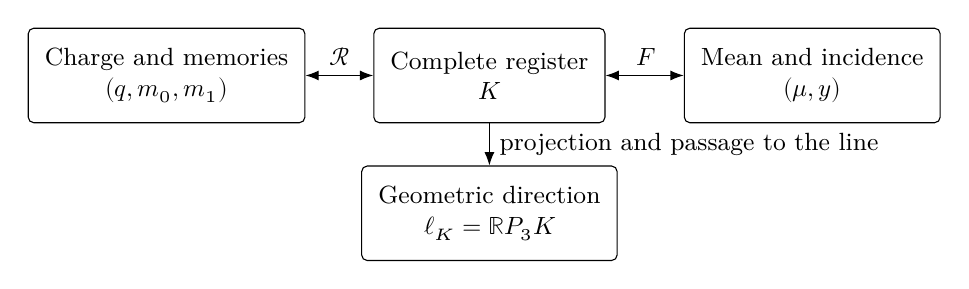
\begin{tikzpicture}[>=Latex, every node/.style={font=\small},
  box/.style={draw,rounded corners=2pt,align=center,
              inner sep=6pt,minimum height=12mm}]
 \node[box] (memory) at (0,0) {Charge and memories\\$(q,m_0,m_1)$};
 \node[box] (register) at (4.1,0) {Complete register\\$K$};
 \node[box] (incidence) at (8.2,0) {Mean and incidence\\$(\mu,y)$};
 \node[box] (direction) at (4.1,-1.75)
    {Geometric direction\\$\ell_K=\RR P_3K$};
 \draw[<->] (memory) -- node[above] {$\mathcal R$} (register);
 \draw[<->] (register) -- node[above] {$F$} (incidence);
 \draw[->] (register) -- node[right] {projection and passage to the line}
    (direction);
\end{tikzpicture}
\caption{The charge and the two compatible memories reconstruct the twelve
coordinates. The mean and the incidence component provide another
reversible representation of the same register. The geometric direction
is a subsequent reduction with positive-dimensional fibers.}
\label{rev4:ki:figure}
\end{figure}

This composition also determines the positive partition in
\ref{sec:memory}. If \(q>0\), its lengths are recovered through
\begin{equation}
 d_j=\frac1{12}+\frac{1}{6q}
             \bigl(P_0\mathcal I^{\mathsf T}y\bigr)_j,
 \qquad y=\frac16\mathcal I P_0K.
 \label{rev4:ki:positive-lengths}
\end{equation}
The twelve conditions \(d_j>0\) are the equations of the positive
chart expressed in incidence coordinates. With
\(t_j=\sum_{r\leq j}d_r\), the ordered minors
\(t_j-t_i=\sum_{i<r\leq j}d_r\) are reconstructed from
\((\mu,y)\) or from \((q,m_0,m_1)\). Thus the positivity of
the minors and the isometric preservation of incidence are related
by explicit maps. The former is an inequality in the ordered chart;
the latter is an identity of inner products.

\subsection{Recovery of polarization and scope of the reductions}
\label{rev4:ki:direction-subsection}

The realization of the twelve positions on the cosets of
\(A_5/C_5\) determines the three-dimensional projector
\[
 P_3=\frac3{60}\sum_{a\in A_5}
               \chi_3(a^{-1})\varrho(a).
\]
Here \(\varrho\) is the permutation representation and \(\chi_3\)
the three-dimensional character chosen in the marked chart. Its
representatives, character values, and effective matrix are fixed in
\eqref{eq:leech-projectors}; Lemma~\ref{lem:leech-u} proves
\(P_3=P_3^{\mathsf T}=P_3^2\),
\(\operatorname{rank}P_3=3\) and \(P_3\mathbf1=0\).
In this chart, the register direction is obtained through
\begin{equation}
 u_K=P_3P_0K=P_3Lm
     =\frac16P_3P_0\mathcal I^{\mathsf T}y.
 \label{rev4:ki:direction-reconstruction}
\end{equation}
The equalities follow from the two inverses already proved. The same
direction is therefore recovered from the memories or from the
incidence component; the mean is preserved to reconstruct \(K\),
even though the three-dimensional projector annihilates it.

For the register in \eqref{eq:leech-K}, the exact evaluation
\eqref{eq:leech-u-norm} gives
\[
 \|u_K\|^2=
       \frac{6638585+2275584\sqrt5}{20}>0.
\]
The line \(\ell_K=\RR u_K\) and the transverse complement
\(V_{10}(K)=V_0\cap u_K^\perp\) are thus determined.
Its projector is
\begin{equation}
 P_{10}(K)=P_0-
       \frac{u_Ku_K^{\mathsf T}}{\|u_K\|^2}.
 \label{rev4:ki:rank-ten}
\end{equation}
Indeed, the second summand is a rank-one orthogonal projector
contained in \(V_0\); its product with \(P_0\), in either order,
equals itself. Squaring \eqref{rev4:ki:rank-ten} recovers the same
operator, and its trace is \(11-1=10\). We obtain
\(V_0=\ell_K\oplus^\perp V_{10}(K)\).
This is the reduction that subsequently enters the polarization of
the twelve lattice planes.

Incidence also transports these operators. On \(E_{\rm inc}\), the
operator \(\widehat P_3=U_WP_3U_W^*\) satisfies
\(\widehat P_3U_W=U_WP_3\); the identity follows from
\(U_W^*U_W=I_{V_0}\). Transporting \(P_{10}(K)\) in the same
way preserves its rank and inner product. The correspondence between
the two representations is therefore established on vectors and
operators, as well as on their dimensions.

The need to preserve the different components admits precise checks.
The centered observation of \(k\) coincides with that of
\(k+c\mathbf1\) for every \(c\), whereas their charges differ
by \(12c\). In particular, \(k=0\) and \(k=\mathbf1\) have
the same centered incidence component and different means. The
coordinate \(\mu\) is exactly the information separating these two
registers. Likewise, \(u_{ak+b\mathbf1}=a u_k\) for \(a\ne0\);
the resulting line coincides with \(\ell_k\), even though the
amplitude and mean change. These identities describe the fibers of
the maps on the stated ambient space.

The extraction \(k\mapsto\{j:k_j\geq729\}\) has other fibers.
For the specific register \(K\), both \(K\) and \(K+e_1\)
have support \(\{4,6,9,10\}\), where \(e_1\) is the first
standard basis vector. These are two different ambient vectors with
the same tetrad. This check characterizes the information loss of the
support map; the terminal selection of the register remains fixed by
its prior construction. The flag \(B_K\subset H^-_\alpha\) also
preserves the hexad determined by the signs before the carry, whose
agreement with the incidence selection is proved in
Proposition~\ref{prop:lf-flag}.

The common result of these compositions is an explicit mathematical
continuity. Compatible memory reconstructs the register; its
uniform--centered decomposition determines an isometric incidence
representation; reconstruction of its lengths determines the positive
chart; and three-dimensional projection determines the deformation
direction. The tetrad and flag preserve the incidences used by the
exceptional constructions, whereas \(F\) preserves the entire
dodecaphasic register. The enriched history, in turn, retains the
orientation, path, and prolongation that place this register within
the joint discrete structure of the continuum.

% HMT provenance: output/EXTREMA_MEDIA_RAZON_NARRACION_Y_REVISION_20260916/
% ARTICULO/ES/source/libro/01_acoplamiento.tex, lib01:cadena-registro and lib01:K.
% Direction: ARTICULO/ES/source/sections/k_direccion_dimensional.tex.
% Status of the networks, charts, and flows in this appendix: FORMALIZACION_NUEVA.
% The extraction of K and the projector P_3 are RESULTADO_RECUPERADO.
\section{Planar boundary measurement, Plücker coordinates, and positive mutations}
\label{app:network-cluster}

The dodecaphasic representation of the enriched state admits a positive
realization whose network, coordinates, and chart changes can be written
out completely. The starting composition is
\[
 \mathrm{APP}\longrightarrow\mathrm{TRIT}\longrightarrow\mathrm{TPK}
 \longrightarrow x_{\rm term}\longrightarrow\mathcal R_{12}
 \longrightarrow(b^{90},b^{120},Q_{\rm TPK})
 \longrightarrow U_{\rm sgn}\longrightarrow K.
\]
This reading acts on the enriched state preserving the two sheets,
orientation, carry, memory, and boundary. The already generated register is
\[
 K=(234,543,140,729,659,824,621,58,914,794,146,601),
 \qquad Q=\sum_{r=1}^{12}K_r=6263.
\]
Its extraction is recovered exactly from the two channels and total charge:
\[
 b^{90}=(-495,-116,-684,108,601,-90,-173,-88,313,560,-397,461),
\]
\[
 b^{120}=(-425,-281,-481,671,-255,30,475,-543,680,251,6,-128).
\]
On the position orbits \((r,r+3,r+6,r+9)\), for \(r=1,2,3\),
let \(B_r=\sum_{j=0}^3b^{120}_{r+3j}\) and
\(d_{r,j}=b^{90}_{r+3j}\). We obtain
\[
 s_1=(Q+2B_1+B_2)/3,\quad s_2=s_1-B_1,\quad s_3=s_2-B_2,
\]
\[
 U^{(r)}=(s_r,d_{r,1}-d_{r,3},d_{r,0}+d_{r,2},d_{r,0}-d_{r,2}),
 \qquad K|_r=\tfrac14H_4U^{(r)},
\]
\[
 H_4=\begin{pmatrix}1&1&1&1\\1&1&-1&-1\\1&-1&1&-1\\1&-1&-1&1\end{pmatrix},
 \qquad H_4^2=4I_4.
\]
The network constructed below realizes the positive values produced by
this extraction. Its combinatorial form is a subsequent formalization
of the register, with stated origin and orientation.

\subsection{Directed acyclic network and determinants of nonintersecting paths}

For a positive register of length \(L\), set
\[
 d_r=K_r/Q>0,\qquad t_0=0,\qquad
 t_j=\sum_{r=1}^jd_r\quad(1\le j\le L).
\]
Thus \(t_L=1\). The \(L\) separations produce \(L+1\) marked
points; in the dodecaphasic case there are thirteen points.
The matrix realizing them is
\begin{equation}
 C(d)=\begin{pmatrix}1&1&\cdots&1\\t_0&t_1&\cdots&t_L\end{pmatrix}.
 \label{eq:nc-path-matrix}
\end{equation}
The Grassmannian \(\operatorname{Gr}(2,L+1)\) identifies rank-two
matrices under invertible changes of the two rows. Its positive part
consists of classes admitting all ordered minors of order two strictly
positive.

Construct a directed network with vertices \(a_j,b_j\), for
\(0\le j\le L\), and sinks \(q_j\). There are horizontal edges
\(a_{j-1}\to a_j\) and \(b_{j-1}\to b_j\), of weight one;
vertical edges \(a_j\to b_j\), of weight \(d_j\), for \(j\ge1\);
and edges \(b_j\to q_j\), of weight one. The ordered sources are
\(b_0,a_0\). The two rows are drawn horizontally, the vertical edges
descend, and the sinks exit below the lower row. This drawing is planar,
and the orientation is acyclic. The boundary measurement \(M_{ij}\)
is the sum of the products of weights of all paths from source \(i\)
to sink \(q_j\).
The path network has two sources and \(L+1\) sinks, hence \(L+3\)
external connections. The matrix it realizes has \(L+1\) columns.
The plabic seed introduced below has precisely \(L+1\) boundary
vertices and constitutes another presentation of its coordinates;
these two boundary counts are kept explicit.

\begin{theorem}[Boundary measurement and register minors]
\label{thm:nc-network}
The boundary measurement of this network is \(M=C(d)\).
For \(0\le i<j\le L\),
\begin{equation}
 \Delta_{ij}(C(d))=t_j-t_i=\sum_{r=i+1}^{j}d_r>0.
 \label{eq:nc-minor-gap}
\end{equation}
The same number is the sum of weights of the vertex-disjoint path
pairs \(b_0\to q_i\), \(a_0\to q_j\).
\end{theorem}
\begin{proof}
The lower source has a unique path to each sink, of weight one.
A path from \(a_0\) to \(q_j\) descends exactly once, along an
edge of index \(1\le r\le j\); its weight is \(d_r\). This
proves the matrix formula. The lower path to \(q_i\) occupies all
vertices \(b_0,\ldots,b_i\). A path from the other source to
\(q_j\) is therefore disjoint from it precisely when it descends
at \(i<r\le j\). Its sum of weights is the right-hand side of
\eqref{eq:nc-minor-gap}. The pair with exchanged destinations always
shares a vertex. Expanding the determinant cancels all intersecting
pairs and retains exactly the disjoint ones. Here the determinantal
mechanism of nonintersecting paths has been verified directly for the
specific network.
\end{proof}

Identification of planar-network measurements with cells of the
nonnegative Grassmannian provides their subsequent geometric recognition;
see A. Postnikov,
\href{https://arxiv.org/abs/math/0609764}{\emph{Total positivity,
Grassmannians, and networks}}. The preceding proof also gives a finite
formula for every minor without using a metrological value.

The collection \(d_r>0\), \(\sum_rd_r=1\), has dimension \(L-1\).
Its map to the Grassmannian is injective: if the rows of \(C(d)\)
and \(C(d')\) generate the same plane, the second rows differ by an
affine transformation; the conditions \(t_0=t'_0=0\) and
\(t_L=t'_L=1\) fix that transformation. In particular, for \(L=12\)
one obtains an eleven-dimensional collection inside the twenty-two-dimensional
positive cell. The point lies in the top cell; the collection retains its
own dimension. The thirteen points and twelve separations thus have
different mathematical roles.

Allowing \(d_r\ge0\) preserves nonnegativity. When \(d_r=0\),
consecutive columns \(r-1\) and \(r\) coincide and form parallel
elements of the matroid. The rank remains two because \(t_0=0\)
and \(t_L=1\). The bases are exactly the pairs \(i<j\) crossing
some positive separation. This degeneration produces strata of
consecutive incidence. A zero column, which would give a loop,
corresponds to a different operation from the coincidence of two
nonzero columns.

\subsection{Triangulation seed and exchange relation}

Let \(N=L+1\), and consider the vertices \(0,\ldots,L\) of a
convex polygon in cyclic order. To each side or diagonal \((i,j)\),
assign the coordinate \(A_{ij}=\Delta_{ij}(C(d))\), with ordered
indices. The fan triangulation from vertex zero has diagonals
\((0,j)\), \(2\le j\le L-1\). Its sides are frozen variables,
and its diagonals are mutable variables. The quiver is obtained by
cyclically orienting the three sides of each triangle and canceling
opposite arrow pairs. This is a seed of type \(A_{N-3}\); for the
dodecaphasic register, its type is \(A_{10}\).

The seed has an explicit plabic realization. Place a black vertex inside
each triangle; at the polygon vertices, place a white vertex if it is
incident to a diagonal, and a black one otherwise. Join the centers to
the three corners of their triangles, remove the original sides, and
contract edges between same-colored vertices. Add a boundary leaf at
each marked vertex. This construction follows the triangulation
algorithm of Kodama and Williams,
\href{https://people.math.harvard.edu/~williams/papers/KW-ArxivVersion.pdf}
{\emph{KP solitons and total positivity for the Grassmannian}, Algorithm 12.1}.
The coordinate labels of this seed are evaluated at the minors already
produced by the two-row network. For a mutable face, the
\(\mathcal X\)-type coordinate is the ratio of products of incident
\(\mathcal A\) coordinates prescribed by its quiver column; in a
quadrilateral it will be written explicitly as a cross-ratio.
Changing the graph changes the chart of these minors while preserving
their provenance.

\begin{theorem}[Positive exchange in the register realization]
\label{thm:nc-ptolemy}
For four vertices \(a<b<c<d\),
\begin{equation}
 A_{ac}A_{bd}=A_{ab}A_{cd}+A_{ad}A_{bc}.
 \label{eq:nc-ptolemy}
\end{equation}
Consequently, the diagonal change \((a,c)\leftrightarrow(b,d)\)
is evaluated through
\[
 A_{bd}=\frac{A_{ab}A_{cd}+A_{ad}A_{bc}}{A_{ac}}>0.
\]
All triangulations provide compatible positive charts on the same
realization \(C(d)\).
\end{theorem}
\begin{proof}
Substituting \(A_{ij}=t_j-t_i\) reduces the equality to
\[
 (t_c-t_a)(t_d-t_b)
 =(t_b-t_a)(t_d-t_c)+(t_d-t_a)(t_c-t_b).
\]
Expanding both sides proves the identity. The differences are positive;
therefore each flip preserves a positive evaluation, and the quotient
is defined. Connectivity of triangulations by flips allows passage
between them through these exchanges. The cluster interpretation of
the Plücker relation is the subsequent recognition developed by
J. Scott in
\href{https://arxiv.org/abs/math/0311148}{\emph{Grassmannians and Cluster
Algebras}}. The algebraic proof of the specific evaluation is already
contained in the displayed identity.
\end{proof}

\subsection{Refinement of separations and naturality of exchanges}

Let \(B\ge2\). At depth \(n\), each separation \(d_r\) is
divided into \(B^n\) equal consecutive separations:
\[
 d^{(n)}_{(r-1)B^n+c}=d_r/B^n,
 \qquad 1\le c\le B^n.
\]
This defines \(LB^n+1\) points and a matrix \(C_n\). If
\(\iota_n(j)=Bj\) identifies a point with its same-position
descendant, then
\begin{equation}
 C_{n+1}|_{\iota_n(\{0,\ldots,LB^n\})}=C_n,
 \qquad
 \Delta_{\iota_n(i),\iota_n(j)}(C_{n+1})=\Delta_{ij}(C_n).
 \label{eq:nc-refinement}
\end{equation}
The refined network replaces each vertical edge of weight \(d\)
by a sequence of \(B\) descent positions, with weights \(d/B\).
The path sum between inherited endpoints remains \(d\).
Composition of refinements preserves this equality because finite
sums are grouped associatively.

\begin{proposition}[Naturality on inherited endpoints]
\label{prop:nc-inherited}
Every exchange \eqref{eq:nc-ptolemy} among four inherited endpoints
commutes exactly with refinement. Every old triangulation extends to
one of the refined polygon while preserving its interior triangles:
the polygons added between consecutive endpoints are triangulated
outside those triangles. Flips between old diagonals then preserve
their exchange relations.
\end{proposition}
\begin{proof}
The first conclusion follows by substituting the equality in
\eqref{eq:nc-refinement} for each minor. For the second, preserve
the chords joining consecutive old endpoints and triangulate each
outer pocket formed by the new marks. These regions have disjoint
interiors. The two triangles incident to an old diagonal remain
unchanged, and so do their quadrilateral and Ptolemy identity.
\end{proof}

This naturality specifies the endpoints on which it acts. An old
side becomes a diagonal of the larger polygon when new vertices
are added along its boundary arc. A formerly frozen variable can
therefore be mutable in the enlarged problem. The preceding
compatibility is exact compatibility of the evaluation system and
inherited flips. An inclusion of seed patterns with the same
coefficient regime is obtained by keeping these chords and the new
auxiliary diagonals frozen. This states the operation that preserves
the seed; increasing depth and performing a mutation remain different
operations.

\subsection{Projective diagonal action and invariance of cross-ratios}

If \(\lambda_j>0\), the column action
\(C\mapsto C\operatorname{diag}(\lambda_0,\ldots,\lambda_L)\) gives
\[
 A_{ij}\longmapsto\lambda_i\lambda_j A_{ij}.
\]
It preserves positivity and all strata defined by vanishing minors.
The cross-ratio associated with a quadrilateral is
\begin{equation}
 X_{abcd}=\frac{A_{ab}A_{cd}}{A_{ad}A_{bc}}>0.
 \label{eq:nc-crossratio}
\end{equation}
The four factors \(\lambda_a\lambda_b\lambda_c\lambda_d\) cancel
exactly. Consequently, every positive diagonal column action fixes
\(X_{abcd}\), even if it depends on a parameter and has determinant
one. Changing column weights preserves the projective point of each
column; their cross-ratios express this preservation. For the register
to change the projective shape, it must act on the ordered separations.

\subsection{Register-directed positive deformation of separations}

The corpus fixes the representation of the twelve positions and its
orthogonal projector \(P_3\) onto the three-dimensional sector.
With \(P_{11}=I_{12}-J_{12}/12\), the recovered direction is
\[
 u=P_3P_{11}K=P_3K\in\mathbf1^\perp.
\]
In the stated chart, setting \(r=\sqrt5\), its exact evaluation is
\begin{align*}
u=(&-495/4-233r/10,\ 403/4+169r/10,\ -403/4-169r/10,\\
   &495/4+233r/10,\ 601/4+1031r/10,\ 203/4+211r/5,\\
   &-203/4-211r/5,\ -601/4-1031r/10,\ 313/4+569r/10,\\
   &162+219r/20,\ -162-219r/20,\ -313/4-569r/10).
\end{align*}
We retain \(\sum_ru_r=0\) and
\(\|u\|^2=(6638585+2275584\sqrt5)/20>0\).

For \(s\in\mathbb R\), define the deformation of the weights by
\begin{equation}
 d_r(s)=\frac{K_re^{su_r}}{\sum_{\ell=1}^{12}K_\ell e^{su_\ell}},
 \qquad t_j(s)=\sum_{r=1}^jd_r(s),\qquad C(s)=C(d(s)).
 \label{eq:nc-gap-flow}
\end{equation}
The formula uses the already generated register and its direction.
It is a new analytic realization of the reader; the parameter \(s\)
measures its deformation. When the internal output
\(\rho_A=\pi_{\rm HMT}/\varphi_{\rm HMT}^2\) is used, writing
\(s=\tau\log\rho_A\) expresses exactly the same collection.
This reparametrization acts after the generation of the constants.
Identifying \(s\) or \(\tau\) with a physical time requires the
temporal law of the corresponding reader.

\begin{theorem}[Shape change, positivity, and compatibility with depth]
\label{thm:nc-shape-flow}
The collection \eqref{eq:nc-gap-flow} belongs to
\(\operatorname{Gr}_{>0}(2,13)\) for every real \(s\) and preserves
\(t_0=0\), \(t_{12}=1\). For \(i<j\), let
\[
 \mu_{ij}(s)=
 \frac{\sum_{r=i+1}^jK_ru_re^{su_r}}{\sum_{r=i+1}^jK_re^{su_r}},
 \qquad
 \mu(s)=\frac{\sum_rK_ru_re^{su_r}}{\sum_rK_re^{su_r}}.
\]
Then
\begin{equation}
 \frac{d}{ds}\log A_{ij}(s)=\mu_{ij}(s)-\mu(s),
 \quad
 \frac{d}{ds}\log X_{abcd}(s)
 =\mu_{ab}(s)+\mu_{cd}(s)-\mu_{ad}(s)-\mu_{bc}(s).
 \label{eq:nc-crossratio-derivative}
\end{equation}
The deformation commutes with every refinement assigning the successors
of separation \(r\) the weight \(d_r/B\) and the same velocity \(u_r\).
\end{theorem}
\begin{proof}
All exponential factors and all \(K_r\) are positive. Normalization
makes the separations sum to one; the minors are sums of positive
separations by \eqref{eq:nc-minor-gap}. Differentiating the logarithm of
\[
 A_{ij}(s)=\frac{\sum_{r=i+1}^jK_re^{su_r}}
                      {\sum_rK_re^{su_r}}
\]
gives the first identity. The combination of four logarithms in
\eqref{eq:nc-crossratio} cancels the four global means with their
signs and gives the second. Finally, replacing \(K_r\) by \(B\)
copies of \(K_r/B\) with identical \(u_r\) preserves numerator
and denominator when the successors are grouped. The equality holds
for all parameters, at any depth, and for every composition of refinements.
\end{proof}

There is an exact witness that this collection changes shape. For the
first four endpoints,
\begin{equation}
 X_{0123}(0)=\frac{1560}{23711},\qquad
 \left.\frac{d}{ds}\log X_{0123}(s)\right|_{s=0}
 =-\frac{309899}{917}-\frac{268596}{4585}\sqrt5<0.
 \label{eq:nc-nontrivial-witness}
\end{equation}
The calculation uses only the first three separations
\((234,543,140)\) and their already recovered velocities. The strict
inequality proves an effective projective motion. The Ptolemy identities
remain exact during this motion, since they apply to the columns
\((1,t_j(s))\) at every parameter value. The register thus controls
a positive shape deformation and, simultaneously, a system of charts
that remains compatible with it.

The proved scope brings together a rank-two planar network, its explicit
measurement, a triangulation plabic seed, all its mutations by flips,
naturality of inherited endpoints, and a deformation of cross-ratios
directed by \(K\). Each operation has a verifiable domain and result.
Comparison of this realization with enriched temporal dynamics and
the material branch uses their respective reading maps; no coordinate
identity replaces those maps.

\section{Rank-one amplituhedral geometries and residue compatibility}
\label{sec:k-poligono-amplituhedral}

The dodecaphasic register allows positive data, Grassmannian domain,
kinematic image, covering, degree on cells, and canonical form to be
assembled explicitly. The first result concerns the two-dimensional
amplituhedron with parameters \((n,k,m)=(13,1,2)\); the construction
then extends to rank-one cyclic polytopes of higher dimension.
This is a subsequent geometric realization of the register produced
by APP--TRIT--TPK. The stated additional operation is lifting an ordered
rational partition by powers. This choice fixes a particular realization;
subsequent physical correspondences retain their own readers and conditions.

The provenance of the register preserves the composition
\[
 x_{\mathrm{term}}\longmapsto\mathcal R_{12}(x_{\mathrm{term}})
 \longmapsto(b^{90},b^{120},Q_{\mathrm{TPK}})
 \longmapsto U_{\mathrm{sgn}}\longmapsto K.
\]
APP preserves both sheets and their remainders and quotients; TRIT
orients the regime of each transition; TPK transports and updates
the state with carry, boundary, route, and memory. The representation
\(K\) is read in the same system of enriched states that jointly
generates the continuum. Its signed extraction and Hadamard inversion
produce
\begin{equation}
 K=(234,543,140,729,659,824,621,58,914,794,146,601),
 \qquad S_K=\sum_{j=1}^{12}K_j=6263.
 \label{eq:polygon-K}
\end{equation}
The geometric proof uses the positivity of these twelve coordinates,
their order, and their total. Its coefficients come from that extraction,
not from retrospective selection of a physical value.

\subsection{Rational partition and positive lift}

Define thirteen rational partition points:
\begin{equation}
 t_0=0,\qquad t_i=\frac{K_1+\cdots+K_i}{S_K}\quad(1\leq i\leq12),
 \qquad Z_i=(1,t_i,t_i^2)^\mathsf T,\qquad Z=(Z_0\ \cdots\ Z_{12}).
 \label{eq:polygon-Z}
\end{equation}
Their numerators, with common denominator \(6263\), are
\[
 (0,234,777,917,1646,2305,3129,3750,3808,4722,5516,5662,6263).
\]
Thus \(0=t_0<t_1<\cdots<t_{12}=1\). The labeled partition and
the total preserve the register through the exact inverse
\begin{equation}
 K_i=S_K(t_i-t_{i-1}).
 \label{eq:polygon-recover-K}
\end{equation}
The partition preserves the proportions; retaining \(S_K\) also
preserves the integer scale.

\begin{proposition}[Strictly positive kinematic data]
\label{prop:polygon-vandermonde}
The matrix \(Z\) has rank three, and all its ordered minors of size
three are positive. For \(0\leq a<b<c\leq12\),
\begin{equation}
 \langle abc\rangle:=\det(Z_a,Z_b,Z_c)
 =(t_b-t_a)(t_c-t_a)(t_c-t_b)>0.
 \label{eq:polygon-minors}
\end{equation}
\end{proposition}
\begin{proof}
Subtract the first column from the last two and expand along the
first row. Each difference \(t_j^2-t_a^2\) factors as
\((t_j-t_a)(t_j+t_a)\), giving the stated product. The strictly
increasing partial sums prove positivity. Any of these minors
establishes rank three.
\end{proof}

\subsection{Image, fibers, and degree-one cells}

The Grassmannian \(\operatorname{Gr}_{\geq0}(1,13)\) is the
projective space of nonnegative nonzero vectors
\(c=(c_0,\ldots,c_{12})\), modulo positive scaling.
The chart \(\sum c_j=1\) identifies it with the closed
twelve-dimensional simplex. Define
\begin{equation}
 \Phi_Z:\operatorname{Gr}_{\geq0}(1,13)\longrightarrow\mathbb P^2,
 \qquad[c]\longmapsto\left[\sum_{j=0}^{12}c_jZ_j\right].
 \label{eq:polygon-map}
\end{equation}
In the chart \(Y_0=1\), let \(v_j=(t_j,t_j^2)\) and
\(P_K=\operatorname{conv}(v_0,\ldots,v_{12})\).

\begin{theorem}[Polygonal amplituhedron of the register]
\label{thm:polygon-amplituhedron}
The closed image of \(\Phi_Z\) is exactly the convex polygon
\(P_K=\mathcal A_{13,1,2}(Z)\), of dimension two with thirteen
vertices. The image of the strictly positive Grassmannian is the
interior of \(P_K\). The eleven cells
\begin{equation}
 \mathcal S_i=\{[c]:c_0,c_i,c_{i+1}>0,\
 c_j=0\text{ if }j\notin\{0,i,i+1\}\},\qquad 1\leq i\leq11,
 \label{eq:polygon-cells}
\end{equation}
map bijectively, with degree one and positive orientation, onto the
interiors of \(T_i=[v_0,v_i,v_{i+1}]\). Their closures cover \(P_K\),
and their interiors are pairwise disjoint.
\end{theorem}
\begin{proof}
Under the normalization \(\sum c_j=1\), the map is
\(c\mapsto\sum c_jv_j\), whose image is the convex hull.
The minors in \eqref{eq:polygon-minors} show that every ordered
triple has positive orientation. Each consecutive side leaves all
other vertices strictly to its left; so does the final side from
\(v_{12}\) to \(v_0\). All points are therefore extreme vertices
of a convex polygon.

Every combination with \(c_j>0\) is interior, since for any
supporting line some vertex lies strictly in the interior half-plane.
Conversely, let \(y\) be interior and \(b=13^{-1}\sum v_j\).
For sufficiently small \(\varepsilon>0\),
\(y'=(y-\varepsilon b)/(1-\varepsilon)\) remains in the polygon.
Writing \(y'=\sum a_jv_j\), \(a_j\geq0\), \(\sum a_j=1\), gives
\(y=\sum((1-\varepsilon)a_j+\varepsilon/13)v_j\), with all
coefficients positive.

The diagonals from \(v_0\) divide the polygon into the eleven
triangles. On each triple support, the barycentric coordinates are
unique because \(\langle0,i,i+1\rangle>0\); their explicit inverse
appears in \eqref{eq:polygon-barycentric}. Each support defines a
rank-one positroid cell with coordinates \([1:a:b]\), \(a,b>0\),
at those positions. A directed planar network with one source and
three paths of weights \(1,a,b\) to the three destinations realizes
these coordinates by boundary measurement. The positive determinant
proves orientation and degree one.
\end{proof}

The generic fiber of the full map has dimension ten:
\(\sum c_j=1\), \(\sum c_jt_j=x\), and \(\sum c_jt_j^2=y\)
are three independent equations in thirteen coordinates.
For interior \(y\), the fiber contains a strictly positive point,
so its intersection with the simplex has dimension \(13-3=10\).
Degree one concerns the triangular cells; the two-dimensional form
is obtained through these cells.

\subsection{Canonical form and oriented residues}

For \(Y=(1,x,y)^\mathsf T\), define
\begin{equation}
 \ell_{ab}(Y)=\det(Z_a,Z_b,Y)
 =(t_b-t_a)\{y-(t_a+t_b)x+t_at_b\}.
 \label{eq:polygon-lines}
\end{equation}
The expression also holds when \(b<a\). For \(a<b<c\), let
\(D_{abc}=\langle abc\rangle\) and
\begin{equation}
 \lambda_a=\frac{\ell_{bc}}{D_{abc}},\qquad
 \lambda_b=\frac{\ell_{ca}}{D_{abc}},\qquad
 \lambda_c=\frac{\ell_{ab}}{D_{abc}},\qquad
 \lambda_a+\lambda_b+\lambda_c=1.
 \label{eq:polygon-barycentric}
\end{equation}
The affine orientation is \(dx\wedge dy\). Fix the boundary convention
\(\operatorname{Res}^{\partial}(\eta\wedge du/u)=\eta|_{u=0}\):
the normal differential occupies the last position. In dimension two,
the Poincaré residue placing \(du/u\) first has the opposite sign.
The following cancellations uniformly use the stated convention.

\begin{theorem}[Rational form and cancellation of diagonals]
\label{thm:polygon-form}
The canonical form of the oriented triangle \([v_a,v_b,v_c]\) is
\begin{equation}
 \Omega_{abc}=
 \frac{D_{abc}^2\,dx\wedge dy}
 {\ell_{ab}(Y)\ell_{bc}(Y)\ell_{ca}(Y)}.
 \label{eq:polygon-triangle-form}
\end{equation}
The canonical form of the polygon is
\begin{equation}
 \boxed{\displaystyle
 \Omega_{P_K}(x,y)=
 \sum_{i=1}^{11}
 \frac{t_it_{i+1}(t_{i+1}-t_i)\,dx\wedge dy}
 {(y-t_ix)\{y-(t_i+t_{i+1})x+t_it_{i+1}\}(t_{i+1}x-y)}.}
 \label{eq:polygon-full-form}
\end{equation}
The poles of interior diagonals cancel. The only polar divisors are
the thirteen lines of the exterior sides. Parametrizing each side
from its initial to its final vertex by \(s\in[0,1]\), its boundary
residue is \(ds/[s(1-s)]\).
\end{theorem}
\begin{proof}
The form of the barycentric simplex is
\(d\lambda_b\wedge d\lambda_c/(\lambda_a\lambda_b\lambda_c)\).
The Jacobian satisfies
\(dx\wedge dy=D_{abc}\,d\lambda_b\wedge d\lambda_c\).
Substituting \eqref{eq:polygon-barycentric} gives
\eqref{eq:polygon-triangle-form}. For \(a=0\), canceling the three
scalar factors of the lines gives each summand of
\eqref{eq:polygon-full-form}.

On side \(ab\), set \(\lambda_c=u\),
\(\lambda_b=(1-u)s\), \(\lambda_a=(1-u)(1-s)\). Then
\[
 \Omega_{abc}=\frac{ds}{s(1-s)}\wedge\frac{du}{u(1-u)}.
\]
The residue is the form of the oriented interval. Two adjacent
triangles induce opposite orientations on their diagonal and produce
opposite residues. Since all poles are simple, a vanishing residue
removes the diagonal pole as a divisor. Each exterior side appears
once. The homogeneous formula has degree zero as a projective form
and has no other polar divisors. If two rational projective forms
had the same residues and no other poles, their difference would be
a holomorphic two-form on \(\mathbb P^2\), necessarily zero.
This proves characterization and uniqueness.
\end{proof}

We use the conventional notion of positive geometry through logarithmic
poles and canonical boundary residues, developed by
N.~Arkani-Hamed, Y.~Bai, and T.~Lam, \emph{Positive Geometries and Canonical
Forms}, JHEP 11 (2017), 039,
\url{https://arxiv.org/abs/1703.04541}, Sections 2, 3, 5.2, 6.1, and 7.2.
The selection of the coefficients of the present polygon precedes this
recognition and comes from \(K\).

\subsection{Carry refinement on the fixed geometry}

In a positively oriented triangle \(T=[A,B,C]\), write
\begin{equation}
 Y(u,r)=(1-u)A+u\{(1-r)B+rC\},\qquad 0<u,r<1.
 \label{eq:polygon-blowdown}
\end{equation}
Vertex \(A\) corresponds to \(u=0\), and the opposite side to
\(u=1\). The form becomes
\begin{equation}
 \Omega_T=\frac{du}{u(1-u)}\wedge\frac{dr}{r(1-r)}.
 \label{eq:polygon-product-form}
\end{equation}
Let \(B_0\geq2\) be a stated integer base, distinct from vertex
\(B\). The coordinate \(r\) admits the remainder-and-carry update
\begin{equation}
 c=\lfloor B_0r\rfloor,\qquad r'=B_0r-c,\qquad
 r=\frac{c+r'}{B_0}.
 \label{eq:polygon-carry}
\end{equation}
The endpoints retain their boundary marks. The digit \(c\) remains
as memory and allows the update to be inverted. The charts of the
two affine transports should be specified. The subcell zoom acts
on \(r\in[c/B_0,(c+1)/B_0]\) through \(r'=B_0r-c\).
By contrast, transport of the lifted pair
\(L_c(x,y)=(B_0x-c,B_0y+c)\), with \(x+y=M\), changes the
total mass to \(B_0M\) and expresses the coordinate
\[
 \frac{B_0x-c}{B_0M}=\frac{x}{M}-\frac{c}{B_0M}.
\]
These maps have different domains and normalizations. Both preserve
the carry in the enriched state and admit recovery with their scale
data. The following proof uses the subcell zoom and the geometric
partition it identifies.

\begin{theorem}[Exact invariance under subdivision with memory]
\label{thm:polygon-carry}
Let \(s_j=j/B_0\) and \(W_j=(1-s_j)B+s_jC\).
The triangles \(T_j=[A,W_j,W_{j+1}]\), \(0\leq j<B_0\),
subdivide \(T\) and satisfy
\begin{equation}
 \sum_{j=0}^{B_0-1}\Omega_{T_j}=\Omega_T.
 \label{eq:polygon-carry-additivity}
\end{equation}
The equality remains valid at every finite depth and for any ordered
rational partition of the side. Subdividing the eleven triangles
of \(P_K\) leaves \(\Omega_{P_K}\) exactly invariant.
\end{theorem}
\begin{proof}
The regions \(r\in[s_j,s_{j+1}]\) cover \(T\) with disjoint
interiors. In the common coordinates,
\[
 \Omega_{T_j}=\frac{du}{u(1-u)}\wedge
 \frac{(s_{j+1}-s_j)\,dr}{(r-s_j)(s_{j+1}-r)}.
\]
The rational identity
\[
 \frac{s_{j+1}-s_j}{(r-s_j)(s_{j+1}-r)}
 =\frac1{r-s_j}+\frac1{s_{j+1}-r}
\]
telescopes: each interior term cancels the one from the adjacent
subinterval. This leaves \(1/r+1/(1-r)=1/[r(1-r)]\).
This proves equality of rational forms; iteration gives every finite
depth. The proof uses only \(s_0=0<s_1<\cdots<s_N=1\), so it
covers nonuniform partitions. The change
\(r'=(r-s_j)/(s_{j+1}-s_j)\) locally returns the unit form.
The carry word identifies the subcell, and its inverse recovers
the previous coordinate. The new interior poles cancel through the
same telescoping identity.
\end{proof}

The preceding sum assembles the complete geometric partition. When a
survival reader selects only some histories, its image is the union
of the selected subcells and its form is the corresponding sum;
it agrees with the form of the full polygon precisely when that union
covers it with oriented multiplicity one. The covering criterion for
a specific selection of histories is therefore expressed by a
checkable condition on its cell chain.

This refinement preserves the fixed polygon. Inserting a new point
\((t,t^2)\) on the parabola between consecutive parameters
\(a<t<b\) produces another geometry: the chord height minus
\(t^2\) is \((t-a)(b-t)>0\), and the new point lies outside
the previous polygon. The proved invariance concerns rectilinear
subdivision of cells, whose exterior boundary remains fixed.

\subsection{Triangulation changes and positive reparametrization}

For four ordered vertices \(A,B,C,D\), we have
\begin{equation}
 \Omega_{ABC}+\Omega_{ACD}=\Omega_{ABD}+\Omega_{BCD}.
 \label{eq:polygon-flip}
\end{equation}
Both sides have the same exterior residues and cancel their interior
diagonal; their equality follows from the proved uniqueness.
It is also checked by multiplying through by their linear denominators.
Every change between triangulations of a convex polygon decomposes
into these diagonal changes, so the form is independent of triangulation.
Identification with cluster coordinates must additionally preserve
the variety and its change relations.

If \(D=\operatorname{diag}(d_0,\ldots,d_{12})\), \(d_j>0\), then
\begin{equation}
 \mathcal A_{13,1,2}(ZD)=\mathcal A_{13,1,2}(Z).
 \label{eq:polygon-rescale}
\end{equation}
The automorphism \([c]\mapsto[Dc]\) reparametrizes the kinematic map.
In the affine chart, \(c_j\) changes to
\(c_jd_j/\sum_\ell c_\ell d_\ell\), which again ranges over the
simplex. The image and its canonical form remain unchanged.
Displacement of a parametrized history and change of the entire
geometric set are thus distinguishable operations.

\subsection{Rank-one extension to higher dimensions}

For \(2\leq m\leq12\), define
\begin{equation}
 Z_i^{(m)}=(1,t_i,t_i^2,\ldots,t_i^m)^\mathsf T,\qquad
 P_K^{(m)}=\operatorname{conv}
 \{(t_i,t_i^2,\ldots,t_i^m):0\leq i\leq12\}.
 \label{eq:polygon-higher-lift}
\end{equation}
The ordered maximal minors are the Vandermonde products
\(\prod_{a<b}(t_{i_b}-t_{i_a})>0\). The matrix has rank \(m+1\).
The image of \(\operatorname{Gr}_{\geq0}(1,13)\) is the cyclic
polytope \(P_K^{(m)}=\mathcal A_{13,1,m}(Z^{(m)})\), of dimension
\(m\); its generic fiber has dimension \(12-m\). Here we use the
mathematical extension of the amplituhedral definition to any \(m\);
customary applications to amplitudes impose their own values of \(m\).

The triangulation is determined by the fixed label order. Choose the
least vertex of a polytope, recursively triangulate all facets not
containing it, and take cones from that vertex. Induction begins with
points. A line from the initial vertex to an interior point meets
the opposite boundary in a facet; this proves covering. Uniqueness
of the intersection point and compatibility of the restrictions
induced by the same order prove that interiors are disjoint and
intersections are common faces. Dimension decreases at each step,
so the procedure terminates. This is a pulling triangulation
determined by the labels.

For an oriented simplex \(T=[p_0,\ldots,p_m]\) of this triangulation,
let
\[
 A_T=(p_1-p_0\ \cdots\ p_m-p_0),\qquad
 (\lambda_1,\ldots,\lambda_m)^\mathsf T=A_T^{-1}(x-p_0),
 \qquad\lambda_0=1-\sum_{j=1}^m\lambda_j.
\]
Orient its vertices so that \(\det A_T>0\).
Its canonical form is
\begin{equation}
 \Omega_T(x)=
 \frac{dx_1\wedge\cdots\wedge dx_m}
 {\det(A_T)\prod_{j=0}^m\lambda_j(x)},\qquad
 \Omega_{P_K^{(m)}}=\sum_{T}\Omega_T.
 \label{eq:polygon-higher-form}
\end{equation}
The barycentric change proves the formula and that the kinematic
restriction to the support of \(T\) has degree one. The residues
are the face forms with signs induced by orientation. On an interior
face, the two orientations are opposite and the total residue vanishes.
On an exterior face, the sum of the forms in that face's triangulation
remains. Induction on dimension proves that this sum is its canonical
form. Repeating the residue along a flag of faces reaches the vertices,
where the normalization is \(\pm1\). This gives residue correspondence
in every codimension for this rank-one collection.

The same proof covers any compatible simplicial subdivision of the
fixed polytope: interior faces cancel and exterior faces preserve the
residues. Nonexistence of top-degree holomorphic forms on
\(\mathbb P^m\) ensures uniqueness of the rational form.
In particular, refinement stability, covering, and residues are
settled in this collection of dimensions \(2,\ldots,12\).
Grassmannian degrees \(k>1\) retain their specific maps and
proof obligations.

\section{Moment matrices and higher-rank amplituhedral realizations}
\label{sec:higher-rank}
The partition of the dodecaphasic record extends the rank-one
construction to explicit higher-rank points. The same thirteen
ordered nodes simultaneously provide positive Plücker minors
and a positive-definite moment form. These two positivities are
obtained from a single list of intervals; the second proves that the
composition preserves the required rank.

Let \(d_j=K_j/Q\), where \(Q=\sum_{j=1}^{12}K_j=6263\), and define
\[
 t_0=0,\qquad t_j=\sum_{r=1}^jd_r.
\]
Positivity of the twelve blocks gives
\(0=t_0<t_1<\cdots<t_{12}=1\). For each \(2\le k\le9\), set
\[
 C^{(k)}_{ai}=t_i^a\quad(0\le a<k),\qquad
 Z^{(k)}_{bi}=t_i^b\quad(0\le b<k+4),\qquad 0\le i\le12.
\]
The convention \(t_i^0=1\) includes the zero node. Thus, \(C^{(k)}\)
is a \(k\times13\) matrix, while \(Z^{(k)}\) has
size \((k+4)\times13\).

\begin{theorem}[Positivity and rank of the moment realization]
The matrix \(C^{(k)}\) represents a point of
\(\Gr_{>0}(k,13)\), and all ordered maximal minors of
\(Z^{(k)}\) are positive. The matrix
\[
 Y^{(k)}=C^{(k)}(Z^{(k)})^{\mathsf T},\qquad
 Y^{(k)}_{ab}=\sum_{i=0}^{12}t_i^{a+b},
\]
has rank \(k\). In particular, for the positive external datum
\(Z^{(k)}\) already constructed from the record,
\[
 [Y^{(k)}]\in\mathcal A_{13,k,4}(Z^{(k)}),\qquad 2\le k\le9,
\]
where
\[
 \mathcal A_{13,k,4}(Z^{(k)})
 =\{[C(Z^{(k)})^{\mathsf T}]:[C]\in\Gr_{\ge0}(k,13)\}.
\]
\end{theorem}
\begin{proof}
A maximal minor of either initial matrix has the form
\[
 \det(t_{i_j}^{a})_{a=0}^{r-1}
 =\prod_{p<q}(t_{i_q}-t_{i_p})>0,
\]
for increasing indices. The inequality proves both Plücker
assertions. The initial \(k\times k\) block of \(Y^{(k)}\) is the
Hankel matrix \(H^{(k)}\). For \(x\ne0\),
\[
 x^{\mathsf T}H^{(k)}x
 =\sum_{i=0}^{12}\left(\sum_{a=0}^{k-1}x_at_i^a\right)^2>0.
\]
Indeed, a nonzero polynomial of degree less than \(k\le9\) cannot
vanish at thirteen distinct points. Hence \(H^{(k)}\) is positive definite,
its determinant is strictly positive and \(Y^{(k)}\) has rank
\(k\). Amplituhedral membership is then the composition of the
two preceding positive matrices, with rank already verified.
\end{proof}

In rank two, the proof takes the particularly explicit form
\[
 \det H^{(2)}=13\sum_i t_i^2-\left(\sum_i t_i\right)^2
 =\sum_{i<j}(t_j-t_i)^2>0.
\]
Node separation, produced by positivity of the record,
is thus converted into coercivity of a quadratic form. Each
fixed record corresponds to a specified point for each rank. The
complete coverage, triangulations and residues proved in the
preceding section retain their rank-one domain; the present theorem
adds the explicit collection of rank-two to rank-nine points and their moment
matrices. This distinction allows each proof to be reused within its
precise scope.

% Additive section. Does not modify the 211-page edition.
% Provenance and checks: internal documents in this same directory.
\section{Nonadic refinement, positive flags, and compatibility of moments}
\label{sec:dim-cofinal}

The length of a finite representation determines how many minors can be
formed from its columns. Refinement preserves inherited columns and
adds others with known provenance. Thus the dimension of a matrix
realization can grow without replacing the register that fixes its
separations. The following construction combines this growth with two
precise notions of compatibility: restriction of evaluations to the
previous marks and averaging of observables over descendant cells.
The former preserves polynomial flags; the latter preserves a
measure and separates the information increment into orthogonal details.

The starting datum is the dodecaphasic output already produced by
APP--TRIT--TPK. The two APP sheets preserve their complete divisions;
TRIT orients the regime, and the operator
\(U_t=\operatorname{Upd}_t\circ\operatorname{Tra}_t\circ
\operatorname{Sel}_t\) transports the enriched state. The prolongation
\(w_6\to w_{12}\to w_{18}\to w_{24}\to w_{30}\to R_{36}\to G_9\)
preserves phase return and memory advance. The joint discrete structure
of the continuum correlatively preserves the representations of that state,
with their sheets, orientation, memory, and boundaries. The regional
representations and the signed register come from this same state;
inversion of the latter gives
\[
 K=(234,543,140,729,659,824,621,58,914,794,146,601),
 \qquad Q=\sum_{j=1}^{12}K_j=6263.
\]
This output is used with its marks and orientation; the moment matrices
are subsequent realizations. The refinement index introduced below
counts subdivisions of the geometric reader. Identifying it with a
physical duration or a number of TPK microtransitions requires preserving
the clock of that other realization.

\subsection{Marked partitions and cofinal growth}

Write \(d_j=K_j/Q\), \(a_0=0\), and
\(a_j=\sum_{h=1}^j d_h\). For \(r\geq0\), define
\[
 L_r=12\,9^r,\qquad N_r=L_r+1,\qquad
 t_{r,(j-1)9^r+c}=a_{j-1}+\frac{c}{9^r}d_j,
 \quad 0\leq c\leq9^r.
\]
Shared endpoints are counted only once. The \(L_r\) cells are indexed
by \((j,c)\), with \(1\leq j\leq12\) and \(0\leq c<9^r\),
and have length \(\ell_{r,j,c}=d_j/9^r\). The expression of \(c\)
in \(r\) nonadic digits, including leading zeros, is also preserved.
A successor has index \(9c+h\), with \(0\leq h\leq8\); Euclidean
division recovers its predecessor and last digit. Shared endpoints retain
their boundary mark; the half-open interval convention only organizes
the cells and removes no mark.

\begin{proposition}[Cofinality and recovery of the register]
\label{prop:dim-grid}
The marks satisfy
\[
 0=t_{r,0}<t_{r,1}<\cdots<t_{r,L_r}=1,
 \qquad t_{r+1,9i}=t_{r,i}.
\]
The maximum length is \(h_r=(\max_jK_j)/(Q9^r)\), which tends
to zero. For every pair of integers \(k\geq1\), \(m\geq1\),
there is an \(r_0\) such that \(k+m\leq N_r\) for \(r\geq r_0\).
The register is recovered at any level through
\[
 K_j=Q\sum_{c=0}^{9^r-1}\ell_{r,j,c}.
\]
\end{proposition}
\begin{proof}
Each consecutive difference is \(d_j/9^r>0\). Replacing \(c\)
by \(9c\) in the next-level formula gives exactly the previous mark.
The nine successor lengths sum to the predecessor length; iteration proves
recovery. Finally, \(N_r=12\,9^r+1\) grows without bound.
An explicit choice is any \(r_0\geq0\) with
\(9^{r_0}\geq(k+m-1)/12\). The entire argument preserves \(Q\),
the block index, and the descent digits.
\end{proof}

Normalization determines the ratios \(K_j/Q\). Recovery of the
integers also uses the charge \(Q\) preserved by the register.
This distinguishes the normalized geometry from the scale information
accompanying its representation.

\subsection{Evaluation flags and realizations in every finite dimension}

For \(1\leq q\leq N_r\), let
\[
 V_r^{(q)}=(t_{r,i}^{\,a})_{0\leq a<q,\,0\leq i<N_r},
 \qquad F_r^q=\operatorname{row}V_r^{(q)}.
\]
The zeroth power is one at the zero node as well.

\begin{theorem}[Positive flag and arbitrary-rank composition]
\label{thm:dim-all-ranks}
The spaces \(F_r^q\) form a flag
\(F_r^1\subset F_r^2\subset\cdots\subset F_r^{N_r}\), with
\(\dim F_r^q=q\), and every matrix \(V_r^{(q)}\) has all its
ordered maximal minors strictly positive. For
\(k\geq1\), \(m\geq1\), \(k+m\leq N_r\), the matrices
\[
 C_r=V_r^{(k)},\quad Z_r=V_r^{(k+m)},\quad
 Y_r=C_rZ_r^{\mathsf T}
\]
satisfy
\[
 (Y_r)_{ab}=\sum_{i=0}^{L_r}t_{r,i}^{a+b},\qquad
 \operatorname{rank}Y_r=k,\qquad
 [Y_r]\in\mathcal A_{N_r,k,m}(Z_r).
\]
The construction reaches every finite pair \((k,m)\) through a
sufficiently deep level of the same marked partition.
\end{theorem}
\begin{proof}
For \(i_1<\cdots<i_q\), the corresponding minor is
\[
 \det(t_{r,i_b}^{a-1})_{a,b=1}^{q}
   =\prod_{a<b}(t_{r,i_b}-t_{r,i_a})>0.
\]
This proves rank, positivity, and the flag inclusions. The initial
\(k\times k\) block of \(Y_r\) is the Gram matrix of the evaluations
of \(1,t,\ldots,t^{k-1}\). For \(x\neq0\),
\[
 x^{\mathsf T}(Y_r)_{[0,k-1],[0,k-1]}x
 =\sum_i\left(\sum_{a=0}^{k-1}x_at_{r,i}^{a}\right)^2>0,
\]
because a nonzero polynomial of degree less than \(k\) cannot vanish
at the \(N_r\geq k+m\) distinct nodes. The block is invertible,
and \(Y_r\), which has \(k\) rows, has rank \(k\).
The stated membership is the application of the positive external
matrix \(Z_r\) to the positive point represented by \(C_r\).
\end{proof}

We use the mathematical convention
\[
 \mathcal A_{N,k,m}(Z)=
 \{[CZ^{\mathsf T}]:[C]\in\operatorname{Gr}_{\geq0}(k,N)\}.
\]
The definition for general \(m\) can be found in S.~N.~Karp,
L.~K.~Williams, and Y.~X.~Zhang,
\href{https://people.math.harvard.edu/~williams/papers/amplituhedron-plus.pdf}
{\emph{Decompositions of amplituhedra}}, Definition~1.1.
Here the external datum already comes from the partition expressed by HMT.
The conclusion constructs a determined collection of points and flags;
the dimensions of the ambient Grassmannian and of an atlas of its
image are objects additional to the ranks proved.

Let \(E_r:\mathbb R^{N_{r+1}}\to\mathbb R^{N_r}\) be restriction
to the positions \(9i\). For every \(q\leq N_r\),
\[
 E_r\bigl((V_{r+1}^{(q)})^{\mathsf T}x\bigr)
       =(V_r^{(q)})^{\mathsf T}x.
\]
Thus \(E_r:F_{r+1}^q\to F_r^q\) is an isomorphism on these
evaluation spaces: its two realizations identify the same polynomial
of degree less than \(q\). Composing restrictions agrees with direct
restriction. Minors on inherited indices preserve their value exactly.

\begin{proposition}[Recovery from a calibrated flag]
If the column order, endpoint marks, and calibration
\(t_{r,0}=0\), \(t_{r,L_r}=1\) are preserved, the plane \(F_r^2\)
determines the nodes and separations. Together with \(Q\) and the
descent marks, it determines \(K\).
\end{proposition}
\begin{proof}
The plane contains the constant vector and the node vector. Any other
coordinate that, together with the constant vector, generates the same
plane is \(a+bt\), with \(b\neq0\). The two calibrations fix
\(a=0\), \(b=1\). Consecutive differences recover the lengths,
and Proposition~\ref{prop:dim-grid} recovers the register.
\end{proof}

\subsection{Rank-one convex bodies and growth of the domain}

For \(m\geq1\) and \(m+1\leq N_r\), define
\[
 P_r^{(m)}=\operatorname{conv}
 \{(t_{r,i},t_{r,i}^2,\ldots,t_{r,i}^m):0\leq i\leq L_r\}.
\]
Normalizing a positive row of \(C\) as barycentric coefficients proves
\(\mathcal A_{N_r,1,m}(Z_r)=P_r^{(m)}\). The Vandermonde
determinant provides \(m+1\) affinely independent points, so the
body has dimension \(m\).

\begin{proposition}[Simplicial covering in finite dimension and convex limit]
\label{prop:dim-polytopes}
Every \(P_r^{(m)}\) admits a triangulation using its vertices, with
degree one over the interior of every simplicial cell. The sum of
their canonical forms has canceled interior residues. Moreover,
\[
 P_r^{(m)}\subseteq P_{r+1}^{(m)},\qquad
 \overline{\bigcup_{r\geq r_0}P_r^{(m)}}=
 \operatorname{conv}\{(t,t^2,\ldots,t^m):0\leq t\leq1\}.
\]
\end{proposition}
\begin{proof}
Order the vertices by their marks. In each face, choose its least
vertex; recursively triangulate the facets not containing it and form
the corresponding cones. Induction on dimension proves covering and
disjoint interiors, and the same rule on shared faces guarantees
compatibility. In each oriented simplex \([v_0,\ldots,v_m]\), with
matrix \(A=(v_1-v_0,\ldots,v_m-v_0)\) of positive determinant and
barycentric coordinates \(\lambda_0,\ldots,\lambda_m\), the
barycentric map is affine and invertible. Its form is
\[
 \Omega_{[v_0,\ldots,v_m]}=
 \frac{dx_1\wedge\cdots\wedge dx_m}
 {\det A\prod_{j=0}^{m}\lambda_j}.
\]
The residual restriction to each face is its oriented form. Two
adjacent simplices induce opposite orientations on their common face,
so the interior residues cancel. This is the same triangulation and
residue operation applied in the previous rank-one realization, with
the number of vertices now increased by refinement.

Inclusion of inherited nodes proves inclusion of the bodies. The mesh
tends to zero, so the sampled curves are dense in the compact moment
curve. Every finite convex combination of curve points is approximated
by combinations using nodes from a common level. Conversely, all the
bodies lie in the compact convex hull of the curve. Both inclusions
prove the equality.
\end{proof}

Cancellation of residues acts on a triangulation or subdivision of a
fixed body. Passing from \(P_r^{(m)}\) to \(P_{r+1}^{(m)}\)
adds vertices and can enlarge the body. Their forms belong to their
respective domains. The preceding convex limit specifies convergence
of the bodies without imposing an identity between their forms.

\subsection{Calendar measure and convergence of nodal moments}

Let \(F_K:[0,1]\to[0,1]\) be the increasing piecewise affine
function taking \((j-1)/12\) to \(a_{j-1}\) and \(j/12\) to
\(a_j\). On the corresponding interval, its slope is \(12d_j>0\).
The transported calendar measure is
\[
 \mu_K=(F_K)_*(ds),\qquad
 \frac{d\mu_K}{dt}=\frac1{12d_j}\quad
 (a_{j-1}<t<a_j).
\]
Each initial interval has mass \(1/12\), and each level-\(r\)
cell has mass \(1/L_r\). This choice assigns equal weight to the
calendar positions before realizing their lengths. The length measure
\(dt\) is another reader; the two coincide when all initial
separations are equal.

Its moments are rational and determined by \(K\):
\begin{equation}
 M_p=\int_0^1t^p\,d\mu_K(t)
   =\frac1{12(p+1)}\sum_{j=1}^{12}
       \frac{a_j^{p+1}-a_{j-1}^{p+1}}{d_j},\qquad p\geq0.
 \label{eq:dim-moments}
\end{equation}
\begin{proposition}[Recovery through moments and quantiles]
\label{prop:dim-moment-recovery}
The full sequence \((M_p)_{p\geq0}\) determines \(\mu_K\).
If \(H_K(t)=\mu_K([0,t])\) is its distribution function, then
\[
 a_j=H_K^{-1}(j/12),\qquad
 K_j=Q\bigl(H_K^{-1}(j/12)-H_K^{-1}((j-1)/12)\bigr).
\]
Consequently, the complete moments, the charge \(Q\), and the calendar
order recover the initial register.
\end{proposition}
\begin{proof}
Two probability measures on \([0,1]\) with the same moments have the
same integrals for all polynomials. Uniform approximation of continuous
functions by polynomials and finite mass extend this equality to all
continuous functions, which determine the Borel measure. The density
of \(\mu_K\) is positive and constant on each initial interval.
Its distribution is therefore continuous and strictly increasing, and
satisfies \(H_K(a_j)=j/12\). Inverting this equality and taking the
difference of endpoints prove the formulas.
\end{proof}

The nodal probability measure corresponding to Theorem
\ref{thm:dim-all-ranks} is
\(\nu_r=N_r^{-1}\sum_{i=0}^{L_r}\delta_{t_{r,i}}\).

\begin{theorem}[Limit of the nodal representation]
\label{thm:dim-nodal-limit}
We have \(\nu_r\rightharpoonup\mu_K\). If \(f\) is continuous,
\[
 \left|\int f\,d\nu_r-\int f\,d\mu_K\right|
 \leq \omega_f(h_r)+\frac{\operatorname{osc}(f)}{N_r},
\]
where \(\omega_f\) is its modulus of continuity. For \(p\geq1\),
the error of the moment of order \(p\) is bounded by
\(p h_r+1/N_r\). For every fixed pair \((k,m)\),
\[
 \frac1{N_r}Y_r\longrightarrow (M_{a+b})_{
     0\leq a<k,\,0\leq b<k+m}=:Y_\infty^{(k,m)},
 \qquad\operatorname{rank}Y_\infty^{(k,m)}=k.
\]
\end{theorem}
\begin{proof}
The measure assigning mass \(1/L_r\) to each left cell endpoint
approximates its integral with error at most \(\omega_f(h_r)\).
Indeed, each cell has that mass and diameter no greater than \(h_r\).
The measure \(\nu_r\) is \(L_r/N_r\) times this measure plus
\(\delta_1/N_r\), adding at most
\(\operatorname{osc}(f)/N_r\). For \(f(t)=t^p\), the Lipschitz
constant is \(p\). Convergence of each entry follows from these
bounds. The initial block of the limit matrix is positive definite:
the integral of the square of a nonzero polynomial is positive,
because \(\mu_K\) has strictly positive density on every open
interval of \([0,1]\). Thus the limit preserves rank \(k\).
\end{proof}

Nodal moments change exactly through the addition of nodes.
If \(\mathcal J_r\) is the set of new positions and
\(z_q(t)=(1,t,\ldots,t^{q-1})^{\mathsf T}\), then
\[
 V_{r+1}^{(q)}(V_{r+1}^{(q)})^{\mathsf T}
 =V_r^{(q)}(V_r^{(q)})^{\mathsf T}
  +\sum_{i\in\mathcal J_r}z_q(t_{r+1,i})z_q(t_{r+1,i})^{\mathsf T}.
\]
Each summand is positive semidefinite. The same update holds for the
rectangular matrices \(Y_r\), using \(z_kz_{k+m}^{\mathsf T}\).
The equality expresses the change in counting measure; normalization
and the preceding theorem describe its limit. The rank-\(k\) limit
object has coordinates in a finite Grassmannian, whereas the external
data \(Z_r\) belong to the different representations at each level.

\subsection{Cell averages, compatible operators, and orthogonal detail}

For a cell \(I_{r,i}=[b_{r,i},b_{r,i}+\ell_{r,i}]\), set
\[
 a_{r,i}^{(p)}=
 \frac{(b_{r,i}+\ell_{r,i})^{p+1}-b_{r,i}^{p+1}}
 {(p+1)\ell_{r,i}},\qquad
 A_r^{(q)}=(a_{r,i}^{(p)})_{0\leq i<L_r,\,0\leq p<q}.
\]
These are the monomial means with respect to the conditional probability
of \(\mu_K\) on each cell. This probability is uniform on the cell,
although \(\mu_K\) is not the global length measure.

Let \(\mathcal H_r=\mathbb R^{L_r}\) with inner product
\(\langle x,y\rangle_r=L_r^{-1}\sum_i x_i y_i\). The map
\(J_r:\mathcal H_r\to\mathcal H_{r+1}\) repeats a predecessor's value
on its nine successors. Its adjoint \(R_r=J_r^*\) averages those
nine values. We have \(R_rJ_r=I\).

\begin{theorem}[Exact compatibility and moment balance]
\label{thm:dim-cell-balance}
For every \(p\geq0\),
\[
 R_r a_{r+1}^{(p)}=a_r^{(p)},\qquad
 \frac1{L_r}\sum_i a_{r,i}^{(p)}=M_p.
\]
Define
\[
 D_r^{(q)}=A_{r+1}^{(q)}-J_rA_r^{(q)},\quad
 G_r^{(q)}=\frac1{L_r}(A_r^{(q)})^{\mathsf T}A_r^{(q)}.
\]
Then
\[
 R_rD_r^{(q)}=0,\qquad
 G_{r+1}^{(q)}=G_r^{(q)}+
       \frac1{L_{r+1}}(D_r^{(q)})^{\mathsf T}D_r^{(q)},
\]
and
\[
 G_r^{(q)}\longrightarrow H_K^{(q)}=(M_{a+b})_{0\leq a,b<q}.
\]
The details and initial level reconstruct all levels. For
\(q\leq L_r\), the matrix \(A_r^{(q)}\) has rank \(q\), and
all ordered minors of order \(q\) are positive.
\end{theorem}
\begin{proof}
The nine successors have equal masses, and their intervals partition the
predecessor interval. Additivity of the integral gives the first identity;
summing over all cells gives the second. The decomposition
\(A_{r+1}=J_rA_r+D_r\) is orthogonal in each column because
\(R_rD_r=0\). Expanding its Gram matrix cancels the cross terms,
and \(J_r\) is an isometry. This proves the matrix balance.

The cellwise constant observable taking the value \(a_{r,i}^{(p)}\)
uniformly approximates \(t^p\), with error no greater than \(p h_r\)
for \(p\geq1\). It therefore converges in \(L^2(\mu_K)\), and
the inner products converge to \(M_{a+b}\). Reconstruction is
obtained by iterating \(A_{r+1}=J_rA_r+D_r\).

To prove the minors, choose \(q\) ordered cells. By multilinearity
and Fubini, the determinant of their averages is the mean over the
product of these cells of \(\prod_{a<b}(x_b-x_a)\). This integrand
is positive in the interior of the product because the cells are
disjoint and ordered. Their boundaries have measure zero. The mean
is strictly positive.
\end{proof}

The identity extends to the degree pair \(k\) and \(k+m\):
\[
 \overline Y_r=\frac1{L_r}(A_r^{(k)})^{\mathsf T}A_r^{(k+m)},
 \qquad
 \overline Y_{r+1}-\overline Y_r
 =\frac1{L_{r+1}}(D_r^{(k)})^{\mathsf T}D_r^{(k+m)}.
\]
For \(k+m\leq L_r\), the averaging matrices define a second
positive amplituhedral realization, with \(L_r\) columns, and
\(\overline Y_r\) has rank \(k\). These are cell averages,
whereas \(Y_r\) uses evaluations at \(N_r=L_r+1\) nodes. Both
realizations converge to \(Y_\infty^{(k,m)}\); their agreement
in the limit follows from the preceding proofs.

The operator version is equally explicit. For a continuous function
\(f\), let \(\Psi_r(f)\) be the diagonal operator of its conditional
means on \(\mathcal H_r\). It is linear, positive, and unital, and
\[
 R_r\Psi_{r+1}(f)J_r=\Psi_r(f).
\]
This equality is proved by applying both sides to each basis vector.
For \(X(t)=t\), the first two operators determine, cell by cell,
\[
 \Psi_r(X)_i=b_{r,i}+\frac{\ell_{r,i}}2,\qquad
 \Psi_r(X^2)_i-\Psi_r(X)_i^2=\frac{\ell_{r,i}^2}{12}.
\]
If \(v_{r,i}\) denotes this variance, the formula
\(\ell_{r,i}=\sqrt{12v_{r,i}}\) recovers the length; the first
identity recovers the initial endpoint. With orientation, marks, and
\(Q\), one again recovers \(K\). Averaging is a positive compression:
the displayed variance quantifies why \(\Psi_r(X^2)\) and
\(\Psi_r(X)^2\) are different operations.

\subsection{Transport of the measure and scope of dimensional growth}

Two positive lists of separations \(d\) and \(d'\), with the same
marks, determine an increasing piecewise affine homeomorphism
\(F=F_{K'}\circ F_K^{-1}\). It takes each cell to its corresponding
cell and satisfies \(F_*\mu_K=\mu_{K'}\). Hence
\[
 \mathcal U_F:L^2(\mu_K)\longrightarrow L^2(\mu_{K'}),
 \qquad\mathcal U_F f=f\circ F^{-1}
\]
is a surjective isometry. If \(P_r\) and \(P'_r\) are the
projections onto cellwise constant functions, then
\(P'_r\mathcal U_F=\mathcal U_FP_r\): conditional means are
transported because the masses of corresponding cells agree.
This applies in particular to the positive separation flow directed
by \(K\), preserving each block's direction in its successors. The
moments of the spatial coordinate may change; the isometry transports
the observable together with the measure and its projections.

The growth proved is cofinal in every finite external dimension.
It preserves a system of positive flags, an explicit collection of
amplituhedral points, complete convex bodies in rank one, and a measure
whose averaging operators are exactly compatible. Memory of the details
allows inversion of compression between levels. The rank-one covering
and residue proofs preserve their domain; for higher ranks, the present
result fixes matrices, positivity, recovery, compatibility, and limit
with explicit types. This separation locates the scope of each
construction within the same development without confusing dimension
growth, parametrization of a point, and classification of all cells
of an image.

\section{Genealogical moments, Jacobi operators, and spectral residues}
\label{sec:jacobi-generated}

The calendar-induced measure provides a link between cell geometry and
a positive spectral realization. This link uses the entire marked
partition: each of its twelve intervals preserves the same chronological
mass, whereas its length comes from the corresponding register
coordinate. The density exactly compensates for that length.
Consequently, the spatial distribution of the measure retains the
anisotropy of the register even though the distribution among windows
is uniform.

Let \(K_j>0\), \(Q=\sum_{j=1}^{12}K_j\), \(d_j=K_j/Q\), and
\(t_j=\sum_{i\leq j}d_i\), with \(t_0=0\). The probability measure
used in this section is
\[
 \dd\mu_K(t)=\sum_{j=1}^{12}
 \frac{\mathbf1_{[t_{j-1},t_j]}(t)}{12d_j}\,\dd t.
\]
Shared endpoints have measure zero. Its moments are rational for
every integer register:
\begin{equation}
 m_r=\int_0^1t^r\,\dd\mu_K(t)
 =\frac1{12(r+1)}\sum_{j=1}^{12}
   \frac{t_j^{r+1}-t_{j-1}^{r+1}}{d_j},\qquad r\geq0.
 \label{eq:jacobi-moments}
\end{equation}
The equality \(m_0=1\) expresses conservation of total mass. For
each \(n\geq1\), the Hankel matrix \(H_n=(m_{a+b})_{0\leq a,b<n}\)
is positive definite: its quadratic form is the integral of the square
of a nonzero polynomial over an interval where the density is positive.
This observation allows passage from moments to an operator without
choosing a target spectrum.

\begin{theorem}[Tridiagonal recurrence determined by the partition]
\label{thm:jacobi-recurrence}
There is a unique sequence of monic polynomials \(p_n\), of degree
\(n\), orthogonal for \(\mu_K\). If
\[
 h_n=\int p_n^2\,\dd\mu_K>0,\qquad
 a_n=\frac{\int t p_n^2\,\dd\mu_K}{h_n},\qquad
 \beta_n=\frac{h_n}{h_{n-1}}>0\quad(n\geq1),
\]
then \(p_0=1\), \(p_1=t-a_0\), and
\begin{equation}
 p_{n+1}(t)=(t-a_n)p_n(t)-\beta_np_{n-1}(t),\qquad n\geq1.
 \label{eq:jacobi-recurrence}
\end{equation}
All coefficients \(a_n,\beta_n\) are rational for the stated integer
register. In the orthonormal basis \(\psi_n=p_n/\sqrt{h_n}\),
the compression of multiplication by \(t\) to polynomials of degree
less than \(n\) has the symmetric matrix
\[
 J_n=\begin{pmatrix}
 a_0&\sqrt{\beta_1}&&0\\
 \sqrt{\beta_1}&a_1&\ddots&\\
 &\ddots&\ddots&\sqrt{\beta_{n-1}}\\
 0&&\sqrt{\beta_{n-1}}&a_{n-1}
 \end{pmatrix}.
\]
\end{theorem}
\begin{proof}
Positivity of \(H_n\) guarantees that the linear system imposing
orthogonality on a monic polynomial has a unique solution. Since its
coefficients are rational moments, the solution is rational. Expand
\(tp_n\) in the monic basis through degree \(n+1\). For
\(j\leq n-2\), symmetry of the inner product gives
\(\langle tp_n,p_j\rangle=\langle p_n,tp_j\rangle=0\).
Only the terms of degrees \(n+1,n,n-1\) remain. Their coefficients
are, respectively, \(1,a_n,h_n/h_{n-1}\), proving the recurrence.
Normalization by \(\sqrt{h_n}\) turns the two adjacent coefficients
into \(\sqrt{\beta_n}\).
\end{proof}

For the register expressed in Section~\ref{sec:register}, the first
diagonal entry and the square of the first coupling are
\[
 a_0=m_1=\frac{71195}{150312},\qquad
 \beta_1=m_2-m_1^2=\frac{2206226167}{22593697344}.
\]
The first equality calculates the center of mass of the chronological
partition; the second calculates its dispersion and determines the
first link of the tridiagonal matrix. Both numbers are obtained by
integrating the generated lengths, and their structural meaning
precedes any decimal evaluation.

\begin{theorem}[Simple spectrum, quadrature, and positive residues]
\label{thm:jacobi-residues}
The eigenvalues \(\lambda_1<\cdots<\lambda_n\) of \(J_n\) are
simple and belong to \((0,1)\). There are unique weights \(w_i>0\),
summing to one, such that
\begin{equation}
 \int f(t)\,\dd\mu_K(t)=\sum_{i=1}^{n}w_i f(\lambda_i)
 \qquad(\deg f\leq2n-1).
 \label{eq:jacobi-quadrature}
\end{equation}
The resolvent observed at the unit constant \(e_0\) satisfies
\begin{equation}
 g_n(z)=\langle e_0,(zI-J_n)^{-1}e_0\rangle
       =\sum_{i=1}^{n}\frac{w_i}{z-\lambda_i}
       =\cfrac1{z-a_0-\cfrac{\beta_1}{z-a_1-
          \cfrac{\beta_2}{\ddots-\cfrac{\beta_{n-1}}{z-a_{n-1}}}}}.
 \label{eq:jacobi-resolvent}
\end{equation}
In particular, its poles and residues are obtained from the register
through the operations of taking moments, orthogonalization, and
compression.
\end{theorem}
\begin{proof}
For any nonzero polynomial \(p\) of degree less than \(n\),
\[
 0<\int_0^1 t|p(t)|^2\,\dd\mu_K(t)
   <\int_0^1 |p(t)|^2\,\dd\mu_K(t).
\]

The variational characterization places the spectrum of \(J_n\) in
\((0,1)\). Each subdiagonal entry is positive. The eigenvector
equations recursively determine all its coordinates from the first;
if that coordinate vanished, the entire vector would vanish. Every
eigenspace therefore has dimension one. Symmetry of the matrix gives
orthogonal diagonalization and simplicity of the spectrum. For unit
eigenvectors \(v_i\), set \(w_i=|\langle e_0,v_i\rangle|^2>0\).
Completeness of the eigenbasis gives \(\sum_iw_i=1\) and the first
expression for the resolvent.

By expansion of the determinant, the tridiagonal recurrence shows that
\(\det(tI-J_n)=p_n(t)\). For \(\deg f\leq2n-1\), Euclidean
division writes \(f=qp_n+r\), with \(\deg q,\deg r<n\).
Orthogonality makes the integral of \(qp_n\) vanish, and its
evaluation at the \(\lambda_i\) also vanishes. For \(r\) of degree
less than \(n\), successive multiplications of the constant by \(t\)
remain within the polynomial space up to the required degree; hence
\(\int r\,\dd\mu_K=\langle e_0,r(J_n)e_0\rangle\).
The spectral resolution proves the quadrature formula. Its uniqueness
follows from invertibility of the Vandermonde matrix evaluated at the
distinct roots. Finally, the Schur complement of the first row and
column of \(zI-J_n\), iterated over the trailing submatrices,
produces the continued fraction.
\end{proof}

\begin{figure}[htbp]
\centering
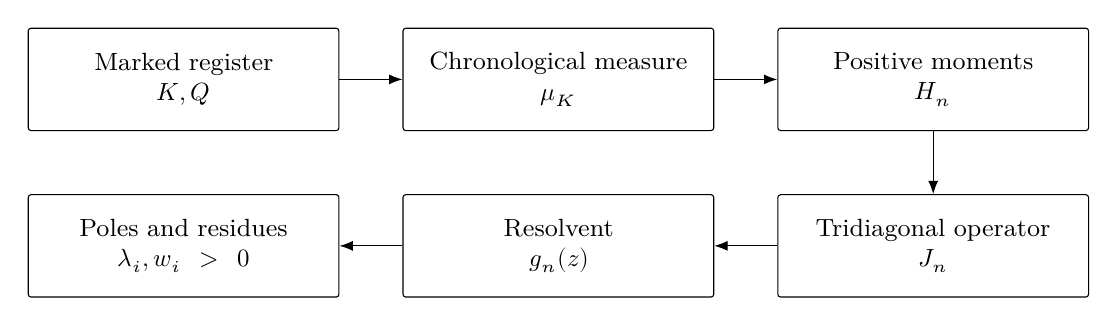
\begin{tikzpicture}[>=Latex, node distance=8mm and 8mm,
 every node/.style={font=\small}, box/.style={draw,rounded corners=1pt,
 text width=37mm,minimum height=13mm,align=center}]
\node[box] (k) {Marked register\\\(K,Q\)};
\node[box,right=of k] (m) {Chronological measure\\\(\mu_K\)};
\node[box,right=of m] (h) {Positive moments\\\(H_n\)};
\node[box,below=of h] (j) {Tridiagonal operator\\\(J_n\)};
\node[box,left=of j] (g) {Resolvent\\\(g_n(z)\)};
\node[box,left=of g] (w) {Poles and residues\\\(\lambda_i,w_i>0\)};
\draw[->] (k)--(m);\draw[->] (m)--(h);\draw[->] (h)--(j);
\draw[->] (j)--(g);\draw[->] (g)--(w);
\end{tikzpicture}
\caption{Spectral realization of the HMT partition. Cell geometry
determines the measure; positivity of its moments produces the operator
and the positive residues of its resolvent.}
\label{fig:jacobi-generated}
\end{figure}

The resolvent formula provides a spectral reading of spatial memory.
The positive weights describe how much the constant coordinate observes
of each mode; the poles are the algebraic frequencies of the compressed
multiplication operator. Moments of increasing order recover successive
details of the measure, and the continued-fraction coefficients preserve
this information through a local three-term recurrence. The classical
appearance of a Jacobi matrix is recognized after its coefficients have
been constructed from the HMT cells. The causal chain is fixed by
\[
 K\longmapsto(d,t)\longmapsto\mu_K\longmapsto(m_r)_{r\geq0}
 \longmapsto\bigl((a_n)_{n\geq0},(\beta_n)_{n\geq1}\bigr)
 \longmapsto(J_n,g_n).
\]

\begin{proposition}[Dimension and refinement compatibility]
\label{prop:jacobi-refinement}
The matrices \(J_n\) are compatible principal compressions of the
same bounded multiplication by \(t\) on \(L^2(\mu_K)\). Their
spectral measures \(\sum_iw_i\delta_{\lambda_i}\) converge weakly
to \(\mu_K\). If each nonadic subinterval is represented by its
midpoint and its mass \(1/(12\cdot9^r)\), the resulting atomic
measure \(\mu_{K,r}\) approximates the moments of \(\mu_K\).
For a fixed degree \(n\), construction from these moments recovers
the coefficients \(a_j,\beta_j\) of the same matrix as refinement
tends to infinite depth.
\end{proposition}
\begin{proof}
Orthogonalization of the complete sequence uses the same formulas as
\(n\) increases, so each principal block remains fixed. Quadrature
exactly reproduces any polynomial once \(2n-1\) exceeds its degree.
Uniform approximation of continuous functions on \([0,1]\) by
polynomials, together with total mass one, proves weak convergence.
The midpoint sums converge on each of the twelve intervals with its
constant density, and thus approximate all moments. In fixed dimension,
the orthogonalization coefficients are rational functions of finitely
many moments, with denominators formed from positive Gram determinants.
Convergence of these moments and positivity of the limit ensure
convergence of the coefficients.
\end{proof}

\begin{falsifier}
A zero length invalidates the stated density and can destroy the rank
of the moments. Replacing the fixed measure by unnormalized counts on
different meshes changes the operator. The residues of \(g_n\) are
spectral weights of the resolvent, whereas the residues of a canonical
form are defined on geometric divisors: identifying these notions
requires specifying the form and the corresponding map. Likewise,
\(J_n\) is dimensionless; identifying it with a physical Hamiltonian
requires the representation and the action and clock scale used by
that sector.
\end{falsifier}

\begin{theorem}[Faithfulness of the marked spectral realization]
\label{thm:jacobi-marked-faithfulness}
The infinite Jacobi operator \(J\), together with its unit cyclic
vector \(e_0\) and charge \(Q\), determines the register \(K\).
Two realizations of this type are unitarily equivalent through a map
preserving the marked vector and charge if and only if their registers
agree. The spectrum as a set, by contrast, is \([0,1]\) for every
positive register in the domain.
\end{theorem}
\begin{proof}
Polynomials are dense in \(L^2(\mu_K)\): first approximate continuous
functions and then use their density for the finite measure.
The constructed orthonormal basis defines a unitary map taking
\(e_n\) to \(\psi_n\). Under this map, \(J\) is multiplication
by \(t\), a bounded self-adjoint operator, and \(e_0\) represents
the constant function one. Therefore,
\[
 \langle e_0,J^re_0\rangle=m_r\qquad(r\geq0).
\]
These moments determine the measure: two measures with the same
moments agree on polynomials, then on continuous functions by uniform
approximation, and finally as Borel measures. Its distribution
\(F(t)=\mu_K([0,t])\) is continuous and strictly increasing.
Each initial interval has mass \(1/12\), so
\[
 t_j=F^{-1}(j/12),\qquad
 K_j=Q\bigl(F^{-1}(j/12)-F^{-1}((j-1)/12)\bigr).
\]
A unitary equivalence preserving \(e_0\) preserves the moments and
therefore the register. The converse follows from the unique
construction.

For the last statement, the density of \(\mu_K\) is positive on
every subinterval. Each \(\lambda\in[0,1]\) admits unit-norm
functions concentrated on progressively smaller intervals around
\(\lambda\), on which the norm of \((J-\lambda I)f\) tends
to zero. Thus the entire interval belongs to the spectrum. Outside
it, multiplication by \(1/(t-\lambda)\) is bounded and defines
the resolvent. This proves equality of the spectrum.
\end{proof}

The theorem distinguishes the extent of the spectrum from the
information it preserves relative to a marked observation. The same
spectral interval admits the different distributions of the collection;
the measure observed from the unit recovers the original separations.
The link with the Grassmannian representation is now reversible:
marked minors reconstruct \(K\), the register constructs
\((J,e_0,Q)\), and its moments and quantiles recover the same
register. Every reader factoring through \((K,\xi)\) therefore
has a marked spectral expression once the remaining coordinates
\(\xi\) are preserved. The spectral realization contains structure,
in addition to pole positions or eigenvalues.

\begin{figure}[htbp]
\centering
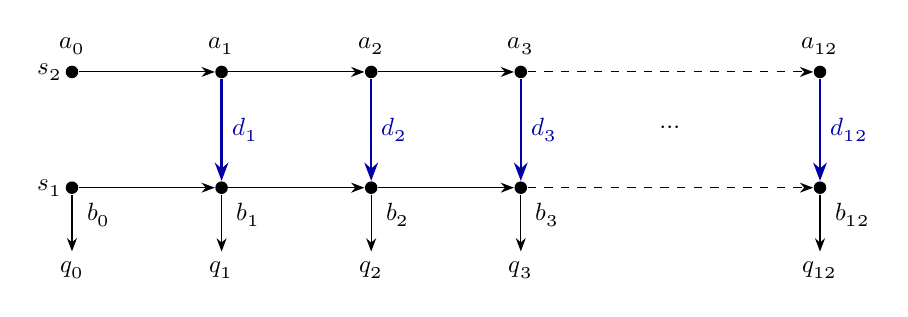
\begin{tikzpicture}[x=1.9cm,y=1.05cm,>=Stealth,font=\small]
\foreach \j/\lab in {0/0,1/1,2/2,3/3,5/12}{
  \node[circle,fill=black,inner sep=1.6pt,label=above:{$a_{\lab}$}] (a\j) at (\j,1.4) {};
  \node[circle,fill=black,inner sep=1.6pt,label=below right:{$b_{\lab}$}] (b\j) at (\j,0) {};
  \node (q\j) at (\j,-1) {$q_{\lab}$};
  \draw[->] (b\j) -- (q\j);
}
\foreach \j/\prev in {1/0,2/1,3/2}{
 \draw[->] (a\prev)--(a\j);\draw[->] (b\prev)--(b\j);
 \draw[->,blue!65!black,thick] (a\j)--node[right]{$d_{\j}$}(b\j);
}
\draw[->,blue!65!black,thick] (a5)--node[right]{$d_{12}$}(b5);
\draw[dashed,->] (a3)--(a5);\draw[dashed,->] (b3)--(b5);
\node at (4,.7) {$\cdots$};
\node[left] at (a0) {$s_2$};\node[left] at (b0) {$s_1$};
\end{tikzpicture}
\caption{Two-row planar network. Horizontal and outgoing edges
have weight one. Each path from the upper source descends exactly
once. For two destinations \(i<j\), disjoint pairs descend after
\(i\) and before \(j\); their total weight is
\(\Delta_{ij}=d_{i+1}+\cdots+d_j\). Dashed lines retain
the eight intermediate positions omitted only from the drawing.}
\end{figure}

\begin{figure}[htbp]
\centering
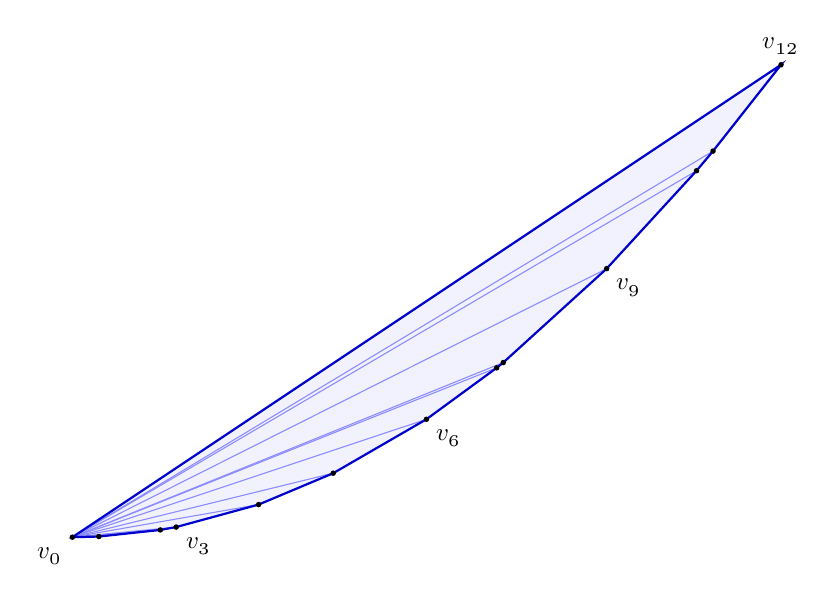
\begin{tikzpicture}[x=9cm,y=6cm,font=\small]
\foreach \j/\num in {0/0,1/234,2/777,3/917,4/1646,5/2305,6/3129,7/3750,8/3808,9/4722,10/5516,11/5662,12/6263}{
 \pgfmathsetmacro{\tx}{\num/6263}
 \coordinate (v\j) at (\tx,\tx*\tx);
}
\fill[blue!5] (v0)--(v1)--(v2)--(v3)--(v4)--(v5)--(v6)--(v7)--(v8)--(v9)--(v10)--(v11)--(v12)--cycle;
\foreach \j in {2,...,11}{\draw[blue!45,thin] (v0)--(v\j);}
\draw[blue!80!black,thick] (v0)--(v1)--(v2)--(v3)--(v4)--(v5)--(v6)--(v7)--(v8)--(v9)--(v10)--(v11)--(v12)--cycle;
\foreach \j in {0,...,12}{\fill (v\j) circle[radius=.035cm];}
\node[below left] at (v0) {$v_0$};
\node[below right] at (v3) {$v_3$};
\node[below right] at (v6) {$v_6$};
\node[below right] at (v9) {$v_9$};
\node[above] at (v12) {$v_{12}$};
\end{tikzpicture}
\caption{Rational polygon determined by the thirteen parameters
\(t_j\) in \eqref{eq:polygon-Z}, plotted with its actual coordinates
\((t_j,t_j^2)\). The triangulation from \(v_0\) has eleven cells.
Each interior diagonal receives two opposite residues. Five vertices
are labelled for legibility; all thirteen are represented.}
\end{figure}

\section{Weight flow, information geometry and Legendre duality}
\label{sec:convex-refinement}

Interval deformation admits an exact variational
description. Let \(d_j=K_j/Q>0\), \(\sum_jd_j=1\), and let \(u_j\) be the
coordinates of the direction \eqref{eq:u-main}. For \(s\in\RR\),
define
\begin{equation}
 Z(s)=\sum_{j=1}^{12}d_j e^{su_j},\qquad
 \psi(s)=\log Z(s),\qquad
 d_j(s)=\frac{d_j e^{su_j}}{Z(s)}.
 \label{eq:convex-partition}
\end{equation}
All exponential arguments are dimensionless. The parameter
\(s\) is the coordinate of this geometric deformation. Assigning
a physical duration belongs to a declared temporal reader.

\begin{theorem}[Strict convexity and dual coordinate]
The function \(\psi\) is analytic and strictly convex on \(\RR\).
If \(u_- =\min_j u_j\) and \(u_+=\max_j u_j\), the map
\(v=\psi'(s)\) is a diffeomorphism from \(\RR\) onto \((u_-,u_+)\).
For each \(v\) in that interval there is a unique coordinate \(s(v)\), and
\[
 \psi^*(v)=s(v)v-\psi(s(v)),\qquad
 (\psi^*)'(v)=s(v),\qquad
 (\psi^*)''(v)=\frac1{\psi''(s(v))}>0.
\]
\end{theorem}
\begin{proof}
The finite sums allow termwise differentiation. This gives
\begin{align}
 \psi'(s)&=\sum_jd_j(s)u_j=:\overline u(s),\notag\\
 \psi''(s)&=\sum_jd_j(s)(u_j-\overline u(s))^2.
 \label{eq:variance}
\end{align}
The weights are strictly positive and the \(u_j\) are not all equal;
the variance is therefore strictly positive. As \(s\) tends to
\(+\infty\), dividing numerator and denominator of \(\psi'\) by
\(e^{su_+}\) shows that only indices with \(u_j=u_+\) survive.
Thus \(\psi'(s)\to u_+\). The argument with \(u_-\) gives the opposite
limit. Monotonicity and the inverse function theorem provide
smooth bijectivity. The function \(sv-\psi(s)\) has its unique maximum
at \(s(v)\); differentiating the maximum value proves the two dual
identities.
\end{proof}

The evolution of each interval is
\begin{equation}
 \dot d_j(s)=d_j(s)\bigl(u_j-\overline u(s)\bigr).
 \label{eq:replicator}
\end{equation}
The derivatives sum to zero. Total length therefore remains
one while the internal lengths are redistributed. This conservation
of global scale allows the change in cross-ratios to be attributed to a
deformation of positions rather than a common dilation.

On the open simplex of weights, the metric
\(g_d(\xi,\zeta)=\sum_j\xi_j\zeta_j/d_j\), on tangent vectors
of sum zero, is positive. The linear function
\(F(d)=\sum_jd_ju_j\) has, with respect to this metric, exactly the
field in \eqref{eq:replicator} as its gradient, since
\[
 g_d\bigl(d_j(u_j-\overline u),\xi\bigr)
 =\sum_j(u_j-\overline u)\xi_j=\sum_ju_j\xi_j=dF(\xi).
\]
Consequently \(dF/ds=\psi''(s)>0\) along the flow. The
ascending character corresponds to this specific function and metric.

\begin{theorem}[Variational invariance under inherited subdivision]
For each interval \(j\), let \(r_{j,c}>0\),
\(\sum_c r_{j,c}=1\), be the relative weights of a fixed subdivision.
Assign to the subintervals
\[
 d_{j,c}=r_{j,c}d_j,\qquad u_{j,c}=u_j.
\]
The partition function, its logarithm, all its derivatives and the Legendre
transform agree exactly with those of the predecessor partition.
Furthermore, the flow commutes with summation over subintervals:
\[
 \sum_c d_{j,c}(s)=d_j(s),\qquad
 d_{j,c}(s)=r_{j,c}d_j(s).
\]
\end{theorem}
\begin{proof}
Grouping the finite sum gives
\[
 Z_{\rm ref}(s)=\sum_{j,c}r_{j,c}d_j e^{su_j}
 =\sum_j d_j e^{su_j}=Z(s).
\]
All conclusions follow from this identity and from dividing each
weight by the same \(Z(s)\). The same argument holds after any
finite number of subdivisions. For a countable subdivision, the sum of
positive terms converges to the same value when grouped by predecessor intervals.
\end{proof}

The inherited-direction hypothesis has verifiable content. If an
interval with direction \(a\) is divided into two halves with directions
\(a+b\) and \(a-b\), its contribution changes from
\(d e^{sa}\) to \(d e^{sa}\cosh(sb)\). For \(b\ne0\), equality
of partition functions fails even though the total weight at \(s=0\) is
the same. Geometric and variational conservation thus requires preserving
the relevant directional information as well. The proved identity
applies to inherited subdivision; its transport to a TPK update
that changes those directions is determined by composing the reader of that
update.

There is a regular Hamiltonian formulation of the dual coordinate. In the
cotangent plane with coordinates \((q,p)\), take
\(H(q,p)=\psi(p)\). The equations are
\(\dot q=\psi'(p)\), \(\dot p=0\). For velocities
\(\dot q\in(u_-,u_+)\), the Legendre transform gives
\[
 L(q,\dot q)=\psi^*(\dot q),\qquad
 \frac{\partial^2L}{\partial\dot q^2}>0.
\]
This system variationally realizes the potential of the interval flow.
Its equation \(\dot p=0\) shows that Hamiltonian time differs
from the parameter \(s\) traversing the collection \eqref{eq:convex-partition}.
Evaluation of \(H\) and \(L\) is preserved under the subdivision of the
theorem, because \(\psi\) and \(\psi^*\) remain identical.

In turn, any flow \(\dot d=F(d)\) admits, in a local chart
of the simplex, a cotangent lift with
\(\mathscr H(d,p)=p\cdot F(d)\). This second construction reproduces
the flow \eqref{eq:replicator} itself on its base, but its Hessian with respect
to \(p\) is zero. The two realizations answer different questions:
one produces a regular convex duality and the other transports dynamics
on a given base. This distinction preserves the meaning of Hamiltonian and
Lagrangian when comparing this geometry with the physical readers of the corpus.

% Bounded development: interval energy reader of the register K.
% Status: added formalization on K and the Schur identities
% already present in the corpus. No historical novelty is attributed to Schur.
\section{Dirichlet forms and variational equivalence of refinement}
\label{sec:energia-refinamiento-k}

The positive representation of the dodecaphasic register defines an
ordered partition through
\[
 K=(234,543,140,729,659,824,621,58,914,794,146,601),
 \qquad d_j=K_j/6263,
 \qquad t_i=\sum_{j=1}^id_j.
\]
The register is received from the composition
\(x_{\rm term}\mapsto\mathcal R_{12}\mapsto
(b^{90},b^{120},Q_{\rm TPK})\mapsto U_{\rm sgn}\mapsto K\),
subsequent to APP--TRIT--TPK and its enriched state, in accordance
with the readers reconstructed in \cite{hmtX}. This section applies
a quadratic reader to the resulting partition. Depths will be compared
through restrictions to inherited endpoints, so that every energy
coefficient retains its origin in an already produced positive separation.

The corpus contains a weighted difference energy for the graph of
the two memories and a Schur reduction of the complete forms.
Here these operations are brought together on the interval network
of the register. The specialization to conductances \(1/d_j\),
the interpolation operator, and its compatibility with deformation
of the separations constitute the formalization developed in this section.

\subsection{Reconstruction of separations from the stiffness matrix}

Let \(d=(d_1,\ldots,d_m)\), with \(d_j>0\), and let
\(f=(f_0,\ldots,f_m)\in\mathbb C^{m+1}\) be the values of an
observable at the partition endpoints. Define
\begin{equation}
 \mathcal E_d(f)=\sum_{j=1}^{m}\frac{|f_j-f_{j-1}|^2}{d_j},
 \qquad L_d=D^*\operatorname{diag}(d_1^{-1},\ldots,d_m^{-1})D,
 \label{eq:energia-intervalar}
\end{equation}
where \(D:\mathbb C^{m+1}\to\mathbb C^m\) is the oriented incidence
operator, \((Df)_j=f_j-f_{j-1}\), and the asterisk denotes the
Hermitian adjoint. Thus \(\mathcal E_d(f)=f^*L_df\).
The stiffness matrix has entries
\[
 (L_d)_{00}=d_1^{-1},\quad (L_d)_{mm}=d_m^{-1},\quad
 (L_d)_{ii}=d_i^{-1}+d_{i+1}^{-1}\quad(1\le i<m),
\]
\[
 (L_d)_{i-1,i}=(L_d)_{i,i-1}=-d_i^{-1},
\]
and all other entries vanish. It is Hermitian positive semidefinite,
its kernel consists of the constant functions, and its form is positive
definite on the quotient by that kernel. The complete matrix recovers
the separations through
\begin{equation}
 d_j=-\frac1{(L_d)_{j-1,j}}.
 \label{eq:recuperacion-d-rigidez}
\end{equation}

\begin{proposition}[Equivalence between separations and the complete nodal reader]
\label{prop:energia-bidireccional}
The map \(d\mapsto L_d\) is a bijection between
\((0,\infty)^m\) and the set of real symmetric tridiagonal matrices
whose entries immediately adjacent to the diagonal are negative and
whose row sums are zero. Its inverse is
\eqref{eq:recuperacion-d-rigidez}. The normalization
\(\sum_jd_j=1\) is equivalent to
\(\sum_{j=1}^m-1/(L_d)_{j-1,j}=1\).
\end{proposition}
\begin{proof}
The explicit formulas for \(L_d\) satisfy all the conditions.
Conversely, the negative adjacent entries determine unique positive
separations through \eqref{eq:recuperacion-d-rigidez}. The zero
sum of each row determines its diagonal entries as the sum of
incident conductances. Tridiagonality makes all remaining entries
zero. The matrix in \eqref{eq:energia-intervalar} is recovered
exactly; its positive semidefiniteness then follows from the
factorization \(D^*\operatorname{diag}(1/d_j)D\).
\end{proof}

The weighted discrete derivative \(J_j=(f_j-f_{j-1})/d_j\) is the
oriented flow of edge \(j\). At interior vertices,
\((L_df)_i=J_i-J_{i+1}\); at the endpoints,
\((L_df)_0=-J_1\) and \((L_df)_m=J_m\). The interior equation
\(L_df=0\) expresses that the flow has the same value on every edge.
This defines a quadratic observable of the interval reader;
its realization as a physical quantity requires the relevant dimensional chart.

\subsection{Harmonic interpolation, Schur complement, and detail reconstruction}

Refine each separation as
\(d_j=\sum_{c=1}^{r_j}\delta_{j,c}\), with \(\delta_{j,c}>0\).
Let \(\widetilde d\) be the concatenation of these separations,
\(R\) restriction to the old endpoints, and \(H\) the interpolation
defined by
\begin{equation}
 (Hf)_{j,c}=(1-\theta_{j,c})f_{j-1}+\theta_{j,c}f_j,
 \qquad
 \theta_{j,c}=\frac{\sum_{a=1}^c\delta_{j,a}}{d_j}.
 \label{eq:interpolacion-armonica-k}
\end{equation}
Shared endpoints are counted only once. We have \(RH=I\).

\begin{theorem}[Isometric refinement of the energy]
\label{thm:energia-schur-refinamiento}
For every vector of old values \(f\),
\begin{equation}
 H^*L_{\widetilde d}H=L_d,
 \qquad L_{\widetilde d}H=R^*L_d,
 \qquad
 \min_{Rg=f}\mathcal E_{\widetilde d}(g)=\mathcal E_d(f).
 \label{eq:isometria-energia-k}
\end{equation}
The minimizer is unique and equals \(Hf\). Every \(g\) admits
the unique decomposition
\begin{equation}
 g=H(Rg)+z,\qquad Rz=0,
 \qquad
 \mathcal E_{\widetilde d}(g)
 =\mathcal E_d(Rg)+\mathcal E_{\widetilde d}(z).
 \label{eq:detalle-energia-k}
\end{equation}
\end{theorem}
\begin{proof}
On an old edge, write \(h_c=g_{j,c}-g_{j,c-1}\), so that
\(\sum_ch_c=f_j-f_{j-1}=a\). If
\(h_c=\delta_{j,c}a/d_j+r_c\), then \(\sum_cr_c=0\) and
\[
 \sum_c\frac{|h_c|^2}{\delta_{j,c}}
 =\frac{|a|^2}{d_j}+\sum_c\frac{|r_c|^2}{\delta_{j,c}}.
\]
The equality follows by expansion; the cross term is proportional to
\(\sum_cr_c\) and vanishes. The minimum is attained exactly when
all \(r_c\) vanish, the condition determining
\eqref{eq:interpolacion-armonica-k}. Summing over the edges gives
the minimum and the energy decomposition. The flow of \(Hf\) is
constant within every old edge, so its interior components of
\(L_{\widetilde d}Hf\) vanish and its inherited components agree
with \(L_df\). This proves the second matrix identity; multiplying
by \(H^*\), using \(RH=I\), gives the first.
\end{proof}

The term \(\mathcal E_{\widetilde d}(z)\) is nonnegative and
vanishes exactly for \(z=0\): a zero-energy detail would be constant
and, vanishing at the inherited endpoints, would vanish throughout
the network. The pair \((Rg,z)\) preserves the complete refined
vector and allows its recovery through \(g=H(Rg)+z\).
Minimization selects its harmonic component; storing the detail \(z\)
retains the information that the reduced form alone does not distinguish.
Conservation of the observed energy and conservation of the refined
state are thus expressed by different explicit maps.

Ordering vertices as inherited endpoints \(E\) and interior vertices
\(I\), write
\[
 L_{\widetilde d}=\begin{pmatrix}A&B^*\\B&C\end{pmatrix}.
\]
For a refinement with interior vertices, the block \(C\) is
positive definite: a function vanishing at the endpoints and having
zero energy is constant on every subinterval and therefore identically
zero. We obtain
\begin{equation}
 H=\begin{pmatrix}I\\-C^{-1}B\end{pmatrix},\qquad
 \operatorname{Schur}_{I}(L_{\widetilde d})
 =A-B^*C^{-1}B=L_d.
 \label{eq:schur-intervalar-k}
\end{equation}
If refinement preserves all vertices and introduces none, the same
statement reduces to \(H=I\) and \(L_{\widetilde d}=L_d\).

\begin{proposition}[Naturality of prolongations and elimination]
\label{prop:energia-naturalidad-sucesiva}
For three nested partitions, harmonic interpolations and Schur
complements satisfy
\begin{equation}
 H_{n+2\leftarrow n}
 =H_{n+2\leftarrow n+1}H_{n+1\leftarrow n},
 \qquad
 \operatorname{Schur}_{n+1\to n}
 \bigl(\operatorname{Schur}_{n+2\to n+1}(L_{n+2})\bigr)=L_n.
 \label{eq:energia-naturalidad-sucesiva}
\end{equation}
\end{proposition}
\begin{proof}
Interpolation of affine values on an interval remains the same affine
function after any subdivision of that interval. This proves the
first identity. Minimizing first over vertices added at the last
level and then over those at the intermediate level amounts to
minimizing over all of them, with the same inherited endpoints fixed.
The variational identity in \eqref{eq:isometria-energia-k} and
uniqueness of the minimizer prove the second identity. Restriction
of the minimum is therefore performed through the same composition
as harmonic prolongation of the data.
\end{proof}

\subsection{Dirichlet-to-Neumann response and energy defect of an extension}

If only the initial and final endpoints are preserved, let
\(D_0=\sum_{j=1}^md_j\). For values \((a,b)\), the harmonic
solution is
\[
 f_i=a+(b-a)\frac{\sum_{j=1}^id_j}{D_0},\qquad
 J_j=(b-a)/D_0.
\]
Its Dirichlet-to-Neumann operator, taking boundary values to outgoing
flows, is
\begin{equation}
 \Lambda_d=\frac1{D_0}
 \begin{pmatrix}1&-1\\-1&1\end{pmatrix},\qquad
 \min\mathcal E_d=\frac{|b-a|^2}{D_0}.
 \label{eq:dtn-intervalar-k}
\end{equation}
When values are prescribed at all inherited vertices, the same
argument gives the multipoint response operator \(\Lambda=L_d\).

An approximate extension \(g=(f,y)\), where \(y\) collects the
values at interior vertices, has interior residual \(r=Bf+Cy\).
The exact identity
\begin{equation}
 \mathcal E_{\widetilde d}(g)-f^*\Lambda f
 =r^*C^{-1}r\ge0
 \label{eq:residual-dtn-k}
\end{equation}
follows from \(y+C^{-1}Bf=C^{-1}r\) and the decomposition
\[
 g^*L_{\widetilde d}g
 =f^*(A-B^*C^{-1}B)f
 +(y+C^{-1}Bf)^*C(y+C^{-1}Bf).
\]
Thus the effective value and the detail retain a complete Hermitian
decomposition. In particular, if a linear extension is
\(\widetilde H=\begin{pmatrix}I\\Z\end{pmatrix}\), its residual
matrix is \(\mathscr R=B+CZ\), and
\[
 \widetilde H^*L_{\widetilde d}\widetilde H-\Lambda
 =\mathscr R^*C^{-1}\mathscr R\succeq0.
\]
A zero residual characterizes exact harmonic interpolation.
This energy residual lives in the space of interior vertices;
cancellation of residues of meromorphic forms belongs to another
boundary map and retains its own definition.

\subsection{Commutation of refinement and the separation flow}

Let \(u=P_3P_{11}K\) be the algebraic direction already recovered
from the register readers \cite{hmtX}. For the real parameter \(s\),
define
\[
 d_j(s)=\frac{K_je^{su_j}}{\sum_\ell K_\ell e^{su_\ell}}.
\]
Fix positive fractions \(\vartheta_{j,c}\) summing to one for each
\(j\). The inherited refinement is
\[
 \delta_{j,c}(s)=\vartheta_{j,c}d_j(s),\qquad
 u_{j,c}=u_j.
\]
First producing the refined weights \(K_j\vartheta_{j,c}\) and
then deforming them gives the same collection: the successors have identical
exponential factors, and their coefficients sum to \(K_j\).
For every \(s\),
\begin{equation}
 \operatorname{Schur}_{I}(L_{\widetilde d(s)})=L_{d(s)},
 \qquad H^*L_{\widetilde d(s)}H=L_{d(s)}.
 \label{eq:schur-flujo-k}
\end{equation}
In this parent--children comparison, \(H\) is constant: its
coefficients are the partial sums of \(\vartheta_{j,c}\).
By contrast, interpolation from the two global endpoints uses
\(t_i(s)=\sum_{j\le i}d_j(s)\) and changes with the parameter.
Both statements correspond to different restrictions of the same network.

The normalization \(\sum_jd_j(s)=1\) makes the global two-endpoint
operator remain equal to
\(\left(\begin{smallmatrix}1&-1\\-1&1\end{smallmatrix}\right)\).
The all-node matrix \(L_{d(s)}\) does preserve the deformation and
recovers it through \eqref{eq:recuperacion-d-rigidez}. The information
loss in the two-endpoint reader is identified exactly: it retains the
total length and its flows, whereas the nodal reader retains all
separations. The detail archive provides the complement needed to
reconstruct the refined observable.

\section{Analytic reconstruction of energy and refinement memory}
\label{sec:limite-energetico-k}

The positive separations constructed from the dodecaphasic register
determine an ordered partition and, by the preceding section, a
Dirichlet form on its nodal values. Its refinement has two complementary
operations: harmonic interpolation preserves the energy of inherited
data, whereas each detail records the variation added between those
data. Passage to unlimited depth consists in assembling this compatible
collection through a norm controlling the sum of its details. The result
concerns the one-dimensional analytic realization of energy; it retains
as its antecedent the HMT construction of the register and the joint
discrete structure of the continuum.

\subsection{Nested partitions and interpolation spaces}

Fix the initial partition
\(P_0=\{0=t_0<t_1<\cdots<t_{12}=1\}\), whose lengths are
\(d_j=t_j-t_{j-1}=K_j/\sum_iK_i>0\). Let
\((P_n)_{n\geq0}\) be a sequence of nested finite partitions of
\([0,1]\), obtained by subdividing the preceding intervals.
We write
\[
 |P_n|=\max\{b-a:[a,b]\text{ is an interval of }P_n\},
 \qquad \lim_{n\to\infty}|P_n|=0.
\]
Repeated subdivision of each interval into a fixed number of equal
successors, at least two, satisfies this condition. For other rules,
mesh contraction is an explicit hypothesis of this reader.
Successor labels and their carry data accompany the subdivision and
preserve the provenance of the refinement.

Let \(V_n\) be the complex space of continuous functions on \([0,1]\)
that are affine on each interval of \(P_n\). The energy and energy
norm are defined by
\begin{equation}
 \mathcal E_n(f)
 =\sum_{[a,b]\in P_n}\frac{|f(b)-f(a)|^2}{b-a}
 =\int_0^1|f'(x)|^2\,dx,
 \qquad
 \|f\|_{\mathcal E}^2=|f(0)|^2+\mathcal E_n(f).
 \label{eq:energia-afines-k}
\end{equation}
The integral equality follows because the derivative of an affine
function is constant on each interval. The energy thus agrees exactly
with the nodal form already constructed. The inclusion
\(V_n\subset V_{n+1}\) interprets the same affine function on a
finer partition; it preserves both \(f(0)\) and the energy and is
isometric for \(\|\cdot\|_{\mathcal E}\).

The initial value has a precise function: it fixes the constant
component identified by the Dirichlet form as its kernel. Energy
controls differences, and the pair consisting of the initial value
and those differences determines the observable. In the Sobolev space
\(H^1([0,1];\mathbb C)\), whose elements have an absolutely continuous
representative with weak derivative in \(L^2\), this norm is equivalent
to the usual norm. Indeed, \(f(x)=f(0)+\int_0^xf'(t)\,dt\)
controls the norm of \(f\) in terms of \(|f(0)|\) and
\(\|f'\|_{L^2}\); integration of the same identity in turn controls
\(|f(0)|\) through \(\|f\|_{L^2}+\|f'\|_{L^2}\).

\subsection{Reconstruction of a function from its compatible values}

\begin{theorem}[Energy reconstruction and completion of interpolations]
\label{thm:limite-energia-h1-k}
Let \(f_n\in V_n\) be a collection compatible under restriction to
inherited nodes:
\[
 f_{n+1}(a)=f_n(a)
 \quad\text{for every node }a\text{ of }P_n.
\]
If \(\sup_n\mathcal E_n(f_n)<\infty\), there is a unique function
\(f\in H^1([0,1];\mathbb C)\), considered in its continuous
representative, whose values at all these nodes are the prescribed
ones. Moreover, \(f_n\to f\) uniformly and in \(H^1\), and
\begin{equation}
 \int_0^1|f'(x)|^2\,dx
 =\lim_{n\to\infty}\mathcal E_n(f_n).
 \label{eq:limite-energia-h1-k}
\end{equation}
Conversely, nodal interpolation of any element of \(H^1\) produces
a collection of this kind. Thus the completion of \(\bigcup_n V_n\)
in the energy norm is \(H^1([0,1];\mathbb C)\).
\end{theorem}

\begin{proof}
Set \(g_n=f_n'\in L^2([0,1];\mathbb C)\). For \(m\geq n\),
compatibility of the values at the endpoints of each interval
\([a,b]\) of \(P_n\) gives
\[
 \frac1{b-a}\int_a^bg_m(x)\,dx
 =\frac{f_m(b)-f_m(a)}{b-a}
 =\frac{f_n(b)-f_n(a)}{b-a}
 =g_n\big|_{(a,b)}.
\]
Let \(W_n\) be the space of \(L^2\) functions constant on each
interval of \(P_n\), and let \(Q_n:L^2\to W_n\) be the orthogonal
projection given by averages over these intervals. The preceding
identity states \(Q_ng_m=g_n\). Consequently, \(g_m-g_n\) is
orthogonal to \(g_n\), and
\begin{equation}
 \|g_m-g_n\|_{L^2}^2
 =\mathcal E_m(f_m)-\mathcal E_n(f_n).
 \label{eq:pitagoras-gradientes-k}
\end{equation}
The energies are nondecreasing and bounded. The Pythagorean identity
proves that \((g_n)\) is a Cauchy sequence in \(L^2\), with
limit \(g\). Define
\[
 f(x)=f_0(0)+\int_0^xg(t)\,dt.
\]
This function belongs to \(H^1\), has weak derivative \(g\),
and, by the Cauchy--Schwarz inequality, satisfies
\begin{equation}
 \sup_{x\in[0,1]}|f_n(x)-f(x)|
 \leq\|g_n-g\|_{L^2}\longrightarrow0.
 \label{eq:convergencia-uniforme-energia-k}
\end{equation}
Uniform convergence preserves every prescribed nodal value; together
with convergence of the derivatives in \(L^2\), it gives convergence
in \(H^1\). Convergence of the derivative norms proves
\eqref{eq:limite-energia-h1-k}. The union of the nodes is dense
because \(|P_n|\to0\); two continuous representatives with the same
values on that union agree. This gives uniqueness.

For the converse, take \(f\in H^1\) in its continuous representative,
and let \(f_n\) be its interpolation at the nodes of \(P_n\).
Its derivative is \(g_n=Q_nf'\). The projections \(Q_n\) are
contractive on \(L^2\). For a continuous function \(v\), the
error \(|Q_nv-v|\) is bounded by its modulus of continuity evaluated
at \(|P_n|\), which tends to zero. Density of continuous functions
in \(L^2\) and contractivity imply \(Q_ng\to g\) for every
\(g\in L^2\): given a continuous approximant \(v\), use
\[
 \|Q_ng-g\|_{L^2}
 \leq 2\|g-v\|_{L^2}+\|Q_nv-v\|_{L^2}.
\]
Applying this convergence to \(g=f'\) gives convergence of the
derivatives and, through \eqref{eq:convergencia-uniforme-energia-k},
of the functions. Contractivity bounds their energies by
\(\|f'\|_{L^2}^2\), and convergence of the norms again proves
the limit identity. Every function in \(H^1\) is therefore an
energy limit of elements of \(\bigcup_nV_n\).
Equivalence of norms and completeness of \(H^1\) identify the
stated completion.
\end{proof}

The argument describes concretely what is preserved when passing from
the network to the function. Each finite derivative records the average
of all subsequent derivatives on its interval; refinement adds orthogonal
components that retain this average. Bounded energy controls the total
sum of these additions. The continuous value is then recovered by
integrating the limit derivative and preserving the initial value.
Through this explicit route, the analytic realization assembles the
compatible information of the finite levels.

\subsection{Orthogonal decomposition of memory by scales}

Let \(H_n\) be harmonic interpolation of the values on \(P_n\)
to the nodes of \(P_{n+1}\), interpreted as a function in
\(V_{n+1}\), and define the detail
\[
 z_{n+1}=f_{n+1}-H_nf_n.
\]
By \eqref{eq:detalle-energia-k}, the detail vanishes at inherited
nodes. Its derivative has zero average on each old interval and is
orthogonal to \(W_n\). For different levels, the derivative of an
earlier detail belongs to that space of constant functions; the
derivatives of the details are therefore mutually orthogonal.
The same orthogonality holds against \(f_0'\).

\begin{proposition}[Energy identity and recovery of the details]
\label{prop:memoria-energetica-escalas-k}
For every finite depth \(N\),
\begin{equation}
 \mathcal E_N(f_N)
 =\mathcal E_0(f_0)
 +\sum_{n=0}^{N-1}\mathcal E_{n+1}(z_{n+1}).
 \label{eq:energia-telescopica-detalles-k}
\end{equation}
If the collection satisfies the hypotheses of
Theorem~\ref{thm:limite-energia-h1-k}, the series on the right
converges and its sum is \(\int_0^1|f'|^2\). The data \(f_0\)
and all the details determine the complete compatible collection and
its analytic realization.
\end{proposition}
\begin{proof}
The finite identity follows by summing
\(\mathcal E_{n+1}(f_{n+1})
=\mathcal E_n(f_n)+\mathcal E_{n+1}(z_{n+1})\), the orthogonal
decomposition of the preceding section. The summands are nonnegative,
and the partial sums converge by \eqref{eq:limite-energia-h1-k}.
Finite reconstruction is performed recursively through
\(f_{n+1}=H_nf_n+z_{n+1}\); the preceding theorem then determines
the limit function. Conversely, a function in \(H^1\) determines
its interpolations and, by taking differences, all these details.
Each arrow thus preserves its own data.
\end{proof}

Variational elimination of interior nodes selects the zero detail
at the eliminated level. Preserving the details allows recovery of
any compatible finite-energy configuration. The effective response
and the complete configuration thus have a precise relationship:
the former records the minimum over the interior variables; the
latter adds the orthogonal components and their energy.

\subsection{Transport of the analytic realization under the positive flow}

The direction \(u=P_3P_{11}K\), recovered before energy evaluation
\cite{hmtX}, determines the separation collection in
\eqref{eq:schur-flujo-k}. Its parameter \(s\in\mathbb R\)
describes this analytic deformation. Write
\[
 d_j(s)=\frac{K_je^{su_j}}{\sum_\ell K_\ell e^{su_\ell}},
 \qquad
 t_i(s)=\sum_{j=1}^id_j(s),
 \qquad
 a_j(s)=\frac{d_j(s)}{d_j(0)}>0.
\]
Let \(F_s:[0,1]\to[0,1]\) be the map sending each \(t_i(0)\)
to \(t_i(s)\) and affine on the initial intervals. It is an
increasing homeomorphism, with slope \(a_j(s)\) on the interval
\([t_{j-1}(0),t_j(0)]\). Its inverse is also piecewise affine,
and both maps are Lipschitz.

Suppose each subdivision inherits the length fractions and direction
of its predecessor interval, as in the preceding section. All refined nodes
are then transported through the same \(F_s\). Denote their partitions
by \(P_n(s)=F_s(P_n(0))\) and their interpolation spaces by
\(V_n(s)\). The map
\[
 U_s f=f\circ F_s^{-1}
\]
transports \(V_n(0)\) to \(V_n(s)\), preserves corresponding
nodal values, and extends this action to \(H^1\).

\begin{theorem}[Energy equivalence and commutation with refinement]
\label{thm:transporte-h1-flujo-k}
For every \(f\in H^1([0,1];\mathbb C)\),
\begin{equation}
 \int_0^1|(U_sf)'(y)|^2\,dy
 =\sum_{j=1}^{12}\frac1{a_j(s)}
 \int_{t_{j-1}(0)}^{t_j(0)}|f'(x)|^2\,dx.
 \label{eq:transporte-energia-h1-k}
\end{equation}
For \(s\) in any compact interval, the energy norms before and
after transport are uniformly equivalent, and \(|P_n(s)|\to0\)
uniformly on that compact interval. Harmonic interpolation and
restriction to inherited nodes commute with \(U_s\); reconstruction
and minimization of the details are transported both at finite depth
and in the \(H^1\) realization.
\end{theorem}

\begin{proof}
On initial interval \(j\), the chain rule and change of variable
\(y=F_s(x)\) give \((U_sf)'(F_s(x))=f'(x)/a_j(s)\) and
\(dy=a_j(s)\,dx\). Integration and summation over the intervals
prove \eqref{eq:transporte-energia-h1-k}. The formula holds for
absolutely continuous representatives, and its right-hand side is finite.

Fix a compact parameter interval. Continuity and positivity of the
twelve factors give constants \(0<a_-\leq a_+<\infty\) such that
\(a_-\leq a_j(s)\leq a_+\) for every \(j\) and every \(s\)
in that compact interval. Therefore,
\[
 \frac1{a_+}\mathcal E(f)
 \leq\mathcal E(U_sf)
 \leq\frac1{a_-}\mathcal E(f),
 \qquad
 |P_n(s)|\leq a_+|P_n(0)|.
\]
Since \((U_sf)(0)=f(0)\), we also obtain
\[
 \min\{1,a_+^{-1}\}\|f\|_{\mathcal E}^2
 \leq\|U_sf\|_{\mathcal E}^2
 \leq\max\{1,a_-^{-1}\}\|f\|_{\mathcal E}^2.
\]
These bounds prove uniform equivalence and preservation of the
decreasing-mesh condition.

On each predecessor edge, the interpolation coefficients are the partial
sums of the inherited fractions, independent of \(s\).
If \(H_n(s)\) denotes its interpolation, then
\(U_sH_n(0)=H_n(s)U_s\) on the corresponding spaces.
Restriction commutes because the nodes are transported with their values.
The decomposition into harmonic function and detail is preserved,
and the Schur identity in \eqref{eq:schur-flujo-k} preserves its
variational characterization. Finally, bounded continuity of \(U_s\)
allows passage to the \(H^1\) limit. In particular, a collection
reconstructed before transport subsequently converges to \(U_sf\),
with the same transported nodal values.
\end{proof}

The law \eqref{eq:transporte-energia-h1-k} identifies the exact
metric factors of the deformation: the length change of each interval
inversely modifies its energy contribution. Equivalence of norms
preserves finite-energy configurations, and the detail archive preserves
their reconstruction. This gives a complete analytic realization of
this reader of the positive register. Its compatibility with canonical
forms is articulated on subdivisions of a fixed domain: summing forms
preserves the meromorphic object, whereas variational reduction and
the details preserve the energy response and refined observable.
Identification with higher-rank amplituhedral forms retains the
specific conditions of covering, degree, and residue correspondence
established for that realization.

\section{Nonadic transports and memory preservation}
\label{sec:nonadic}

The reconstruction in Section~\ref{sec:memory} provides an
effective link between transport memory and the geometry of the
dodecaphasic record. The record generated by APP--TRIT--TPK determines its
incidence readings; the two compressions preserve, in separate
components, the terminal representation and its complements; combining
the memories with the charge restores the twelve coordinates. The geometric
direction and dimensional projector are obtained after this
restoration. The following development establishes the operator balance
underlying this chain and its behaviour under refinement,
spectral realization, and change of metric
\cite{HMT-VIII,hmtX}.

\subsection{Nine-phase calendar and orthogonal decomposition}

Let \(\mathcal H\) be a complex Hilbert space and let
\(C\in\mathcal B(\mathcal H)\). The orthogonal sum of nine copies,
\(\mathcal H^{\oplus9}\), separately preserves the nine positions
of the calendar. We define
\begin{equation}
 \begin{split}
 S_C(v_0,\ldots,v_8)&=(Cv_8,v_0,\ldots,v_7),\\
 J:\mathcal H\longrightarrow\mathcal H^{\oplus9},
 \qquad Jv&=\frac13(v,\ldots,v).
 \end{split}
 \label{nt:calendar}
\end{equation}
The normalization \(1/3=9^{-1/2}\) gives \(J^*J=I\). The operator
\(P=JJ^*\) is the orthogonal projection onto the uniform section;
its action replaces the nine components by their mean. Each
component crosses the junction containing \(C\) once during one
cycle, so that
\begin{equation}
 S_C^9=I_9\otimes C.
 \label{nt:full-return}
\end{equation}
The return of the calendar position thus realizes an action of
\(C\) on the memory fibre.

\begin{definition}
The uniform compression of the transport and its complement are
\begin{equation}
 T_C=J^*S_CJ=\frac{8I+C}{9},
 \qquad
 \eta_C=(I-P)S_CJ.
 \label{nt:compression}
\end{equation}
The first map has codomain \(\mathcal H\); the second
has codomain \(J(\mathcal H)^\perp\subset\mathcal H^{\oplus9}\).
\end{definition}

For \(z=(C-I)v\), the complement is written
\begin{equation}
 \eta_Cv=\frac1{27}(8z,-z,-z,-z,-z,-z,-z,-z,-z).
 \label{nt:complement}
\end{equation}
The sum of its components is zero. The coefficients of the
decomposition therefore arise from averaging eight
identical continuations and one transported continuation.

\begin{proposition}[Balance of compression and of the memory junction]
For every \(C\in\mathcal B(\mathcal H)\),
\begin{align}
 \eta_C^*\eta_C
   &=\frac8{81}(I-C)^*(I-C),\label{nt:eta-gram}\\
 I-T_C^*T_C
   &=\eta_C^*\eta_C+\frac19(I-C^*C).\label{nt:general-balance}
\end{align}
If \(C^*C=I\), the map
\(v\mapsto(T_Cv,\eta_Cv)\) is isometric.
\end{proposition}

\begin{proof}
Expression~\eqref{nt:complement} gives
\[
 \|\eta_Cv\|^2
 =\frac{8^2+8}{27^2}\|(C-I)v\|^2
 =\frac8{81}\|(C-I)v\|^2.
\]
Polarization proves~\eqref{nt:eta-gram}. On the other hand,
\[
 T_C^*T_C
 =\frac{64I+8C+8C^*+C^*C}{81}.
\]
Adding \eqref{nt:eta-gram} yields
\[
 T_C^*T_C+\eta_C^*\eta_C=\frac{8I+C^*C}{9}.
\]
Subtracting this result from \(I\) gives~\eqref{nt:general-balance}.
When \(C^*C=I\), the sum of the two Gram products is the
identity, which preserves all inner products.
\end{proof}

The term \(\eta_C^*\eta_C\) measures dispersion among the nine
components. The term \((I-C^*C)/9\) separately records
the change in norm at the memory junction. The unitary
realization places all visible variation in the first term and
preserves the norm in the full orthogonal sum.

\begin{proposition}[Preservation of an observable]
Let \(C\) be unitary and \(A=A^*\in\mathcal B(\mathcal H)\) satisfy
\(C^*AC=A\). Then
\begin{equation}
 A=T_C^*AT_C+
   \eta_C^*(I_9\otimes A)\eta_C
  =T_C^*AT_C+\frac8{81}(I-C)^*A(I-C).
 \label{nt:observable-balance}
\end{equation}
For \(A\succeq0\), both terms in the sum are positive.
\end{proposition}

\begin{proof}
The complement formula, applied to the sesquilinear product
defined by \(A\), proves the second equality. Expanding
the two terms gives
\[
 \frac1{81}\bigl(
 64A+8AC+8C^*A+C^*AC
 +8A-8AC-8C^*A+8C^*AC\bigr)
 =\frac{8A+C^*AC}{9}=A.
\]
Positivity is preserved under a map of the form
\(B\mapsto L^*BL\).
\end{proof}

\subsection{Iterating compression and preserving the fixed sector}

In this subsection we fix a unitary operator \(C\) and write
\(T=T_C\), \(\eta=\eta_C\). The transport \(S_C^N\) retains all
phases for \(N\) steps. The power \(T^N\), by contrast,
successively applies uniform compression; at each stage
\(\eta T^jv\) preserves the complement of the previous representation.
The following operators express this distinction.

\begin{proposition}[Isometric record at a finite horizon]
For every integer \(N\geq1\), the map
\begin{equation}
 V_Nv=(T^Nv,\eta v,\eta Tv,\ldots,\eta T^{N-1}v)
 \label{nt:finite-record}
\end{equation}
from \(\mathcal H\) to
\(\mathcal H\oplus(\mathcal H^{\oplus9})^{\oplus N}\)
is isometric. If \(A\) satisfies the hypotheses of
\eqref{nt:observable-balance}, then
\begin{equation}
 A=T^{*N}AT^N+
 \sum_{j=0}^{N-1}T^{*j}\eta^*(I_9\otimes A)\eta T^j.
 \label{nt:telescopy}
\end{equation}
\end{proposition}

\begin{proof}
Multiplying~\eqref{nt:observable-balance} by \(T^{*j}\) and
\(T^j\) gives
\[
 T^{*j}AT^j-T^{*(j+1)}AT^{j+1}
 =T^{*j}\eta^*(I_9\otimes A)\eta T^j.
\]
The telescoping sum proves~\eqref{nt:telescopy}. For \(A=I\),
the right-hand side is the Gram product of \(V_N\).
The step from \(N\) to \(N+1\) replaces only \(T^Nv\) by
\((T^{N+1}v,\eta T^Nv)\), preserving all memory
components previously produced.
\end{proof}

\begin{theorem}[Compression limit and unlimited memory]
Let \(P_{\mathrm{fix}}\) be the orthogonal projection onto
\(\ker(I-C)\). Then
\begin{align}
 \operatorname*{s\!-\!lim}_{N\to\infty}T^N
   &=P_{\mathrm{fix}},\label{nt:strong-limit}\\
 I&=P_{\mathrm{fix}}+
 \sum_{j=0}^{\infty}T^{*j}\eta^*\eta T^j.\label{nt:infinite-record}
\end{align}
The series converges strongly. For every bounded self-adjoint
observable satisfying \(C^*AC=A\), the following is also preserved:
\begin{equation}
 A=P_{\mathrm{fix}}AP_{\mathrm{fix}}+
 \sum_{j=0}^{\infty}
 T^{*j}\eta^*(I_9\otimes A)\eta T^j.
 \label{nt:infinite-observable}
\end{equation}
\end{theorem}

\begin{proof}
The spectral theorem for the unitary operator realizes \(C\) as
the coordinate function \(z\) on the unit circle.
Compression corresponds to \(t(z)=(8+z)/9\), and
\begin{equation}
 1-|t(z)|^2=\frac8{81}|1-z|^2,
 \qquad |z|=1.
 \label{nt:circular-defect}
\end{equation}
Thus \(t(z)^N\) converges to zero at every \(z\ne1\) and retains
the value one at \(z=1\). The bound \(|t(z)^N|\leq1\) allows
dominated convergence to be applied to each vector spectral measure.
This yields~\eqref{nt:strong-limit} and, by the same argument,
\(T^{*N}\to P_{\mathrm{fix}}\) strongly. The boundedness of
\(A\), together with \(\|T^N\|\leq1\), gives
\(T^{*N}AT^N\to P_{\mathrm{fix}}AP_{\mathrm{fix}}\).
The limit of~\eqref{nt:telescopy} proves both identities.
\end{proof}

The record
\[
 V_\infty v=(P_{\mathrm{fix}}v,\eta v,\eta Tv,\eta T^2v,\ldots)
\]
is therefore an isometry. The fixed sector preserves the
part that persists in the terminal representation; the other
components remain in the memory of the complements.

For the bilateral shift
\(C e_n=e_{n+1}\) on \(\ell^2(\mathbb Z)\), a fixed sequence
is constant. Square summability forces it to
vanish, so \(P_{\mathrm{fix}}=0\). The entire norm
is then represented in the complements. The spectrum of
this shift is the full circle, and the spectral
maximum of \(|t(z)|^N\) is one; hence
\(\|T^N\|=1\) for every \(N\). Strong convergence retains
this non-uniform behaviour.

For a cyclic permutation of \(d\) positions, the fixed sector
is the line of uniform vectors. If the permutation has
several orbits, each orbit contributes its own uniform direction.
This dimension determines the terminal part that must be preserved.

\begin{proposition}[Compression of an order-three transport]
Let \(C\) be unitary with \(C^3=I\). Then
\begin{equation}
 P_{\mathrm{fix}}=\frac{I+C+C^2}{3},
 \qquad
 T_C^*T_C=P_{\mathrm{fix}}+
 \frac{19}{27}(I-P_{\mathrm{fix}}).
 \label{nt:order-three}
\end{equation}
\end{proposition}

\begin{proof}
The average of the three powers is the orthogonal projector
onto the fixed vectors. Since \(C^*=C^2\),
\[
 T_C^*T_C=\frac{65I+8(C+C^2)}{81}
 =\frac{57I+24P_{\mathrm{fix}}}{81},
\]
which agrees with~\eqref{nt:order-three}.
\end{proof}

In the twelve-position realization on
\(\mathbb R^{12}\), \((Sx)_i=x_{i+1}\) with indices modulo
twelve, \(S^3\) has order four and \(S^4\) has order three.
The four orbits of \(S^4\) give
\(\operatorname{rank}P_{\mathrm{fix}}=4\).
The exceptional realization \(g_c\) of Article~X satisfies
\(g_c^3=I\) and \(\ker(I-g_c)=0\) on its own carrier;
there~\eqref{nt:order-three} reduces to
\(T_{g_c}^*T_{g_c}=19I/27\)
\cite{hmtX}. The coefficient and the fixed sector are transported
together with the domain.

The radial contraction \(M=qC\), \(0<q<1\), has another exact
record:
\begin{equation}
 L_Nv=\bigl(\sqrt{1-q^2}\,v,
 \sqrt{1-q^2}\,qCv,\ldots,
 \sqrt{1-q^2}\,q^{N-1}C^{N-1}v,q^NC^Nv\bigr).
 \label{nt:radial-record}
\end{equation}
Its Gram product is the identity because
\((1-q^2)\sum_{j=0}^{N-1}q^{2j}+q^{2N}=1\).
The terminal has norm \(q^N\|v\|\), and the infinite record
preserves the inner product. The factor \(q=5/9\) of the central
differential mode in Article~VIII applies to a full
cycle; its uniform distribution over nine steps uses
\(q^{1/9}S_C\), whose ninth power is
\(q(I_9\otimes C)\) \cite{HMT-VIII}.

\subsection{Record reduction and trace preservation}

The fixed direction of the complement in the nine components
allows a minimal realization in two summands. Define
\[
 D_C=\frac{\sqrt8}{9}(I-C).
\]
The preceding identities give
\(T_C^*T_C+D_C^*D_C=I\) for unitary \(C\).
The change of sign relative to the expression for
\(\eta_C\) corresponds to an orientation of the complementary
component and preserves its Gram product.

\begin{proposition}[Positive channel of compression with memory]
For unitary \(C\), the map
\begin{equation}
 \mathcal Q_C(X)=T_CXT_C^*+D_CXD_C^*
              =\frac{8X+CXC^*}{9}
 \label{nt:channel}
\end{equation}
is completely positive on \(\mathcal B(\mathcal H)\) and
preserves the identity. Its restriction to trace-class
operators preserves the trace.
\end{proposition}

\begin{proof}
Expanding the two terms in the first expression
cancels the products \(CX\) and \(XC^*\). The remaining
coefficients are \(72/81=8/9\) for \(X\) and \(9/81=1/9\)
for \(CXC^*\), proving~\eqref{nt:channel}.
For any integer \(m\geq1\), the amplification to matrices
of order \(m\) has the form
\[
 X\longmapsto
 (I_m\otimes T_C)X(I_m\otimes T_C)^*
 +(I_m\otimes D_C)X(I_m\otimes D_C)^*.
\]
Each summand preserves positivity; hence the map is
completely positive. The second expression in
\eqref{nt:channel} gives \(\mathcal Q_C(I)=I\).
If \(X\) is trace class, invariance of the trace under
unitary conjugation implies
\(\operatorname{Tr}\mathcal Q_C(X)=\operatorname{Tr}X\).
\end{proof}

The map \eqref{nt:channel} is also obtained by
preparing the isometry
\(v\mapsto T_Cv\otimes e_0+D_Cv\otimes e_1\) and taking
the partial trace over \(\mathbb C^2\).
Preservation of the full vector belongs to the isometry;
preservation of the trace of the reduced state belongs to
\(\mathcal Q_C\). Both statements follow from the same
orthogonal balance.

A complementary preservation appears in the nonadic
prolongation of finite algebras. For
\(\mathcal A_d=M_{9^d}(\mathbb C)\), with
\(\tau_d(a)=9^{-d}\operatorname{Tr}a\), the maps
\[
 \iota_d(a)=a\otimes I_9,\qquad
 \jmath_{d,j}(a)=a\otimes p_j,
 \quad p_j=|e_j\rangle\langle e_j|
\]
satisfy
\begin{align}
 \tau_{d+1}(\iota_d(a))&=\tau_d(a),
 &\iota_d(I)&=I,\label{nt:unital-trace}\\
 \tau_{d+1}(\jmath_{d,j}(a))&=\frac{\tau_d(a)}9,
 &\jmath_{d,j}(I)&=I\otimes p_j.\label{nt:corner-trace}
\end{align}
The proof uses
\(\operatorname{Tr}(a\otimes b)=
\operatorname{Tr}(a)\operatorname{Tr}(b)\),
\(\operatorname{Tr}I_9=9\) and \(\operatorname{Tr}p_j=1\).
The first inclusion preserves the entire fibre and the unit;
the second preserves a marked continuation and its support.

This distinction also appears in the tree of
enriched histories. Let \(\mathcal H_n\) be the surviving
prefixes of length \(n\), and let \(d(h)\geq1\) be the number of
retained outgoing emissions of \(h\). Each emission with multiplicity
is represented by distinct marked successors; the following sum runs over
this set of \(d(h)\) successors.
The weight law
\[
 \mu_{n+1}(h\epsilon)=\mu_n(h)\,p_h(\epsilon),
 \qquad p_h(\epsilon)=d(h)^{-1}
\]
preserves
\(\sum_{\epsilon}\mu_{n+1}(h\epsilon)=\mu_n(h)\).
Therefore, on
\(\mathscr L_n=L^2(\mathcal H_n,\mu_n)\), the pullback
\[
 R_nf(h\epsilon)=f(h)
\]
is isometric and preserves the unit function. Its adjoint is
\[
 E_ng(h)=\sum_{\epsilon}p_h(\epsilon)g(h\epsilon),
 \qquad E_nR_n=I,\quad E_n1=1.
\]
Indeed, grouping the sum for \(\|R_nf\|^2\) by predecessor
yields \(\sum_h\mu_n(h)|f(h)|^2\); the same grouping
in the inner product determines \(E_n\).
Memory and multiplicities remain present in the
domain of histories. These maps constitute the
functional realization of the refinement described in
Article~X \cite{hmtX}.

\subsection{Spectral chart and radius reciprocity}

The preceding transport admits spectral realizations
with their own domains. The M\"obius chart of VIII acts,
in finite coordinates, by
\begin{equation}
 \tau(z)=\frac{z-1}{z},
 \qquad z\in\mathbb C\setminus\{0\}.
 \label{nt:mobius}
\end{equation}
The inverse is \(z=(1-\tau)^{-1}\), for \(\tau\ne1\).
The extension to the Riemann sphere sends \(0\) to
\(\infty\) and \(\infty\) to \(1\).

\begin{proposition}[Spectral mirror and reciprocal radius]
Let \(z^\sharp=1-\overline z\). For
\(z\notin\{0,1\}\),
\begin{equation}
 \tau(z^\sharp)=\frac1{\overline{\tau(z)}}.
 \label{nt:mirror}
\end{equation}
If \(z=\sigma+it\), then
\begin{equation}
 |\tau(z)|^2
 =\frac{(\sigma-1)^2+t^2}{\sigma^2+t^2};
 \qquad
 |\tau(z)|=1\ \Longleftrightarrow\ \sigma=\frac12.
 \label{nt:critical-circle}
\end{equation}
\end{proposition}

\begin{proof}
Direct substitution gives
\[
 \tau(1-\overline z)
 =\frac{-\overline z}{1-\overline z}
 =\frac{\overline z}{\overline z-1}
 =\frac1{\overline{(z-1)/z}}.
\]
The ratio of squared moduli yields
\eqref{nt:critical-circle}; equality between numerator and
denominator is equivalent to \(-2\sigma+1=0\).
\end{proof}

Writing \(\tau(z)=r e^{i\theta}\), with \(r>0\), the
mirror preserves \(\theta\) and transforms \(r\) into \(r^{-1}\).
Its fixed set in this chart is the unit circle.
Conjugation \(z\mapsto\overline z\), in turn,
produces \(\tau\mapsto\overline\tau\) and reverses the angular
orientation. The two involutions preserve, respectively,
the angular coordinate and the radial coordinate.

On \(z=1/2+i\gamma\), with \(\gamma\in\mathbb R\),
\begin{equation}
 \tau_\gamma=\frac{\gamma+i/2}{\gamma-i/2},
 \qquad
 \gamma=\frac{i}{2}\frac{\tau_\gamma+1}{\tau_\gamma-1}
       =\frac12\cot\frac{\theta}{2},
 \quad \tau_\gamma=e^{i\theta}.
 \label{nt:spectral-phase}
\end{equation}
Compactification preserves the height through the inverse;
the point \(\tau=1\) corresponds to infinity.

Let \(\mathcal D=C_c^\infty(\mathbb R;\mathbb C)\), with its usual
test-function topology. The positive realization of the Weil
form explicitly uses its positive semidefiniteness, its
translation invariance, and its continuity in that topology, on the
domain proved by the corresponding spectral reader. If
\(\mathscr W(f,g)=\langle Ef,Eg\rangle\), its kernel is
\(\mathcal N=\{f\in\mathcal D:\mathscr W(f,f)=0\}\), and we define
\[
 \mathcal H_{\mathscr W}
 =\overline{\mathcal D/\mathcal N}.
\]
Translations induce a strongly continuous unitary
group \(U_t[f]=[f(\,\cdot-t)]\): invariance preserves the norm,
and continuity of translations in \(\mathcal D\) and of the form
proves strong continuity on a dense subspace and then on
the entire completion. With the convention
\(U_t=e^{itH}\), its self-adjoint generator acts on
test-function classes by \(H[f]=[if']\). The Cayley transform of
this realization is the bounded operator
\begin{equation}
 C_{\mathscr W}
 =(H+iI/2)(H-iI/2)^{-1}
 =I+i(H-iI/2)^{-1}.
 \label{nt:cayley-hilbert}
\end{equation}
Functional calculus makes it unitary, since the quotient
in~\eqref{nt:spectral-phase} has modulus one for
real \(\gamma\). The compression identity applies
to \(C_{\mathscr W}\) on \(\mathcal H_{\mathscr W}\).
The space, the domain of the generator, and the positivity
that permits its construction are the premises of this
spectral realization \cite{HMT-VIII}.

Bilateral memory, by contrast, acts on
\(\ell^2(\mathbb Z)\), and the permutations \(S^3,S^4\)
act on \(\mathbb R^{12}\). Each realization determines
its spectrum, its fixed sectors, and the action of one cycle.
The respective transport maps specify the
compositions between these spaces.

\subsection{Cayley on test functions and preservation of the arithmetic form}

The same arithmetic representation admits a Cayley reader
defined directly on test functions. Fix
\(a>b>1/2\) and
\[
 \mathscr E_b=
 \left\{f\in C^\infty(\mathbb R):
   \sup_x e^{b|x|}|f^{(j)}(x)|<\infty
   \text{ for every }j\geq0\right\}.
\]
Smooth compactly supported functions belong to
\(\mathscr E_b\). We define
\begin{align}
 (R_a^+f)(x)&=\int_0^\infty e^{-at}f(x+t)\,dt,
 &(R_a^-f)(x)&=\int_0^\infty e^{-at}f(x-t)\,dt,\label{nt:resolvents}\\
 C_af&=f-2aR_a^+f,
 &C_a^{-1}f&=f-2aR_a^-f.\label{nt:test-cayley}
\end{align}
Each derivative of \(R_a^\pm f\) satisfies the bound for the
corresponding seminorm of \(f\), multiplied by
\((a-b)^{-1}\). This follows from
\(e^{b|x|}|f(x\pm t)|\leq M_0e^{bt}\).
Both maps preserve \(\mathscr E_b\).

With the transform
\(\widehat f(\xi)=\int_{\mathbb R}f(x)e^{-i\xi x}\,dx\),
Fubini's theorem gives
\begin{equation}
 \widehat{C_af}(\xi)
 =c_a(\xi)\widehat f(\xi),\qquad
 c_a(\xi)=\frac{\xi-ia}{\xi+ia}.
 \label{nt:cayley-multiplier}
\end{equation}
The multiplier of the second formula
in~\eqref{nt:test-cayley} is \(c_a^{-1}\), proving
the inverse. For \(\xi\in\mathbb R\),
\(|c_a(\xi)|=1\); Plancherel provides its unitary
extension to \(L^2(\mathbb R)\).

To specify arithmetic preservation, let
\[
 \mathcal C_{f,g}(u)
 =\int_{\mathbb R}f(x)\overline{g(x-u)}\,dx,
 \qquad
 P_f^\pm=\int_{\mathbb R}f(x)e^{\pm x/2}\,dx.
\]
The lengths \(\ell_{p,k}=k\log p\) and weights
\(w_{p,k}=(\log p)p^{-k/2}\) are the prime--power
representations of the arithmetic reader. The complete form
of Article~VIII is written
\begin{equation}
 \begin{split}
 \mathscr W(f,g)={}&c_\Gamma\mathcal C_{f,g}(0)\\
 &+\int_0^\infty\frac{e^{-u/2}}{1-e^{-2u}}
 \bigl[2\mathcal C_{f,g}(0)
       -\mathcal C_{f,g}(u)-\mathcal C_{f,g}(-u)\bigr]\,du\\
 &-\sum_{p,k}w_{p,k}
   \bigl[\mathcal C_{f,g}(\ell_{p,k})
        +\mathcal C_{f,g}(-\ell_{p,k})\bigr]
 +P_f^+\overline{P_g^-}+P_f^-\overline{P_g^+},
 \end{split}
 \label{nt:weil-complete}
\end{equation}
where \(c_\Gamma=\psi(1/4)-\log\pi\), and
\(\psi=\Gamma'/\Gamma\) is the logarithmic derivative of the
gamma function. These functions and constants enter
the subsequent analytic realization of the arithmetic
reader of the corpus.

The bound
\[
 |\mathcal C_{f,g}(u)|
 \leq M_fM_g\bigl(|u|+b^{-1}\bigr)e^{-b|u|}
\]
controls the prime sum by a convergent series of the type
\(\sum_{n\geq2}(\log n)(1+\log n)n^{-b-1/2}\).
The symmetric difference of correlations is \(O(u^2)\)
at the origin, while the gamma weight is \(O(u^{-1})\).
At infinity that weight decays exponentially.
The margin \(b>1/2\) also ensures convergence of
the two polar readers. This fixes the domain
of all terms in~\eqref{nt:weil-complete}.

\begin{proposition}[Arithmetic invariance and nonadic balance]
For \(f,g\in\mathscr E_b\),
\begin{equation}
 \mathscr W(C_af,C_ag)=\mathscr W(f,g).
 \label{nt:weil-invariance}
\end{equation}
With \(\mathcal T_a=(8I+C_a)/9\), we have
\begin{equation}
 \mathscr W(f,g)
 =\mathscr W(\mathcal T_af,\mathcal T_ag)
 +\frac8{81}\mathscr W((I-C_a)f,(I-C_a)g).
 \label{nt:weil-balance}
\end{equation}
\end{proposition}

\begin{proof}
The multiplier \(c_a\) is unitary on the real line and
commutes with translations. Consequently,
\(\mathcal C_{C_af,C_ag}(u)=\mathcal C_{f,g}(u)\)
for every \(u\). By Fubini, the polar readers transform
according to
\[
 P_{C_af}^+
 =-\frac{a-1/2}{a+1/2}P_f^+,\qquad
 P_{C_af}^-
 =-\frac{a+1/2}{a-1/2}P_f^-.
\]
Their factors are real and reciprocal, so that
each cross polar product remains unchanged.
Combining the terms of
\eqref{nt:weil-complete} proves~\eqref{nt:weil-invariance}.
The sesquilinear expansion of the right-hand side of
\eqref{nt:weil-balance} cancels the mixed terms and
yields
\(\bigl(8\mathscr W(f,g)+
\mathscr W(C_af,C_ag)\bigr)/9\), equal to
\(\mathscr W(f,g)\).
\end{proof}

Finite iteration preserves the complete form:
\[
 \mathscr W(f,g)
 =\mathscr W(\mathcal T_a^Nf,\mathcal T_a^Ng)
 +\frac8{81}\sum_{j=0}^{N-1}
 \mathscr W((I-C_a)\mathcal T_a^jf,
            (I-C_a)\mathcal T_a^jg).
\]
This sesquilinear identity simultaneously preserves
gamma, primes, and polar terms. Its evaluation in a
positive realization allows an interpretation as an energy
distribution; its algebraic validity precedes that
interpretation. The margin \(a>b>1/2\) belongs to the
exponential test-function domain of this construction.
The Cayley transform~\eqref{nt:cayley-hilbert} with parameter \(1/2\)
belongs to the Hilbert-space domain of its generator.

\subsection{Metric covariance of the dodecaphasic flow}

The reconstruction in Section~\ref{sec:memory} determines
\(u_K\in\mathbb R^{12}\), with
\(\mathbf1^{\mathsf T}u_K=0\) and \(u_K\ne0\).
We write \(A_K=\operatorname{diag}(u_K)\), with the direction and
normalization declared in \eqref{eq:u-main}, and
\[
 g_s=e^{sA_K}\in\operatorname{GL}(12,\mathbb R).
\]
The zero trace of \(A_K\) implies \(\det g_s=1\).
Each \(g_s\) transports the weights and geometric
coordinates according to the corresponding realization.
Preserving the memory balance between charts
also requires transporting the inner product.

\begin{proposition}[Metric transport of compression and complement]
Let \(V\) be a finite-dimensional Hermitian space, \(C_0\) unitary,
and \(g:V\to V\) invertible. We write
\(g^{-*}=(g^{-1})^*\) and define
\begin{equation}
 C_g=gC_0g^{-1},\qquad
 G_g=g^{-*}g^{-1},\qquad
 \langle v,w\rangle_g=\langle G_gv,w\rangle.
 \label{nt:metric-chart}
\end{equation}
Then \(C_g^*G_gC_g=G_g\), and
\begin{align}
 T_{C_g}g&=gT_{C_0},\label{nt:metric-naturality}\\
 \eta_{C_g}g&=g^{\oplus9}\eta_{C_0},\label{nt:eta-naturality}\\
 G_g&=T_{C_g}^*G_gT_{C_g}
 +\frac8{81}(I-C_g)^*G_g(I-C_g).\label{nt:metric-balance}
\end{align}
\end{proposition}

\begin{proof}
The positivity of \(G_g\) follows from
\(\langle G_gv,v\rangle=\|g^{-1}v\|^2\).
Substituting~\eqref{nt:metric-chart},
\[
 C_g^*G_gC_g
 =g^{-*}C_0^*g^*g^{-*}g^{-1}gC_0g^{-1}
 =g^{-*}C_0^*C_0g^{-1}=G_g.
\]
The identity \(C_gg=gC_0\) gives
\eqref{nt:metric-naturality} upon adding \(8g\) and dividing
by nine. It also gives
\((C_g-I)g=g(C_0-I)\); substituting it into
\eqref{nt:complement} proves~\eqref{nt:eta-naturality}.
Finally, the expansion of
\eqref{nt:observable-balance}, with \(A=G_g\) and
\(C_g^*G_gC_g=G_g\), proves
\eqref{nt:metric-balance}.
\end{proof}

Applying the proposition to \(g=g_s\) and to the operators
\(C_0=S^3,S^4\) of the dodecaphasic realization transports
the compressions, the memories, and their inner products
through explicit commutative squares.
The identification \(g_s:(V,\langle\cdot,\cdot\rangle)
\to(V,\langle\cdot,\cdot\rangle_{g_s})\) is isometric.
The formula therefore also transports the fixed
sectors and the records at every depth:
\[
 P_{\mathrm{fix},s}
 =g_sP_{\mathrm{fix},0}g_s^{-1}.
\]
The projector on the right-hand side is orthogonal with respect
to \(G_{g_s}\).

The volume condition and the metric condition have
distinct effects. For the rational matrix
\[
 g=\begin{pmatrix}2&0\\0&1/2\end{pmatrix},
 \qquad \det g=1,
\]
direct substitution into the compression gives
\[
 \frac{8I+g}{9}
 =\begin{pmatrix}10/9&0\\0&17/18\end{pmatrix},
 \qquad
 T_g^*T_g+\frac8{81}(I-g)^*(I-g)
 =\frac{8I+g^*g}{9}.
\]
The first coordinate expands in the Euclidean
metric. The balance~\eqref{nt:metric-balance},
by contrast, preserves the metric unit when a
unitary operator \(C_0\) is transported together with
its inner product. The determinant controls
volume; \(G_g\) controls norms and cross
products.

The flow satisfies \(g_{-s}=g_s^{-1}\).
The radius reciprocity in
\eqref{nt:mirror} belongs to the spectral chart,
and inversion of \(g_s\) belongs to the
dimensional realization of the record. The constructive
link used here preserves the
explicit maps from memory to \(K\) and from
\(K\) to its geometric direction, followed by
the metric transport of each realization.
This composition maintains, within a single development,
exact reconstruction, positive refinement,
boundary recording, and preservation
of inner products.

\section{Ternary incidence, discriminant gluing, and the Leech construction}
\label{sec:lf-foundations}

The lattice construction uses the incidence information that
accompanies the dodecaphasic record. Its domain preserves the ternary
words, the frame in which they are represented, the pre-carry
orientation, and the flag distinguishing one of the twelve positions. The
passage to a lattice transmits these data through successive
operations: linear encoding, incidence selection, discriminant
gluing, and formation of a neighbour. Lattice classification
enters after proving positivity, evenness, self-duality,
and the absence of roots in the resulting construction.

These operations continue the same APP--TRIT--TPK
generation and the same compatible refinement of the joint
continuum that precede numerical reading \cite{HMT-IV}.
The finite matrix, code, and metric defined below
are realizations with precise domains. The lattice
proof receives the marked state; the final scalar of a
constant plays the role of neither a glue code nor a length.

\subsection{Elliptic chart and incidence transport}
\label{subsec:lf-incidence}

The six units \(\{1,2,4,5,7,8\}\) modulo nine, preserved
by modular transport, admit a six-position chart.
We identify it with
\(\mathbb P^1(\mathbb F_5)=\{\infty,0,1,2,3,4\}\), in that order.
This identification fixes coordinates for realizing the quadratic
relation of the elliptic regime of TRIT.

Let \(\chi:\mathbb F_5\to\{0,1,-1\}\) be the quadratic character:
\(\chi(0)=0\), \(\chi(1)=\chi(4)=1\), and
\(\chi(2)=\chi(3)=-1\). We define the integer matrix
\(C_{\mathrm P}\) with zero diagonal,
\((C_{\mathrm P})_{\infty,a}=(C_{\mathrm P})_{a,\infty}=1\),
and finite entries \((C_{\mathrm P})_{a,b}=\chi(b-a)\).
Its square is \(5I_6\). Indeed, each diagonal entry of the
square sums five units. The off-diagonal entries involving
\(\infty\) vanish because the sum of
\(\chi\) is zero. For two distinct finite indices, the
contribution of one from position \(\infty\) cancels with
\(\sum_c\chi(c-a)\chi(c-b)=-1\). This last identity is verified
directly on the five residues, or through the affine
substitution taking \((a,b)\) to \((0,1)\).

Reduction modulo three produces the symmetric matrix
\begin{equation}
 A_W=
 \begin{pmatrix}
 0&1&1&1&1&1\\
 1&0&1&2&2&1\\
 1&1&0&1&2&2\\
 1&2&1&0&1&2\\
 1&2&2&1&0&1\\
 1&1&2&2&1&0
 \end{pmatrix},
 \qquad A_W^2=2I_6=-I_6
 \quad\text{in }\mathbb F_3.
 \label{eq:lf-aw}
\end{equation}
The equality preserves the elliptic type in this finite codomain.
The finite field and the subsequent Archimedean realization of the
imaginary unit have different domains.

For a matrix \(A\in M_6(\mathbb F_3)\) and a row word
\(w\in\mathbb F_3^6\), we write
\[
 \gamma_A(w)=(w,wA)\in\mathbb F_3^{12}.
\]
If \(f\in\operatorname{GL}_6(\mathbb F_3)\), then
\begin{equation}
 \gamma_{fAf^{-1}}(wf^{-1})
   =\gamma_A(w)(f^{-1}\oplus f^{-1}).
 \label{eq:lf-frame-covariance}
\end{equation}
The first half is \(wf^{-1}\); the second is
\(wf^{-1}fAf^{-1}=wAf^{-1}\), proving the identity.

Let \(X_n^{\mathrm{mar}}\) be the space of enriched prefixes of
length \(n\), with a declared initial frame, and let
\(p_{n,m}:X_n^{\mathrm{mar}}\to X_m^{\mathrm{mar}}\) be its
truncations. At step \(j\), the prefix contains a visible
word \(w_j\) and a frame \(f_j\). The frame update
has the form \(f_{j+1}=g_j(x)f_j\), where \(g_j(x)\) depends
only on information already contained in the prefix. A
compatible prolongation therefore preserves all previous
frames.

\begin{proposition}[Naturality of incidence transport]
\label{prop:lf-incidence-naturality}
The map
\begin{equation}
 \mathcal Q_n(x)=
 \bigl((f_j,\gamma_{f_jA_Wf_j^{-1}}(w_j))\bigr)_{0\leq j<n}
 \label{eq:lf-Qn}
\end{equation}
satisfies \(r_{n,m}\mathcal Q_n=\mathcal Q_mp_{n,m}\), where \(r_{n,m}\) truncates
to the first \(m\) encoded components. It therefore induces a
map between the inverse limits of the prefix
and marked-incidence systems.
\end{proposition}
\begin{proof}
Two compatible prefixes have the same words and the same
transport operators up to step \(m-1\). Starting from the
same initial frame, the recursive relation gives by induction the
same \(f_j\) up to that step. The first
\(m\) components of \eqref{eq:lf-Qn} therefore agree. The universal
property of the inverse limit produces the prolongation map.
\end{proof}

In each frame, the first projection of \(\gamma_A\) exactly
recovers the visible word. This scope is local: deep
memory is preserved in the enriched state, and its
recovery requires the corresponding coordinates. Passing
from words to supports retains even less information.
Likewise, a general change of basis in
\(\operatorname{GL}_6(\mathbb F_3)\) also transports the Hamming
metric and the incidence of the chart. Monomial changes
preserve them directly. The supports used in this
section are computed in the explicit chart \eqref{eq:lf-aw}.

The preceding naturality makes explicit the incidence reading that
accompanies the numerical cylinders. Cylinder nesting
and restriction of \eqref{eq:lf-Qn} act on the same
compatible prefix, preserving respectively its positional
evaluation and its marked relations. The ambient space
\(\mathbb F_3^6\), of \(729\) words, provides the linear
domain of the encoding; it remains distinct from
the \(243\) visible words and the \(468\) emissions in the
admissible APP--TRIT--TPK census.

\subsection{Self-dual ternary code and enumeration of its weights}
\label{subsec:lf-code}

\begin{definition}[Code of the dodecaphasic chart]
The linear code associated with \eqref{eq:lf-aw} is
\[
 C_W=\{(w,wA_W):w\in\mathbb F_3^6\}\subset\mathbb F_3^{12}.
\]
The weight \(\operatorname{wt}(c)\) counts the nonzero coordinates
of \(c\), and \(\operatorname{supp}(c)\subset\{1,\ldots,12\}\)
is its set of nonzero positions. A hexad is the support
of a word of weight six; their collection is denoted by \(\mathcal H\).
\end{definition}

\begin{theorem}[Self-duality, minimum distance, and enumerator]
\label{thm:lf-code}
The code \(C_W\) is self-dual with parameters \([12,6,6]_3\) and
has enumerator
\begin{equation}
 W_{C_W}(z)=1+264z^6+440z^9+24z^{12}.
 \label{eq:lf-enumerator}
\end{equation}
\end{theorem}
\begin{proof}
The generator matrix \([I_6\mid A_W]\) has rank six.
By the symmetry of \(A_W\) and \eqref{eq:lf-aw},
\[
 [I_6\mid A_W][I_6\mid A_W]^{\mathsf T}
       =I_6+A_W^2=0.
\]
Thus the code is self-orthogonal of dimension half its
length and is consequently self-dual.

The remaining enumeration is a finite integer operation on
the explicit matrix. For \(r\in\{0,\ldots,6\}\), we group
the words by \(\operatorname{wt}(w)=r\). The following table
gives the number of words of each total weight:
\[
\begin{array}{c|rrrr|r}
r&0&6&9&12&\text{total}\\ \hline
0&1&0&0&0&1\\
1&0&12&0&0&12\\
2&0&60&0&0&60\\
3&0&120&40&0&160\\
4&0&60&180&0&240\\
5&0&12&180&0&192\\
6&0&0&40&24&64\\ \hline
\text{total}&1&264&440&24&729
\end{array}
\]
Each row contains \(\binom6r2^r\) words. To verify
all its entries, let \(q\) be an integer from \(0\) to \(728\), and
define its six ternary digits
\[
 d_i(q)=\left\lfloor\frac{q}{3^{6-i}}\right\rfloor\bmod3,
 \qquad
 e_j(q)=\left(\sum_{i=1}^{6}d_i(q)(A_W)_{ij}\right)\bmod3.
\]
The row and column of the contribution of \(q\) are,
respectively,
\[
 r(q)=\sum_i\mathbf1_{\{d_i(q)\ne0\}},\qquad
 h(q)=r(q)+\sum_j\mathbf1_{\{e_j(q)\ne0\}}.
\]
The accumulation recurrence starts with
\(T^{(0)}_{r,h}=0\) and applies
\[
 T^{(q+1)}_{r,h}
 =T^{(q)}_{r,h}
   +\mathbf1_{\{r=r(q)\}}\mathbf1_{\{h=h(q)\}}
 \quad(0\leq q<729).
\]
It produces exactly the table shown. Ternary expansion
gives a bijection between these \(729\) integers and all words
in \(\mathbb F_3^6\), so the operation exhausts the code.
Summing its rows proves \eqref{eq:lf-enumerator}; the first
nonzero weight is six.
\end{proof}

\begin{remark}[Reproducible evaluation of the finite recurrence]
The following loop literally implements the sums in the proof.
Its only data are the integers of the matrix
\eqref{eq:lf-aw}; it computes the enumerator before comparing it with
the equality obtained.
\end{remark}
{\small
\begin{verbatim}
from collections import Counter
from itertools import product
A = ((0,1,1,1,1,1), (1,0,1,2,2,1),
     (1,1,0,1,2,2), (1,2,1,0,1,2),
     (1,2,2,1,0,1), (1,1,2,2,1,0))
rows = [Counter() for _ in range(7)]
for w in product(range(3), repeat=6):
    v = tuple(sum(w[i]*A[i][j] for i in range(6)) % 3
              for j in range(6))
    r = sum(x != 0 for x in w)
    h = r + sum(x != 0 for x in v)
    rows[r][h] += 1
total = sum(rows, Counter())
if dict(total) != {0:1, 6:264, 9:440, 12:24}:
    raise ArithmeticError("Incompatible enumerator")
\end{verbatim}
}

\begin{proposition}[Hexads and the Witt design]
\label{prop:lf-witt}
The collection \(\mathcal H\) contains \(132\) hexads, and every
five-element set of positions belongs to a unique hexad.
\end{proposition}
\begin{proof}
Two words of weight six with the same support differ by
a scalar. Indeed, among their six ratios of nonzero
coordinates, one of the signs \(1,-1\) occurs at least three
times. Subtracting the corresponding multiple, if the words
were not proportional, would yield a nonzero word
of weight at most three, contradicting
Theorem~\ref{thm:lf-code}. Each support thus corresponds to
the pair \(\{c,-c\}\), and there are \(264/2=132\) supports.

If two distinct supports shared five positions,
one of the two ratios would occur at least three times
in that intersection. The linear combination cancelling those
coordinates would be supported on a union of size seven
and have weight at most four. The minimum distance rules this out.
A five-element set therefore belongs to at most one hexad.
Since
\[
 132\binom65=792=\binom{12}{5},
\]
it belongs to exactly one.
\end{proof}

The constructed object is the extended ternary Golay code
with its small Witt design. Recognition occurs
after encoding, self-duality, and the distance
computation. The lattice construction requires only
the properties already proved and the marked flag
obtained next.

\subsection{Dodecaphasic flag and origin selection}
\label{subsec:lf-flag}

The frame of the generated record preserves the words
\[
 w_\pi=010211,\qquad
 w_e=201101,\qquad
 w_\varphi=121200,\qquad
 w_{\mathrm{APP}}=022020.
\]
The subscripts \(\pi,e,\varphi\) identify the corresponding
reading regions of the constants; here \(w_e\) preserves
the Euler region. Applying \(\gamma_{A_W}\) and taking supports gives
\[
\begin{aligned}
 P_\pi&=\{2,4,5,6,7,8,9,10,11\},\\
 H_e&=\{1,3,4,6,9,10\},\\
 H_\varphi&=\{1,2,3,4,7,9\},\\
 H_{\mathrm{APP}}&=\{2,3,5,10,11,12\}.
\end{aligned}
\]
The first support has weight nine; the remaining three are
hexads. The record
\[
 K=(234,543,140,729,659,824,621,58,914,794,146,601)
\]
selects
\[
 B_K=\{j:K_j\geq729\}=\{4,6,9,10\}=H_e\cap P_\pi.
\]
The threshold \(729\) belongs to the block format of the
declared reading. In this particular record, integer
thresholds from \(660\) to \(729\) produce the same support, so
the support preserves the selected incidence,
while the complete record also preserves the blocks
and the threshold of its reading.

The signed pre-carry record is
\[
\begin{split}
 Z_0={}&(7,297,353,-430,-715,-1199,\\
       &\hspace{9mm}-3,286,-894,-528,380,663).
\end{split}
\]
Its negative support is the hexad
\[
 H_\alpha^-=\{4,5,6,7,9,10\}.
\]
The signs are received from the pre-carry state and are not
extracted from the expansion of the final scalar.

\begin{proposition}[Agreement of signed and incidence selection]
\label{prop:lf-flag}
The hexad \(H_\alpha^-\) is the unique \(H\in\mathcal H\) satisfying
\[
\begin{gathered}
 B_K\subset H\subset P_\pi,\\
 (|H\cap H_e|,|H\cap H_\varphi|,
                   |H\cap H_{\mathrm{APP}}|)=(4,3,2).
\end{gathered}
\]
\end{proposition}
\begin{proof}
Encoding the words of weight six, or applying the preceding
finite recurrence to their supports, gives the four
hexads over \(B_K\). Their complementary pairs are
\[
 \{1,3\},\qquad\{2,11\},\qquad\{5,7\},\qquad\{8,12\}.
\]
Only the second and third are contained in \(P_\pi\).
The hexad of the second has intersections of size three
with \(H_\varphi\) and with \(H_{\mathrm{APP}}\), and therefore
fails the last condition. That of the third has
intersections \(4,3,2\), and agrees with \(H_\alpha^-\).
\end{proof}

\begin{lemma}[Origin of the marked flag]
\label{lem:lf-origin}
The origin selected by incidence is
\[
 o_*=(H_e\cap H_\varphi)
                 \setminus(H_\alpha^-\cup H_{\mathrm{APP}})
     =\{1\}.
\]
Selection commutes with every bijection applied
simultaneously to the supports.
\end{lemma}
\begin{proof}
The intersection \(H_e\cap H_\varphi\) is
\(\{1,3,4,9\}\). The subtracted union contains \(3,4,9\)
and excludes \(1\). Equivariance follows because
bijections commute with union, intersection, and difference.
\end{proof}

The flag distinguishes one component among twelve before the
metric step. The radial vector is determined afterwards,
within a declared positive chamber. Combinatorial selection
and the lattice operation are thereby kept
distinct and connected.

\subsection{Ternary gluing of the twelve components}
\label{subsec:lf-glue}

Let \(A_2=\mathbb Za_1\oplus\mathbb Za_2\), with bilinear
form of matrix
\[
 B_2=\begin{pmatrix}2&-1\\-1&2\end{pmatrix},
 \qquad \rho=a_1+a_2,\qquad \rho^2=2.
\]
For \(x=ua_1+va_2\),
\[
 x^2=2(u^2-uv+v^2).
\]
The identity
\(4(u^2-uv+v^2)=(2u-v)^2+3v^2\) shows
positivity. The determinant is three. The three
classes of \(A_2^*/A_2\) are represented by
\[
 \varpi_0=0,\qquad
 \varpi_1=\frac{2a_1+a_2}{3},\qquad
 \varpi_2=\frac{a_1+2a_2}{3}.
\]
Pairing with \(a_1,a_2\) verifies that these
vectors belong to \(A_2^*\), and
\(2\varpi_1-\varpi_2=a_1\). Hence
\(j\mapsto\varpi_j+A_2\) additively identifies
\(\mathbb F_3\) with the discriminant.

For \(c\in C_W\), we define
\(\phi(c)=(\varpi_{c_1},\ldots,\varpi_{c_{12}})\)
and
\begin{equation}
 N=\bigcup_{c\in C_W}\bigl(A_2^{12}+\phi(c)\bigr).
 \label{eq:lf-glue}
\end{equation}

\begin{theorem}[Even unimodular glue lattice]
\label{thm:lf-niemeier}
The set \(N\) is a positive, even,
unimodular lattice of rank \(24\). Its norm-two vectors
are exactly the roots of \(A_2^{12}\).
\end{theorem}
\begin{proof}
Linearity of the code and additivity of the discriminant
make the union a subgroup of
\((A_2^*)^{12}\) containing \(A_2^{12}\).
It is therefore a lattice of rank \(24\).

The pairing of discriminant classes is
\(2cd/3\) modulo \(\mathbb Z\) in each component.
Self-orthogonality of \(C_W\) makes their sum vanish and proves
integrality of \(N\). The norm of a class
represented by \(\phi(c)\) is
\(2\operatorname{wt}(c)/3\) modulo \(2\mathbb Z\).
All weights in \eqref{eq:lf-enumerator} are
multiples of three, so \(N\) is even.

Its index over \(A_2^{12}\) is \(|C_W|=3^6\).
Using the determinant of the Gram matrix,
\[
 \det N=\frac{\det(A_2^{12})}{[N:A_2^{12}]^2}
       =\frac{3^{12}}{(3^6)^2}=1.
\]
The ambient form is the orthogonal sum of twelve positive
forms; this proves positivity.
Integrality and determinant one imply
\(N^*=N\).

In a nonzero class of the local discriminant, a
vector has the form \((ua_1+va_2)/3\), with residues
\((u,v)\equiv(2,1)\) o \((1,2)\pmod3\).
The integer \(u^2-uv+v^2\) is positive and divisible
by three, so it is at least three. The representatives
\(\varpi_1,\varpi_2\) attain that value: the minimum
norm of each nonzero class is \(2/3\).
A nonzero codeword has at least
six nonzero coordinates. Every vector in a nontrivial
glue class therefore has norm
at least \(6(2/3)=4\).

In \(A_2^{12}\), norm two can only come
from a single component, because each component
has minimum positive even norm two. The solutions
of \(u^2-uv+v^2=1\) are
\((\pm1,0),(0,\pm1),(1,1),(-1,-1)\).
These are the six roots of \(A_2\), and complete the census
of roots of \(N\).
\end{proof}

The preceding properties identify \(N\) as the
Niemeier lattice with root system \(A_2^{12}\).
The description of all its roots is needed to
control which ones survive passage to the neighbour.

\subsection{Radial chamber and rootless neighbour}
\label{subsec:lf-neighbour}

We fix the radial chamber
\[
 v(a)=\sum_{j=1}^{12}a_j\rho_j,\qquad
 a_j=1+3b_j,\qquad b_j\in\mathbb Z_{\geq0},
\]
where \(\rho_j\) is the copy of \(\rho\) in
component \(j\). Evenness of an index-three neighbour
requires \(v(a)^2\equiv0\pmod{18}\).
Since
\[
 v(a)^2=2\sum_j(1+3b_j)^2
       =24+12\sum_jb_j+18\sum_jb_j^2,
\]
the congruence is equivalent to \(\sum_jb_j\equiv1\pmod3\).
The minimum norm within the chamber is attained with
a single \(b_j=1\) and all others zero, and equals \(54\).
The origin \(o_*=1\) of Lemma~\ref{lem:lf-origin}
selects
\begin{equation}
 v_\alpha=4\rho_1+\rho_2+\cdots+\rho_{12},
 \qquad v_\alpha^2=54.
 \label{eq:lf-valpha}
\end{equation}
The qualification ``minimum'' refers to the declared
chamber. In the full residue class,
\((a_1-2a_2,\rho,\ldots,\rho)\) represents the
same class modulo three and has norm
\(14+11\cdot2=36\). This distinction preserves
the condition determining the coefficient four.

We define
\begin{equation}
\begin{split}
 N_0&=\{x\in N:\langle x,v_\alpha\rangle\equiv0\pmod3\},\\
 \Lambda&=N_0+\mathbb Z\,v_\alpha/3.
\end{split}
\label{eq:lf-lambda}
\end{equation}

\begin{theorem}[Even self-dual rootless neighbour]
\label{thm:lf-leech}
The construction \eqref{eq:lf-lambda} is a
positive, even, self-dual lattice of rank \(24\)
with no norm-two vectors. Consequently, it is
isometric to the Leech lattice.
\end{theorem}
\begin{proof}
The character \(x\mapsto\langle x,v_\alpha\rangle\bmod3\)
is nonzero. A simple root of component \(j\)
has pairing \(a_j\equiv1\pmod3\) with
\(a_j\rho_j\). Hence \([N:N_0]=3\), whence
\(\det N_0=9\).

For \(x\in N_0\), the pairing
\(\langle x,v_\alpha/3\rangle\) is an integer, so
\(v_\alpha/3\in N_0^*\). Moreover,
\(\langle v_\alpha,v_\alpha\rangle=54\) implies
\(v_\alpha\in N_0\). If \(v_\alpha/3\in N\),
integrality of \(N\) would force all
pairings of \(N\) with \(v_\alpha\) to be
divisible by three, contradicting the nonzero
character. The class of \(v_\alpha/3\) over \(N_0\)
therefore has order exactly three. It follows that
\[
 [\Lambda:N_0]=3,\qquad
 \det\Lambda=\frac9{3^2}=1.
\]
The pairings of \(N_0\) with the new
generator are integers, and the norm of this generator
is six. The extension is integral. For
\(x\in N_0\) and \(m\in\mathbb Z\),
\[
 \left(x+m\frac{v_\alpha}{3}\right)^2
 =x^2+2m\frac{\langle x,v_\alpha\rangle}{3}
       +6m^2\in2\mathbb Z.
\]
Thus \(\Lambda\) is even; its integrality and
determinant one prove self-duality.
Positivity and rank are inherited from the ambient
Euclidean space.

To exclude roots, we first consider the
class \(N_0\). All roots of \(N\) belong
to \(A_2^{12}\) by Theorem~\ref{thm:lf-niemeier}.
The pairings of its six local roots
with \(a_j\rho_j\) are \(\pm a_j,\pm2a_j\),
congruent to \(\pm1,\pm2\pmod3\).
No root belongs to \(N_0\).

The other two classes of \(\Lambda/N_0\) can
be represented by \(\pm v_\alpha/3\).
In each component, their vectors belong to
one of the classes
\[
 A_2+\varpi_j\pm\rho/3,\qquad j=0,1,2.
\]
The distinguished component has the same
description because \(4\rho/3\equiv\rho/3\pmod{A_2}\).
For the numerators \((u,v)\) in
\((ua_1+va_2)/3\), the six residues are
\[
 (1,1),(0,2),(2,0),(2,2),(1,0),(0,1)\pmod3.
\]
All are nonzero. Positivity of
\(u^2-uv+v^2\) forces it to be at least one,
and the representatives
\((1,1),(0,-1),(-1,0),(-1,-1),(1,0),(0,1)\)
attain that minimum in all six classes.
Each component has norm at least \(2/9\).
A vector in either of the two new
classes has norm at least
\[
 12\cdot\frac29=\frac83>2.
\]
Roots have been excluded in all three classes.
The classification theorem for positive
even unimodular lattices of rank twenty-four
identifies the unique rootless case with the
Leech lattice \cite{ConwaySloane}.
\end{proof}

The final identification uses an external
classification on an object whose properties have already
been proved. Selection of the distinguished
component preserves the flag arising from the
signed record; the subscript \(\alpha\) expresses
that provenance. The norm and coefficients of the
radial vector are obtained from the metric and
the chamber through the stated congruence.

The lattice \(\Lambda\), its bilinear form, its
twelve ambient planes, and the vector \(v_\alpha/3\)
are thereby determined with all the properties
used by the subsequent deformation. The
code also contains the word
\[
 c_*=(1,1,1,1,1,1,2,1,1,1,1,1),
\]
since \(q_*=(1,1,1,1,1,1)\) satisfies
\(q_*A_W=(2,1,1,1,1,1)\). This is the
full-support datum that allows us to construct and
prove stability of the order-three
isometry in Section~\ref{sec:leech-dualidad}.

\section{Dodecaphasic polarization, lattice duality, and theta reciprocity}
\label{sec:leech-dualidad}

The exceptional incidence and the polarization of the dodecaphasic record
arise from two realizations of the same enriched state. The first
preserves the boundary relations, the glue code, and the marked
origin determining the lattice; the second lets a
representation act on the twelve integer coordinates already obtained by the
readers of the Topological Phase Kernel. Their composition allows us to study
a metric deformation whose parameter changes the relative lengths
of twelve planes while simultaneously preserving the total volume and an
explicit ternary symmetry.

The causal starting point remains the APP--TRIT--TPK
construction of the enriched state and the joint continuum.
The record \(K\) is received after the dodecaphasic record and its
incidence and orientation operations. The representation used
acts on this output and preserves its twelve values as already
determined data. The lattice realization is received with its bilinear form,
its glue classes, and its marked vector. These structures, developed
respectively in \cite{hmtX,HMT-IV}, are retained when composed.
The collection constructed below is a geometric realization
of these data with a common twelve-position chart.

\subsection{Polarization of the record and marking of the twelve planes}
\label{subsec:leech-polarizacion}

The dodecaphasic record and its sum are
\begin{equation}
 \begin{split}
 K={}&(234,543,140,729,659,824,\\
     &\hspace{13mm}621,58,914,794,146,601),\\
 \sum_{j=1}^{12}K_j={}&6263.
 \end{split}
 \label{eq:leech-K}
\end{equation}
Let \(A_5\) be the group of even permutations of five elements and let
\(C_5=\langle(1\,2\,3\,4\,5)\rangle\). Its twelve left cosets
determine a permutation representation
\(\varrho:A_5\to O(\mathbb R^{12})\). The marked chart is fixed by
the following representatives, written as lists of images:
\[
\begin{array}{c|c@{\qquad}c|c}
j&r_j&j&r_j\\ \hline
1&(4,3,5,2,1)&7&(5,4,3,2,1)\\
2&(4,2,1,3,5)&8&(1,3,4,2,5)\\
3&(1,2,4,5,3)&9&(4,2,3,5,1)\\
4&(2,5,3,4,1)&10&(3,2,5,4,1)\\
5&(4,3,1,5,2)&11&(4,5,2,3,1)\\
6&(5,1,2,3,4)&12&(5,3,2,4,1).
\end{array}
\]
Specifically, \(\varrho(a)e_j=e_\ell\) if
\(ar_jC_5=r_\ell C_5\). The three-dimensional character \(\chi_3\) takes
the values
\[
\begin{array}{c|ccccc}
\text{class}&1&2^2&3&5_a&5_b\\ \hline
\chi_3&3&-1&0&(1+\sqrt5)/2&(1-\sqrt5)/2.
\end{array}
\]
The class \(5_a\) contains the stated generator of \(C_5\), and \(5_b\)
contains its square. This choice distinguishes the two conjugate
three-dimensional characters. If \(I_{12}\) is the identity and
\(\mathbf1\) is the vector of twelve ones, define
\begin{equation}
 P_3=\frac3{60}\sum_{a\in A_5}\chi_3(a^{-1})\varrho(a),
 \qquad
 P_{11}=I_{12}-\frac1{12}\mathbf1\mathbf1^{\mathsf T}.
 \label{eq:leech-projectors}
\end{equation}
The field \(\mathbb Q(\sqrt5)\) appears here in the realization of the
representation acting on the generated record.

\begin{lemma}[Zero-sum polarization]
\label{lem:leech-u}
The operators in \eqref{eq:leech-projectors} satisfy
\[
 P_3=P_3^{\mathsf T}=P_3^2,\qquad
 \operatorname{rank}P_3=3,\qquad P_3\mathbf1=0,\qquad
 P_3P_{11}=P_{11}P_3=P_3.
\]
Consequently,
\begin{equation}
 u=P_3P_{11}K=P_3K,\qquad
 \sum_{j=1}^{12}u_j=0,\qquad
 \|u\|^2=\frac{6638585+2275584\sqrt5}{20}>0.
 \label{eq:leech-u-norm}
\end{equation}
\end{lemma}
\begin{proof}
The character sum is the isotypic projector of the representation.
The reality of the character and the substitution \(a\mapsto a^{-1}\)
give its symmetry. The multiplicity of the three-dimensional character in the
representation of \(A_5/C_5\) is the dimension of its
\(C_5\)-invariants, which equals
\[
 \frac15\left(
 3+2\frac{1+\sqrt5}{2}+2\frac{1-\sqrt5}{2}
 \right)=1.
\]
The projector therefore has rank three. Its orthogonality to the trivial
character implies \(P_3\mathbf1=0\) and the identities with \(P_{11}\).
Applying the finite sum to the record
\eqref{eq:leech-K} produces the twelve coordinates
\begin{equation}
\begin{aligned}
u={}&(-495/4-233\sqrt5/10,\quad403/4+169\sqrt5/10,\\
&-403/4-169\sqrt5/10,\quad495/4+233\sqrt5/10,\\
&601/4+1031\sqrt5/10,\quad203/4+211\sqrt5/5,\\
&-203/4-211\sqrt5/5,\quad-601/4-1031\sqrt5/10,\\
&313/4+569\sqrt5/10,\quad162+219\sqrt5/20,\\
&-162-219\sqrt5/20,\quad-313/4-569\sqrt5/10).
\end{aligned}
\label{eq:leech-u-coordinates}
\end{equation}
Summing them and squaring them in \(\mathbb Q(\sqrt5)\) gives
\eqref{eq:leech-u-norm}. Equivalently,
\[
 \|u\|^2=K^{\mathsf T}P_3K
 =\frac1{20}\sum_{a\in A_5}
          \chi_3(a^{-1})K^{\mathsf T}\varrho(a)K.
\]
The positive coefficients of its evaluation prove that \(u\ne0\).
\end{proof}

The zero sum has a concrete geometric function: expansion of
some planes can compensate for contraction of the others in the
total determinant. Non-vanishing of \(u\), by contrast, ensures that this
compensation contains an actual deformation.

The ambient Euclidean space of the lattice realization is
\begin{equation}
 E=\bigoplus_{j=1}^{12}E_j,\qquad
 B=\operatorname{diag}(B_2,\ldots,B_2),\qquad
 B_2=\begin{pmatrix}2&-1\\-1&2\end{pmatrix}.
 \label{eq:leech-ambient}
\end{equation}
Each \(E_j\) is the real plane spanned by the root lattice
\(A_2\), expressed in its simple-root basis. The orthogonal
decomposition belongs to the ambient space. The Leech lattice is
obtained by gluing and passage to a neighbour, operations relating
the twelve factors.

Let \(C_W\subset\mathbb F_3^{12}\) be the six-dimensional ternary code
of the Paley--Witt construction. Identifying the discriminant of each
\(A_2\) factor with \(\mathbb F_3\), the gluing is
\[
 N=N(C_W)=
 \bigcup_{c\in C_W}\bigl(A_2^{12}+\phi(c)\bigr),
\]
where \(\phi(c)\) chooses representatives of the discriminant classes.
Self-orthogonality and self-duality of the code transmit evenness and
integrality to \(N\); its determinant is
\[
 \det N=\frac{3^{12}}{(3^6)^2}=1.
\]
The exceptional construction fixes the marked origin \(j=1\) and the
vector
\begin{equation}
 v_\alpha=4\rho_1+\rho_2+\cdots+\rho_{12},
 \qquad \rho_j=(1,1)_j,\qquad
 \|v_\alpha\|_B^2=54.
 \label{eq:leech-marked-vector}
\end{equation}
Using it, we form
\begin{equation}
\begin{split}
 N_{\alpha,0}
  &=\{x\in N:\langle x,v_\alpha\rangle_B\equiv0\pmod3\},\\
 \Lambda&=N_{\alpha,0}+\mathbb Z\,v_\alpha/3.
\end{split}
\label{eq:leech-neighbour}
\end{equation}
The exceptional realization establishes that \(\Lambda\) is a positive,
even, unimodular, rootless lattice of rank \(24\), so it is
isometric to the Leech lattice \cite{HMT-IV}. In particular,
\(\Lambda^*=\Lambda\), with dual taken with respect to \(B\).
These properties and the membership \(v_\alpha/3\in\Lambda\) are the
precise lattice hypotheses used in the following theorems.

\subsection{Ternary isometry and stability of the neighbour}
\label{subsec:leech-c3}

We define the two-dimensional matrices
\[
 C=\begin{pmatrix}0&-1\\1&-1\end{pmatrix},
 \qquad
 R=\begin{pmatrix}0&1\\1&0\end{pmatrix},
 \qquad
 \varpi=\frac13\begin{pmatrix}2\\1\end{pmatrix}.
\]
Direct multiplication verifies
\[
 C^3=I_2,\quad C^2+C+I_2=0,\quad
 C^{\mathsf T}B_2C=B_2,\quad
 RCR=C^{-1},\quad R^{\mathsf T}B_2R=B_2.
\]
Moreover, \(C\varpi-\varpi=(-1,0)^{\mathsf T}\), so \(C\)
acts trivially on \(A_2^*/A_2\). The reflection \(R\) reverses the sign
of the discriminant class. The code \(C_W\) contains the full-support
word
\[
 c_*=(1,1,1,1,1,1,2,1,1,1,1,1).
\]
In the presentation \(C_W=\{(q,qA_W):q\in\mathbb F_3^6\}\), this
word arises from \(q_*=(1,1,1,1,1,1)\) and
\(q_*A_W=(2,1,1,1,1,1)\).

For each plane we fix the frame
\begin{equation}
 Q_j=\begin{cases}
 R,&(c_*)_j=1,\\
 I_2,&(c_*)_j=2,
 \end{cases}
 \qquad
 g_c=\bigoplus_{j=1}^{12}Q_jCQ_j^{-1}.
 \label{eq:leech-c3}
\end{equation}
The symbols \(Q_j\) denote plane frames; the symbol \(P_3\)
is reserved for the projector onto the three-dimensional sector.

\begin{proposition}[Order-three symmetry of the marked lattice]
\label{prop:leech-c3}
The transformation \(g_c\) is an order-three isometry of \(E\),
has zero as its only fixed vector, and satisfies
\[
 g_cN=N,\qquad g_cN_{\alpha,0}=N_{\alpha,0},
 \qquad g_c\Lambda=\Lambda.
\]
\end{proposition}
\begin{proof}
Each block is \(C\) or \(C^{-1}\), whose minimal polynomial is
\(X^2+X+1\). This proves the order and the claim about fixed vectors,
as well as preservation of \(B\). Each block acts trivially on
the discriminant and therefore preserves all glue classes of
\(N\).

Write \(v=v_\alpha=\sum_j a_j\rho_j\), with \(a_1=4\) and
\(a_j=1\) for \(j>1\). All \(a_j\) are congruent to one
modulo three. The identities
\[
 (C-I_2)\rho=(-2,-1)^{\mathsf T},
 \qquad (C^{-1}-I_2)\rho=(-1,-2)^{\mathsf T}
\]
show that
\[
 y=\frac{g_cv-v}{3},\qquad z=\frac{g_c^{-1}v-v}{3}
\]
have discriminant classes \(c_*\) and \(-c_*\), respectively.
Both belong to \(C_W\), so \(y,z\in N\). In each factor,
\[
 \left\langle
 \frac{(C^{\pm1}-I_2)a_j\rho}{3},a_j\rho
 \right\rangle_{B_2}=-a_j^2.
\]
Summing gives \(\langle y,v\rangle_B=\langle z,v\rangle_B=-27\);
hence \(y,z\in N_{\alpha,0}\).
If \(x\in N_{\alpha,0}\), then
\[
 \langle g_cx,v\rangle_B
  =\langle x,g_c^{-1}v\rangle_B
  =\langle x,v\rangle_B+3\langle x,z\rangle_B
  \equiv0\pmod3.
\]
The same operation with \(g_c^{-1}\) proves the equality
\(g_cN_{\alpha,0}=N_{\alpha,0}\). Finally,
\(g_c(v/3)=v/3+y\) preserves the class generating
\(\Lambda=N_{\alpha,0}+\mathbb Z(v/3)\).
\end{proof}

The ternary symmetry therefore acts on the complete glued
lattice. Its preservation uses the codeword and
the congruence of the marked vector, in addition to the rotation of each
plane. This precision allows the symmetry to be transported to the flow without
losing the arithmetic information that made its construction possible.

\subsection{Anisotropic flow and covolume preservation}
\label{subsec:leech-flow}

\begin{definition}[Deformation determined by polarization]
For a dimensionless parameter \(s\in\mathbb R\), define
\begin{equation}
 H_u=\bigoplus_{j=1}^{12}u_jI_2,\qquad
 D_s=\exp(sH_u)=\bigoplus_{j=1}^{12}e^{su_j}I_2,\qquad
 \Lambda_s=D_s\Lambda.
 \label{eq:leech-flow}
\end{equation}
The coordinate \(u_j\) is assigned to the plane \(E_j\) of the same marked
chart.
\end{definition}

The positive factor \(e^{su_j}\) preserves the orientation of each
plane. The twelve labels transmit the correspondence between
polarization and the lattice realization. This correspondence
is part of the starting structure; a permutation of the
labels is handled by transporting it simultaneously in both objects.

\begin{theorem}[Covolume and symmetry of the flow]
\label{thm:leech-flow}
For all \(s,t\in\mathbb R\), we have
\[
\begin{gathered}
 D_{s+t}=D_sD_t,\qquad D_0=I,\qquad D_s^{-1}=D_{-s},\\
 D_s^\dagger=D_s,\qquad D_sg_c=g_cD_s,\qquad \det D_s=1,
\end{gathered}
\]
where \(A^\dagger=B^{-1}A^{\mathsf T}B\).
Each \(\Lambda_s\) is a discrete lattice of rank \(24\) and covolume
one, preserved by the order-three isometry \(g_c\).
\end{theorem}
\begin{proof}
The group identities hold in each exponential block.
The scalar blocks are self-adjoint for \(B_2\), and commute
with the blocks of \(g_c\). The zero sum in
\eqref{eq:leech-u-norm} gives
\[
 \det D_s=\prod_{j=1}^{12}e^{2su_j}
 =\exp\left(2s\sum_{j=1}^{12}u_j\right)=1.
\]
The image of a lattice under an invertible operator is a lattice of the
same rank; its covolume is multiplied by the absolute value of the
determinant. The covolume of \(\Lambda\) is one, so that
of \(\Lambda_s\) is also one. Commutation and
Proposition~\ref{prop:leech-c3} give
\[
 g_c\Lambda_s=g_cD_s\Lambda=D_sg_c\Lambda=D_s\Lambda.
\]
The order and the fixed-point space of \(g_c\) remain
unchanged.
\end{proof}

\begin{remark}[Parameter and preserved symmetry]
The direction \(u\) is determined by the record; \(s\) ranges over
a collection of realizations. Replacing \(u\) by \(u/\|u\|\)
reparametrizes the same collection. A physical interpretation
selecting a particular value of \(s\) adds its realization rule.
The theorem preserves the explicit symmetry \(g_c\); transporting
other automorphisms requires their corresponding relations with
\(H_u\).
\end{remark}

\subsection{Euclidean dual and actual deformation}
\label{subsec:leech-dual}

\begin{definition}[Euclidean dual]
For a lattice \(L\subset E\), its dual with respect to \(B\) is
\[
 L^*=\{y\in E:\langle y,x\rangle_B\in\mathbb Z
                         \text{ for every }x\in L\}.
\]
\end{definition}

\begin{theorem}[Dual reciprocity]
\label{thm:leech-dual}
The collection \eqref{eq:leech-flow} satisfies
\begin{equation}
 \Lambda_s^*=\Lambda_{-s}\qquad(s\in\mathbb R).
 \label{eq:leech-dual}
\end{equation}
Its self-duality at a parameter \(s\) is equivalent to
\(D_{2s}\Lambda=\Lambda\).
\end{theorem}
\begin{proof}
For an invertible operator \(A\),
\[
 (AL)^*=A^{-\dagger}L^*.
\]
Indeed, \(\langle y,Ax\rangle_B=\langle A^\dagger y,x\rangle_B\)
is an integer for every \(x\in L\) precisely when
\(A^\dagger y\in L^*\). Taking \(A=D_s\), self-adjointness,
the identity \(D_s^{-1}=D_{-s}\), and \(\Lambda^*=\Lambda\) prove
\eqref{eq:leech-dual}. The equality
\(D_s\Lambda=D_{-s}\Lambda\), upon multiplication by \(D_s\), is equivalent
to \(D_{2s}\Lambda=\Lambda\).
\end{proof}

Covolume controls the volume of a fundamental domain;
self-duality controls all integer pairings with the lattice.
The first property is continuous along this collection. The
second imposes the exact arithmetic condition of the preceding theorem.
We shall therefore use the expression \emph{covolume one} for the
Euclidean flow and specify integrality whenever arithmetic
unimodularity is involved.

\begin{proposition}[Witness to local loss of integrality]
\label{prop:leech-nonintegral}
There exists \(\delta>0\) such that, if \(0<|s|<\delta\), the lattice
\(\Lambda_s\) is nonintegral and is not isometric to the Leech lattice.
\end{proposition}
\begin{proof}
The vector \(v_\alpha/3\) belongs to \(\Lambda\). Its transported
norm is
\begin{equation}
 f(s)=\left\|D_s\frac{v_\alpha}{3}\right\|_B^2
 =\frac29\left(16e^{2su_1}+
                       \sum_{j=2}^{12}e^{2su_j}\right).
 \label{eq:leech-witness}
\end{equation}
By \(\sum_j u_j=0\) and the first coordinate in
\eqref{eq:leech-u-coordinates},
\begin{equation}
\begin{split}
 f(0)&=6,\\
 f'(0)&=\frac49\left(16u_1+\sum_{j=2}^{12}u_j\right)
       =\frac{20}{3}u_1
       =-825-\frac{466}{3}\sqrt5\ne0.
\end{split}
\label{eq:leech-witness-derivative}
\end{equation}
Continuity of \(f'\) allows us to choose an interval
\((-\delta,\delta)\) on which \(f\) is strictly monotone.
Shrinking \(\delta\) also gives
\(11/2<f(s)<13/2\). For \(0<|s|<\delta\), we obtain \(f(s)\ne6\);
six is the only integer in that interval. Thus \(\Lambda_s\)
contains a vector of noninteger norm. An integral lattice has
integer norm on all its vectors. Since Leech is integral
and isometries preserve norms, the second statement is also
proved.
\end{proof}

The deformation preserves volume and ternary symmetry while
actually changing the arithmetic metric structure. Opposite
pairs of coordinates of \(u\) define a permutation of the ambient
space interchanging dilations and contractions. Promoting it
to an automorphism of the glued lattice would require preservation of the code
and the neighbour. The dual reciprocity already proved uses
only self-adjointness of the flow and initial self-duality.

\subsection{Convergence and reciprocity of theta functions}
\label{subsec:leech-theta}

For \(s\in\mathbb R\) and \(t>0\), define
\begin{equation}
 \Theta_s(t)=\sum_{\lambda\in\Lambda}
                \exp\bigl(-\pi t\|D_s\lambda\|_B^2\bigr).
 \label{eq:leech-theta-real}
\end{equation}
This is the Gaussian sum of all lengths of the deformed lattice,
with their multiplicities. If \(M=\max_j|u_j|\), we have
\begin{equation}
 e^{-2|s|M}\|x\|_B^2
 \leq\|D_sx\|_B^2
 \leq e^{2|s|M}\|x\|_B^2.
 \label{eq:leech-quadratic-bounds}
\end{equation}
On a compact subset of \(\mathbb R\times(0,\infty)\), the lower
bound provides a dominating Gaussian on the fixed lattice.
The series converges absolutely and uniformly. Derivatives of
finite order add polynomial factors in the coordinates of
\(\lambda\); those factors are dominated by another Gaussian.
Term-by-term differentiation is therefore
legitimate on those compact sets.

\begin{theorem}[Gaussian reciprocity]
\label{thm:leech-theta}
With the Euclidean volume associated with \(B\),
\begin{equation}
 \Theta_s(t)=t^{-12}\Theta_{-s}(t^{-1}),
 \qquad s\in\mathbb R,\quad t>0.
 \label{eq:leech-theta-reciprocity}
\end{equation}
In particular, \(\Theta_s(1)=\Theta_{-s}(1)\).
\end{theorem}
\begin{proof}
We fix the Fourier transform
\[
 \widehat f(y)=\int_E
      f(x)e^{-2\pi i\langle x,y\rangle_B}\,dx.
\]
For a lattice \(L\subset E\) and
\(f_t(x)=e^{-\pi t\|x\|_B^2}\), we periodize
\[
 F_t(x)=\sum_{\ell\in L}f_t(x+\ell).
\]
Normal convergence of the series and its derivatives gives a smooth
function on \(E/L\). If \(\xi\in L^*\), its Fourier coefficient is
\[
\begin{split}
 c_\xi
 &=\frac1{\operatorname{covol}(L)}
   \int_{E/L}F_t(x)e^{-2\pi i\langle x,\xi\rangle_B}\,dx\\
 &=\frac{\widehat f_t(\xi)}{\operatorname{covol}(L)}.
\end{split}
\]
The second equality decomposes \(E\) into translates of a fundamental
domain; the character has value one on \(L\). The product
of the one-dimensional Gaussian integrals, in a basis
orthonormal for \(B\), gives
\[
 \widehat f_t(\xi)=
 t^{-12}\exp\bigl(-\pi\|\xi\|_B^2/t\bigr).
\]
The Fourier series is absolutely convergent. Evaluating it at
\(x=0\), we obtain Poisson summation
\[
 \sum_{\ell\in L}e^{-\pi t\|\ell\|_B^2}
 =\frac{t^{-12}}{\operatorname{covol}(L)}
      \sum_{\xi\in L^*}e^{-\pi\|\xi\|_B^2/t}.
\]
Now \(L=\Lambda_s\) has covolume one and
\(L^*=\Lambda_{-s}\) by Theorem~\ref{thm:leech-dual}.
Substitution proves \eqref{eq:leech-theta-reciprocity}.
The case \(t=1\) is immediate.
\end{proof}

The preceding periodization is the Gaussian proof of Poisson summation;
it can be compared with \cite[Theorem 2, pp.~10--11]{Elkies}.
The positive-sign Fourier convention leads to the same
Gaussian transform, by its evenness. The theta equality
concerns the complete series and preserves the analytic domain of
convergence.

\begin{proposition}[Holomorphic extension]
\label{prop:leech-theta-complex}
For \(\tau\) in the upper half-plane
\(\mathbb H=\{\tau\in\mathbb C:\operatorname{Im}\tau>0\}\), the series
\begin{equation}
 \theta_s(\tau)=\sum_{\lambda\in\Lambda}
             e^{\pi i\tau\|D_s\lambda\|_B^2}
 \label{eq:leech-theta-complex}
\end{equation}
converges normally and satisfies
\begin{equation}
 \theta_s(-1/\tau)=(-i\tau)^{12}\theta_{-s}(\tau).
 \label{eq:leech-theta-modular}
\end{equation}
\end{proposition}
\begin{proof}
The absolute value of each summand is
\(e^{-\pi\operatorname{Im}\tau\|D_s\lambda\|_B^2}\).
On compact subsets of the upper half-plane, the imaginary part has
a positive lower bound, so
\eqref{eq:leech-quadratic-bounds} proves normal convergence and
holomorphy. For \(\tau=it\), with \(t>0\),
\eqref{eq:leech-theta-reciprocity} applied at \(t^{-1}\) gives
\(\theta_s(i/t)=t^{12}\theta_{-s}(it)\).
Both sides of \eqref{eq:leech-theta-modular} are holomorphic
on \(\mathbb H\); the identity theorem extends the equality
from the positive imaginary axis.
\end{proof}

Modular inversion relates the parameters \(s\) and \(-s\).
Additional periodicity under \(\tau\mapsto\tau+1\) uses
evenness of the norms. Proposition~\ref{prop:leech-nonintegral}
exhibits parameters arbitrarily close to zero for which
Euclidean integrality is lost. The collection therefore preserves
the proved analytic reciprocity, while a realization
through scalar modular forms or lattice vertex
algebras additionally incorporates the corresponding arithmetic
hypotheses. In the initial exceptional realization, those
hypotheses support continuation towards vertex algebras
and Monstrous Moonshine \cite{HMT-IV}.

\subsection{Split form and self-duality in dimension forty-eight}
\label{subsec:leech-split}

The loss of integrality of one Euclidean projection leads us to
consider both projections simultaneously. On the space
\(E\oplus E\), introduce the bilinear form
\begin{equation}
 \mathcal B((x,p),(x',p'))=
       \langle x,p'\rangle_B+\langle p,x'\rangle_B.
 \label{eq:leech-split-form}
\end{equation}
Its products pair the two coordinates. Define
\begin{equation}
\begin{split}
 \mathcal D_s&=D_s\oplus D_{-s},\\
 \Gamma_s&=\mathcal D_s(\Lambda\oplus\Lambda)\\
 &=\{(D_s\lambda,D_{-s}\mu):\lambda,\mu\in\Lambda\}.
\end{split}
\label{eq:leech-split-lattice}
\end{equation}

\begin{theorem}[Integral self-duality for the split form]
\label{thm:leech-split}
The form \(\mathcal B\) has signature \((24,24)\).
For every \(s\in\mathbb R\), \(\mathcal D_s\) is an isometry of
\(\mathcal B\), and \(\Gamma_s\) is an integral, even, self-dual lattice
with respect to this form.
\end{theorem}
\begin{proof}
Introducing
\[
 p_L=\frac{x+p}{\sqrt2},\qquad
 p_R=\frac{x-p}{\sqrt2},
\]
yields
\[
 \mathcal B((x,p),(x,p))=\|p_L\|_B^2-\|p_R\|_B^2.
\]
Since \(B\) is positive in dimension \(24\), the signature is
\((24,24)\). Self-adjointness and reciprocity of the blocks give
\[
 \langle D_sx,D_{-s}p'\rangle_B=\langle x,p'\rangle_B,
\]
and similarly for the second cross product. Hence
\(\mathcal B(\mathcal D_s\xi,\mathcal D_s\eta)=\mathcal B(\xi,\eta)\).

On \(\Gamma_0=\Lambda\oplus\Lambda\), all cross products
are integers, and
\[
 \mathcal B((\lambda,\mu),(\lambda,\mu))
   =2\langle\lambda,\mu\rangle_B\in2\mathbb Z.
\]
This proves integrality and evenness. If \((x,p)\) belongs to the dual
of \(\Gamma_0\) for \(\mathcal B\), pairing with
\((\lambda,0)\) and \((0,\mu)\) requires respectively
\(p,x\in\Lambda^*=\Lambda\). The dual is therefore \(\Gamma_0\).
The isometry \(\mathcal D_s\) transports these three properties
to \(\Gamma_s\).
\end{proof}

The metric specifies the content of the conclusion. The collection
\(\Gamma_s\) preserves integrality for the cross products
of \(\mathcal B\), even when \(\Lambda_s\) loses integrality
for \(B\). As abstract lattices with split form, the
\(\Gamma_s\) are isometric. Their two Euclidean projections,
considered with their respective positive metrics, vary with
the parameter.

\begin{proposition}[Exchange of reciprocal projections]
\label{prop:leech-split-involution}
The involution \(\mathcal J(x,p)=(p,x)\) satisfies
\[
 \mathcal J\Gamma_s=\Gamma_{-s},\qquad
 \mathcal J\mathcal D_s\mathcal J=\mathcal D_{-s}.
\]
In the coordinates \((p_L,p_R)\), it fixes \(p_L\) and reverses the sign
of \(p_R\).
\end{proposition}
\begin{proof}
The exchange turns
\((D_s\lambda,D_{-s}\mu)\) into
\((D_{-s}\mu,D_s\lambda)\), which ranges over \(\Gamma_{-s}\).
Conjugation of the two blocks gives the second identity.
Finally, \(x+p\) is preserved and \(x-p\) reverses sign.
\end{proof}

The involution expresses a duality of the complete lattice
construction. Any eventual physical representation preserves, in addition to
the split form, the operators and identification data
proper to that realization.

\subsection{Lattice energy and unitary equivalence}
\label{subsec:leech-energy}

The reciprocal-radius energy
\(m^2/R^2+w^2R^2\) interchanges its two terms under
\((m,w,R)\mapsto(w,m,R^{-1})\), with a unitary conjugation
preserving the operator domains \cite{HMT-IV}.
The realization on the twelve marked planes uses
\begin{equation}
 \mathcal E_s(\lambda,\mu)=
       \|D_s\lambda\|_B^2+\|D_{-s}\mu\|_B^2,
 \qquad \lambda,\mu\in\Lambda.
 \label{eq:leech-energy}
\end{equation}
The energy is positive and satisfies
\(\mathcal E_s(\lambda,\mu)=\mathcal E_{-s}(\mu,\lambda)\).

\begin{theorem}[Positive operator and conjugation of domains]
\label{thm:leech-energy}
On the Hilbert space \(\ell^2(\Lambda\oplus\Lambda)\), let
\[
 (H_s\psi)(\lambda,\mu)=
       \mathcal E_s(\lambda,\mu)\psi(\lambda,\mu)
\]
with domain
\begin{equation}
 \mathcal D(H_s)=
 \left\{\psi\in\ell^2(\Lambda\oplus\Lambda):
 \sum_{\lambda,\mu}\mathcal E_s(\lambda,\mu)^2
             |\psi(\lambda,\mu)|^2<\infty\right\}.
 \label{eq:leech-energy-domain}
\end{equation}
Then \(H_s\) is positive and self-adjoint with compact resolvent.
The map \(U\psi(\lambda,\mu)=\psi(\mu,\lambda)\) is unitary, and
\begin{equation}
 U\mathcal D(H_s)=\mathcal D(H_{-s}),\qquad
 UH_sU^{-1}=H_{-s}.
 \label{eq:leech-unitary}
\end{equation}
\end{theorem}
\begin{proof}
Multiplication by a real function on a discrete set,
with the maximal domain \eqref{eq:leech-energy-domain}, is
self-adjoint. This can be checked directly using the orthonormal
basis of singleton-supported vectors: membership
in the adjoint domain requires the sequence obtained by
multiplying by \(\mathcal E_s\) to be square summable, exactly
the same condition. Moreover,
\[
 \langle\psi,H_s\psi\rangle
   =\sum_{\lambda,\mu}\mathcal E_s(\lambda,\mu)
                         |\psi(\lambda,\mu)|^2\geq0.
\]
By \eqref{eq:leech-quadratic-bounds},
\[
 \mathcal E_s(\lambda,\mu)\geq
 e^{-2|s|M}\bigl(\|\lambda\|_B^2+\|\mu\|_B^2\bigr).
\]
A lattice has finitely many points in any bounded set;
hence every sublevel set of \(\mathcal E_s\) is finite. The diagonal
coefficients \((1+\mathcal E_s)^{-1}\) tend to zero outside
finite sets, so \((H_s+I)^{-1}\) is a norm limit
of finite-rank operators and is compact.

Exchanging the two indices preserves the norm of
\(\ell^2(\Lambda\oplus\Lambda)\), so \(U\) is unitary
and \(U^{-1}=U\). Equality of energies upon reversing \(s\) transforms
the domain condition of \(H_s\) into that of \(H_{-s}\), and
evaluation on each pair \((\lambda,\mu)\) proves
\eqref{eq:leech-unitary}.
\end{proof}

Three preservation laws with distinct domains are thus connected.
On the Euclidean planes, the flow maintains covolume and ternary
symmetry and relates each lattice to the dual at the opposite parameter.
In the doubled space, the cross products preserve an
integral, even, self-dual lattice. In the operator realization, the
reciprocal exchange preserves energy through a unitary
equivalence of operators together with their domains. The theta formulas
express the same reciprocity in the convergent sum of
lengths of the entire lattice.

% Procedencia primaria (lectura de 18-09-2026):
% XROOT = output/EXTREMA_MEDIA_RAZON_NARRACION_Y_REVISION_20260916/ARTICULO/ES/source
% XROOT/libro/01_acoplamiento.tex:51-147,727-749.
% XROOT/sections/k_direccion_dimensional.tex:54-155.
% XROOT/nuclear/12.tex:9-88.
% VIROOT = output/AMPLIACION_FORMAL_LEAN_SERIE_20260916/delivery/USB_ES_EN_STAGE10_20260917/ES/PAQUETES/06_PARTICULAS_Y_MASAS_ES/documentacion_original/payload/source_es
% VIROOT/sections/05_registro_operador_masa.tex:11-119,193-294.
% VIROOT/sections/02_particula_persistencia.tex:210-235.
% XROOT/nuclear/07.tex:5-25,74-154: Hamiltoniano de transporte eliptico.
% XROOT/nuclear/11.tex:878-979: elevacion cotangente y accion discreta.
% Estatutos: cadena K->alpha->accion->masa = RESULTADO_RECUPERADO;
% carta 1+1+10 de eventos y criterio de entrelazamiento = FORMALIZACION_NUEVA;
% congruencia, espectro generalizado y control racional = pruebas completas aqui.

\section{Positive congruences, action readers and Hamiltonian dynamics}
\label{sec:k-mass-bridge}

The relation between the dodecaphasic record and the General Mass Law has
an effective composition. APP produces the two sheets with their residues and
quotients; TRIT orients the transition and determines its regime; TPK composes
selection, transport and updating while preserving route, carry, boundary,
survival and memory. The regional readouts and the twelve-position record
arise jointly from the enriched state and its compatible
prolongation. Numerical closure and the material reading
share this origin and retain their specific operations.

With the phase origin, orientation and base one thousand declared, the record is
\[
 K=(234,543,140,729,659,824,621,58,914,794,146,601).
\]
The positional reader uses
\begin{equation}
 \kappa_{\rm ag}(K)=\frac{\sum_{j=1}^{12}K_j1000^{12-j}}{1000^{12}-1},
 \qquad
 \alpha=\pi_{\rm HMT}+e_{\rm HMT}-\varphi_{\rm HMT}-4-
              \kappa_{\rm ag}(K).
 \label{eq:mass-k-alpha}
\end{equation}
The values on the right are internal readouts of the same coinductive
process. The formula expresses the compatible infinite-closure reader,
with the carry boundary that defines it.

Action receives these readouts through the readers
\begin{align}
 H_5={}&\frac12\sqrt{1000\alpha/\varphi}-\alpha+
       \frac9{16}\alpha^2-\frac59\alpha^3+
       \frac7{48}\alpha^4-\frac1{54}\alpha^5,\notag\\
 D_A={}&\exp(-100\pi\alpha/9),\qquad
 \mathcal C_\pi=169\alpha^6+\frac{D_A\alpha^7}{1-D_A\alpha},\notag\\
 \eta_{\rm ret}={}&H_5-\frac{90}{\pi}\mathcal C_\pi,
 \qquad R_{\rm act}=\frac{H_5}{\eta_{\rm ret}}>0.
 \label{eq:mass-k-action}
\end{align}
Here and in the following formulae, \(\pi,\varphi,e\) abbreviate the
HMT readouts already constructed. The local determinantal norm
\(\Sigma_H=\varphi\alpha^{16}\) fixes the decade \(-34\), and the
section \(\hbar_{\rm ret}=\eta_{\rm ret}10^{-34}\mathcal U_S\)
belongs to the declared action line. The ratio \(R_{\rm act}\)
preserves the relation between the two action sections when their common
dimensional basis changes.

The central electron route provides, through its displacement and
autocorrelation readers, the triple \((80,54,6)\). With
\[
 \Delta_4=\frac{\pi-e\log\pi}{270}\left(1+\frac\pi{729}\right),
 \qquad
 b_e^{\rm alg}=\frac{\sqrt3}{4}
       \bigl[\exp(\varphi/\pi^2)-22\alpha^3\bigr](1+15\Delta_4),
\]
its material readout contains
\begin{equation}
 \kappa_e=80-54\alpha+6\Delta_4,
 \qquad \varepsilon_e^\beta=b_e^{\rm alg}R_{\rm act}^{\kappa_e}.
 \label{eq:mass-k-electron}
\end{equation}
The composition \eqref{eq:mass-k-alpha}--\eqref{eq:mass-k-electron}
identifies the specific role of \(K\): its closure reading
contributes to \(\alpha\), and this output subsequently acts in the action
reader and the return exponent. The central selection of the electron
belongs to the involution of the APP chart, whose unique fixed point is
\((5,5)\). The centrality of that cell and its scalar evaluation are
two results linked by the route and its record.

\subsection{Reversible coordinates of the material event record}

The material record assigns to a route \(\gamma\) twelve oriented
events \(\mathbf e(\gamma)=(e_0,\ldots,e_{11})\), one for each
nonadic window of the one-hundred-and-eight-position calendar. The same
temporal order allows these events to be realized in the twelve-coordinate
carrier used by \(K\). This identification requires preserving
the origin and orientation of the calendar.

Let \(\mathbf1\) be the uniform vector,
\(P_{11}=I-\mathbf1\mathbf1^*/12\), and let \(P_3\) be the
three-dimensional projector of the declared incidence chart. The geometric
construction of the record determines
\[
 u_K=P_3P_{11}K,\qquad
 \|u_K\|^2=\frac{6638585+2275584\sqrt5}{20}>0,
 \qquad u_K\perp\mathbf1,
\]
and the transverse projector
\[
 P_{10}(K)=P_{11}-\frac{u_Ku_K^*}{\|u_K\|^2}.
\]

\begin{proposition}[Material decomposition relative to the direction of \(K\)]
For every event vector \(\mathbf e\), the map
\begin{equation}
 \mathbf e\longmapsto
 \left(s_C=\mathbf1^*\mathbf e,\quad
       a_K=\frac{u_K^*\mathbf e}{\|u_K\|^2},\quad
       v_K=P_{10}(K)\mathbf e\right)
 \label{eq:mass-k-event-chart}
\end{equation}
is invertible onto its image and satisfies
\begin{equation}
 \mathbf e=\frac{s_C}{12}\mathbf1+a_Ku_K+v_K,
 \qquad
 \|\mathbf e\|^2=\frac{|s_C|^2}{12}
          +|a_K|^2\|u_K\|^2+\|v_K\|^2.
 \label{eq:mass-k-event-inverse}
\end{equation}
\end{proposition}
\begin{proof}
The projectors \(\mathbf1\mathbf1^*/12\),
\(u_Ku_K^*/\|u_K\|^2\) and \(P_{10}(K)\) are pairwise
orthogonal and sum to the identity. Applying this equality to \(\mathbf e\)
proves the inversion. Orthogonality of the three summands gives the
norm identity.
\end{proof}

This chart preserves the complete event vector. It therefore also preserves
the functionals that depend on its signs, sums and
correlations, once reconstruction
\eqref{eq:mass-k-event-inverse} has been performed. The record of predecessors of the nines,
the action count and the tower coordinates remain
in the enriched trajectory: the preceding chart modifies only
the coordinates of the twelve events. The character is evaluated on the same
recovered signature. The construction thus provides a geometric
representation of the information used by mass, with a direction
distinguished by \(K\) and ten transverse components.

The amount of information retained by each readout can be established
exactly. In the algebraic domain of records, \(K'=K+\mathbf1\)
satisfies
\[
 u_{K'}=u_K,\qquad P_{10}(K')=P_{10}(K),\qquad
 \kappa_{\rm ag}(K')-\kappa_{\rm ag}(K)=\frac1{999}.
\]
The last identity follows by summing the geometric progression of the
twelve positional weights. If the regional readouts are held
fixed, the reading of \(\alpha\) changes by \(-1/999\).
This algebraic check determines the precise scope of the direction:
its projector preserves a polarization, whereas scalar closure
also uses the uniform and positional information of the record.
The admissibility of \(K'\) as another terminal history requires its
own APP--TRIT--TPK construction.

\subsection{Positive congruence and spectrum of the material operator}

For a multisection \(M\), let \(\mathscr H_M\) be the finite-dimensional space
with an orthonormal basis labelled by its routes. The return reader
\(r\in\{D,\Omega\}\) produces a self-adjoint operator
\(B_M^r e_\gamma=\kappa_\gamma^r e_\gamma\). The refined character,
evaluated on differences relative to the electron, gives the basal operator
\[
 M_M^{(0)}e_\gamma=
 m_e^{(0)}\chi_{\rm ref}(\sigma_\gamma-\sigma_e,
                  \eta_\gamma-\eta_e)e_\gamma.
\]
The tower coefficients and their convergence belong to the reader of each
route. Its beta readout is the congruence
\begin{equation}
 D_M^r=R_{\rm act}^{B_M^r/2},\qquad
 M_M^{\beta,r}=D_M^rM_M^{(0)}D_M^r.
 \label{eq:mass-k-congruence}
\end{equation}

\begin{proposition}[Exact invariants of material congruence]
The operator \(D_M^r\) is positive and invertible. The congruence
\eqref{eq:mass-k-congruence} preserves rank and inertia; in particular,
it preserves positivity. If \(M_M^{(0)}\) and \(B_M^r\) are diagonal
in the route basis, then
\[
 m_\gamma^\beta=m_\gamma^{(0)}R_{\rm act}^{\kappa_\gamma^r}.
\]
For two routes in the same dimensional chart, one obtains
\[
 \frac{m_Y^\beta}{m_X^\beta}=
 \chi_{\rm ref}(\sigma_Y-\sigma_X,\eta_Y-\eta_X)
 R_{\rm act}^{\kappa_Y^r-\kappa_X^r}.
\]
\end{proposition}
\begin{proof}
Functional calculus gives
\(D_M^r=\exp((\log R_{\rm act})B_M^r/2)\), with strictly
positive spectrum. Its inverse is the exponential of the negative exponent.
For every \(v\), the transformed quadratic form equals
\((D_M^rv)^*M_M^{(0)}(D_M^rv)\). The invertible change of variable
preserves the maximal dimensions of positive, negative
and null subspaces; these determine inertia and rank. In a common
diagonal basis, the two factors jointly contribute
\(R_{\rm act}^{\kappa_\gamma^r}\). Dividing two values cancels
the common dimensional section and uses the multiplicative law of the
character.
\end{proof}

The distinction between transporting a form and modifying an
operator with respect to a fixed metric can be checked without approximations.
For
\[
 M_0=\begin{pmatrix}1&0\\0&4\end{pmatrix},\qquad
 D=\begin{pmatrix}2&0\\0&1/2\end{pmatrix},\qquad
 M'=D^*M_0D=\begin{pmatrix}4&0\\0&1\end{pmatrix},
\]
the determinant of \(D\) is one and the values associated with the two
routes are interchanged. Even the unordered spectrum changes if
\(M_0=I\): it changes from \(\{1,1\}\) to \(\{4,1/4\}\).
Both checks preserve positivity, rank and inertia.

\begin{proposition}[Spectral invariance with a transported metric]
Let \(G_0>0\) be a metric and let \(D\) be invertible. If
\[
 M'=D^*M_0D,\qquad G'=D^*G_0D,
\]
the pairs \((M',G')\) and \((M_0,G_0)\) have the same generalized
spectrum, with the same multiplicities.
\end{proposition}
\begin{proof}
One has
\[
 \det(M'-\lambda G')=|\det D|^2\det(M_0-\lambda G_0),
 \qquad (G')^{-1}M'=D^{-1}G_0^{-1}M_0D.
\]
The first equality preserves the roots and their multiplicities; the
second exhibits a similarity of the associated operators.
\end{proof}

The positive diagonal flow induced by \(K\) therefore has two precise
mathematical realizations on a material form. When it transports
the form and its metric simultaneously, it describes the same
object in another chart. When it acts on the form while preserving the route
metric, it produces an operator collection that may change the relative
masses. Its physical identification is determined by the route reader and
the declared action.

\subsection{Compatibility of the dodecaphasic flow with material return}

Let
\[
 A_K=(\log\rho_A)\operatorname{diag}(\widehat u_{K,1},\ldots,
       \widehat u_{K,12}),\quad
 \widehat u_K=u_K/\|u_K\|,\quad \rho_A=\pi/\varphi^2,
\]
so that \(g_K(t)=e^{tA_K}\). The material return collection
on the multisection \(M\) has generator
\[
 C_M^r=\tfrac12(\log R_{\rm act})B_M^r,\qquad
 S_M^r(t)=e^{tC_M^r}.
\]

\begin{proposition}[Transport of congruence by an intertwining reader]
A declared linear map
\(J_M:\mathbb C^{12}\to\mathscr H_M\) satisfying
\begin{equation}
 C_M^rJ_M=J_MA_K
 \label{eq:mass-k-intertwiner}
\end{equation}
satisfies
\[
 S_M^r(t)J_M=J_Mg_K(t),
\]
and, for \(M_M(t)=S_M^r(t)M_M^{(0)}S_M^r(t)\),
\begin{equation}
 J_M^*M_M(t)J_M
 =g_K(t)^*\bigl(J_M^*M_M^{(0)}J_M\bigr)g_K(t).
 \label{eq:mass-k-pullback}
\end{equation}
\end{proposition}
\begin{proof}
Identity \eqref{eq:mass-k-intertwiner} is iterated to each power
and summed in the convergent exponential series. Taking adjoints and
substituting in the material form proves
\eqref{eq:mass-k-pullback}.
\end{proof}

The criterion is finite and admits a direct operator-level
stress test. In the declared diagonal bases, if \(a_j\) and
\(c_\gamma\) are the eigenvalues of \(A_K\) and \(C_M^r\),
respectively, one must have
\[
 (c_\gamma-a_j)(J_M)_{\gamma j}=0
 \qquad\text{for each }(\gamma,j).
\]
Each nonzero coefficient of the reader requires the corresponding equality
of eigenvalues. The recovered composition in
\eqref{eq:mass-k-alpha}--\eqref{eq:mass-k-electron} and the reversible chart
\eqref{eq:mass-k-event-chart} are effective results. The additional
identification of their two flows requires a reader \(J_M\) with property
\eqref{eq:mass-k-intertwiner}; this proposition determines exactly
what a realization supporting that identification must verify.

\subsection{Elliptic transport and regular Legendre transformation}

The variational realization of transport has an explicit antecedent
in the action ellipse. The angular pair already obtained determines
\(\eta=\operatorname{artanh}(C^*/A)\), in the chamber
\(A\ne0\), \(|C^*/A|<1\). The coordinates \((Q,P)\), both with
the dimension of the square root of action, realize the form
\[
 \mathcal I_\eta(Q,P)=\frac12\bigl(e^{-\eta}Q^2+e^\eta P^2\bigr),
 \qquad \lambda=P\,dQ,\quad \Omega=dQ\wedge dP.
\]
The transport between forms, with
\(M_\eta=\operatorname{diag}(e^{\eta/2},e^{-\eta/2})\) and
\(J_2=\left(\begin{smallmatrix}0&-1\\1&0\end{smallmatrix}\right)\),
is \(M_{\eta'}e^{-\vartheta J_2}M_\eta^{-1}\). An
interpolation \(\eta(t)\), \(\vartheta(t)\), with
\(\dot\vartheta=\omega(t)>0\), has the Hamiltonian recovered
from Article X:
\begin{equation}
 H_{\rm tr}(Q,P,t)=\omega(t)\mathcal I_{\eta(t)}(Q,P)
                 +\frac{\dot\eta(t)}2QP.
 \label{eq:mass-k-hamiltonian}
\end{equation}
The second term comes from \(\dot M_\eta M_\eta^{-1}\).
The equations
\[
 \dot Q=\omega e^\eta P+\frac{\dot\eta}2Q,
 \qquad
 \dot P=-\omega e^{-\eta}Q-\frac{\dot\eta}2P
\]
preserve \(\mathcal I_{\eta(t)}(Q(t),P(t))\): the explicit
variation of \(\eta\) and the contribution of the connection term
cancel. This result and the identity
\(P\dot Q-H_{\rm tr}=p\dot q-\omega(q^2+p^2)/2\), for
\(Q=e^{\eta/2}q\), \(P=e^{-\eta/2}p\), are proved
in the section on variational conservation in the work on the holographic
extreme and mean ratio.

\begin{proposition}[Regular Lagrangian of elliptic transport]
Suppose \(\eta\in C^2\), \(\omega\in C^1\) and \(\omega>0\).
The Legendre transformation with respect to \(P\) is invertible and
yields
\begin{equation}
 L_{\rm tr}(Q,\dot Q,t)=
 \frac{\bigl(\dot Q-\dot\eta Q/2\bigr)^2}{2\omega e^\eta}
 -\frac{\omega e^{-\eta}}2Q^2.
 \label{eq:mass-k-lagrangian}
\end{equation}
\end{proposition}
\begin{proof}
Write \(a=\dot\eta/2\), \(b=\omega e^\eta>0\) and
\(c=\omega e^{-\eta}\). Then
\(H_{\rm tr}=bP^2/2+aQP+cQ^2/2\), and
\[
 \dot Q=\partial_PH_{\rm tr}=bP+aQ,
 \qquad P=\frac{\dot Q-aQ}{b}.
\]
Substituting this expression in \(P\dot Q-H_{\rm tr}\), the
terms containing \(P\) combine into
\(P(\dot Q-aQ)-bP^2/2=(\dot Q-aQ)^2/(2b)\), which
proves \eqref{eq:mass-k-lagrangian}. Moreover,
\[
 \partial_{\dot Q}L_{\rm tr}=P,
 \qquad
 \partial_P^2H_{\rm tr}=\omega e^\eta>0,
 \qquad
 \partial_{\dot Q}^2L_{\rm tr}=\frac1{\omega e^\eta}>0.
\]
The transformation is regular and its Euler--Lagrange equations
are equivalent to the preceding Hamiltonian equations.
\end{proof}

This algebraic elimination joins the Hamiltonian already constructed to
its second-order Lagrangian form. Regularity follows from the
quadratic term of the elliptic realization. For a purely linear
cotangent lift \(H_K(q,p)=p^{\mathsf T}A_Kq\), the
equation \(\dot q=A_Kq\) is independent of \(p\), and the Hessian
\(\partial_p^2H_K\) vanishes. Its variational formulation uses the
first-order action \(\int p^{\mathsf T}(\dot q-A_Kq)\,dt\).
The corpus also contains its discrete antecedent
\(L_n=p_{n+1}^{\mathsf T}(q_{n+1}-U_nq_n)\), whose equations
yield the transport \(q_{n+1}=U_nq_n\) and the dual transport
\(p_{n+1}=U_n^{-\mathsf T}p_n\). Both formulations have
specified domains and operators. The temporal interpolation and the
action section are retained as part of the declared physical
realization.

% Additive incorporation. Does not modify the sources or the 211-page PDF.
% Provenance, dependencies, and scope in preservation_map.json.
\section{Grassmannian representation of readers and forms valued in the action line}
\label{sec:compat-lectores-formas}

Positive realizations preserve information that can subsequently be
used by physical readers. This preservation has a precise
formulation: a marked representation of the record allows its
coordinates to be reconstructed and every function using them to be transported by composition.
The geometry represents an outcome of the construction; its choice of
coordinates preserves the provenance of that outcome.

The starting domain consists of the states produced by APP,
TRIT, and TPK in the preceding sections. APP preserves its additive and
multiplicative sheets through remainder and quotient; TRIT selects the local
regime with its orientation; the composition
\(U_t=\operatorname{Upd}_t\circ\operatorname{Tra}_t\circ
\operatorname{Sel}_t\) updates position, record, and memory.
The prolongation
\[
 w_6\longrightarrow w_{12}\longrightarrow w_{18}\longrightarrow
 w_{24}\longrightarrow w_{30}\longrightarrow R_{36}\longrightarrow G_9
\]
preserves the prefix and distinguishes phase return from state return.
The spectral, solenoidal, gauge, cohomological, and determinantal realizations
remain correlative operations of the joint discrete
structure of the continuum. Record extraction and regional
representations take place in that same domain. In what follows, all of them
are previously constructed HMT outputs.

\subsection{The marked collection and its inverse}

Let \(L\geq2\), and let \(K=(K_1,\ldots,K_L)\) be a positive record
with charge \(Q=\sum_jK_j\). In the dodecaphasic application,
\(L=12\) and \(Q=6263\). Define
\[
 d_j=K_j/Q,\qquad t_0=0,\qquad
 t_j=\sum_{a=1}^{j}d_a,\qquad
 B(K)=\begin{pmatrix}1&\cdots&1\\t_0&\cdots&t_L\end{pmatrix}.
\]
The collection \(\mathcal G_L^{\rm aff}\) is the image of these row
planes in \(\operatorname{Gr}_{>0}(2,L+1)\), retaining the
ordered columns \(0,\ldots,L\), the endpoint markings, and the charge
\(Q\). Affine normalization fixes \(t_0=0,t_L=1\).
We write \(\Delta_{ij}\) for the minor of columns \(i,j\)
of any representative of the plane.

\begin{proposition}[Inverse of the marked realization]
\label{prop:compat-inversa-marcada}
The map \(K\mapsto([B(K)],Q)\) is injective. Its inverse
on the image is given by
\begin{equation}
 K_j=Q\frac{\Delta_{j-1,j}}{\Delta_{0L}},
 \qquad
 t_j=\frac{\Delta_{0j}}{\Delta_{0L}},
 \quad 1\leq j\leq L.
 \label{eq:compat-inversa-plucker}
\end{equation}
The ratios are invariant under any invertible change of basis
of the two rows.
\end{proposition}
\begin{proof}
In the declared representative,
\(\Delta_{ij}=t_j-t_i\), and \(\Delta_{0L}=1\).
The formulas recover the consecutive differences and their sums.
If \(B\) is replaced by \(AB\), with \(A\) invertible,
all minors are multiplied by \(\det A\); their ratios
remain unchanged. The charge recovers the scale preceding
normalization. Therefore two records with equal marked data
have the same coordinates.
\end{proof}

The condition of membership in \(\mathcal G_L^{\rm aff}\) matters.
The consecutive ratios of an arbitrary positive plane may
fail the identity \(\sum_j\Delta_{j-1,j}=\Delta_{0L}\).
In the constructed collection this identity is telescoping. The inverse acts
on the marked image just defined.

\subsection{Reader algebra and changes of chart}

Let \(\mathcal D\) be the image of an enriched-state representation
of the form \(x\mapsto(K(x),\xi(x))\). The symbol \(\xi\)
collects exactly the remaining coordinates used by the reader:
regional representations, origin and orientation, route, signature, boundary
conditions, and dimensional sections, according to the object considered.
These coordinates are not assumed to be independent. Define
\[
 \mathcal F:\mathcal D\longrightarrow\widetilde{\mathcal G},
 \qquad (K,\xi)\longmapsto([B(K)],Q,\xi),
 \qquad \widetilde{\mathcal G}:=\mathcal F(\mathcal D).
\]
The preceding proposition provides the inverse \(\mathcal I\) of
\(\mathcal F\) on its image.

\begin{theorem}[Faithful representation of the algebra of retained readers]
\label{thm:compat-algebra-lectores}
For each reader \(\mathcal R:\mathcal D\to V\), with declared
codomain \(V\), there exists a unique geometric reader
\(\mathcal R^{\rm geom}:\widetilde{\mathcal G}\to V\) such that
\[
 \mathcal R^{\rm geom}=\mathcal R\circ\mathcal I,
 \qquad \mathcal R^{\rm geom}\circ\mathcal F=\mathcal R.
\]
For scalar readers, this correspondence preserves sums, products,
the unit, and conjugation. It is an isomorphism from the algebra of functions on
\(\mathcal D\) to the corresponding algebra on
\(\widetilde{\mathcal G}\).
\end{theorem}
\begin{proof}
The composition is defined because \(\mathcal I\mathcal F\) is
the identity. If two geometric readers have the same composition
with \(\mathcal F\), they agree on its image, which is all of
\(\widetilde{\mathcal G}\). The algebraic operations hold
pointwise; for example,
\((\mathcal R_1\mathcal R_2)\circ\mathcal I=
(\mathcal R_1\circ\mathcal I)(\mathcal R_2\circ\mathcal I)\).
The inverse composition is restriction along \(\mathcal F\).
\end{proof}

Faithfulness refers to the representation \((K,\xi)\). For an
observable \(\mathcal O\) of the full enriched state, the descent
criterion is that \(\mathcal O(x)=\mathcal O(x')\) whenever
\((K(x),\xi(x))=(K(x'),\xi(x'))\). Necessity follows by
composition; sufficiency allows the value on a fibre to be defined
using any of its representatives. This criterion explicitly
preserves which information must accompany the record.

Now let \(\mathcal T\) be a triangulation of the labelled polygon
determining a positive Pl\"ucker chart. Its boundary coordinates
and a homogeneous normalization are included, for example
\(\Delta_{0L}=1\). If the diagonal \(ac\) is exchanged for
\(bd\), with \(a<b<c<d\), the change of chart is
\begin{equation}
 \Delta_{bd}=
 \frac{\Delta_{ab}\Delta_{cd}+\Delta_{ad}\Delta_{bc}}{\Delta_{ac}}.
 \label{eq:compat-cambio-carta}
\end{equation}
The denominator is positive, and the Pl\"ucker relation proves that both
charts evaluate the same point.

\begin{corollary}[Compatibility of readers with mutations]
\label{cor:compat-mutaciones}
Let \(r_{\mathcal T}\) and \(r_{\mathcal T'}\) be the expressions
of \(\mathcal R^{\rm geom}\) in two charts preserving the markings,
and let \(\mu_{\mathcal T\mathcal T'}\) be their positive transition. Then
\[
 r_{\mathcal T'}\circ\mu_{\mathcal T\mathcal T'}
 =r_{\mathcal T}
\]
on the common domain. A closed sequence of chart changes that
preserves the marked point preserves all these readers.
\end{corollary}
\begin{proof}
The two reconstructions through
\eqref{eq:compat-inversa-plucker} recover the same \(K\).
The coordinates \(\xi\) are transported with their markings. Applying
\(\mathcal R\) proves the equality; iterating it proves the claim
about a closed sequence.
\end{proof}

Readers can be expressed in different charts while remaining
functions of the same object. A permutation of labels acts
additionally on the positional marking; a transformation changing
the point acts on the reader's argument. Each operation has
its own transport law.

The diagonal action on columns provides an explicit check.
For \(\lambda_i>0\),
\(\Delta_{ij}\mapsto\lambda_i\lambda_j\Delta_{ij}\).
The cross-ratio \(\Delta_{ab}\Delta_{cd}/
(\Delta_{ad}\Delta_{bc})\) is preserved, while
\(\Delta_{j-1,j}/\Delta_{0L}\) acquires the factor
\(\lambda_{j-1}\lambda_j/(\lambda_0\lambda_L)\).
With \(t=(0,1/4,1/2,1)\) and \(\lambda=(1,2,1,1)\), the
reconstructed gaps would be \((1/2,1/2,1/2)\), whose sum
is \(3/2\). Cross-ratios alone preserve a quotient different
from the one required by the marked inverse.

\subsection{Explicit composition with action and constitutive response}

In the dodecaphasic chart, we write \(b=1000\) and
\begin{equation}
 \kappa^{\rm geom}=
 \frac{Q}{b^{12}-1}\sum_{j=1}^{12}
 b^{12-j}\frac{\Delta_{j-1,j}}{\Delta_{0,12}},
 \qquad
 \alpha^{\rm geom}=\pi_{\rm HMT}+e_{\rm HMT}
 -\varphi_{\rm HMT}-4-\kappa^{\rm geom}.
 \label{eq:compat-alpha-geometrica}
\end{equation}
These are the geometric expressions of the closure reader
\eqref{eq:mass-k-alpha}. The three regional representations and \(K\)
share a coinductive generation; the expression uses their internal
constructive order. The action reader
\eqref{eq:mass-k-action}, evaluated at \(\alpha^{\rm geom}\),
determines \(\eta_{\rm ret}^{\rm geom}\), and therefore
\[
 \hbar_{\rm ret}^{\rm geom}
 =\eta_{\rm ret}^{\rm geom}10^{-34}\mathcal U_S
 =\hbar_{\rm ret}.
\]
The equality holds in the action line \(\mathcal L_S\)
with its section \(\mathcal U_S\); it preserves the decade arising
from the determinantal reader \(\varphi_{\rm HMT}\alpha^{16}\).
The composition neither changes the section nor applies it a second time.

In the lifted angular chart preserving the origin and real branch
of the representation, the subsequent angular pair determines
\[
 x=\frac{\pi_{\rm HMT}}{180}(1000\alpha),\qquad
 y=\frac{\pi_{\rm HMT}}{90}(\eta_{\rm ret}+\alpha),\qquad
 q_\pm=e^{-x\mp y}.
\]
The branch is part of the retained markings: reduction of an angle
modulo \(360\) alone preserves different information. The equalities
below use the declared lift, in which the first
coordinate is \(1000\alpha\).
In the chamber \(x>|y|\), with fixed sheet projectors
\(P_\pm\), let \(T=q_+P_++q_-P_-\). The response of the corpus
compares incidences \(90\) and \(120\) through
\[
 \mathcal V=(I-T^{90})(I-T^{120})^{-1}
 =r_+P_++r_-P_-,\qquad
 r_\pm=f(q_\pm^{30}),\quad
 f(s)=\frac{1+s+s^2}{1+s+s^2+s^3}.
\]
The rule satisfies
\(\mathcal V\Sigma_4(T^{30})=\Sigma_3(T^{30})\), where
\(\Sigma_j(S)=\sum_{a=0}^{j-1}S^a\). Its uniqueness follows
from invertibility of \(\Sigma_4(T^{30})\).
The four normalized readings are
\[
 \widehat\varepsilon=r_+^2,\quad
 \widehat\mu=r_-^2,\quad
 \widehat Z=r_-/r_+,\quad
 \widehat c=(r_+r_-)^{-1}.
\]
In the dimensional lines of action, charge, and speed they are realized as
\[
 Z=\widehat Z\,u_Su_Q^{-2},\quad c=\widehat c\,u_C,
 \qquad
 \mu=\widehat\mu\,u_Su_C^{-1}u_Q^{-2},\quad
 \varepsilon=\widehat\varepsilon\,u_S^{-1}u_C^{-1}u_Q^2.
\]
The identities \(\mu\varepsilon=c^{-2}\) and
\(\mu/\varepsilon=Z^2\) follow by multiplication and division.
The chart-change corollary preserves this complete response,
with the sheet markings and dimensional sections included in
\(\xi\). The same argument applies to a mass reader with its
route, signature, and return operator retained, on the domain of
Section~\ref{sec:k-mass-bridge}.

\begin{theorem}[Recovery of the record from the labelled response]
\label{thm:compat-recuperacion-constitutiva}
With the regional representations, sheet orientation,
base \(b=1000\), origin, length twelve, and declared angular lift
fixed, the map
\(K\mapsto(\widehat\varepsilon,\widehat\mu)\) is injective
on the integer records of its physical image satisfying
\(0\leq K_j<b\) and the stated contractive chamber. Its exact inverse
is the composition of the following operations:
\begin{align*}
 r_+&=\sqrt{\widehat\varepsilon},&
 r_-&=\sqrt{\widehat\mu},\\
 r_\pm s_\pm^3+(r_\pm-1)(1+s_\pm+s_\pm^2)&=0,
 &0<s_\pm<1,\\
 x&=-\frac1{60}\log(s_+s_-),&
 \alpha&=\frac{180x}{1000\pi_{\rm HMT}},\\
 \kappa&=\pi_{\rm HMT}+e_{\rm HMT}-\varphi_{\rm HMT}-4-\alpha,
 &N&=(b^{12}-1)\kappa,\\
 K_j&=\left\lfloor N/b^{12-j}\right\rfloor\bmod b.
\end{align*}
\end{theorem}
\begin{proof}
The positive roots recover the labelled coefficients.
The derivative
\[
 f'(s)=-\frac{s^2(3+2s+s^2)}{(1+s+s^2+s^3)^2}<0
 \qquad(0<s<1)
\]
and its limits \(1\) and \(3/4\) prove that the cubic equation
has exactly one root in that interval. Since
\(s_\pm=e^{-30x\mp30y}\), their product is \(e^{-60x}\).
This recovers \(x\), \(\alpha\), and \(\kappa\).
On the image considered, \(N=\sum_jK_jb^{12-j}\) is an integer
between zero and \(b^{12}-1\). Successive Euclidean division uniquely recovers
its twelve digits, including leading zeros.
\end{proof}

The precision needed for numerical recovery can also be
expressed. With exact regional representations, an error
\(|\widetilde\alpha-\alpha|<1/[2(b^{12}-1)]\) implies
\(|\widetilde N-N|<1/2\); rounding to the nearest integer
recovers \(N\). If the regional representations have errors, the
same condition applies to the sum of errors in
\(\pi+e-\varphi-\alpha\). Exact injectivity and metrological
resolution are thus distinct properties.

The integer domain is essential. In an analytic prolongation of
positive records, perturbing three consecutive positions
proportionally to \((1,-(b+1),b)\) preserves both the sum and the
positional reading, since
\(1-(b+1)+b=0\) and \(b^2-b(b+1)+b=0\).
For sufficiently small perturbations it preserves positivity
and changes the Grassmannian point. The preceding injectivity uses
the condition of twelve integer digits; the continuous analytic collection
has different fibres.

\subsection{Refinement and inherited readers}

If each gap \(d_j\) is subdivided into positive gaps
\(d_{j,a}\) with \(\sum_ad_{j,a}=d_j\), the original endpoints
retain their positions. Let \(\rho\) be the operation of summing the successors
of each interval and \(H\) the inclusion of its endpoints in the new
ordered set. Then
\[
 \mathcal I_{\rm heredada}(B(\widetilde d),Q)
 =\bigl(Q\sum_ad_{j,a}\bigr)_j=K,
 \qquad
 \mathcal R_{\rm heredada}=\mathcal R(K,\xi).
\]
The equality proves commutativity between inherited reconstruction and
subdivision. In a sequence of subdivisions, sums associate;
the result persists in every finite composition. This preserves the
length-twelve reader and its markings. A reader defined on the
new blocks will have its own domain and comparison law.

\subsection{Canonical forms valued in a dimensional line}

Let \(P\) be one of the rank-one polytopes constructed in the
manuscript and \(P=\bigcup_\sigma P_\sigma\) an oriented
subdivision of the same support, with multiplicity one and compatible faces.
We write \(\Omega_\sigma\) and \(\Omega_P\) for their canonical
forms. Their identities are
\(\Omega_P=\sum_\sigma\Omega_\sigma\) and
\(\operatorname{Res}_F\Omega_P=\Omega_F\), with the orientation
convention fixed in the amplituhedral development.
The action line \(\mathcal L_S\) is taken to be constant over
this polytope; its section comes from the fixed HMT state.

\begin{theorem}[Transport of the form by an action section]
\label{thm:compat-forma-accion}
For \(a\in\mathcal L_S\), constant with respect to the coordinates
of the polytope,
\[
 \boldsymbol\Omega_P:=a\otimes\Omega_P
 =\sum_\sigma a\otimes\Omega_\sigma,
 \qquad
 \operatorname{Res}_F\boldsymbol\Omega_P=a\otimes\Omega_F.
\]
The identities are preserved under successive subdivisions and iterated
residues on flags of faces. They apply, in particular, to
\(a=\hbar_{\rm ret}\).
\end{theorem}
\begin{proof}
The tensor product with a line is linear. The residue acts on
the differential factor and commutes with the constant coefficient.
Compatibility of subdivisions and iterated residues is transported
by the same linear operations. Under a dimensional change of basis
\(u'_S=\lambda\,u_S\), with \(\lambda>0\), the numerical coefficient
changes by \(\lambda^{-1}\);
the tensor and its residues remain unchanged.
\end{proof}

\begin{theorem}[Gluing condition for boundary coefficients]
\label{thm:compat-pegado}
Let \(a_\sigma\) be sections of the same line, regular in a
neighbourhood of the faces and meromorphic in a common ambient realization.
Suppose their products with the canonical forms have poles of at
most first order along the faces considered. In the
relative interior of a common codimension-one face \(F\) of two cells
\(\sigma,\tau\), with opposite orientations,
\begin{equation}
 \operatorname{Res}_F\left(a_\sigma\Omega_\sigma+a_\tau\Omega_\tau\right)
 =\left(a_\sigma|_F-a_\tau|_F\right)\Omega_F.
 \label{eq:compat-defecto-frontera}
\end{equation}
Thus the pole of this pair on the divisor of \(F\) disappears
exactly when the two traces agree. If the coefficients are
constant and the cell adjacency graph is connected, cancellation
for each pair of cells across their common face is equivalent to the existence
of a single common coefficient \(a\).
\end{theorem}
\begin{proof}
With a transverse local coordinate \(z\), a logarithmic form is
written \(dz/z\wedge\omega+\eta\), where \(\eta\) is regular
with respect to that divisor. Regularity of \(a_\sigma\) gives
\(\operatorname{Res}_F(a_\sigma\Omega_\sigma)
=a_\sigma|_F\operatorname{Res}_F\Omega_\sigma\).
The two orientations produce \(\Omega_F\) and \(-\Omega_F\).
The form \(\Omega_F\) is nonzero in the relative interior of the
face; equality of residues is equivalent to equality of traces.
For a simple pole, vanishing of the residue removes the pole.
In the constant case, equality propagates along every
edge of the connected adjacency graph.
\end{proof}

For the global sum, all terms with a pole on the
same ambient divisor must be counted. If \(H\) is the hyperplane containing \(F\),
and \(I_H\) collects those terms, the general identity is
\[
 \operatorname{Res}_{H}\left(\sum_\nu a_\nu\Omega_\nu\right)
 =\sum_{\nu\in I_H}a_\nu|_H\operatorname{Res}_H\Omega_\nu,
\]
provided the coefficients are regular on \(H\). A coplanar
facet, even if it is not adjacent to the real face \(F\), contributes to this
sum. The two-term formula represents the global residue when
the remaining terms are regular on that divisor. Pairwise cancellation
of all interior facets removes their contributions;
the exterior facets preserve the corresponding boundary residues.

On a face of higher codimension, this formula is applied successively
with the induced orientations. The signs are those of cellular
incidence and satisfy cancellation of the boundary of a boundary. The collection of
local readers defines pairwise compatible gluing when their
traces agree after transport to the same coefficient line.
The global residue is obtained by summing the contributions of each divisor.
This statement gives an effective criterion for distributing a physical
reading over charts or cells without introducing spurious discontinuities.

\subsection{Pole cancellation and global normalization}

Interior cancellation determines a local condition. Identification
with a global canonical form also requires the pole divisor and
the normalized exterior residues. In projective space, two
rational top-degree forms with the same logarithmic poles
and the same residues differ by a holomorphic top-degree form;
\(H^0(\mathbb P^m,\Omega^m)=0\) proves their equality.
This is the global condition used in the polytope proof
\cite{positive}.

An interval example shows why variable coefficients
require this condition. For \(0<c<1\), let
\[
 \Omega_{0c}=\frac{c\,dx}{x(c-x)},\qquad
 \Omega_{c1}=\frac{(1-c)\,dx}{(x-c)(1-x)},\qquad
 \Omega_{01}=\frac{dx}{x(1-x)}.
\]
With \(a_1(x)=1+x(c-x)\) and \(a_2(x)=1\), their traces agree
at all relevant endpoints, and yet
\[
 a_1\Omega_{0c}+a_2\Omega_{c1}=\Omega_{01}+c\,dx.
\]
The additional term is regular in the affine chart and has a pole at
projective infinity. The residues at the finite endpoints and
cancellation at \(c\) are preserved, while the resulting form
has different global behaviour. Multiplying the example by a
section of \(\mathcal L_S\) gives the same dimensional check.

The overall consequence is precise: the marked Grassmannian
representation transports the retained readers; mutations preserve their
values when they change only the chart; refinement preserves their
inherited evaluations; and forms valued in the action line
are assembled through equality of traces and control of poles. Each
equality expresses the operation preserving the corresponding object.

\section{Hexadic--octadic incidence, area operator and sectoral information}
\label{rev4:ae:seccion}

The geometric recovery of the record acquires physical content when
composed with observables whose construction preserves the incidences and
state conditions used. The passage from a hexad to its marked octad
provides a precise case: enlarging the support transforms two
incidence spaces, determines their multiplicities and allows
that distinction to be preserved in an area operator and in the logarithm of a
reduced state. The following exposition brings together that construction from the second
article in the series~\cite{hmtII} and the marked Grassmannian
representation of the preceding section.

The starting point remains the enriched state produced by
APP--TRIT--TPK. The two APP operations preserve their complete
divisions, TRIT determines regime and orientation, and the composition
\(U_t=\operatorname{Upd}_t\circ\operatorname{Tra}_t\circ
\operatorname{Sel}_t\) transports and updates the information on position,
carry and memory. Compatible prolongation and nonadic holonomy
jointly preserve the arithmetic and incidence realizations of the
discrete structure of the continuum. The record \(K\), the regional
coordinates \(\pi_{\rm HMT},\varphi_{\rm HMT},e_{\rm HMT}\), the
coordinate \(\alpha_{\rm HMT}\) and the exceptional configuration arise
from that common construction. Here we use its results and the markings
that allow them to be prolonged towards boundary observables.

\subsection{Incidence lifting and difference of multiplicities}

Let \(\mathcal H\) be the Witt hexad system on the twelve positions
of the record. Fix the incidence chart \(\ell:[12]\to\mathscr D\),
where \(\mathscr D\) is a dodecad of the extended binary Golay code
\(G_{24}\), with parameters \([24,12,8]_2\). The chart transports the
hexads of \(\mathcal H\) to the residual design on \(\mathscr D\).
This realization datum preserves the marked configuration determined
in the exceptional development. The weight-eight supports of \(G_{24}\)
constitute the octads of the system \(S(5,8,24)\).

\begin{proposition}[Unique lift of a residual hexad]
\label{rev4:ae:elevacion}
The sets \(O\cap\mathscr D\), with \(O\) an octad and
\(|O\cap\mathscr D|=6\), form a system \(S(5,6,12)\).
Each hexad of that system is the intersection of \(\mathscr D\) with
a unique octad. In particular, the marked hexad \(H\subset\mathscr D\)
has a determined lift \(O_H\) and an inclusion \(H\subset O_H\).
\end{proposition}
\begin{proof}
The code weights are \(0,8,12,16,24\). If
\(j=|O\cap\mathscr D|\), the binary sum of the vectors with supports
\(O\) and \(\mathscr D\) has weight \(20-2j\); hence,
\(j\in\{2,4,6\}\). Every five-element subset \(T\subset\mathscr D\)
belongs to a unique octad. Since its intersection with \(\mathscr D\)
contains \(T\), that intersection has six elements. This yields
a unique residual hexad on each five-element subset. If two octads lifted
the same hexad, both would contain any of its five-element subsets and
would coincide by the Steiner property.
\end{proof}

In what follows, \(\binom H2\) denotes the set of two-element
subsets of \(H\). We preserve that second factor when enlarging the first:
\begin{equation}
 \mathcal F_6=H\times\binom H2,
 \qquad
 \mathcal F_8=O_H\times\binom H2,
 \qquad
 \jmath(h,P)=(h,P).
 \label{rev4:ae:incidencias}
\end{equation}
An element of these spaces is a point--pair incidence. The distinguished
point ranges first over the hexad and then over its octad, while the
pair continues to belong to the original hexad. This specification
fixes the operation responsible for the increase.

\begin{proposition}[Exact enlargement of the incidence space]
\label{rev4:ae:incremento}
The map \(\jmath\) is injective and its complement is
\((O_H\setminus H)\times\binom H2\). Consequently,
\begin{equation}
 |\mathcal F_6|=6\binom62=90,
 \qquad |\mathcal F_8|=8\binom62=120,
 \qquad |\mathcal F_8\setminus\jmath(\mathcal F_6)|=30.
 \label{rev4:ae:cardinales}
\end{equation}
\end{proposition}
\begin{proof}
The inclusion \(H\subset O_H\) preserves both coordinates and proves
injectivity. The disjoint partition \(O_H=H\sqcup(O_H\setminus H)\)
induces the partition of the Cartesian product. Since
\(|O_H\setminus H|=2\) and \(\binom62=15\), the complement has
\(2\cdot15=30\) elements.
\end{proof}

The two multiplicities are obtained before any probability
distribution on the boundary. The normalized difference
\((90-120)/(24\binom62)=-1/12\) preserves the sign of the oriented
comparison. Its interpretation depends on the incidence space in which
the operation has been performed.

\subsection{Collective transport and the Barbero--Immirzi parameter}

The boundary representation retains the labels of both sectors.
To make its support explicit, write
\(x_j=r_{2j-1}+3r_{2j}\), with \(r_k\in\{0,1,2\}\), in three
coordinates of \(\mathbb Z/9\mathbb Z\). The positional regrouping
\begin{equation}
 \beta_{729}(x_1,x_2,x_3)
 =\bigl(r_1+3r_2+9r_3,\ r_4+3r_5+9r_6\bigr)
 \label{rev4:ae:reagrupamiento}
\end{equation}
is a bijection onto \((\mathbb Z/27\mathbb Z)^2\). Uniqueness of
the ternary expansion proves that its inverse extracts the six digits and
restores the three initial pairs. Positional order is preserved
with its carry information; the respective additions remain
defined in their own groups.

In the block \(B_\partial=\{0,\ldots,8\}^2\) of the torus of order
twenty-seven, we distinguish the oriented links
\begin{align}
 E_{90}&=\{((-1,j),(0,j)),\ ((8,j),(9,j)):0\le j\le8\},\\
 E_{120}&=\{((i,-1),(i,0)),\ ((i,8),(i,9)):0\le i\le8\}.
 \label{rev4:ae:enlaces}
\end{align}
The coordinates are interpreted modulo twenty-seven. The two sets
are disjoint and contain eighteen links each: two sides of
nine links per direction. The labels \(90\) and \(120\) arise
from the incidence spaces; the cardinalities of the link
sets are \(18\) and \(18\).

Let \(u_m\) be the normalized uniform vectors of
\(\ell^2(\mathcal F_6)\oplus\ell^2(\mathcal F_8)\), with
\(m=90,120\), and let \(v_m\) be the corresponding normalized
uniform vectors of \(\ell^2(E_{90})\oplus\ell^2(E_{120})\).
For example, \(u_{90}=90^{-1/2}\sum_{f\in\mathcal F_6}(\delta_f,0)\)
and \(v_{90}=18^{-1/2}\sum_{e\in E_{90}}(\delta_e,0)\).
Each pair is orthonormal.

\begin{proposition}[Preservation of the collective spectral structure]
\label{rev4:ae:colectivo}
The linear map \(\mathcal J u_m=v_m\) is a surjective
isometry between the two collective planes. If
\[
 D_{\rm inc}=90|u_{90}\rangle\langle u_{90}|
             +120|u_{120}\rangle\langle u_{120}|,
 \qquad
 D_\partial=90|v_{90}\rangle\langle v_{90}|
             +120|v_{120}\rangle\langle v_{120}|,
\]
then \(\mathcal J D_{\rm inc}=D_\partial\mathcal J\).
The sectoral projectors and their oriented combinations are
transported by the same map.
\end{proposition}
\begin{proof}
The map takes one orthonormal basis to another and is determined
by those images. The operator equality holds on \(u_m\),
since both sides have value \(m v_m\). The projectors are
\((120I-D)/30\) and \((D-90I)/30\) in each plane, so that
their combinations are preserved by linear composition.
\end{proof}

The preceding transport acts on the uniform modes. The intrinsic
fluctuations of each incidence space remain in their orthogonal
complements. Area weighting uses precisely the two labels
preserved by this isometry.

The Barbero--Immirzi parameter is determined from those data and
the previously constructed angular orientation. Let \(A\) and \(C^*\)
be the angular coordinates in degrees, in the lift fixed in the
preceding section, and set
\[
 x=\frac{\pi_{\rm HMT}A}{180},\qquad
 y=\frac{\pi_{\rm HMT}C^*}{180},\qquad
 q_\pm=e^{-x\mp y},\qquad
 S_m(q)=\frac{q^m}{1-q^{3m}}.
\]
The chamber \(x>|y|\) is preserved, so that \(0<q_\pm<1\).
The oriented chain of one turn assigns twelve sectors to
\(\mathcal F_6\) and an oppositely oriented return seam
to \(\mathcal F_8\). Its evaluation is \(12S_{90}-S_{120}\).
The coefficient of \((1-q)^{-1}\) is determined by
\[
 \lim_{q\uparrow1}(1-q)(12S_{90}(q)-S_{120}(q))
 =\frac{12}{270}-\frac1{360}=\frac1{24},
\]
because \(1-q^{3m}=(1-q)\sum_{j=0}^{3m-1}q^j\).
The conjugate evaluation of the chain, together with the angular component,
defines the structural parameter
\begin{equation}
 \gamma_{\rm HMT}
 =\frac{\pi_{\rm HMT}AC^*}{180}
 +12\bigl[S_{90}(q_-)-S_{90}(q_+)\bigr]
 -\bigl[S_{120}(q_-)-S_{120}(q_+)\bigr].
 \label{rev4:ae:gamma}
\end{equation}
The origin of the coefficients \(12:-1\) lies in the oriented chain.
The preceding factorization determines its pole coefficient.
The inversion \(C^*\mapsto-C^*\) interchanges the channels and changes
the sign of \(\gamma_{\rm HMT}\). In what follows, we retain the
branch \(C^*>0\), \(\gamma_{\rm HMT}>0\), with the area
normalization fixed by that same orientation.

\subsection{Longitudinal return and determination of the area scale}
\label{rev5:longitud}

The dimensional unit of area admits an explicit construction
from the same enriched state. We write \(L_\alpha\) for the
resulting physical length; the integer \(L\) denoting the length
of a record in Section~\ref{sec:compat-lectores-formas} retains
its combinatorial meaning. This distinction separates the cardinality
of a representation, the extent of an edge, and the radius of its realisation.

The composition uses the regional coordinates and the record already
generated by APP--TRIT--TPK. APP retains both sheets with their remainders
and quotients; TRIT orients the local regime; TPK prolongs the state,
retaining carry, boundary, route, and memory. The chain
\(w_6\to w_{12}\to w_{18}\to w_{24}\to w_{30}\to R_{36}\to G_9\)
and the order \(U_t\to\Gamma_9\to K_{\rm ph}\) retain
phase return with memory advancement. The joint construction
of the continuum retains its spectral, solenoidal, gauge,
cohomological, and determinantal aspects. The length constructed below
is a subsequent dimensional reading of that structure and its correlated outputs
\(\pi_{\rm HMT},\varphi_{\rm HMT},e_{\rm HMT},\alpha_{\rm HMT}\).

Fix the marked record
\[
 \Omega=\{(j,k,q,u,v):j,k\in\mathbb Z/12\mathbb Z,\quad
 k-j\in\{0,3,6,9\},\quad1\le q\le8,\quad
 u<v,\quad u,v\in\{1,2,4,5,7,8\}\}.
\]
Subtraction is taken in that cyclic group. Its cardinality is
\(N_\Omega=12\cdot4\cdot8\binom62=5760\).
The factor \(120\) comes from the previously constructed octadic
point--pair incidence space; the twelve positions and the four
positions in each orbit retain their respective markings. This
resolution extends the carrier of the Hadamard return. Between the
initial and final Hermitian spaces, each of dimension \(N_\Omega\),
let \(B\) be the transported inverse, with
\(B^*B=BB^*=I/4\). The local identity
\(H_4^*H_4=4I\) produces this normalisation for the inverse;
its orthogonal extension and the transport of the markings preserve it.

In the final space, let
\(u_\Omega=N_\Omega^{-1/2}\mathbf1\),
\(P=u_\Omega u_\Omega^*\), \(C=(I-P)B\), and \(M=PB\).
The complete transport \(C+M=B\) is retained. The atomic projectors
\(P_i=e_ie_i^*\), determined by the inscription,
define the diagonal expectation
\(\Delta_\Omega(T)=\sum_iP_iTP_i\).

\begin{proposition}[Recorded response and retained complement]
\label{rev5:retorno}
Among the linear maps into the diagonal algebra that fix
the \(P_i\) and are bimodular over that algebra,
\(\Delta_\Omega\) is unique. Moreover,
\begin{equation}
 \Delta_\Omega(CC^*)=r_\Omega I,
 \qquad r_\Omega=\frac{N_\Omega-1}{4N_\Omega}
 =\frac{5759}{23040},
 \qquad \Delta_\Omega(MM^*)=\frac{I}{4N_\Omega}.
 \label{rev5:retorno-escalar}
\end{equation}
The two responses sum to \(I/4\).
\end{proposition}
\begin{proof}
For the matrix unit \(E_{ij}\), bimodularity imposes
\(E(E_{ij})=P_iE(E_{ij})P_j\). Since the image is diagonal,
this term is zero when \(i\ne j\); when \(i=j\), fixing
\(P_i\) determines its image. The matrix units form a basis
and determine the map. Furthermore,
\(CC^*=(I-P)/4\), \(MM^*=P/4\), and every diagonal entry
of \(P\) is \(1/N_\Omega\). Applying the expectation proves
the three identities.
\end{proof}

The isometric inscription \(We_i=e_i\otimes e_i\) realises
\(W^*(T\otimes I)W=\Delta_\Omega(T)\). The complete inscription
retains the information in the record; the expectation extracts
its diagonal response. The complement \(M\) remains in the
transport and has the specific response given in
\eqref{rev5:retorno-escalar}. This separation identifies the observable
entering the length and the complementary component that is retained.

The Smith normal form of \(H_4\) is
\(\operatorname{diag}(1,2,2,4)\); its cokernel has order
sixteen. The product of the generated scalar
\(\alpha=\alpha_{\rm HMT}\), indexed by the classes of that
cokernel, defines the finite multiplicative reader
\[
 n_H:=\prod_{\bar v\in\operatorname{coker}_{\mathbb Z}(H_4)}
 \alpha=\alpha^{16}.
\]
Let \(L_*>0\) be a radial reference
section of the dimensional line of length. The longitudinal composition
acts linearly on an oriented cochain \(\beta_*\):
\begin{equation}
 \mathscr T_L\beta_*
 =\alpha^{16}(\Delta_\Omega(CC^*)\otimes I)\beta_*
 =q_\alpha\beta_*,\qquad
 q_\alpha=\alpha^{16}r_\Omega,\qquad
 L_\alpha=q_\alpha L_*.
 \label{rev5:longitud-generada}
\end{equation}
The formula specifies a concrete composition of readers. Linearity
preserves the length type and its orientation; the coefficient comes
from the recorded return and the local norm. For example, the diagonal
response to a source \(a e_i\) is \(a r_\Omega\), whereas
the norm \(\|C^*ae_i\|=|a|\sqrt{r_\Omega}\) constitutes
another reading of the same transport.

If \(\beta_*(\bar a)=-U(a)\beta_*(a)\), multiplication by
\(q_\alpha\) preserves oriented inversion. If an edge is
subdivided into nine compatible segments,
\(\beta_*(a)=\sum_jU_j^{-1}\beta_*(a_j)\), the same
multiplication preserves that identity and memory concatenation.
In an auxiliary extension of the record,
\(P\), \(CC^*\), and \(\Delta_\Omega\) are transported
by tensoring with the identity. Thus \(r_\Omega\) is preserved;
the cardinality of a refined mesh and the cardinality of the marked
record have distinct functions.

\subsection{Radial reciprocity and recognition of the Planck length}
\label{rev5:radial}

The circular reading of the one-hundred-and-eight-step calendar retains
\(108\ell_0=2\pi_{\rm HMT}L_\alpha\), with
\(\ell_0=ct_0\). Consequently,
\begin{equation}
 t_0=\frac{\pi_{\rm HMT}L_\alpha}{54c},\qquad
 \omega=\frac{c}{L_\alpha},\qquad
 Q_{\rm clk}=\hbar_{\rm ret}\omega
 =\frac{\hbar_{\rm ret}c}{L_\alpha}.
 \label{rev5:reloj}
\end{equation}
The returned action is obtained from its full HMT equation in
\eqref{eq:mass-k-action}; the speed is obtained from the two constitutive
channels of Section~\ref{sec:compat-lectores-formas}.
The circular relation converts the lifted advance into a radius. If
\(c=\widehat c\,u_C\), \(t_0=u_T\), and
\(u_L=u_Cu_T\), then
\(L_*/u_L=54\widehat c/(\pi_{\rm HMT}q_\alpha)\).
The radial reference \(L_*\) and the edge unit \(u_L\)
are related with their dimensional types made explicit.

In a finite fibre, let \(X=X^*>0\) be an invertible positive
character, \(U=2B\), and \(Y=UXU^*\). The longitudinal
transport is \(D_L=L_\alpha U\). Its positive radial response
is defined by the metric in the final space,
\(\|R_Xv\|^2=\|XD_L^*v\|^2\) for every \(v\).
The energy and conjugate length retain the same character:
\[
 H_X=Q_{\rm clk}Y,\qquad M_X=H_X/c^2,\qquad
 \Lambda_X=L_\alpha Y^{-1}.
\]

\begin{theorem}[Common radial coefficient and area scale]
\label{rev5:rigidez-radial}
The preceding conditions determine a unique positive response
\(R_X=L_\alpha Y\). The following identities hold:
\begin{equation}
 R_X\Lambda_X=L_\alpha^2I,\qquad
 H_X\Lambda_X=\hbar_{\rm ret}cI,\qquad
 R_X=\frac{L_\alpha^2}{\hbar_{\rm ret}c}H_X.
\end{equation}
In the physical realisation identifying \(R_X\) with the reduced
gravitational radius \(R_X=(G/c^2)M_X\), the coefficient is
unique and common to all admissible positive characters:
\begin{equation}
 G=\frac{c^3L_\alpha^2}{\hbar_{\rm ret}},\qquad
 \frac{\hbar_{\rm ret}G}{c^3}=L_\alpha^2.
 \label{rev5:G-area}
\end{equation}
\end{theorem}
\begin{proof}
Polarisation of the equality of norms determines
\(R_X^2=D_LX^2D_L^*=L_\alpha^2UX^2U^*\).
The operator \(L_\alpha UXU^*\) is positive and its square
is the specified operator. Uniqueness of the positive square root
proves the first assertion. The two product identities follow by
substitution. The physical convention gives
\(L_\alpha Y=(GQ_{\rm clk}/c^4)Y\). Invertibility of
\(Y\) allows its cancellation, and the expression for
\(Q_{\rm clk}\) yields \eqref{rev5:G-area}.
If another coefficient preserves the same data, its difference
multiplied by \(M_X\) is zero and is therefore itself zero.
\end{proof}

The proof applies to the finite positive fibre; it also extends to
bounded uniformly positive operators satisfying the same identities.
The reduced-gravitational-radius reading is the declared physical
convention of this realisation. The subsequent conventional recognition
\(\ell_P^2=\hbar_{\rm ret}G/c^3\) identifies
\(\ell_P=L_\alpha\). The length is first obtained through
\eqref{rev5:longitud-generada}; this identification preserves its
construction. The equivalent circular formula is
\[
 G=\left(\frac{54}{\pi_{\rm HMT}}\right)^2
 \frac{c^5t_0^2}{\hbar_{\rm ret}}.
\]
The circular factor is already included when \(L_\alpha\) is used.
The length and action section also determine
\[
 t_P=\frac{L_\alpha}{c},\qquad
 m_P=\frac{\hbar_{\rm ret}}{cL_\alpha},\qquad
 E_P=\frac{\hbar_{\rm ret}c}{L_\alpha}.
\]
These identities follow by substituting \eqref{rev5:G-area} into
the conventional expressions for the three scales; positivity
determines their roots. For a mode of character \(y>0\), the
readings are \(m(y)=m_Py\), \(r_g(y)=L_\alpha y\), and
\(\bar\lambda(y)=L_\alpha/y\). Their longitudinal product
is \(r_g(y)\bar\lambda(y)=L_\alpha^2\). Equality of
the two lengths is equivalent to \(y=y^{-1}\) and, by positivity,
characterises exactly \(y=1\). The calendar retains
\(t_0=(\pi_{\rm HMT}/54)t_P\) and
\(108t_0=2\pi_{\rm HMT}t_P\).

A horizon radius \(R_h=L_\alpha\zeta_h\) retains its own
factor \(\zeta_h=R_h/L_\alpha\). Its spatial area belongs
to the specified horizon; the elementary scale of the following
sectorial operator is \(L_\alpha^2\). In the Schwarzschild
specialisation for the same mass, the radius is \(2r_g(y)\)
and thus \(\zeta_h=2y\); a horizon in another realisation
retains its own geometric formation condition.


\subsection{Boundary occupations and sectoral reconstruction}

Each link of \(E_{90}\sqcup E_{120}\) determines a factor
\(\mathbb C^3\), with basis \(|0\rangle,|1\rangle,|2\rangle\)
and number operator \(N_e=\operatorname{diag}(0,1,2)\). The boundary
state space is
\(\mathscr H_A=(\mathbb C^3)^{\otimes18}\otimes
(\mathbb C^3)^{\otimes18}\). We define \(N_m\) as the sum of
the number operators of the eighteen links in sector \(m\).
The two operators commute and each has integer spectrum between
zero and thirty-six.

The angular scale arises from the clock and the normalized character of the
conjugate triplet:
\begin{equation}
 \theta_{\rm clk}=\frac{C^*}{6}\frac{\pi_{\rm HMT}}{180},
 \quad
 \chi_{10}=\frac13\Tr\operatorname{diag}
 (1,e^{i\pi_{\rm HMT}/18},e^{-i\pi_{\rm HMT}/18})
 =\frac{1+2\cos(\pi_{\rm HMT}/18)}3,
 \quad a_0=\chi_{10}\theta_{\rm clk}.
 \label{rev4:ae:escala}
\end{equation}
The character identity is obtained by summing the conjugate phases.
On the branch considered, \(a_0>0\). The area unit is
\(L_\alpha^2=\ell_P^2\), constructed and recognized in
\eqref{rev5:longitud-generada}--\eqref{rev5:G-area}. Write
\(a_\partial=\gamma_{\rm HMT}a_0>0\). The area operator is
\begin{equation}
 \widehat{\mathcal A}=L_\alpha^2a_\partial N,
 \qquad N=N_{90}+N_{120},
 \qquad D=90N_{90}+120N_{120}.
 \label{rev4:ae:area}
\end{equation}
Its spectrum is \(\{nL_\alpha^2a_\partial:0\le n\le72\}\).
The multiplicity of \(n\) is the coefficient of \(z^n\) in
\((1+z+z^2)^{36}\), since each tensor factor contributes one of
the three occupations.

\begin{theorem}[Reconstruction of the two sectoral occupations]
\label{rev4:ae:recuperacion}
The pair of observables \((N,D)\) determines
\begin{equation}
 N_{90}=4N-\frac{D}{30},
 \qquad N_{120}=\frac{D}{30}-3N.
 \label{rev4:ae:inversa}
\end{equation}
In the joint spectrum, their values \((n,d)\) satisfy
\(n\in\mathbb Z\), \(d\in30\mathbb Z\), \(90n\le d\le120n\) and
\(0\le4n-d/30\le36\), \(0\le d/30-3n\le36\).
These conditions characterize the image of the integer occupations.
\end{theorem}
\begin{proof}
The transformation from \((N_{90},N_{120})\) to \((N,D)\) has matrix
\(\left(\begin{smallmatrix}1&1\\90&120\end{smallmatrix}\right)\),
whose determinant is \(30\). Its inverse gives the operator
identities. Commutativity allows them to be applied in each joint
eigenspace. The inequalities express nonnegativity and the maximum
capacities of the sectors; divisibility makes both occupations integers.
Conversely, each integer between zero and thirty-six can be expressed as
a sum of eighteen terms from \(\{0,1,2\}\), and therefore every pair
satisfying these conditions belongs to the joint spectrum.
\end{proof}

Area preserves the sum of occupations; the weighted observable preserves
their sectoral composition. Thus, \((N_{90},N_{120})=(1,0)\) and \((0,1)\)
have the same area \(L_\alpha^2a_\partial\) and weights \(90\) and \(120\).
Complementarily, \((4,0)\) and \((0,3)\) have the same weight
\(D=360\), but different areas. The pair distinguishes both situations.
Within each joint eigenspace, the microscopic degeneracies
corresponding to the distributions among links are preserved.

\begin{figure}[htbp]
\centering
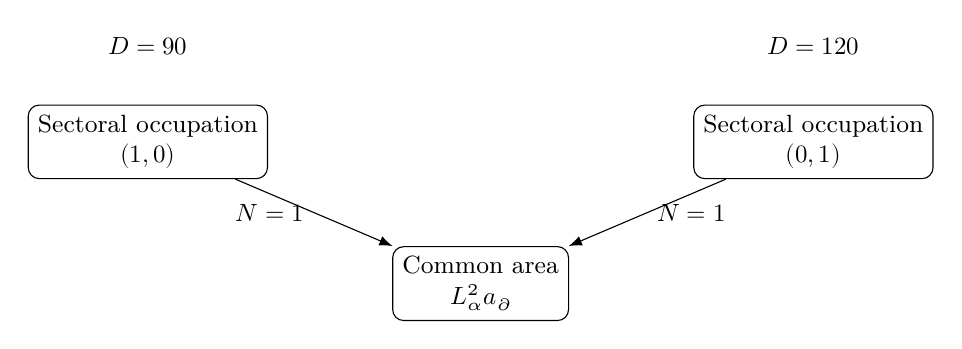
\begin{tikzpicture}[>=Latex,every node/.style={font=\small},node distance=15mm]
\node[draw,rounded corners,align=center] (a) {Sectoral occupation\\$(1,0)$};
\node[draw,rounded corners,align=center,right=54mm of a] (b) {Sectoral occupation\\$(0,1)$};
\node[draw,rounded corners,align=center] (n) at ($(a)!0.5!(b)+(0,-1.8)$)
 {Common area\\$L_\alpha^2a_\partial$};
\draw[->] (a)--node[left] {$N=1$}(n);
\draw[->] (b)--node[right] {$N=1$}(n);
\node[above=5mm of a] {$D=90$};
\node[above=5mm of b] {$D=120$};
\end{tikzpicture}
\caption{Equality of area preserves total occupation. Incidence
weighting distinguishes the two compositions; their joint reading allows
the occupations of both sectors to be reconstructed.}
\label{rev4:ae:figura}
\end{figure}

\subsection{Reduced state, purification and entanglement entropy}

The informational interpretation requires the state to be fixed. For
finite \(\Delta\in\mathbb R\), with the normalization of the modular
parameter of the sectoral construction, we define
\begin{equation}
 x_m=e^{-m\Delta},\qquad z_m=1+x_m+x_m^2,
 \qquad Z=z_{90}^{18}z_{120}^{18},
 \qquad \rho_A(\Delta)=Z^{-1}e^{-\Delta D}.
 \label{rev4:ae:rho}
\end{equation}
The sum of commuting occupations and the tensor decomposition prove
the expression for \(Z\). All eigenvalues of \(\rho_A\) are
strictly positive for finite real \(\Delta\). Its modular
Hamiltonian, denoted by \(K_A\) to distinguish it from the arithmetic record
\(K\), is
\begin{equation}
 K_A=-\log\rho_A=(\log Z)I+\Delta D.
 \label{rev4:ae:modular}
\end{equation}
This operator characterizes the spectral distribution of the reduced state.
The time-evolution generator is defined in the dynamical development
with its own parameters and domain. For \(\Delta\ne0\), with
\(\Delta\) and the normalization known, the pair
\((\widehat{\mathcal A},K_A)\) recovers \((N,D)\) and, through
\eqref{rev4:ae:inversa}, both occupations. For \(\Delta=0\),
the state is uniform and \(K_A=36\log3\,I\).

We construct the bipartition explicitly. Let \(\mathscr H_{\bar A}\)
be a copy of \(\mathscr H_A\), with the conjugate bases fixed. For
a link of weight \(w\), the vector
\[
 |\operatorname{TFD}(w)\rangle
 =\frac1{\sqrt{1+e^{-w}+e^{-2w}}}
 \sum_{n=0}^{2}e^{-wn/2}|n\rangle_A\otimes|n\rangle_{\bar A}
\]
has norm one. The pure state
\begin{equation}
 |\Psi_\Delta\rangle
 =|\operatorname{TFD}(90\Delta)\rangle^{\otimes18}
  \otimes|\operatorname{TFD}(120\Delta)\rangle^{\otimes18}
 \label{rev4:ae:tfd}
\end{equation}
determines the bipartition \(A\mid\bar A\).

\begin{proposition}[Sectoral reduction and entropy of the purification]
\label{rev4:ae:entropia}
The partial trace of \(|\Psi_\Delta\rangle\langle\Psi_\Delta|\)
over \(\mathscr H_{\bar A}\) is \(\rho_A(\Delta)\). Defining
\[
 f_m=\frac{x_m+2x_m^2}{z_m},
 \qquad s(\Delta)=-\Tr(\rho_A(\Delta)\log\rho_A(\Delta)),
\]
we have
\begin{align}
 \langle N\rangle_\Delta&=18(f_{90}+f_{120}),\\
 \langle D\rangle_\Delta&=18(90f_{90}+120f_{120}),\\
 \langle\widehat{\mathcal A}\rangle_\Delta
 &=18L_\alpha^2a_\partial(f_{90}+f_{120}),\\
 s(\Delta)&=18\log z_{90}+18\log z_{120}
             +\Delta\langle D\rangle_\Delta.
 \label{rev4:ae:entropia-formula}
\end{align}
The last expression is the entanglement entropy of the
purification \eqref{rev4:ae:tfd}, in dimensionless units.
\end{proposition}
\begin{proof}
In the partial trace of a link, the orthogonality of
\(|n\rangle_{\bar A}\) eliminates terms with distinct indices and
leaves the weights \((1,x_m,x_m^2)/z_m\). The partial trace of a tensor
product is the product of the partial traces; this yields
\eqref{rev4:ae:rho}. The first moment of each link is \(f_m\).
Additivity of the number operators gives the first three identities.
The last follows by substituting \eqref{rev4:ae:modular} into
\(s=\Tr(\rho_AK_A)\). The coefficients of the preceding construction
are Schmidt coefficients of the stated bipartition, so
this entropy coincides with its entanglement entropy.
\end{proof}

The maximum entropy of this space is \(36\log3\), attained at
\(\Delta=0\). The quantity \(36\log3-s(\Delta)\) is the
relative entropy of \(\rho_A(\Delta)\) with respect to
\(I/3^{36}\). Incidence fixes the sectors and their multiplicities;
the state parameter fixes the probabilities; the dimensional chart
converts occupation into area. The physical identification of
\(\mathscr H_{\bar A}\) preserves the bipartition and the algebra of
observables just specified.

\subsection{Finite modular identity and transport of geometric information}

Fix the reference state \(\rho_0=\rho_A(\Delta_0)\), with
finite real \(\Delta_0\), and hold
\(\Delta_0,a_\partial,L_\alpha\) constant. The normalized sectoral
areas \(\mathcal A_m^{\rm n}=a_\partial N_m\) satisfy
\begin{equation}
 K_0=-\log\rho_0=c_0I+
 \beta_{90}\mathcal A_{90}^{\rm n}
 +\beta_{120}\mathcal A_{120}^{\rm n},
 \qquad c_0=\log Z(\Delta_0),\qquad
 \beta_m=\frac{m\Delta_0}{a_\partial}.
 \label{rev4:ae:betas}
\end{equation}
The relation \(\beta_{120}=\tfrac43\beta_{90}\) preserves the incidence
ratio. For \(\Delta_0\ne0\), the ratio of the two coefficients
is defined and equals \(4/3\).

\begin{theorem}[Finite identity of area and relative information]
\label{rev4:ae:ley-finita}
For every normalized state \(\sigma\) of \(\mathscr H_A\), let
\(\delta_\sigma\langle B\rangle=\Tr[(\sigma-\rho_0)B]\).
Then
\begin{equation}
 s(\sigma)-s(\rho_0)
 =\sum_{m\in\{90,120\}}\beta_m
       \delta_\sigma\langle\mathcal A_m^{\rm n}\rangle
   -D(\sigma\Vert\rho_0),
 \label{rev4:ae:ley-finita-formula}
\end{equation}
where \(D(\sigma\Vert\rho_0)=
\Tr[\sigma(\log\sigma-\log\rho_0)]\) is finite and nonnegative,
with the convention \(0\log0=0\).
\end{theorem}
\begin{proof}
The definition yields
\(D(\sigma\Vert\rho_0)=-s(\sigma)+\Tr(\sigma K_0)\),
while \(s(\rho_0)=\Tr(\rho_0K_0)\). Subtracting the identities
and substituting \eqref{rev4:ae:betas} proves
\eqref{rev4:ae:ley-finita-formula}; the scalar term vanishes
by normalization of the traces. For positivity, let \(p_i\)
and \(u_i\) be the eigenvalues and eigenvectors of \(\sigma\), and
\(q_j>0,v_j\) those of \(\rho_0\). With
\(r_i=\langle u_i,\rho_0u_i\rangle\), concavity of
\(\log\) gives
\(\langle u_i,\log\rho_0u_i\rangle\le\log r_i\).
Thus, \(D(\sigma\Vert\rho_0)\ge\sum_i p_i\log(p_i/r_i)\ge0\),
by convexity of \(t\log t\), since \(\sum_i r_i=1\).
Full rank of \(\rho_0\) guarantees finiteness.
\end{proof}

Its infinitesimal version keeps the reference state fixed. If
\(\sigma(\varepsilon)\) is differentiable, normalized and
\(\sigma(0)=\rho_0\), then
\[
 \left.\frac{\dd s(\sigma(\varepsilon))}{\dd\varepsilon}\right|_0
 =\sum_m\beta_m
  \left.\frac{\dd\langle\mathcal A_m^{\rm n}\rangle_{
                          \sigma(\varepsilon)}}{\dd\varepsilon}\right|_0.
\]
Indeed, the derivative of the trace of \(-\sigma\log\sigma\) is
\(-\Tr[\dot\sigma(\log\rho_0+I)]\); normalization eliminates
\(\Tr\dot\sigma\) and substitution of \(K_0\) gives the formula.
The finite identity adds the exact relative-entropy correction
to that tangent response. The coefficients of the physical areas are
\(\beta_m/L_\alpha^2\), preserving the same dimensional chart.

Composition with the Grassmannian representation finally specifies
what information is preserved. In
\(\mathcal F(K,\xi)=([B(K)],Q,\xi)\), the additional coordinates
\(\xi\) retain the regional magnitudes, angular orientation,
marked inclusion, sector identification, occupation
basis, parameter \(\Delta\) and relevant area unit.
The inverse of Proposition~\ref{prop:compat-inversa-marcada}
recovers \(K\); the other conditions are preserved through their
markings. By Theorem~\ref{thm:compat-algebra-lectores}, composition
with that inverse transports \(\gamma_{\rm HMT}\),
\(\widehat{\mathcal A}\), \(\rho_A\), \(K_A\) and their evaluations
on the stated domain. Changes of chart of the same marked point
preserve these objects, and refinements preserve the inherited
evaluations when they maintain the same sectoral data.

This articulation preserves three distinguishable levels of information.
The marked positive representation recovers the record with the retained
data; the area--modular-Hamiltonian pair recovers the two
occupations under the conditions of \eqref{rev4:ae:modular}; the
purification determines the entanglement of a specific bipartition.
Information loss in a projection is computed through its fibers:
area identifies occupations with equal sums, while the joint
reading distinguishes their composition and preserves the remaining microscopic
degeneracy. The link between geometry and information is thus expressed
by verifiable maps and identities on the same construction.
\subsection{Naturality of the scale and operator-valued canonical forms}
\label{rev5:naturalidad-areal}

The generated length makes the compatibility between the positive
realisation, the area operator, and sectorial information explicit.
The marked representation \(\mathcal F(K,\xi)\) retains,
among the relevant data in \(\xi\), the resolution
\(\Omega\), its projectors, the transported return, and the section
\(L_*\). The generated regional coordinates, the action, and the constitutive
channels retain their preceding genealogy. The marked inverse
therefore recovers every argument of
\eqref{rev5:longitud-generada} and \eqref{rev5:G-area}.
In particular, the previously constructed geometric reader of
\(\alpha^{\mathrm{geom}}\) determines the expressions
\[
 L_\alpha^{\mathrm{geom}}
 =L_*(\alpha^{\mathrm{geom}})^{16}\frac{5759}{23040},
 \qquad
 G^{\mathrm{geom}}
 =\frac{(c^{\mathrm{geom}})^3
 (L_\alpha^{\mathrm{geom}})^2}{\hbar_{\rm ret}^{\mathrm{geom}}}.
\]
The speed and action readers are obtained by the same composition
with the marked inverse. These expressions retain the return data
and the radial reference section.

\begin{corollary}[Preservation under changes of chart and inherited refinement]
\label{rev5:conservacion}
Positive changes of chart preserving the marked point, and
refinements recovering the initial record, preserve
\(L_\alpha\), \(G\), \(\gamma_{\rm HMT}\), and
\(\widehat{\mathcal A}=L_\alpha^2a_\partial N\), provided
they also transport the declared sectorial and dimensional data.
The normalised spectrum
\(\widehat{\mathcal A}/L_\alpha^2=a_\partial N\), its
multiplicities, and the state \(\rho_A(\Delta)\) remain unchanged.
\end{corollary}
\begin{proof}
Theorem~\ref{thm:compat-algebra-lectores} transports each reader
by composition with the inverse. Mutations of the same point
reconstruct the same record. Under inherited refinement, summing
the subdivided separations reconstructs each initial coordinate.
Tensor extension of the inscription preserves \(r_\Omega\),
while its remaining arguments are fixed by the markings.
Substitution therefore preserves the length, the gravitational
coefficient, and the area operator. The occupation projectors
preserve the multiplicity polynomial \((1+z+z^2)^{36}\) and
the normalised expression of the state.
\end{proof}

The inherited refinement considered here retains the same space
of thirty-six boundary links. An extension introducing a different
physical boundary space requires specified intertwining maps for
\(N_{90}\) and \(N_{120}\), together with the transport of the
declared sectorial data.

Let \(P\) now be a rank-one polytope constructed in this manuscript,
with an oriented subdivision \(P=\bigcup_\sigma P_\sigma\)
having the same support, multiplicity one, and compatible faces.
The same sectorial fibre \(\mathscr H_A\) is fixed over all
its cells. The operator-valued top-degree form with the
dimension of area is defined by
\[
 \boldsymbol\Omega^{\mathcal A}_P
 =\widehat{\mathcal A}\otimes\Omega_P.
\]
Here \(\widehat{\mathcal A}\) is constant with respect to the
differential coordinates of the polytope: it is determined by the
fixed HMT state, whereas \(\Omega_P\) describes its geometric support.
The coefficient \(\widehat{\mathcal A}\) is positive semidefinite.
Its component in the vacuum sector \(N=0\) vanishes. On an
eigenspace with occupation \(n>0\), division by
\(nL_\alpha^2a_\partial\) recovers the canonical form
\(\Omega_P\) multiplied by the identity on that eigenspace.

\begin{proposition}[Areal additivity and boundary residues]
\label{rev5:forma-areal}
In the common sectorial trivialisation,
\begin{equation}
 \boldsymbol\Omega^{\mathcal A}_P
 =\sum_\sigma\widehat{\mathcal A}\otimes\Omega_{P_\sigma},
 \qquad
 \operatorname{Res}_F\boldsymbol\Omega^{\mathcal A}_P
 =\widehat{\mathcal A}\otimes\Omega_F.
\end{equation}
These identities persist under successive subdivisions and
iterated residues. For a fixed state \(\rho\), taking the trace
gives \(\Tr(\rho\widehat{\mathcal A})\Omega_P\) and preserves
the same scalar identities.
\end{proposition}
\begin{proof}
The operator space of \(\mathscr H_A\) is finite-dimensional.
In any basis, the assertion is the additivity identity for
canonical forms multiplied by each constant matrix entry of
\(\widehat{\mathcal A}\). Both residue and trace are linear.
Cancellation at interior facets retains their orientations and
the same operator entry on both sides. Iteration applies these
operations to each subdivision and each flag of faces.
\end{proof}

If distinct cells carry regular operator-valued coefficients
\(A_\sigma\), the defect of a pair along its common face is
\((A_\sigma|_F-A_\tau|_F)\otimes\Omega_F\).
Equality of the operator-valued restrictions to the boundary
provides the gluing condition, under the simple-pole hypotheses
of Theorem~\ref{thm:compat-pegado}. The global sum must also retain
every contribution along each ambient divisor and the control
of exterior poles. Dimensional normalisation, residue cancellation,
and coverage of the support therefore have distinct and
compatible criteria.

The finite modular identity likewise admits a direct expression
in physical areas \(\mathcal A_m=L_\alpha^2a_\partial N_m\):
\begin{equation}
 s(\sigma)-s(\rho_0)
 =\sum_{m=90,120}\frac{m\Delta_0}{L_\alpha^2a_\partial}
   \Tr[(\sigma-\rho_0)\mathcal A_m]
  -D(\sigma\Vert\rho_0).
 \label{rev5:modular-fisica}
\end{equation}
This is \eqref{rev4:ae:ley-finita-formula} after substitution
of the constructed length. The angular factor \(a_0\), contained
in \(a_\partial=\gamma_{\rm HMT}a_0\), is retained in full.
When dimensional sections satisfying \(L'_\alpha=sL_\alpha\)
are compared while preserving the same state and the same
dimensionless data, areas are multiplied by \(s^2\) and their
modular coefficients by \(s^{-2}\). Entropy and relative entropy
remain unchanged. This comparison of sections does not constitute
a second solution for the same fixed longitudinal data.

For a spherical horizon of radius \(R_h=L_\alpha\zeta_h\),
the geometric area is \(4\pi_{\rm HMT}L_\alpha^2\zeta_h^2\).
Its identification with the expectation of the sectorial operator,
when required for the same cross-section, imposes the explicit
condition
\[
 a_\partial\Tr(\rho N)=4\pi_{\rm HMT}\zeta_h^2.
\]
The horizon geometry and the boundary state must satisfy this
relation through their respective constructions. The factor
\(\zeta_h\) characterises that horizon; the longitudinal scale
of the coupling remains \(L_\alpha\).


\begingroup
\setlength{\intextsep}{3pt}
\begin{figure}[H]
\centering
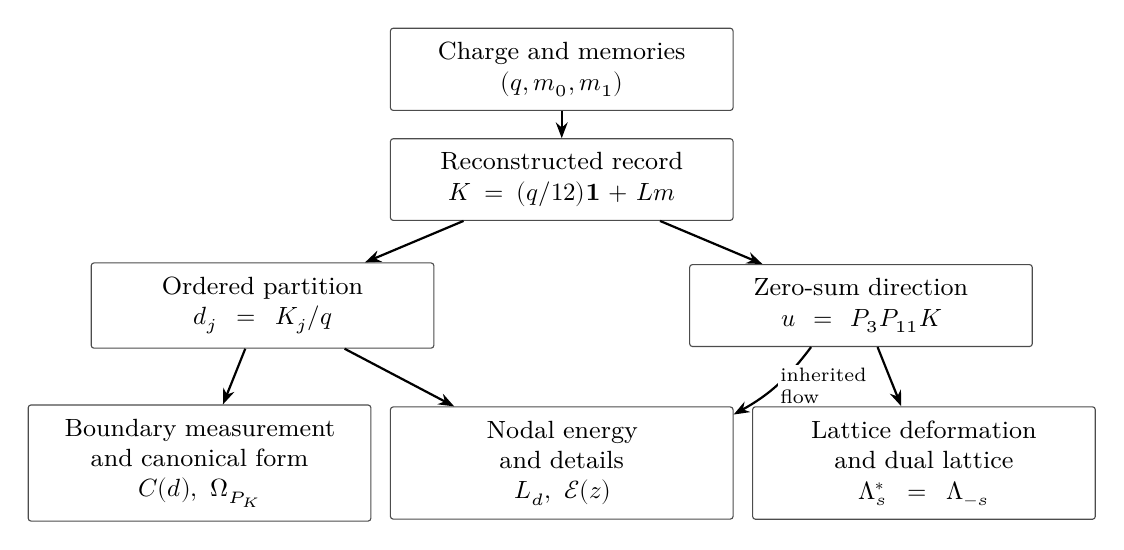
\begin{tikzpicture}[
 box/.style={draw=black!70,rounded corners=1pt,align=center,
             font=\small,inner sep=5pt,text width=40mm},
 arrow/.style={-{Stealth[length=2mm]},thick}]
\node[box] (memory) at (0,0) {Charge and memories\\\((q,m_0,m_1)\)};
\node[box] (register) at (0,-1.4) {Reconstructed record\\\(K=(q/12)\mathbf1+Lm\)};
\node[box] (weights) at (-3.8,-3.0) {Ordered partition\\\(d_j=K_j/q\)};
\node[box] (direction) at (3.8,-3.0) {Zero-sum direction\\\(u=P_3P_{11}K\)};
\node[box] (geometry) at (-4.6,-5.0) {Boundary measurement\\and canonical form\\\(C(d),\ \Omega_{P_K}\)};
\node[box] (energy) at (0,-5.0) {Nodal energy\\and details\\\(L_d,\ \mathcal E(z)\)};
\node[box] (lattice) at (4.6,-5.0) {Lattice deformation\\and dual lattice\\\(\Lambda_s^*=\Lambda_{-s}\)};
\draw[arrow] (memory)--(register);
\draw[arrow] (register)--(weights);
\draw[arrow] (register)--(direction);
\draw[arrow] (weights)--(geometry);
\draw[arrow] (weights)--(energy);
\draw[arrow] (direction)--(lattice);
\draw[arrow] (direction) to[bend left=12] node[right,font=\scriptsize,align=left,fill=white,inner sep=1pt]{inherited\\flow} (energy);
\end{tikzpicture}
\caption{Subsequent realizations of the recoverable record. The interval
branch determines path minors, the polygon's canonical form
and the nodal Laplacian. The algebraic direction determines the
interval flow and, together with the marked lattice realization, the
twenty-four-dimensional dual collection. Each arrow preserves the domain
and hypotheses of its construction; the lower codomains are
distinct.}
\label{fig:multimorphology}
\end{figure}
\endgroup


\clearpage
\part{Gauge realization, refinement and spectral gap}
\section{Positivities, physical spaces, and spectral transport}
Positive geometry and gauge theory receive distinct structures from
the same genealogical process. The former realizes the weights and their
incidences through ordered minors, cells, and canonical forms.
The latter preserves gauge incidence, holonomy,
representations, routes, and memory within a compatible measure.
Its form of positivity relevant to physical reconstruction is
reflection positivity. The conceptual connection acquires mathematical
content when the maps producing each form are preserved.

In the geometric part, it has been proved that subdividing a cell
preserves its canonical form through cancellation of interior poles.
For nodal energies, Schur reduction preserves an effective
form and records the detail. In the gauge part, refinement
compatibility must also preserve the vacuum, the invariant subspace,
the generator, and the spectral witness. This is the chain developed
below: arithmetic--geometric scale, common measure, semigroup,
physical projection, refinement, and continuous reconstruction.

The norm of a vector, the positivity of a moment matrix, and the
existence of a Hamiltonian gap have different domains.
A congruence with an invertible factor preserves the positivity and
inertia of a form; an isometric intertwining of the generator, together
with its domain, transports its realization onto the reduced image of the
inclusion. The uniform bound and the persistent witness then determine the
limiting gap. The development therefore keeps explicit the
inclusions and semigroup identities that justify passage to the
limit. The gap scale originates in areal--volumetric incidence
and its declared dimensional unit.

The following sections bring together the projective construction and its
subsequent development depending on the coupling \(g\). The initial
comparisons with a Gibbs parametrization are subsequently completed through
the explicit action, measure, and transport. The expository order
preserves the proofs of the process and places the complete formulation
after its dependencies. The four reflections correspond to the four
Euclidean directions of the reconstruction. The development assembled here
concerns this gauge theory and its gap, with the compact,
connected, simple group declared in the theorems.

The planar supersymmetric sector in which amplitudes are studied through
amplituhedra retains a specific physical question. Connecting it with
the present realization requires the supercharge operators, their
domains, and the corresponding representation. The dimension four of the
Euclidean chart and the difference four of the modular block remain
previously defined results of their respective operators.

\section{Areal--volumetric transition and spectral scale}
\label{sec:ym-areal-volumetric-scale}

The constant determining the gauge semigroup is obtained before the
Hamiltonian is introduced. Its origin combines two independent readers of the same
genealogical state: the return frequency yielding
\(\pi_{\rm HMT}\) and the stationary distribution of the two
areal--volumetric sheets.

\subsection{Dynamics of the two sheets}

Let
\begin{equation}
 F_{\rm av}=\begin{pmatrix}0&1\\1&1\end{pmatrix},
 \qquad e_{\rm ar}=\binom10,
 \qquad e_{\rm vol}=\binom01.
 \label{eq:ym-av-transition-matrix}
\end{equation}
The Fibonacci recurrence gives, by induction,
\begin{equation}
 F_{\rm av}^{n}
 =\begin{pmatrix}F_{n-1}&F_n\\F_n&F_{n+1}\end{pmatrix}.
 \label{eq:ym-av-fibonacci-powers}
\end{equation}
The Perron vector is proportional to \((1,\varphi)\). Since
\(F_{\rm av}\) is symmetric, the Parry measure assigns the two sheets
weights proportional to \((1,\varphi^2)\), and hence
\begin{equation}
 \frac{\mu_{\rm ar}}{\mu_{\rm vol}}=\varphi^{-2},
 \qquad
 \mu_{\rm vol}=\frac{\varphi^2}{1+\varphi^2}.
 \label{eq:ym-av-parry-weights}
\end{equation}
Here \(\mu_{\rm vol}\) is a dimensionless frequency character; it does not
denote a volume of dimension \(L^4\).

The regional reader of \(\pi\) is introduced exactly once through
\begin{equation}
 D_\pi
 =\pi_{\rm HMT}|e_{\rm ar}\rangle\langle e_{\rm ar}|
  +|e_{\rm vol}\rangle\langle e_{\rm vol}|.
 \label{eq:ym-pi-regional-reader}
\end{equation}
The ratio obtained at depth \(n\) is
\begin{equation}
 \Theta_n
 :=\frac{\langle e_{\rm ar},D_\pi F_{\rm av}^{n}e_{\rm ar}\rangle}
 {\langle e_{\rm vol},F_{\rm av}^{n}e_{\rm vol}\rangle}
 =\pi_{\rm HMT}\frac{F_{n-1}}{F_{n+1}}
 \longrightarrow
 r_{\rm av}:=\frac{\pi_{\rm HMT}}{\varphi_{\rm HMT}^{2}}.
 \label{eq:ym-target-free-av-limit}
\end{equation}
The matrix, route, and quotient are fixed before consulting a mass
gap or a gauge-theory parameter. At the native depth \(n=108\),
\begin{equation}
 F_{107}=10284720757613717413913,
 \qquad
 F_{109}=26925748508234281076009,
 \label{eq:ym-fibonacci-107-109}
\end{equation}
and
\begin{equation}
 \left|\Theta_{108}
 -\frac{\pi_{\rm HMT}}{\varphi_{\rm HMT}^{2}}\right|
 <2\cdot10^{-45}.
 \label{eq:ym-av-depth-108-error}
\end{equation}

\subsection{Dimensional transduction}

Let \(\ell_0\) be the length unit of the dimensional reader. The inverse
length scale and the parameter of a slab of thickness \(a_m\) are
\begin{equation}
 \kappa_{\rm av}
 :=\frac{\mu_{\rm vol}}{\ell_0}
 \left(\frac{\pi_{\rm HMT}}{\varphi_{\rm HMT}^{2}}-1\right)>0,
 \qquad
 q_m:=e^{-3a_m\kappa_{\rm av}}.
 \label{eq:ym-dimensional-gap-scale}
\end{equation}
Thus \([\kappa_{\rm av}]=L^{-1}\), and the energy gap is
\begin{equation}
 \Delta_E=3\hbar c\,\kappa_{\rm av};
 \label{eq:ym-energy-gap-units}
\end{equation}
in units \(\hbar=c=1\), this is written as \(\Delta_E=3\kappa_{\rm av}\).
The electronic memory \(\Delta_4\) belongs to a different domain and a different
reader; it does not enter \eqref{eq:ym-dimensional-gap-scale}.

In the semigroups of the following sections, \(t,s,a_m\) are
Euclidean lengths and the generators \(D\) and \(H^{\rm ov}\) have
dimension \(L^{-1}\). The energy Hamiltonian is
\(H_E=\hbar_{\rm int}c_{\rm int}D\). If
\(\tau=t/c_{\rm int}\), then
\[
 e^{-tD}=e^{-\tau H_E/\hbar_{\rm int}},\qquad
 \Delta=3\kappa_{\rm av},\quad
 \Delta_E=\hbar_{\rm int}c_{\rm int}\Delta,\quad
 m_{\rm gap}=\frac{\hbar_{\rm int}\Delta}{c_{\rm int}}.
\]
The same gap is thus expressed, respectively, as inverse
length, energy, and mass in the declared dimensional chart.

Since \(a_m=9a_{m+1}\), the definition immediately gives
\begin{equation}
 q_{m+1}^{9}=q_m.
 \label{eq:ym-nonadic-gap-root}
\end{equation}
This identity is the nonadic root that will transport the same semigroup and
the same spectral scale through every refinement.

\section[Euclidean Yang--Mills gauge process in dimension 4]{Projective
construction of a Euclidean Yang--Mills gauge process, Osterwalder--Schrader
reconstruction, and collective gap in dimension \(4\)}


\noindent The specialization of the enriched nonadic dynamics,
constructed in the preceding sections, is
\[
 (\widehat X_\infty,\Gamma_9)
 \xrightarrow{\ \mathcal R_{\rm YM}\ }
 (\mu_m,T_m,H_m,\Omega_m)
 \longrightarrow(\mu_\infty,\mathrm{OS},E(4))
 \longrightarrow\operatorname{gap}(H_{\rm phys})>0.
\]
The clover reader yielding \(F^2\) recognizes curvature on this same
projective process; it does not construct \(\mu_m\) retrospectively. The gauge
theory, OS reconstruction, simple vacuum, and gap are already determined
by this chain. The identity
\eqref{eq:amp-ym-identidad-accion-requerida} subsequently compares an
optional parametrization by \(g_R\); it is a non-governing check, not a
condition for identifying the constructed Yang--Mills theory.

\subsection*{Gauge object and refinement domain}

Let \(G\) be a compact, connected, simple Lie group. For each
\(m\geq0\), consider the Euclidean lattice
\begin{equation}\label{eq:realizaciones-ym-red}
 \Lambda_m=a_m\mathbb Z^4,
 \qquad a_{m+1}=\frac{a_m}{9}.
\end{equation}
The cylindrical gauge algebra is generated by link variables in \(G\),
representation intertwining operators, and the enriched coordinates
of color,
orientation, holonomy, fusion carry, route, and memory. Let \(\mu_m\) be the
common invariant measure and let
\[
 \mathcal H_m=L^2(\mathcal A_m,\mu_m)^{\rm gauge}.
\]
The constant vector \(\Omega_m\) defines
\begin{equation}\label{eq:realizaciones-ym-proyectores}
 P_{\Omega_m}=|\Omega_m\rangle\langle\Omega_m|,
 \qquad Q_m^{\rm phys}=I-P_{\Omega_m}.
\end{equation}
The second projector is the physical complement of the vacuum; it is not identified
with a residual used solely to organize the renormalization
scale.

The update circuit is local:
\begin{equation}\label{eq:realizaciones-ym-circuito}
 K_m^{\rm loc}
 =\prod_{r=1}^{9\cdot81}
   \prod_{B\in\mathcal B_{m,r}}K_{m,B}.
\end{equation}
The partition \(\{\mathcal B_{m,r}\}_r\) enumerates each coordinate exactly once; the circuit
factors will be identified below with the semigroup of their conditional
expectations, not with nine independent dynamics.
Blocks of the same color have disjoint supports, and the physical diameter
of each support is uniformly bounded as \(m\) varies. This locality
is part of the object, so that refinement does not turn an
elementary update into an instantaneously global operation.

Let \(T_m\) be the transfer induced by
\eqref{eq:realizaciones-ym-circuito}. The isometric inclusions
\(J_m:\mathcal H_m\to\mathcal H_{m+1}\) preserve ancestry,
representation, orientation, carry, and memory. For the four Euclidean
reflections \(\Theta_{\nu,m}\), \(\nu=1,\ldots,4\), one has
\begin{equation}\label{eq:realizaciones-ym-entrelazamiento}
 (T_{m+1})^9J_m=J_mT_m,
 \qquad
 \Theta_{\nu,m+1}J_m=J_m\Theta_{\nu,m}
 \quad(\nu=1,\ldots,4).
\end{equation}
The four directions therefore belong to the same refinement, the same
measure, and the same dynamics.

\subsection*{Common semigroup, relative corona, and four reflection forms}

In the triangular chart of the complete state, let \(E_{m,c}\) be the commuting
orthogonal conditional expectations associated with independent
coordinates. The positive overlap generator is first constructed at
a seed level \(m_0\):
\begin{equation}\label{eq:realizaciones-ym-generador}
 \widehat H_{m_0}^{\rm ov}
 =3\kappa_{\rm av}
  \sum_{c\in\mathcal I_{m_0}^{\rm seed}}(I-E_{m_0,c}),
\end{equation}
and is extended by
\begin{equation}\label{eq:realizaciones-ym-generador-refinado}
 \begin{aligned}
 \widehat H_{m+1}^{\rm ov}
 &=\widehat\Gamma_m^*
   \bigl(\widehat H_m^{\rm ov}\otimes I+
         I\otimes\widehat H_{m+1}^{\rm det}\bigr)
   \widehat\Gamma_m,\\
 \widehat H_{m+1}^{\rm det}
 &=3\kappa_{\rm av}
   \sum_{\iota\in\mathcal I_{m+1/m}^{\rm det}}
   (I-E_{m+1,\iota}^{\rm det}),
 \end{aligned}
\end{equation}
where
\begin{equation}\label{eq:realizaciones-ym-kappa}
 \kappa_{\rm av}
 =\frac{\mu_{\rm vol}}{\ell_0}
  \left(\frac{\pi_{\rm HMT}}{\varphi_{\rm HMT}^{\,2}}-1\right)>0.
\end{equation}
The volumetric frequency \(\mu_{\rm vol}\) is dimensionless; the dimension
comes from \(\ell_0\).

The semigroup, the transfer over one physical step, and their scale
compatibility are defined with explicit types:
\begin{equation}\label{eq:realizaciones-ym-semigrupo}
 \widehat K_{m,t}^{\rm ov}=e^{-t\widehat H_m^{\rm ov}},
 \qquad
 \widehat T_m=\widehat K_{m,a_m}^{\rm ov},
 \qquad a_{m+1}=a_m/9,
\end{equation}
Since the partition enumerates each coordinate exactly once and the conditional
expectations of its blocks commute, for each block and for the complete
circuit one obtains
\begin{equation}\label{eq:realizaciones-ym-circuito-semigrupo}
 K_{m,B}=e^{-3\kappa_{\rm av}a_m(I-E_{m,B})},
 \qquad
 K_m^{\rm loc}=e^{-a_m\widehat H_m^{\rm ov}}=\widehat T_m.
\end{equation}
\begin{equation}\label{eq:realizaciones-ym-semigrupo-entrelazado}
 \widehat H_{m+1}^{\rm ov}\widehat J_m
 =\widehat J_m\widehat H_m^{\rm ov},
 \qquad
 (\widehat T_{m+1})^9\widehat J_m
 =\widehat J_m\widehat T_m.
\end{equation}
Thus, the ninth power is compared through \(\widehat J_m\); operators
acting on different Hilbert spaces are not equated.

The common eight-face measure originates in this same reversible kernel:
\begin{equation}\label{eq:realizaciones-ym-medida-ocho}
 \widehat\Omega_m^{(8)}(dy_1\cdots dy_8)
 =\int\widehat\mu_m^{\rm ov}(dz)
   \prod_{r=1}^{8}
   \widehat K_{m,a_m/2}^{\rm ov}(z,dy_r).
\end{equation}
For each reflection \(\nu=1,\ldots,4\) and every cylindrical observable \(F\)
in the positive half-space,
\begin{equation}\label{eq:realizaciones-ym-os}
 \int\overline{F(\Theta_{\nu,m}y)}F(y)\,
 d\widehat\Omega_m^{(8)}
 =\|\widehat{\mathcal B}_{m,\nu}F\|^2\geq0,
\end{equation}
and the marginal on opposite faces gives the connecting identity
\begin{equation}\label{eq:realizaciones-ym-os-transferencia}
 \widehat T_{m,\nu}^{\rm OS}
 =\widehat K_{m,a_m}^{\rm ov}
 =e^{-a_m\widehat H_m^{\rm ov}}
 =\widehat T_m,
 \qquad \nu=1,\ldots,4.
\end{equation}
The four reflections therefore yield the same
transfer--measure pair.

\subsection*{Cellular persistence of the terminal and exact gap}

Let
\[
 K_9=C_*(Q_{9,3};\mathbb Z),\qquad
 K_{10}=C_*(Q_{10,3};\mathbb Z).
\]
The relative corona has dimensions
\[
 C_*(Q_{10,3},Q_{9,3})=(271,756,702,217),
 \qquad 271+702=756+217=973.
\]
The inclusion \(j:K_9\to K_{10}\), cellular collapse
\(r:K_{10}\to K_9\), and integral homotopy \(H_{\rm cell}\) satisfy
\begin{equation}\label{eq:realizaciones-ym-sdr-corona}
 rj=I,\qquad
 \partial H_{\rm cell}+H_{\rm cell}\partial=I-jr,\qquad
 rH_{\rm cell}=0,\quad H_{\rm cell}j=0,\quad H_{\rm cell}^2=0.
\end{equation}
For every chain map
\(F:K_{10}\otimes V_{q=6}\to\mathcal T\), with
\(P=(jr)\otimes I_{q=6}\),
\begin{equation}\label{eq:realizaciones-ym-homotopia-terminal}
 F-FP
 =d_{\mathcal T}\bigl(F(H_{\rm cell}\otimes I)\bigr)
  +F(H_{\rm cell}\otimes I)(\partial\otimes I).
\end{equation}
The complete corona is thus null-homotopic, and the terminal \(FP\) remains
literally unchanged. The \(271\) vertices do not replace the edges, faces, and cubes
of the corona; nor is the three-dimensional cellular factor identified with the
physical gauge factor \(q=6\).

For each persistent coordinate \(c\), in the local chart
\(q=(q_1,\ldots,q_6)\in\mathbb F_3^6\), define the centered witness
\begin{equation}\label{eq:realizaciones-ym-testigo-definicion}
 \bigcap_c\operatorname{Ran}E_{m,c}=\mathbb C\Omega_m,
 \qquad
 W_c(q)=\mathbf 1_{\{q_1+\cdots+q_6=0\}}-\frac13,
\end{equation}
where the sum in the indicator is taken in \(\mathbb F_3\). The Hoeffding
decomposition of the commuting expectations proves
\begin{equation}\label{eq:realizaciones-ym-gap-finito}
 \ker\widehat H_m^{\rm ov}=\mathbb C\Omega_m,
 \qquad
 \widehat H_m^{\rm ov}\succeq
 3\kappa_{\rm av}(I-P_{\Omega_m}).
\end{equation}
Equality does not follow merely from the triviality of the kernel: each nonconstant
sector of the decomposition receives at least one projector
\(I-E_{m,c}\), and by \eqref{eq:realizaciones-ym-generador} its minimum cost
is \(3\kappa_{\rm av}\). The explicit witness \(W_c\) satisfies
\begin{equation}\label{eq:realizaciones-ym-testigo-gap}
 \widehat H_m^{\rm ov}W_c=3\kappa_{\rm av}W_c,
 \qquad \|W_c\|^2=\frac29,
\end{equation}
so that the complement is nonempty and the gap is exactly
\(3\kappa_{\rm av}\).

The scale is expressed by
\begin{equation}\label{eq:realizaciones-ym-qm}
 q_m=e^{-3\kappa_{\rm av}a_m},
 \qquad q_{m+1}^{\,9}=q_m,
 \qquad -a_m^{-1}\log q_m=3\kappa_{\rm av}.
\end{equation}
Although \(q_m\to1\) under refinement, the spectral quotient per physical unit
remains constant. The cellular contraction
\eqref{eq:realizaciones-ym-homotopia-terminal} preserves the terminal; the
gap originates in the positive overlap generator and its Hoeffding
decomposition, not in acyclicity alone.

The inclusions in \eqref{eq:realizaciones-ym-semigrupo-entrelazado}
form the inductive limit
\begin{equation}\label{eq:realizaciones-ym-colimite}
 \mathcal H_\infty=\varinjlim(\mathcal H_m,\widehat J_m).
\end{equation}
On the algebraic inductive union, define the form
\begin{equation}\label{eq:realizaciones-ym-forma-limite}
 \mathfrak h_\infty[\widehat J_{m,\infty}\psi]
 :=\langle\psi,\widehat H_m^{\rm ov}\psi\rangle_{\mathcal H_m}.
\end{equation}
Intertwining of the generators makes this definition
independent of the representative. The form is positive and closable; its
closure determines the self-adjoint generator \(\widehat H_\infty^{\rm ov}\).
Compatibility of the forms transports
\begin{equation}\label{eq:realizaciones-ym-gap-forma-limite}
 \overline{\mathfrak h}_\infty[\psi]
 \geq3\kappa_{\rm av}
 \|(I-P_{\Omega_\infty})\psi\|^2,
\end{equation}
and the persistent vector
\(\widehat J_{m,\infty}W_c\) attains equality. Consequently, the
exact gap of the limiting generator is \(3\kappa_{\rm av}\).

\subsection*{Exact hypotheses and logical chain of the theorem}

The gauge realization uses:
\begin{enumerate}
 \item the compact, connected, simple group and the four-dimensional lattice
       \eqref{eq:realizaciones-ym-red};
 \item the local circuit \eqref{eq:realizaciones-ym-circuito}, with uniform
       physical diameter, and a common invariant measure;
 \item the isometric inclusions and the four reflections intertwined by
       \eqref{eq:realizaciones-ym-entrelazamiento} and
       \eqref{eq:realizaciones-ym-semigrupo-entrelazado};
 \item the four factorizations
       \eqref{eq:realizaciones-ym-os} and the exact connection
       \eqref{eq:realizaciones-ym-os-transferencia} on the same
       transfer--measure pair;
 \item the commuting-expectation generator
       \eqref{eq:realizaciones-ym-generador}--
       \eqref{eq:realizaciones-ym-generador-refinado} and its
       Hoeffding decomposition;
 \item the integral SDR of the corona and preservation of the terminal
       \eqref{eq:realizaciones-ym-sdr-corona}--
       \eqref{eq:realizaciones-ym-homotopia-terminal};
 \item the terminal \(P_{\Omega_m}\), the physical complement
       \(Q_m^{\rm phys}\), and the scaling law
       \eqref{eq:realizaciones-ym-qm};
 \item the inductive limit and the compatible closure of forms
       \eqref{eq:realizaciones-ym-colimite}--
       \eqref{eq:realizaciones-ym-gap-forma-limite};
 \item the internal action and velocity charts
       \(\hbar_{\rm int}\), \(c_{\rm int}\), used solely to express the
       mass dimension.
\end{enumerate}

\begin{theorem}[Local gauge theory with a simple vacuum and collective gap]
\label{thm:realizaciones-ym}
Under the preceding premises, the limit of the gauge collection is local and
reflection-positive in all four Euclidean directions. Its generator
has a simple vacuum and satisfies, in the gauge-invariant collective sector,
\begin{equation}\label{eq:realizaciones-ym-gap-limite}
 \Delta_{\rm YM}^{\rm HMT}=3\kappa_{\rm av}>0,
 \qquad
 m_{\rm gap}^{\rm HMT}
 =\frac{\hbar_{\rm int}}{c_{\rm int}}
  \Delta_{\rm YM}^{\rm HMT}>0.
\end{equation}
The gap belongs to the collective sector; it does not assign an elementary mass to the
gluon.
\end{theorem}

\begin{proof}
The uniform locality of the circuit preserves the net of local algebras. The
equalities \eqref{eq:realizaciones-ym-semigrupo-entrelazado} identify the
ninth power after applying the correct inclusion. The construction
\eqref{eq:realizaciones-ym-medida-ocho} uses this same semigroup on the eight
faces, and \eqref{eq:realizaciones-ym-os-transferencia} identifies its four
OS marginals with \(\widehat T_m\). Thus, the four positive forms
\eqref{eq:realizaciones-ym-os} are compatible in the limit and preserve a
single measure and a single dynamics.

The expectations in \eqref{eq:realizaciones-ym-generador} are orthogonal and
commuting. Their Hoeffding decomposition separates the constant mode from every
nonconstant sector: the former is \(\mathbb C\Omega_m\), whereas every
sector of the complement receives at least one factor \(I-E_{m,c}\) with weight
\(3\kappa_{\rm av}\). This proves
\eqref{eq:realizaciones-ym-gap-finito}. The witness
\eqref{eq:realizaciones-ym-testigo-gap} attains the bound, so it is not
merely a lower bound: it is the first nonzero energy.

The homotopy \eqref{eq:realizaciones-ym-homotopia-terminal} contracts the
cellular complement and leaves \(FP\) intact; the corona therefore introduces no
second vacuum and erases no carry. Isometric compatibility transports the
vacuum and its complement to the next level without mixing them with the scale
residual. The law
\eqref{eq:realizaciones-ym-qm} shows that the spectral quotient per physical
unit is exactly \(3\kappa_{\rm av}\) at every level. The forms
\eqref{eq:realizaciones-ym-forma-limite}--
\eqref{eq:realizaciones-ym-gap-forma-limite} transport the bound and the witness
to the self-adjoint limiting generator, so the gap remains exact.
Reconstruction by Osterwalder--Schrader
positivity identifies the Hamiltonian with the generator of this
same transfer, preserves the simple vacuum, and produces
\eqref{eq:realizaciones-ym-gap-limite}. The final dimensional chart transforms
the gap into the stated collective mass.
\end{proof}

\subsection*{Gauge compression and physical gap witness}

Let
\[
 \widehat{\mathscr H}_m
 :=L^2(\widehat X_m,\widehat\mu_m^{\rm ov})
\]
be the space of the complete material realization. In addition to the usual gauge
action on links and frames, each collar \(c\) carries the finite incidence
action
\begin{equation}\label{eq:amp-ym-accion-gauge-incidencia}
 q_c\longmapsto q_c+Bx_c,
 \qquad x_c\in\mathbb F_3^4,
\end{equation}

where the six rows of \(B\) are indexed by
\((01,02,03,12,13,23)\). The product of both actions preserves
\(\widehat\mu_m^{\rm ov}\). With \(\mathcal C_m\) denoting the finite set of
collars present at this level, write
\[
 \mathcal G_m^{\rm full}
 :=G^{V(\Lambda_m)}
   \times\prod_{c\in\mathcal C_m}\mathbb F_3^4.
\]
Its Haar average defines the orthogonal
projection
\begin{equation}\label{eq:amp-ym-proyeccion-fisica-haar}
 \mathbb P_m^{\rm phys}F
 :=\int_{\mathcal G_m^{\rm full}}F(g^{-1}\!\cdot\,)\,dg,
 \qquad
 \widehat{\mathscr H}_m^{\rm phys}
 :=\operatorname{Ran}\mathbb P_m^{\rm phys}.
\end{equation}
This is a compression onto the gauge subalgebra of the complete state; the
marginal forgetting the incidence coordinates is a different map and is not
confused with \(\mathbb P_m^{\rm phys}\).

\begin{lemma}[Reduction of the Hamiltonian to the physical subalgebra]
\label{lem:amp-ym-compresion-fisica}
The projection \(\mathbb P_m^{\rm phys}\) reduces the generator and its
semigroup. The refinement inclusions simultaneously reduce the
physical subalgebras:
\begin{equation}\label{eq:amp-ym-compresion-entrelazada}
 \begin{gathered}
 \relax
 [\mathbb P_m^{\rm phys},\widehat H_m^{\rm ov}]=0,
 \qquad
 [\mathbb P_m^{\rm phys},e^{-t\widehat H_m^{\rm ov}}]=0,\\
 \mathbb P_{m+1}^{\rm phys}\widehat J_m
 =\widehat J_m\mathbb P_m^{\rm phys},\qquad
 H_m^{\rm phys}
 :=\widehat H_m^{\rm ov}\big|_{\widehat{\mathscr H}_m^{\rm phys}},\\
 H_{m+1}^{\rm phys}\widehat J_m
 =\widehat J_mH_m^{\rm phys}.
 \end{gathered}
\end{equation}
\end{lemma}

\begin{proof}
The physical generator on links is gauge-equivariant by the
bi-invariance of Haar measure. In the product chart, \(E_{q_c}\) is uniform
expectation on \(\mathbb F_3^6\); invariance of the uniform measure under
the translations in \eqref{eq:amp-ym-accion-gauge-incidencia} implies that it commutes with
this action. Expectations on the marking subtails act on
disjoint factors. Thus every summand of
\[
 \widehat H_m^{\rm ov}
 =H_m^{\rm ov}\otimes I
 +3\kappa_{\rm av}\sum_c
 \bigl[(I-E_{q_c})+(I-E_{u_c^{\rm P}})\bigr]
\]
commutes with the average \eqref{eq:amp-ym-proyeccion-fisica-haar}. The
functional calculus gives commutation with the semigroup. Finally,
\(\widehat J_m\) preserves the ancestral factors and inserts the constant
in the new factors; averaging before or after this inclusion produces
the same function. This proves the four identities in
\eqref{eq:amp-ym-compresion-entrelazada}.
\end{proof}

\begin{lemma}[Nonzero intertwined gauge witness]
\label{lem:amp-ym-testigo-fisico-q6}
For every collar \(c\), the function
\begin{equation}\label{eq:amp-ym-testigo-fisico-def}
 W_c(q)
 :=\mathbf 1_{\{q_1+\cdots+q_6=0\}}-\frac13
\end{equation}
belongs to \(\widehat{\mathscr H}_m^{\rm phys}\), is nonzero, and satisfies
\begin{equation}\label{eq:amp-ym-testigo-fisico-momentos}
 \mathbb E W_c=0,\qquad
 \|W_c\|^2=\frac29,\qquad
 \mathbb E(W_c^3)=\frac2{27}.
\end{equation}
Moreover,
\begin{equation}\label{eq:amp-ym-testigo-fisico-gap}
 H_m^{\rm phys}W_c=3\kappa_{\rm av}W_c,\qquad
 H_{m+1}^{\rm phys}\widehat J_mW_c
 =3\kappa_{\rm av}\widehat J_mW_c.
\end{equation}
Consequently, the value \(3\kappa_{\rm av}\) belongs to the spectrum of the
physical restriction, not merely to that of a material dilation.
\end{lemma}

\begin{proof}
The gauge action on links acts on the first factor and fixes
\(W_c\). For the incidence action, each \(x_i\) appears in three of the
six coordinates, hence
\[
 \sum_{i<j}(Bx)_{ij}=3\sum_i x_i=0
 \quad\text{in }\mathbb F_3.
\]
The condition in \eqref{eq:amp-ym-testigo-fisico-def} is therefore
invariant; it is also invariant under permutations of the six incidences.
Thus \(\mathbb P_m^{\rm phys}W_c=W_c\).

Under the uniform measure, the sum of the six trits is uniform on
\(\mathbb F_3\). The function takes the value \(2/3\) with probability \(1/3\)
and \(-1/3\) with probability \(2/3\), giving
\eqref{eq:amp-ym-testigo-fisico-momentos}. The first summand of
\(\widehat H_m^{\rm ov}\) annihilates \(W_c\); for \(c'\ne c\),
\((I-E_{q_{c'}})W_c=0\), whereas
\(E_{q_c}W_c=0\). All marking expectations annihilate the
corresponding difference because \(W_c\) is constant on these subtails.
What remains is exactly
\(\widehat H_m^{\rm ov}W_c=3\kappa_{\rm av}W_c\). The first identity in
\eqref{eq:amp-ym-testigo-fisico-gap} follows from reduction; the second,
from the intertwining in \eqref{eq:amp-ym-compresion-entrelazada}.
\end{proof}

\subsection*{Gauge semigroup, vacuum, and exact spectral bound}

On the physical subalgebra, write
\[
 D_m^{\rm YM}:=H_m^{\rm phys},\qquad
 K_{m,t}:=\exp(-tD_m^{\rm YM}),\qquad
 P_{\Omega_m}:=|\Omega_m\rangle\langle\Omega_m|.
\]
The Hoeffding decomposition of the same generator and the functional calculus
give, without changing the measure or process,
\begin{equation}\label{eq:amp-ym-owner-semigrupo-vacio}
 K_{m,t}P_{\Omega_m}=P_{\Omega_m},
 \qquad
 \bigl\|K_{m,t}(I-P_{\Omega_m})\bigr\|
 \leq e^{-3\kappa_{\rm av}t}.
\end{equation}
The witness in \eqref{eq:amp-ym-testigo-fisico-def} is nonzero and attains the
bound:
\begin{equation}\label{eq:amp-ym-owner-testigo-wc}
 D_m^{\rm YM}W_c=3\kappa_{\rm av}W_c,
 \qquad \|W_c\|^2=\frac29.
\end{equation}
Thus the vacuum is simple, and the gap is not merely bounded below
but is exactly
\begin{equation}\label{eq:amp-ym-owner-brecha-exacta}
 \Delta_{\rm YM}^{\rm HMT}=3\kappa_{\rm av}>0.
\end{equation}
The semigroup, vacuum projector, contraction of the complement, and
\(W_c\) belong to the same projective collection and constitute the underlying
chain establishing the result.

\subsection*{Euclidean reconstruction, Schwinger fields, and curvature reader}

The common projective measure in the theorem determines isometric inclusions
\(\widehat J_m\) between the level spaces. For each of the four
coordinate reflections \(\theta_\mu\), \(\mu=1,\ldots,4\), there is a
factorization
\begin{equation}\label{eq:amp-ym-cuatro-os}
 \int\overline{F(\theta_\mu y)}F(y)\,
 d\widehat\Omega_m(y)
 =\|\mathcal B_{m,\mu}F\|_2^2\geq0.
\end{equation}
The four forms originate in the same measure and semigroup. The
OS connecting maps
\[
 \mathcal J_{m,\mu}^{\rm OS}
 =\mathcal V_{m+1,\mu}^{-1}\widehat J_m\mathcal V_{m,\mu}
\]
intertwine their Hamiltonians. In the colimit,
\begin{equation}\label{eq:amp-ym-hamiltoniano-comun}
 \mathcal V_{\infty,\mu}H_{{\rm OS},\infty}^{(\mu)}
 \mathcal V_{\infty,\mu}^{-1}
 =\widehat H_\infty,
 \qquad \mu=1,\ldots,4.
\end{equation}

The limiting form is diagonalized by the Hoeffding decomposition:
\begin{equation}\label{eq:amp-ym-forma-limite}
 \mathcal E_\infty(u)=3\kappa_{\rm av}
 \sum_{S\Subset\mathcal I_\infty}|S|\,\|u_S\|^2.
\end{equation}
The partial sums provide a recovery sequence, and
semicontinuity yields the lower limit. Mosco convergence of the
closed forms preserves the one-dimensional kernel and spectral threshold. The
explicit vector \(W_c\) satisfies
\begin{equation}\label{eq:amp-ym-testigo-gap}
 \widehat H_mW_c=3\kappa_{\rm av}W_c,
 \qquad \|W_c\|^2=\frac29,
 \qquad \mathbb E(W_c^3)=\frac2{27},
\end{equation}
so the lower bound is attained and the gap is exactly
\(3\kappa_{\rm av}\).

\begin{theorem}[Euclidean completion and curvature output]
\label{thm:amp-ym-terminacion}
The projective collection in Theorem \ref{thm:realizaciones-ym} determines a
strongly continuous action of \(E(4)\), a nonscalar local gauge net,
compatible Schwinger functionals, and a field output in
\(H^{-s}_{\rm loc}(\mathbb R^4)\) for \(s>2\). The surface-ordered
product of the links defines clover and \(F^2\) readers; on the smooth
domain, the action reader converges to
\begin{equation}\label{eq:amp-ym-f2}
 \mathcal S_{\rm YM}(A)
 =\frac1{4g_R^2}\int_{\mathbb R^4}\|F_A(x)\|^2\,d^4x.
\end{equation}
These outputs preserve the simple vacuum and exact gap of the same
common Hamiltonian.
\end{theorem}

\begin{proof}
The cofinal Gram matrices of the smoothed readers and commutativity of the
rotation and refinement squares preserve the null ideals; their
colimit constructs the strong representation of \(E(4)\) and the local net.
Martingale estimates for the link increments give tightness in
\(H^{-s}_{\rm loc}\), \(s>2\), and the mixed characteristic functionals identify the
Schwinger functionals with the same cylindrical process. The oriented
product around each plaquette constructs the clover. Its expansion in
the smooth regime and strong convergence of the marginal reader give
\eqref{eq:amp-ym-f2}. None of these operations changes the measure,
semigroup, or limiting form used to obtain
\eqref{eq:amp-ym-testigo-gap}; hence the vacuum and gap are preserved.
\end{proof}

\subsection*{Exact identification of the gauge limit}

Identification of the theory does not rely on four reflections
generating the Euclidean group by themselves. The reflections provide
OS positivity; the continuous action originates, separately, in the screen
groupoid and refinement compatibility. For
\(g=(g_v)_{v\in\Lambda_m}\in G^{\Lambda_m}\), the action on a link
variable is
\begin{equation}\label{eq:amp-ym-accion-gauge-enlace}
 (g\cdot U)_e=g_{s(e)}U_e g_{t(e)}^{-1}.
\end{equation}
Haar invariance, triangular disintegration of the kernel, and
cancellation of interior edges prove
\begin{equation}\label{eq:amp-ym-invariancia-gauge-medida}
 (g\cdot)_*\widehat\mu_m^{\rm ov}=\widehat\mu_m^{\rm ov},
 \qquad
 K_{m,t}^{\rm ov}(g\cdot U,g\cdot dV)
 =K_{m,t}^{\rm ov}(U,dV).
\end{equation}
By differentiation on the cylindrical core, every vertical generator
\(X\) satisfies the Ward identity
\begin{equation}\label{eq:amp-ym-ward}
 \int \nabla_XF\,d\widehat\mu_m^{\rm ov}=0.
\end{equation}

Curvature is obtained from the same link system. If a coarse
plaquette \(p\) is subdivided into its 81 subplaquettes \(p'\), then
\begin{equation}\label{eq:amp-ym-producto-superficial}
 \operatorname{Hol}^{(m)}_{p}
 =\prod_{p'\subset p}^{\longrightarrow}
 T_{p'}\operatorname{Hol}^{(m+1)}_{p'}T_{p'}^{-1}.
\end{equation}
The contributions of every interior edge occur with opposite
orientations and cancel exactly. The expression is gauge-covariant and
commutes with the inclusions \(\widehat J_m\). In a smooth chart, define
\begin{equation}\label{eq:amp-ym-clover-definido}
 F_{{\rm cl},m}(x)
 =\frac1{4a_m^2}\sum_{p\ni x}
 \operatorname{Ad}_{T_p}\log\operatorname{Hol}_{p},
 \qquad
 F_{{\rm cl},m}=F_A+O(a_m^2).
\end{equation}
Hence, for \(A\in C^4_{\rm loc}\) and
\(a_m^2/g_m^2\to0\), Riemann summation gives
\begin{equation}\label{eq:amp-ym-f2-convergencia-calculada}
 \frac{a_m^4}{4g_m^2}
 \sum_{x\in\Lambda_m}\|F_{{\rm cl},m}(x)\|^2
 \longrightarrow
 \frac1{4g_R^2}\int_{\mathbb R^4}\|F_A(x)\|^2\,d^4x.
\end{equation}

\begin{theorem}[Euclidean gauge process and curvature reader for
Yang--Mills]
\label{thm:amp-ym-identificacion-gauge}
The limit constructed in Theorem
\ref{thm:realizaciones-ym} is a Euclidean gauge process in dimension
\(4\) for the fixed compact, connected, simple group. It has
local gauge covariance, a nonscalar local net, reflection
positivity, a strongly continuous representation of \(E(4)\),
compatible Schwinger functionals, gauge-covariant curvature with classical
limit \eqref{eq:amp-ym-f2-convergencia-calculada}, a simple vacuum, and spectral
gap
\(3\kappa_{\rm av}>0\).
\end{theorem}

\begin{proof}
The identities \eqref{eq:amp-ym-invariancia-gauge-medida}--
\eqref{eq:amp-ym-ward} construct gauge symmetry and its Ward
identities at every level; their naturality transports them to the limit. The
uniform locality of the kernels produces the isotonic local net. The
four forms \eqref{eq:amp-ym-cuatro-os}, together with the screen
groupoid action on the Weyl core, produce OS positivity and the strong
action of \(E(4)\), respectively. Tightness in
\(H^{-s}_{\rm loc}\), \(s>2\), identifies a unique limiting law and its
Schwinger functionals. Finally,
\eqref{eq:amp-ym-producto-superficial}--
\eqref{eq:amp-ym-f2-convergencia-calculada} identify the field reader
and its classical limit, whereas
\eqref{eq:amp-ym-forma-limite}--
\eqref{eq:amp-ym-testigo-gap} prove a simple vacuum and exact gap for the
same law.

The measure is constructively determined by its projective
marginals, reversible kernel, and cylindrical functionals. The clover
reader does not reweight this measure: it yields a function of the same process and its
classical limit.
\end{proof}

\begin{proposition}[Non-governing Gibbs--action comparison check]
\label{prop:amp-ym-puente-accion-requerido}
The projective law, its simple vacuum, and its exact gap have already been constructed
by \eqref{eq:amp-ym-owner-semigrupo-vacio}--
\eqref{eq:amp-ym-owner-brecha-exacta}. As an optional external
Gibbs--action comparison, a parametrization by \(g_R\) may study a collection
\[
 g_R\longmapsto
 \bigl(\widehat\mu_{m,g_R}^{\rm ov},H_{m,g_R}^{\rm phys}\bigr)
\]
and a relation between the measure or its Dirichlet form and the action
functional, for example
\begin{equation}\label{eq:amp-ym-identidad-accion-requerida}
 \frac{d\widehat\mu_{m,g_R}^{\rm ov}}{d\nu_m}(U)
 =Z_{m,g_R}^{-1}e^{-S_{m,g_R}^{F^2}(U)},
 \qquad
 \mathfrak h_{m,g_R}[F]
 =\langle F,H_{m,g_R}^{\rm phys}F\rangle,
\end{equation}
with refinement compatibility and passage to the limit. Here \(\nu_m\) may
be the product Haar measure of the finite lattice. This check is designated
\texttt{NON\_GOVERNING\_CHECK}: it is not a premise of HMT gauge theory or
its gap.
\end{proposition}

\begin{proof}
In \eqref{eq:amp-ym-f2-convergencia-calculada}, varying \(g_R\) rescales the
curvature reader, whereas the formulas constructing
\(\widehat\mu_m^{\rm ov}\), \(\widehat H_m^{\rm ov}\), and the gap
\(3\kappa_{\rm av}\) do not contain \(g_R\). They are therefore independent
constructions. The compression
\eqref{eq:amp-ym-compresion-entrelazada} and witness
\eqref{eq:amp-ym-testigo-fisico-gap} prove the physical persistence of the
gap in the already constructed process; the check only subsequently compares an
additional dynamical dependence on \(g_R\).
\end{proof}

The sequence proved in this section is
\[
 \text{common measure}\to\text{four OS}\to\text{common Hamiltonian}
 \to E(4),\ \text{Schwinger},\ H^{-s}_{\rm loc}
 \to\text{clover and }F^2.
\]
This sequence proves a four-dimensional Yang--Mills theory with a simple
vacuum and exact positive gap \(3\kappa_{\rm av}\) in the recorded HMT
domain. The identity
\eqref{eq:amp-ym-identidad-accion-requerida} remains outside the governing
chain as an independent subsequent comparison.

The \(g\)-dependent realization is developed in
\eqref{eq:pdf2-ym-gibbs-measure} and
\eqref{eq:pdf2-ym-g-dynamics}: the measure, conditional
expectations, and generator are transported jointly,
and \eqref{eq:pdf2-ym-g-gap-before-limit} preserves the bound and its witness.


\subsection*{Wilson reading}

The Wilson observable is obtained after the generator. For an Archimedean
link chart,
\begin{equation}\label{eq:realizaciones-ym-wilson}
 A_e=\sum_a\operatorname{ev}_{\mathbb R}(x_{e,a})T_a,
 \qquad
 U_e=e^{a_mA_e},
 \qquad
 W_\gamma=\operatorname{Tr}\!\prod_{e\in\gamma}U_e.
\end{equation}
The reading preserves the representation, intertwining operator, and
holonomy order. It serves as a terminal observable of the resulting theory; it does not define
the measure, semigroup, or gap retrospectively.

\subsection*{Necessity of the hypotheses and exact obstructions}

\begin{ablation}[Necessity of the common dynamics and measure]
\label{abl:realizaciones-ym}
Theorem \ref{thm:realizaciones-ym} does not hold if the
nine subphases are replaced by independent updates, different measures or
kernels are used for the four reflections, uniform physical locality
is lost, \(\widehat J_m\) ceases to intertwine transfer and reflection,
carry or memory is erased, \(P_{\Omega_m}\) is removed,
\(Q_m^{\rm phys}\) is identified with a scale residual,
\(q_m\leq q_*<1\) is required in lattice units, the complete corona is replaced
by its \(271\) vertices, \(FP\) is erased, or
\eqref{eq:realizaciones-ym-wilson} is used to select the generator.
\end{ablation}

\begin{proof}
Different updates, kernels, or measures destroy the simultaneous
factorization \eqref{eq:realizaciones-ym-os}. Without locality or intertwining,
positivity at one stage does not define a compatible local net. Erasing carry,
memory, or \(FP\) removes information preserved by
\eqref{eq:realizaciones-ym-homotopia-terminal}. Using only the
vertices changes the relative complex and can create zero modes. Confusing
the two complements allows the physical sector to disappear through a
purely scalar operation. A fixed bound in lattice units contradicts
\eqref{eq:realizaciones-ym-qm}. Finally, Wilson is only a reading of the
constructed state and does not by itself prove either
\eqref{eq:realizaciones-ym-os} or
\eqref{eq:realizaciones-ym-gap-finito}.
\end{proof}

The independent residuals are: failure of
\(\widehat T_{m,\nu}^{\rm OS}=e^{-a_m\widehat H_m^{\rm ov}}\), failure of the
intertwining \eqref{eq:realizaciones-ym-semigrupo-entrelazado}, a negative
OS form, a kernel vector orthogonal to \(\Omega_m\), or a nonconstant
Hoeffding sector with energy below \(3\kappa_{\rm av}\).

\subsection*{Scope of the gauge construction}

The proof combines the joint connection, preservation of the terminal, the
double reading, the local circuit, the common measure, the four reflection
factorizations, intertwined refinement, and the positive generator. In the
declared regular gauge domain,
locality, four-dimensional Yang--Mills theory, the simple vacuum, and the
collective gap are exact results. Osterwalder--Schrader
reconstruction and the Wilson observable are
subsequent outputs of the same state; neither acts as a
retrospective selector of the measure, semigroup, vacuum, or
gap. The optional comparison with a collection parametrized by \(g_R\) is studied
through \eqref{eq:amp-ym-identidad-accion-requerida}; this check neither
governs nor reopens the already established measure, semigroup, vacuum, or
gap.


\subsection{Projective gauge incidence of the common constructor and descent to the quotient}

The gauge image is not the link marginal. Its complete object at each level is
\begin{equation}\label{eq:pdf2-g-gau-explicito}
 \mathfrak G_{{\rm gau},m}(d_{\rm gau})=
 \bigl(
 \begin{gathered}
  \mathfrak G_{\rm gau}^{\rm int};\\
  \Lambda_m,\widehat X_m,\widehat\mu_m^{\rm ov},
  \{\widehat\mu_{m,g}^{\rm YM},\nu_{m,g},K_{m,g}^{\rm phys}\}_{g>0},\\
  \mathcal G_m^{\rm full},\mathbb P_m^{\rm phys},
  \widehat J_m,\widehat\Gamma_m,
  \{E_{m,c}\}_c,\widehat H_m^{\rm ov},D_m^{\rm YM},\\
  \{\Theta_{\nu,m}\}_{\nu=1}^4,
  \{\mathfrak A_{+,\nu,m},\operatorname{ev}_{t}^{(\nu)},
      \mathcal V_{m,\nu}^{\rm OS}\}_{\nu=1}^4,\\
  \widehat\Omega_m^{(8)},P_{\Omega_m},W_c,
  \operatorname{Carr}_m,\operatorname{Mem}_m,
  \operatorname{Surv}_m,\tau_m,\mathcal P_m^{F^2}
 \end{gathered}
 \bigr).
\end{equation}
The group $\mathcal G_m^{\rm full}$ acts simultaneously on links, frames, and
incidence coordinates $q_c\in\mathbb F_3^6$. The physical projection is its Haar
average. The reduced generator is
\begin{equation}\label{eq:pdf2-g-gau-generador-estructural}
 D_m^{\rm YM}
 =\left.3\kappa_{\rm av}\sum_c(I-E_{m,c})
  \right|_{\operatorname{Ran}\mathbb P_m^{\rm phys}},
\end{equation}
and $W_c$ belongs to this subalgebra. The four reflections act on the same
measure, the same kernel, and the same terminal.
The preceding exact source construction establishes the incidence gauge action
\eqref{eq:amp-ym-accion-gauge-incidencia}, the physical Haar projection
\eqref{eq:amp-ym-proyeccion-fisica-haar}, and the intertwined compression
\eqref{eq:amp-ym-compresion-entrelazada}. This construction yields the
complete equivariant kernel $\widehat K_{m,t}^{\rm ov}$, its descent to the
physical quotient $K_{m,t}^{\rm phys}$, the four reflection operators, and
the action $U_m(g)$ of $E(4)$ on the smooth cylindrical core. This block
assembles, without introducing them as data, the generator, vacuum, curvature
witness, and OS forms:
\begin{equation}\label{eq:pdf2-g-gau-entrelazamiento-dato}
 D_{m+1}^{\rm YM}\widehat J_m=\widehat J_mD_m^{\rm YM},
 \quad
 \mathbb P_{m+1}^{\rm phys}\widehat J_m
  =\widehat J_m\mathbb P_m^{\rm phys},
 \quad
 \widehat J_mW_{m,c}=W_{m+1,c}.
\end{equation}
The first and third identities express, in the common
notation, \eqref{eq:amp-ym-compresion-entrelazada} and
\eqref{eq:amp-ym-testigo-fisico-gap}; the semigroup, simple vacuum, and
exact gap have already been obtained in
\eqref{eq:amp-ym-owner-semigrupo-vacio}--
\eqref{eq:amp-ym-owner-brecha-exacta}. Here
$\nu_{m,g}:=(\pi_m^{\rm phys})_*\widehat\mu_{m,g}^{\rm YM}$ and
$K_{m,g}^{\rm phys}(t)=e^{-tD_{m,g}^{\rm YM}}$ on the physical quotient.
Gauge completeness also includes disintegration with respect to each collection of
Euclidean hyperplanes. If $A_j\in\mathfrak A_{+,\nu,m}$ and
$t_1\le\cdots\le t_n$, the marginal of the same physical measure satisfies
\begin{equation}\label{eq:pdf2-g-gau-transfer-euclidean-dato}
\begin{aligned}
 &\int\prod_{j=1}^n
   (\tau_{t_je_\nu}A_j)(x)\,d\widehat\mu_{m,g}^{\rm YM}(x)\\
 &\quad=
 \int\prod_{j=1}^nA_j(y_j)\,
  \nu_{m,g}(dy_1)
  \prod_{j=1}^{n-1}K_{m,g}^{\rm phys}
       (t_{j+1}-t_j;y_j,dy_{j+1})\\
 &\quad=
 \left\langle\mathbf1,
  M_{A_1}e^{-(t_2-t_1)D_{m,g}^{\rm YM}}M_{A_2}\cdots
  e^{-(t_n-t_{n-1})D_{m,g}^{\rm YM}}M_{A_n}\mathbf1
 \right\rangle.
\end{aligned}
\end{equation}
The preceding reconstruction proves the identity in all four directions
through \eqref{eq:amp-ym-cuatro-os} and constructs a unique intertwined
Hamiltonian in \eqref{eq:amp-ym-hamiltoniano-comun}. Consequently, OS
translation is expressed here as
\begin{equation}\label{eq:pdf2-g-gau-os-generator-dato}
 \mathcal V_{m,\nu}^{\rm OS}T_{m,\nu}^{\rm OS}(s)
 (\mathcal V_{m,\nu}^{\rm OS})^{-1}
 =e^{-sD_{m,g}^{\rm YM}}.
\end{equation}
Thus, the expectation generator and the translation Hamiltonian are not
identified merely by name: they are two already constructed realizations of the same
disintegration, whose limiting form and curvature output are given in
\eqref{eq:amp-ym-forma-limite} and \eqref{eq:amp-ym-f2}.

\section{Gauge image and composition towards Yang--Mills}

\subsection{Enriched gauge state and transfer generators}

The already generated object received by this chapter is the complete gauge structure
$\mathfrak G_{\rm gau}$; it is neither an external datum nor a terminal hypothesis.
At every level $m$, it preserves the lattice
$\Lambda_m=a_m\mathbb Z^4$, $a_{m+1}=a_m/9$, the measure $\mu_m$, the
intertwiners $J_m$, four reflections $\Theta_{\nu,m}$, holonomy, color,
representation, fusion carry, route, memory, terminal, and curvature reader.
Its two dynamics are typed with distinct symbols before any limit.

The semigroup of a single memory fiber is
\begin{equation}\label{eq:pdf2-ym-fibra-semigrupo}
 K^{\rm fib}_{m,t}
 =P_{\Omega_m}+e^{-3\kappa_{\rm av}t}(I-P_{\Omega_m})
 =e^{-tD_m^{\rm fib}},
 \qquad
 D_m^{\rm fib}:=3\kappa_{\rm av}(I-P_{\Omega_m}).
\end{equation}
Its spectrum is contained in $\{0,3\kappa_{\rm av}\}$. The generator of the
complete product chart is, by contrast,
\begin{equation}\label{eq:pdf2-ym-generador-producto}
 D_m^{\rm prod}:=3\kappa_{\rm av}
 \sum_{c\in\mathcal I_m}(I-E_{m,c}),
 \qquad
 K^{\rm prod}_{m,t}:=e^{-tD_m^{\rm prod}},
\end{equation}
where the orthogonal expectations $E_{m,c}$ commute. With two or more
nonconstant coordinates, $D_m^{\rm prod}$ has levels
$6\kappa_{\rm av},9\kappa_{\rm av},\ldots$; thus
\eqref{eq:pdf2-ym-fibra-semigrupo} cannot be declared equal to
\eqref{eq:pdf2-ym-generador-producto}. The former is the simple fiber; the latter,
the overlap product.

\subsection{Finite Hoeffding theorem, vacuum, and attained gap}

In the product chart constructed in
\eqref{eq:pdf2-ym-owner-product-factorization}, the $E_{m,c}$ are commuting
orthogonal conditional expectations, and the proof of
\eqref{eq:pdf2-ym-owner-vacuum} establishes
\begin{equation}\label{eq:pdf2-ym-interseccion-vacio}
 \bigcap_{c\in\mathcal I_m}\operatorname{Ran}E_{m,c}
 =\mathbb C\Omega_m.
\end{equation}
The Hoeffding decomposition is the orthogonal sum
\[
 \mathcal H_m=\bigoplus_{S\subseteq\mathcal I_m}\mathcal H_{m,S},
 \qquad u=\sum_Su_S,
\]
where $E_{m,c}u_S=0$ if $c\in S$ and $E_{m,c}u_S=u_S$ if $c\notin S$.
Then
\begin{equation}\label{eq:pdf2-ym-hoeffding}
 D_m^{\rm prod}u_S=3\kappa_{\rm av}|S|u_S,
 \qquad
 \langle u,D_m^{\rm prod}u\rangle
 =3\kappa_{\rm av}\sum_S|S|\|u_S\|^2.
\end{equation}
The component $S=\varnothing$ is exactly the vacuum in
\eqref{eq:pdf2-ym-interseccion-vacio}. Therefore
\begin{equation}\label{eq:pdf2-ym-cota-finita}
 D_m^{\rm prod}\succeq
 3\kappa_{\rm av}(I-P_{\Omega_m}),
 \qquad
 \|K^{\rm prod}_{m,t}(I-P_{\Omega_m})\|
 \le e^{-3\kappa_{\rm av}t}.
\end{equation}

On an incidence coordinate
$q=(q_1,\ldots,q_6)\in\mathbb F_3^6$, the witness
\begin{equation}\label{eq:pdf2-ym-wc}
 W_c(q):=\mathbf1_{\{q_1+\cdots+q_6=0\}}-\frac13
\end{equation}
satisfies
\begin{equation}\label{eq:pdf2-ym-wc-momentos}
 \mathbb EW_c=0,\qquad \|W_c\|^2=\frac29,\qquad
 D_m^{\rm prod}W_c=3\kappa_{\rm av}W_c.
\end{equation}
Thus, at every finite level, the threshold in
\eqref{eq:pdf2-ym-cota-finita} is attained. This calculation determines the spectrum of the
finite product generator; the continuous four-dimensional Yang--Mills measure is
explicitly constructed in
\eqref{eq:pdf2-ym-gibbs-measure}--\eqref{eq:pdf2-ym-g-dynamics}.

\subsection{Physical gauge compression}

Let $G$ be compact, connected, and simple. The group acting at level $m$ is
\[
 \mathcal G_m^{\rm full}
 =G^{V(\Lambda_m)}\times
  \prod_{c\in\mathcal C_m}\mathbb F_3^4,
\]
where the second factor acts on the six incidences through a matrix
that must remain explicit. If the rows are indexed by
$(01,02,03,12,13,23)$ and the columns by $0,1,2,3$, fix
\begin{equation}\label{eq:pdf2-ym-incidence-matrix}
 B^+_{(ij),k}:=\delta_{ik}+\delta_{jk}\in\mathbb F_3,
 \qquad
 (B^+x)_{ij}=x_i+x_j.
\end{equation}
This is the unoriented incidence of the collar; it is not confused with the
signed coboundary of an edge. The finite action is
\begin{equation}\label{eq:pdf2-ym-incidence-action}
 q_c\longmapsto q_c+B^+x_c,
 \qquad x_c\in\mathbb F_3^4.
\end{equation}
The Haar projection
\begin{equation}\label{eq:pdf2-ym-proyeccion-fisica}
 \mathbb P_m^{\rm phys}F
 :=\int_{\mathcal G_m^{\rm full}}F(g^{-1}\!\cdot\,)\,dg,
 \qquad
 \mathcal H_m^{\rm phys}:=\operatorname{Ran}\mathbb P_m^{\rm phys}
\end{equation}
differs from the marginal that forgets incidence. Invariance of the
expectations $E_{m,c}$ gives
\begin{equation}\label{eq:pdf2-ym-reduccion}
 [\mathbb P_m^{\rm phys},D_m^{\rm prod}]=0,
 \qquad
 [\mathbb P_m^{\rm phys},K_{m,t}^{\rm prod}]=0.
\end{equation}
Moreover, each variable of $x_c\in\mathbb F_3^4$ occurs three times in the sum of
the six incidences, so that
\begin{equation}\label{eq:pdf2-ym-incidence-conservation}
 \sum_{i<j}(B^+x_c)_{ij}
 =3\sum_{i=0}^3x_{c,i}=0
 \quad\text{in }\mathbb F_3.
\end{equation}
Hence $W_c$ is gauge-invariant
and belongs to $\mathcal H_m^{\rm phys}$. The finite gap is not an
artifact of a nonphysical dilation.

\subsection{Reflection positivity at every level}

For a common reversible kernel, define the eight-face measure
\begin{equation}\label{eq:pdf2-ym-ocho-caras}
 \Omega_m^{(8)}(dy_1\cdots dy_8)
 :=\int\mu_m(dz)\prod_{r=1}^{8}K^{\rm prod}_{m,a_m/2}(z,dy_r).
\end{equation}
If $\Theta_{\nu,m}$ interchanges the two halves with respect to direction
$\nu$, the Markov property and reversibility factorize, for every cylindrical
observable $F$ supported in the positive half-space,
\begin{equation}\label{eq:pdf2-ym-os-finita}
 \int\overline{F(\Theta_{\nu,m}y)}F(y)\,d\Omega_m^{(8)}
 =\|\mathcal B_{m,\nu}F\|_2^2\ge0,
 \qquad \nu=1,\ldots,4.
\end{equation}
The opposite-face marginal recovers the same
$K^{\rm prod}_{m,a_m}$. Thus the four finite OS forms follow
from a single measure and a single semigroup, not from four independent
processes.

\subsection{Complete gauge state and physical incidence coordinates}

The current source construction does not take the marginal retaining only
the links as its physical space. Its domain is $\mathfrak G_{\rm gau}$, with link, frame,
representation, incidence, color, route, orientation,
carry, memory, survival, and terminal. Projection onto links is a subsequent
forgetful map. Assessing the physical witness after applying this forgetful map replaces the
object and does not transfer the conclusion.

\subsubsection{Projective measure and link output}

For a finite screen $\Gamma_m=(V_m,E_m)$, start from the lifted space
\begin{equation}\label{eq:pdf2-ym-owner-lifted-space}
 \widetilde X_m:=G^{V_m}\times G^{E_m},\qquad
 d\widetilde\mu_m(h,z)
 =\prod_{v\in V_m}dh_v\prod_{e\in E_m}k_{\tau_{m,e}}(z_e)\,dz_e,
\end{equation}
and obtain each link through
\begin{equation}\label{eq:pdf2-ym-owner-link-publication}
 U_e=h_{s(e)}z_eh_{t(e)}^{-1}.
\end{equation}
A coarse edge $e$ is refined into the ordered chain
$e_1\cdots e_9$. Set
\(\boldsymbol\tau=(\tau_1,\ldots,\tau_9)\), with
\(\tau_j=\tau_{m+1,e_j}>0\) and
\(\tau=\tau_{m,e}=\sum_{j=1}^9\tau_j\). Let
\(d\lambda_z^{(9)}\) be the Haar disintegration over the product fiber,
characterized by
\[
 \int_{G^9}F(z_1,\ldots,z_9)\,dz_1\cdots dz_9
 =\int_G\int_{z_1\cdots z_9=z}
   F\,d\lambda_z^{(9)}\,dz.
\]
The correct bridge for times that need not be equal is
\begin{equation}\label{eq:pdf2-ym-owner-heat-bridge}
 dB_{z,\boldsymbol\tau}^{(9)}(z_1,\ldots,z_9)
 =\frac{\prod_{j=1}^9k_{\tau_j}(z_j)}{k_\tau(z)}
   \,d\lambda_z^{(9)},
 \qquad z_1\cdots z_9=z,
\end{equation}
which is a probability measure because
\(k_{\tau_1}*\cdots*k_{\tau_9}=k_\tau\). Uniform nonadic refinement
recovers \(\tau_j=\tau/9\), but the formula does not presuppose this equality.

To make the innovation independent without erasing the coarse product, fix, for
each $(e,z)$, a Borel transport
\begin{equation}\label{eq:pdf2-ym-owner-bridge-triangularization}
 \chi_{m,e,z}:\bigl((0,1)^{\mathbb N},du^{\otimes\mathbb N}\bigr)
 \longrightarrow
 \bigl(\{(z_j):z_1\cdots z_9=z\},B_{z,\boldsymbol\tau}^{(9)}\bigr)
\end{equation}
that is an isomorphism modulo null sets. It exists because both spaces are
standard nonatomic realizations; one choice is fixed once and transported under
edge relabelings. The coarse variable $z$ and the innovation $u^{\rm det}_{m+1,e}$
are then independent factors in the triangular chart. The new frames are
integrated with Haar measure. Route, carry, orientation, and memory are transported by the
morphisms $\operatorname{Ext}_{\rm gau}$ of the gauge datum itself.

The coarse projection multiplies the nine increments and forgets only the
new innovations. This definition yields
\begin{equation}\label{eq:pdf2-ym-owner-projectivity}
 (\widehat\pi_{m+1,m})_*\widehat\mu_{m+1}^{\rm ov}
 =\widehat\mu_m^{\rm ov},\qquad
 \widehat J_mF=F\circ\widehat\pi_{m+1,m}.
\end{equation}
The same edge occurs exactly once in the measure; the six incident faces are six
oriented readers of that edge. Overlapping routes preserve the shared
increment and are not replaced by independent copies.

\subsubsection{The incidence fiber is a physical coordinate of the complete state}

The incidence tail included in $\mathfrak G_{\rm gau}$ decomposes without loss of
information:
\begin{equation}\label{eq:pdf2-ym-owner-seed-split}
 \Sigma:(\mathbb F_3^2)^{\mathbb N}\longrightarrow
 (\mathbb F_3^2)^{\mathbb N}\times\mathbb F_3^6,
 \qquad \Sigma_*\sigma=\sigma\otimes u_6.
\end{equation}
The first factor continues to supply the innovation charts, and the second preserves
the six incidences $q_c=(q_{01},q_{02},q_{03},q_{12},q_{13},q_{23})$ of collar
$c$. Rather than leaving implicit which coordinates the generator governs, fix a
recursive triangular chart
\begin{equation}\label{eq:pdf2-ym-owner-product-factorization}
 \widehat X_m
 =\widehat X_{m_0}^{\rm seed}
  \times\prod_{\ell=m_0+1}^{m}
       \mathcal U_{\ell/\ell-1}^{\rm det},
 \qquad
 \widehat\mu_m^{\rm ov}
 =\widehat\mu_{m_0}^{\rm seed}
  \otimes\bigotimes_{\ell=m_0+1}^{m}
       \upsilon_{\ell/\ell-1}^{\rm det}.
\end{equation}
The seed factor enumerates once the coarse frames and links, the incidences
$q_c$, and their marking charts. Each
$\mathcal U_{\ell/\ell-1}^{\rm det}$ enumerates once the new frames, the bridges
\eqref{eq:pdf2-ym-owner-bridge-triangularization}, the new incidences, and the
marking subtails of that refinement. The factorization is internal to
$\mathfrak G_{\rm gau}$ and adds no further initial datum.

Record the exhaustive, disjoint, countable index
\begin{equation}\label{eq:pdf2-ym-owner-exhaustive-index}
 \mathcal I_m
 :=\mathcal I_{m_0}^{\rm frame}
 \sqcup\mathcal I_{m_0}^{\rm link}
 \sqcup\mathcal I_{m_0}^{q}
 \sqcup\mathcal I_{m_0}^{\rm mark}
 \sqcup\bigsqcup_{\ell=m_0+1}^{m}
 \bigl(
   \mathcal I_{\ell/\ell-1}^{\rm frame}
   \sqcup\mathcal I_{\ell/\ell-1}^{\rm bridge}
   \sqcup\mathcal I_{\ell/\ell-1}^{q}
   \sqcup\mathcal I_{\ell/\ell-1}^{\rm mark}
 \bigr).
\end{equation}
Each independent factor of \eqref{eq:pdf2-ym-owner-product-factorization} occurs
exactly once; an infinite subtail is enumerated through its scalar cylinders. No
genealogical factor remains outside $\mathcal I_m$.
In particular, the abbreviations in the recurrence literally mean
\begin{equation}\label{eq:pdf2-ym-owner-index-abbreviations}
 \begin{aligned}
 \mathcal I_{m_0}^{\rm seed}
 &:={\mathcal I}_{m_0}^{\rm frame}\sqcup
    {\mathcal I}_{m_0}^{\rm link}\sqcup
    {\mathcal I}_{m_0}^{q}\sqcup
    {\mathcal I}_{m_0}^{\rm mark},\\
 \mathcal I_{\ell/\ell-1}^{\rm det}
 &:={\mathcal I}_{\ell/\ell-1}^{\rm frame}\sqcup
    {\mathcal I}_{\ell/\ell-1}^{\rm bridge}\sqcup
    {\mathcal I}_{\ell/\ell-1}^{q}\sqcup
    {\mathcal I}_{\ell/\ell-1}^{\rm mark}.
 \end{aligned}
\end{equation}

The link marginal forgets $q_c$; the physical subalgebra, by contrast, is obtained
by averaging the complete gauge action
\begin{equation}\label{eq:pdf2-ym-full-gauge-group}
 \mathcal G_m^{\rm full}
 :=G^{V(\Lambda_m)}\times
 \prod_{c\in\mathcal C_m}\mathbb F_3^4,
 \qquad q_c\longmapsto q_c+B^+x_c.
\end{equation}
Thus the physical projection is
\begin{equation}\label{eq:pdf2-ym-full-physical-projection}
 \mathbb P_m^{\rm phys}F
 :=\int_{\mathcal G_m^{\rm full}}F(g^{-1}\!\cdot x)\,dg,
 \qquad
 \widehat{\mathscr H}_m^{\rm phys}
 :=\operatorname{Ran}\mathbb P_m^{\rm phys}.
\end{equation}
It does not coincide with the forgetful map
$\widehat X_m\to X_m^{\rm link}$. This distinction is the type safeguard
that prevents exclusion of $W_c$ from the physical sector.

\subsection{Gauge generator and local transport circuit}

The complete triangular chart provides a unitary map
\begin{equation}\label{eq:pdf2-ym-owner-triangular-unitary}
 \widehat\Gamma_m:
 L^2(\widehat X_{m+1},\widehat\mu_{m+1}^{\rm ov})
 \longrightarrow
 L^2(\widehat X_m,\widehat\mu_m^{\rm ov})
 \widehat\otimes\mathcal K_{m+1}^{\rm det},
 \qquad
 \widehat\Gamma_m\widehat J_mF=F\otimes\mathbf1_{\rm det}.
\end{equation}
For $\iota\in\mathcal I_m$, let $E_{m,\iota}$ be the expectation integrating
exactly factor $\iota$ of
\eqref{eq:pdf2-ym-owner-product-factorization} and fixing all the others.
These are orthogonal Markov projections, preserve the unit, and commute. On the
dense core $\mathscr C_m$ of cylinders depending on finitely many
coordinates, define the form
\begin{equation}\label{eq:pdf2-ym-owner-full-form}
 \widehat{\mathcal E}_m[F]
 :=3\kappa_{\rm av}\sum_{\iota\in\mathcal I_m}
   \|(I-E_{m,\iota})F\|_2^2.
\end{equation}
The sum is finite for each cylinder. Its closure is a Dirichlet form and
determines the self-adjoint Markov generator
$\widehat H_m^{\rm ov}$. At a seed level this is written, in the sense of
forms, as
\begin{equation}\label{eq:pdf2-ym-owner-base-generator}
 \widehat H_{m_0}^{\rm ov}
 =3\kappa_{\rm av}
  \sum_{\iota\in\mathcal I_{m_0}^{\rm seed}}(I-E_{m_0,\iota}),
\end{equation}
and each refinement adds exactly the expectations of its new coordinates:
\begin{equation}\label{eq:pdf2-ym-owner-refined-generator}
 \begin{aligned}
 \widehat H_{m+1}^{\rm ov}
 &=\widehat\Gamma_m^*
   (\widehat H_m^{\rm ov}\otimes I
    +I\otimes\widehat H_{m+1}^{\rm det})\widehat\Gamma_m,\\
 \widehat H_{m+1}^{\rm det}
 &=3\kappa_{\rm av}
   \sum_{\iota\in\mathcal I_{m+1/m}^{\rm det}}
   (I-E_{m+1,\iota}^{\rm det}).
 \end{aligned}
\end{equation}
The color partition is made explicit. If a cell is indexed by
$n=(n_1,n_2,n_3,n_4)\in\mathbb Z^4$, fix
\begin{equation}\label{eq:pdf2-ym-owner-729-coloring}
 \chi_m(n):=
 \bigl(n_1\bmod9,\ n_2\bmod9,\ n_3+3n_4\bmod9\bigr)
 \in(\mathbb Z/9\mathbb Z)^3,
 \qquad |(\mathbb Z/9\mathbb Z)^3|=9\cdot81.
\end{equation}
If two closed collars of cellular radius one intersect, their difference
$\delta$ satisfies $|\delta_j|\le2$. Equality of colors forces
$\delta_1=\delta_2=0$ and
$\delta_3+3\delta_4\equiv0\pmod9$. Since the latter integer belongs to
$[-8,8]$, it is zero; the bounds $|\delta_3|,|\delta_4|\le2$ then give
$\delta_3=\delta_4=0$. Thus distinct cells of the same color have
disjoint collars. Define explicitly
\begin{equation}\label{eq:pdf2-ym-owner-729-blocks}
 \mathcal B_{m,r}:=\{\iota\in\mathcal I_m:
   \operatorname{cell}(\iota)=n, \chi_m(n)=r\},
 \qquad r\in(\mathbb Z/9\mathbb Z)^3.
\end{equation}
Transport of a screen by $g\in E(4)$ also transports this
partition; it does not require a rotation to preserve the label coordinates.
Thus $\{\mathcal B_{m,r}\}_{r=1}^{9\cdot81}$ groups disjoint spatial
supports;
the internal index of each block enumerates its factors in
\eqref{eq:pdf2-ym-owner-exhaustive-index}. For a cylinder $F$, the product
contains only the blocks on which $F$ depends; closure defines the strong product
for the entire form. A block generator preserves the Hoeffding
multiplicities; it is not replaced by a single projector that would erase them. By
commutativity in each chart,
\begin{equation}\label{eq:pdf2-ym-owner-local-circuit}
\begin{aligned}
 H_{m,B}&:=3\kappa_{\rm av}\sum_{\iota\in B}(I-E_{m,\iota}),\\
 K_{m,B}&:=e^{-a_mH_{m,B}}
 =\prod_{\iota\in B}e^{-3\kappa_{\rm av}a_m(I-E_{m,\iota})},\\
 K_m^{\rm loc}&:=\mathop{\prod_{r,B}}^{\rm strong}K_{m,B}
 =e^{-a_m\widehat H_m^{\rm ov}}.
\end{aligned}
\end{equation}
The physical diameter of every block remains uniformly bounded. Locality follows:
the generator introduces no instantaneous update over the entire
lattice.
The partition is compatible with Bianchi, not merely with geometric disjointness. For a
cubic cell $c$, fix the oriented product, with all factors transported
to the same vertex,
\begin{equation}\label{eq:pdf2-ym-owner-bianchi-block-product}
 \mathscr B_{m,c}(x):=
 \prod_{p\subset\partial c}^{\longrightarrow}
 T_p\operatorname{Hol}_p(x)T_p^{-1}.
\end{equation}
Every interior edge of the boundary occurs twice with opposite orientations;
hence $\mathscr B_{m,c}=e$ pointwise. A block
$\mathcal B_{m,r}$ contains the complete collar of every cell it updates: if it meets
a face of $c$, it simultaneously updates the inverse pair sharing that edge.
The preceding cancellation remains literal after every circuit factor:
\begin{equation}\label{eq:pdf2-ym-owner-bianchi-block-invariance}
 K_{m,B}\mathbf1_{\{\mathscr B_{m,c}=e\}}
 =\mathbf1_{\{\mathscr B_{m,c}=e\}},
 \qquad
 K_m^{\rm loc}\mathbf1_{\{\mathscr B_{m,c}=e\}}
 =\mathbf1_{\{\mathscr B_{m,c}=e\}}.
\end{equation}
Thus the calendar of $9\cdot81$ layers preserves Bianchi at every step and in the strong
product, not merely at the end of a sweep.

The gauge action permutes or translates the coordinates integrated by each
$E_{m,\iota}$ and
preserves their measures. Hence
\begin{equation}\label{eq:pdf2-ym-owner-physical-reduction}
 U_m(g)\widehat H_m^{\rm ov}=\widehat H_m^{\rm ov}U_m(g)
 \quad(g\in\mathcal G_m^{\rm full}),
 \qquad
 [\mathbb P_m^{\rm phys},\widehat H_m^{\rm ov}]=0,
 \qquad
 \mathbb P_{m+1}^{\rm phys}\widehat J_m
 =\widehat J_m\mathbb P_m^{\rm phys}.
\end{equation}
Denote the complete semigroup and its Markov kernel by
\begin{equation}\label{eq:pdf2-ym-owner-full-kernel}
 \widehat K_{m,t}^{\rm ov}:=e^{-t\widehat H_m^{\rm ov}},
 \qquad
\widehat K_{m,t}^{\rm ov}(x,dy)
 \quad(x,y\in\widehat X_m).
\end{equation}
The first identity in \eqref{eq:pdf2-ym-owner-physical-reduction} implies
\begin{equation}\label{eq:pdf2-ym-owner-full-kernel-equivariance}
 \widehat K_{m,t}^{\rm ov}(gx,gA)
 =\widehat K_{m,t}^{\rm ov}(x,A)
 \quad(g\in\mathcal G_m^{\rm full}).
\end{equation}
To type the reduction without using a restricted kernel on the wrong space,
let $q_m:\widehat X_m\to Y_m:=\widehat X_m/\mathcal G_m^{\rm full}$ be the orbit
map and $\nu_m=(q_m)_*\widehat\mu_m^{\rm ov}$. The pullback
\begin{equation}\label{eq:pdf2-ym-owner-quotient-unitary}
 \mathcal W_m:L^2(Y_m,\nu_m)\longrightarrow
 \widehat{\mathscr H}_m^{\rm phys},
 \qquad \mathcal W_m\phi=\phi\circ q_m
\end{equation}
is unitary. Equivariance of the complete kernel allows the definition
\begin{equation}\label{eq:pdf2-ym-owner-physical-kernel}
 K_{m,t}^{\rm phys}(q_mx,A)
 :=\widehat K_{m,t}^{\rm ov}(x,q_m^{-1}A),
 \qquad A\subseteq Y_m,
\end{equation}
independently of the representative $x$. The physical object is then typed by
\begin{equation}\label{eq:pdf2-ym-owner-D}
 D_m^{\rm YM}
 :=\left.\widehat H_m^{\rm ov}\right|_{\widehat{\mathscr H}_m^{\rm phys}},
 \qquad
 e^{-tD_m^{\rm YM}}
 =\mathcal W_mK_{m,t}^{\rm phys}\mathcal W_m^{-1}.
\end{equation}
This is the complete product generator, not the single-fiber generator in
\eqref{eq:pdf2-ym-fibra-semigrupo}.

\subsection{Yang--Mills action, $g$-dependent measure, and exact transport}

So far, the reference kinematic chart has been written. Denote it by
$\widehat\mu_m^0:=\widehat\mu_m^{\rm ov}$ and
$\widehat H_m^0:=\widehat H_m^{\rm ov}$, with
$\widehat K_{m,t}^0:=e^{-t\widehat H_m^0}=\widehat K_{m,t}^{\rm ov}$.
To turn the structural reader
$\mathcal P_m^{F^2}$ into a law, rather than a subsequent comparison, first realize
its positive square root on the triangular factorization. Polarization of
$\mathcal P_m^{F^2}$ on a collar $b$ is the positive Gram form
\[
 Q_{m,b}(u,v):=\frac14\bigl(
 \mathcal P_{m,b}^{F^2}(u+v)-\mathcal P_{m,b}^{F^2}(u-v)
 \bigr).
\]
Quotient the finite reader space of the collar by $\ker Q_{m,b}$, complete it
with respect to $Q_{m,b}$, and denote the resulting Hilbert space by $\mathcal E_{m,b}^{F}$. If
$\zeta_{m,b}(x_b)$ is the vector of centered readers of the triangular coordinate
$x_b$, define explicitly
\begin{equation}\label{eq:pdf2-ym-action-root}
 \xi_{m,b}(x_b):=Q_{m,b}^{1/2}\zeta_{m,b}(x_b)
 \in\mathcal E_{m,b}^{F},
 \qquad
 p_{m,b}(x_b):=\|\xi_{m,b}(x_b)\|^2.
\end{equation}
The index $b$ ranges over the Gram collars of minimal support. A collar is assigned
to the first color in \eqref{eq:pdf2-ym-owner-729-coloring} containing its base cell;
each term thus occurs once, and collars of the same color are disjoint.
More precisely, positive diagonalization groups the triangular factors into
a disjoint partition
\begin{equation}\label{eq:pdf2-ym-action-factor-partition}
 \mathcal I_m^{F}
 =\bigsqcup_{r\in(\mathbb Z/9\mathbb Z)^3}
   \bigsqcup_{b\in\mathcal B_{m,r}^{F}}\mathcal I_{m,b},
 \qquad x_b:=(x_\iota)_{\iota\in\mathcal I_{m,b}},
 \qquad
 \mathcal B_{m,r}^{F}:=\{b:Q_{m,b}\ne0,\ \chi_m(b)=r\}.
\end{equation}
No triangular coordinate belongs to two $\mathcal I_{m,b}$; if a geometric
reader meets two collars, its Gram mode is assigned to the first and its orthogonal
complement to the second. This is the finite spectral decomposition of the positive form,
not a duplication of the physical variable.
The square root of the orthogonal sum, computed color by color, gives the identity, not an
approximation,
\begin{equation}\label{eq:pdf2-ym-action-reader-sum}
 \mathcal P_m^{F^2}(x)
 =\sum_{r\in(\mathbb Z/9\mathbb Z)^3}
   \sum_{b\in\mathcal B_{m,r}^{F}}p_{m,b}(x_b),
 \qquad
 S_{m,g}(x):=\frac1{4g^2}\mathcal P_m^{F^2}(x),
 \quad g\in(0,\infty).
\end{equation}
Here $x_b:\widehat X_m\to X_{m,b}$ is the coordinate projection of the
collar, so the domain, action, and codomain of each summand are fixed.
The reader is gauge-invariant because $Q_{m,b}$ uses the invariant inner product on
$\mathfrak g$; it is reflection-invariant because a reflection merely permutes the
six oriented pairs; and it is natural under Euclidean relabeling.
The partition \eqref{eq:pdf2-ym-action-factor-partition} and the product chart give
explicitly
\begin{equation}\label{eq:pdf2-ym-action-factor-measures}
 \widehat\mu_m^0=\lambda_m^{\rm inert}\otimes
   \bigotimes_{r,b}\lambda_{m,b}^0,
 \qquad
 d\lambda_{m,b}^g
 :=(Z_{m,b}^g)^{-1}e^{-p_{m,b}/(4g^2)}d\lambda_{m,b}^0,
 \qquad
 \widehat\mu_{m,g}^{\rm YM}=\lambda_m^{\rm inert}\otimes
   \bigotimes_{r,b}\lambda_{m,b}^g.
\end{equation}
The inert factor contains exactly those coordinates on which the reader is
zero; it is not removed from the theory.

The coarse--detail separation in
\eqref{eq:pdf2-ym-owner-product-factorization} is orthogonal for the same square root:
direct polarization gives
$Q_{m+1}=Q_m\oplus Q_{m+1/m}^{\rm det}$ and
$\zeta_{m+1}=\zeta_m\oplus\zeta_{m+1/m}^{\rm det}$.
If $x_{m+1}=\widehat\Gamma_m^{-1}(x_m,u)$, then
\begin{equation}\label{eq:pdf2-ym-action-cocycle}
 \xi_{m+1}(x_{m+1})
 =\xi_m(x_m)\oplus\xi_{m+1/m}^{\rm det}(u),
 \qquad
 S_{m+1,g}\circ\widehat\Gamma_m^{-1}
 =S_{m,g}+S_{m+1/m,g}^{\rm det}.
\end{equation}
This is precisely how carry and memory prevent an ancestral face from being counted
twice: the coarse part is not added again in the detail. In particular,
$Z_{m+1,g}=Z_{m,g}Z_{m+1/m,g}^{\rm det}$ for the normalizers, and one obtains the
collection of probability measures genuinely depending on the coupling
\begin{equation}\label{eq:pdf2-ym-gibbs-measure}
 d\widehat\mu_{m,g}^{\rm YM}(x)
 :=Z_{m,g}^{-1}e^{-S_{m,g}(x)}d\widehat\mu_m^0(x),
 \qquad
 (\widehat\pi_{m+1,m})_*\widehat\mu_{m+1,g}^{\rm YM}
 =\widehat\mu_{m,g}^{\rm YM}.
\end{equation}
To write Schwinger--Dyson correctly with respect to Haar, rather than pretending that the
reference measure is flat, let $\lambda_m$ be the product of Haar, Lebesgue, and
uniform counting measures in the lifted chart, and let
$R_m:=d\widehat\mu_m^0/d\lambda_m>0$. The total regulated action is
\begin{equation}\label{eq:pdf2-ym-total-regulated-action}
 \mathscr S_{m,g}:=S_{m,g}-\log R_m,
 \qquad
 d\widehat\mu_{m,g}^{\rm YM}
 =\mathscr Z_{m,g}^{-1}e^{-\mathscr S_{m,g}}d\lambda_m.
\end{equation}
The term $-\log R_m$ contains the heat kernels and bridge charts of the
initial gauge structure; it is independent of $g$. The Yang--Mills term that
changes the coupling and whose classical limit is calculated below is exactly
$S_{m,g}=\mathcal P_m^{F^2}/(4g^2)$.
Consistency of the second equality and standardness of the finite spaces
allow application of Kolmogorov's theorem and define the unique cylindrical measure
$\widehat\mu_{\infty,g}^{\rm YM}$ whose marginals are
$\widehat\mu_{m,g}^{\rm YM}$.
No eigenvalue has been used here: $g$, the action, and
the measure have been fixed first.

To define dynamics on this measure without losing the product, gauge, or
surface identities, the transport is constructed, not postulated. On each
nonatomic factor $X_{m,b}$, fix a Borel chart
$\rho_{m,b}:X_{m,b}/\mathcal G_{m,b}\to(0,1)$ and first disintegrate over the
gauge quotient, then over the Haar orbit. Let $F_{m,b}^0$ and
$F_{m,b}^g$ be the continuous distribution functions of $\rho_{m,b}$ for the
reference and reweighted measures. The triangular transport is
\begin{equation}\label{eq:pdf2-ym-gibbs-transport-factor}
 t_{m,b,g}:=(F_{m,b}^g)^{-1}\circ F_{m,b}^0,
 \qquad
 T_{m,b,g}(y,h):=(t_{m,b,g}(y),h),
 \qquad
 (T_{m,b,g})_*\lambda_{m,b}^0=\lambda_{m,b}^g.
\end{equation}
On a purely atomic factor where $p_{m,b}=0$, take
$T_{m,b,g}=I$. In the presence of atoms and a continuous coordinate, the chart is the
lexicographic atom--interval order, and the same formula applies to the full
standard nonatomic space. The transports of the $9\cdot81$ colors are composed
in the order fixed by \eqref{eq:pdf2-ym-owner-729-coloring}; within one color,
they commute because the collars are disjoint. One obtains
\begin{equation}\label{eq:pdf2-ym-gibbs-transport-global}
 T_{m,g}:=\prod_{r\in(\mathbb Z/9\mathbb Z)^3}
           \prod_{b\in\mathcal B_{m,r}^{F}}T_{m,b,g},
 \quad
 (T_{m,g})_*\widehat\mu_m^0=\widehat\mu_{m,g}^{\rm YM},
 \quad
 \widehat\pi_{m+1,m}T_{m+1,g}=T_{m,g}\widehat\pi_{m+1,m}.
\end{equation}
The last equality is checked factor by factor using
\eqref{eq:pdf2-ym-action-cocycle}: the transport of the coarse factor is the one already fixed, and
the new transports act only on the innovation. The quotient charts are
chosen on a representative screen and transported; therefore $T_{m,g}$ commutes with
gauge and reflection and, for $a\in E(4)$, satisfies
$T_{a\alpha,g}=U_\alpha(a)T_{\alpha,g}U_\alpha(a)^{-1}$.

The composition
\begin{equation}\label{eq:pdf2-ym-full-probability-isomorphism}
 \mathcal T_{m,g}:L^\infty(\widehat X_m,\widehat\mu_{m,g}^{\rm YM})
 \longrightarrow L^\infty(\widehat X_m,\widehat\mu_m^0),
 \qquad \mathcal T_{m,g}F:=F\circ T_{m,g}
\end{equation}
is, by construction, an isomorphism of probability spaces and
$*$-algebras, and extends unitarily to $L^2$. In particular,
\begin{equation}\label{eq:pdf2-ym-full-algebra-identities}
 \mathcal T_{m,g}(FG)=\mathcal T_{m,g}F\,\mathcal T_{m,g}G,
 \quad
 \mathcal T_{m,g}(F^*)=(\mathcal T_{m,g}F)^*,
 \quad
 \int F\,d\widehat\mu_{m,g}^{\rm YM}
 =\int\mathcal T_{m,g}F\,d\widehat\mu_m^0.
\end{equation}
The domain of each $T_{m,b,g}$ is the holonomy space itself, satisfying
the subdivision law and Bianchi constraint. Its image therefore remains
in that space. Applying the preceding multiplicativity generator by generator
gives the pointwise identities
\begin{equation}\label{eq:pdf2-ym-transport-surface-bianchi}
 \begin{aligned}
 \mathcal T_{m,g}(\operatorname{Hol}_p)
 &=\prod_{p'\subset p}^{\longrightarrow}
   \mathcal T_{m,g}(T_{p'}\operatorname{Hol}_{p'}T_{p'}^{-1}),\\
 \mathcal T_{m,g}(F_{{\rm cl},m})
 &=F_{{\rm cl},m}\circ T_{m,g},\\
 \prod_{p\subset\partial c}^{\longrightarrow}
 \mathcal T_{m,g}(T_p\operatorname{Hol}_pT_p^{-1})&=e,
 \qquad
 \operatorname{Alt}_{\lambda\mu\nu}
 D_\lambda(F_{{\rm cl},m}\circ T_{m,g})_{\mu\nu}=0.
 \end{aligned}
\end{equation}
The third line is the edge-by-edge cancellation of the oriented boundary of
the boundary of $c$; the fourth is its infinitesimal polarization. Thus transport
preserves products, state, clover, and Bianchi, not merely the first chaos.

Finally, transport the expectations, generator, kernel, projection, and inclusion:
\begin{equation}\label{eq:pdf2-ym-g-dynamics}
 \begin{aligned}
 E_{m,\iota}^{g}&:=\mathcal T_{m,g}^{-1}E_{m,\iota}\mathcal T_{m,g},&
 \widehat H_{m,g}^{\rm YM}&:=\mathcal T_{m,g}^{-1}\widehat H_m^0\mathcal T_{m,g},\\
 \widehat K_{m,t}^{g}&:=\mathcal T_{m,g}^{-1}\widehat K_{m,t}^{0}\mathcal T_{m,g},&
 \mathbb P_{m,g}^{\rm phys}&:=\mathcal T_{m,g}^{-1}
     \mathbb P_m^{\rm phys}\mathcal T_{m,g},\\
 \widehat J_{m,g}&:=\mathcal T_{m+1,g}^{-1}
     \widehat J_m\mathcal T_{m,g},&
 D_{m,g}^{\rm YM}&:=\left.\widehat H_{m,g}^{\rm YM}
     \right|_{\operatorname{Ran}\mathbb P_{m,g}^{\rm phys}}.
 \end{aligned}
\end{equation}
The first line is not merely an abstract conjugation. Using
\eqref{eq:pdf2-ym-action-factor-measures}, its action on a cylinder is the
heat-bath update of the action:
\begin{equation}\label{eq:pdf2-ym-gibbs-conditional-expectation}
 (E_{m,b}^{g}F)(x_{\ne b})
 =\frac{\displaystyle
   \int_{X_{m,b}}F(x_{\ne b},u)e^{-p_{m,b}(u)/(4g^2)}
       d\lambda_{m,b}^0(u)}{\displaystyle
   \int_{X_{m,b}}e^{-p_{m,b}(u)/(4g^2)}d\lambda_{m,b}^0(u)},
 \qquad
 \widehat H_{m,g}^{\rm YM}
 =3\kappa_{\rm av}\sum_b(I-E_{m,b}^{g}).
\end{equation}
Thus both the measure and every local transition contain $g$ and the action
$p_{m,b}/(4g^2)$ explicitly.
They are Markov because $\mathcal T_{m,g}\mathbf1=\mathbf1$, local because each
$T_{m,b,g}$ has the same collar as $p_{m,b}$, and depend on $g$ through
\eqref{eq:pdf2-ym-gibbs-transport-factor}. The equivalence is spectral and does not
select the measure from the spectrum:
To establish the dynamical equations as well, let $X_{m,b}^a$ be the
left-invariant field on link factor $b$ associated with
$e_a\in\mathfrak g$; on a continuous innovation chart, use the ordinary
directional derivative, and treat finite coordinates by exact differences.
For every smooth cylinder $F$, the common domain is
$\mathscr C_m^1:=\bigcap_{b,a}\operatorname{Dom}X_{m,b}^a$, with compact
support in the open innovation charts; group factors have no
boundary. Haar invariance and the product rule give
\begin{equation}\label{eq:pdf2-ym-schwinger-dyson-finite}
 \int X_{m,b}^aF\,d\widehat\mu_{m,g}^{\rm YM}
 =\int F\,X_{m,b}^a\mathscr S_{m,g}\,d\widehat\mu_{m,g}^{\rm YM},
 \qquad F\in\mathscr C_m^1.
\end{equation}
On a finite coordinate, for
$\Delta_\varepsilon F(q):=F(q+\varepsilon)-F(q)$, the change of variable
$q\mapsto q+\varepsilon$ gives the exact version, without a formal derivative,
\begin{equation}\label{eq:pdf2-ym-schwinger-dyson-discrete}
 \int\Delta_\varepsilon F(q)\,d\widehat\mu_{m,g}^{\rm YM}
 =\int F(q)
  \left(e^{\mathscr S_{m,g}(q)-\mathscr S_{m,g}(q-\varepsilon)}-1\right)
  d\widehat\mu_{m,g}^{\rm YM}(q).
\end{equation}
If $\delta_\varepsilon$ is the oriented sum of these fields on the edges
incident to a vertex, gauge invariance of the reference measure and of
$S_{m,g}$ gives $\delta_\varepsilon\mathscr S_{m,g}=0$ and hence the Ward identity
\begin{equation}\label{eq:pdf2-ym-ward-finite}
 \int\delta_\varepsilon F\,d\widehat\mu_{m,g}^{\rm YM}=0.
\end{equation}
For the finite gauge factor $\mathbb F_3^4$, invariance
$\mathscr S_{m,g}(q+\varepsilon)=\mathscr S_{m,g}(q)$ reduces
\eqref{eq:pdf2-ym-schwinger-dyson-discrete} to the same Ward identity with
$\delta_\varepsilon$ replaced by $\Delta_\varepsilon$.
Both expressions are compatible with $\widehat J_{m,g}$ because
\eqref{eq:pdf2-ym-action-cocycle} separates coarse derivatives from detail derivatives.
Every cylinder of the limit resides at some level; thus
\eqref{eq:pdf2-ym-schwinger-dyson-finite} and
\eqref{eq:pdf2-ym-ward-finite} pass literally to the cofinal state. Neither the
Schwinger--Dyson nor the Ward equation contains the gap as a premise.

\begin{equation}\label{eq:pdf2-ym-g-gap-before-limit}
 D_{m,g}^{\rm YM}\succeq3\kappa_{\rm av}
 (I-P_{\Omega_{m,g}}),
 \qquad
 W_{c,g}:=\mathcal T_{m,g}^{-1}W_c,
 \qquad
 D_{m,g}^{\rm YM}W_{c,g}=3\kappa_{\rm av}W_{c,g}.
\end{equation}
Hereafter fix $g\in(0,\infty)$ and suppress that subscript; the
measures, expectations, inclusions, and generators without superscripts are the objects
in \eqref{eq:pdf2-ym-g-dynamics}. The geometric holonomies remain
canonical coordinate functions on configuration space, and their
law therefore does change with $g$; $\mathcal T_{m,g}$ takes them to composite functions of the
reference chart. Only the spectral witness is transported explicitly in
\eqref{eq:pdf2-ym-g-gap-before-limit}. This convention does not erase $g$: its explicit occurrence is
\eqref{eq:pdf2-ym-gibbs-measure}--\eqref{eq:pdf2-ym-g-dynamics}.

\subsection{Simple vacuum and a witness attaining the gap}

The intersection of all expectations of the complete state consists of constants:
\begin{equation}\label{eq:pdf2-ym-owner-vacuum}
 \bigcap_{\iota\in\mathcal I_m}\operatorname{Ran}E_{m,\iota}
 =\mathbb C\Omega_m.
\end{equation}
This identity is not introduced as a hypothesis. In the product chart
\eqref{eq:pdf2-ym-owner-product-factorization}, each $E_{m,\iota}$ integrates one
coordinate of the exhaustive index
\eqref{eq:pdf2-ym-owner-exhaustive-index} and fixes the others. If
$u$ belongs to the intersection, its conditional expectations with respect to every
finite cylinder are constant. Martingale convergence of these cylinders to the
complete $\sigma$-algebra implies that $u$ is constant almost everywhere. The reverse
inclusion is immediate because every expectation preserves the unit. This proves
\eqref{eq:pdf2-ym-owner-vacuum} and, after gauge projection, leaves a one-dimensional
physical vacuum.
The Hoeffding decomposition of
\eqref{eq:pdf2-ym-owner-base-generator}--
\eqref{eq:pdf2-ym-owner-refined-generator} gives
\begin{equation}\label{eq:pdf2-ym-owner-hoeffding}
 \widehat{\mathcal E}_m(u)
 =3\kappa_{\rm av}\sum_{S\Subset\mathcal I_m}|S|\,\|u_S\|^2,
 \qquad
 D_m^{\rm YM}\succeq
 3\kappa_{\rm av}(I-P_{\Omega_m}).
\end{equation}
The function
\begin{equation}\label{eq:pdf2-ym-owner-wc}
 W_c(q):=\mathbf1_{\{q_1+\cdots+q_6=0\}}-\frac13
\end{equation}
is invariant under $G^{V(\Lambda_m)}$ because it depends on neither links nor frames. For
the incidence action, each $x_i$ occurs three times, hence
\begin{equation}\label{eq:pdf2-ym-owner-wc-invariance}
 \sum_{i<j}(B^+x)_{ij}=3\sum_i x_i=0
 \quad\text{in }\mathbb F_3.
\end{equation}
Thus $\mathbb P_m^{\rm phys}W_c=W_c$. Under $u_6$, the sum of the six trits is
uniform; by direct calculation,
\begin{equation}\label{eq:pdf2-ym-owner-wc-moments}
 \mathbb EW_c=0,\qquad
 \|W_c\|^2=\frac29,\qquad
 \mathbb E(W_c^3)=\frac2{27}.
\end{equation}
Only the projector $I-E_{m,q_c}$ acts nontrivially on $W_c$. Therefore
\begin{equation}\label{eq:pdf2-ym-owner-wc-eigenvalue}
 D_m^{\rm YM}W_c=3\kappa_{\rm av}W_c.
\end{equation}
The lower bound in \eqref{eq:pdf2-ym-owner-hoeffding} is not merely a bound: the
physical complement contains a nonzero vector attaining the threshold.

\subsection{Nonadic refinement and persistence in the limit}

The physical inclusions satisfy
\begin{equation}\label{eq:pdf2-ym-owner-intertwining}
 D_{m+1}^{\rm YM}\widehat J_m
 =\widehat J_mD_m^{\rm YM},\qquad
 \bigl(e^{-a_{m+1}D_{m+1}^{\rm YM}}\bigr)^9\widehat J_m
 =\widehat J_me^{-a_mD_m^{\rm YM}},\qquad a_{m+1}=a_m/9.
\end{equation}
In the inductive limit
\begin{equation}\label{eq:pdf2-ym-owner-inductive-limit}
 \widehat{\mathscr H}_\infty^{\rm phys}
 =\varinjlim(\widehat{\mathscr H}_m^{\rm phys},\widehat J_m)
\end{equation}
define on the algebraic union
\begin{equation}\label{eq:pdf2-ym-owner-limit-form}
 \mathcal E_\infty[\widehat J_{m,\infty}u]
 :=\langle u,D_m^{\rm YM}u\rangle.
\end{equation}
Denote its generator by
$D_{\infty,g}^{\rm YM}$; following the convention after
\eqref{eq:pdf2-ym-g-gap-before-limit}, also write
$D_\infty^{\rm YM}:=D_{\infty,g}^{\rm YM}$.
The first intertwining in \eqref{eq:pdf2-ym-owner-intertwining} makes the
definition independent of the representative. Hoeffding truncations form
a form core and give a recovery sequence; Fatou's lemma applied to the nonnegative sum
gives lower semicontinuity. The closure therefore satisfies
\begin{equation}\label{eq:pdf2-ym-owner-limit-gap}
 \overline{\mathcal E}_\infty[u]
 \ge3\kappa_{\rm av}\|(I-P_{\Omega_\infty})u\|^2.
\end{equation}
The inclusion preserves the ancestral coordinates, so
$\widehat J_{m,\infty}W_c$ remains nonzero and satisfies
\begin{equation}\label{eq:pdf2-ym-owner-limit-witness}
 D_\infty^{\rm YM}\widehat J_{m,\infty}W_c
 =3\kappa_{\rm av}\widehat J_{m,\infty}W_c.
\end{equation}
Consequently,
\begin{equation}\label{eq:pdf2-ym-owner-exact-gap}
 \inf\bigl(\operatorname{Spec}D_\infty^{\rm YM}\setminus\{0\}\bigr)
 =3\kappa_{\rm av}>0,
 \qquad \ker D_\infty^{\rm YM}=\mathbb C\Omega_\infty.
\end{equation}

\subsection{Four OS reconstructions of the same dynamics}

The complete kernel in \eqref{eq:pdf2-ym-owner-full-kernel} defines a reversible law
on $\widehat X_m$. Physical reconstruction uses its correctly typed descent
\eqref{eq:pdf2-ym-owner-physical-kernel}: on the quotient $Y_m$, define
\begin{equation}\label{eq:pdf2-ym-owner-eight-face-law}
 \Omega_{m,{\rm phys}}^{(8)}(d\bar y_1\cdots d\bar y_8)
 =\int\nu_m(d\bar z)
  \prod_{r=1}^8K_{m,a_m/2}^{\rm phys}(\bar z,d\bar y_r).
\end{equation}
For each direction $\nu=1,\ldots,4$, reflection interchanges the four positive
faces with the negative ones. Conditioning on the central state $z$ and using
reversibility,
\begin{equation}\label{eq:pdf2-ym-owner-four-os}
 \int\overline{F(\Theta_{\nu,m}y)}F(y)\,
 d\Omega_{m,{\rm phys}}^{(8)}(y)
 =\|\mathcal B_{m,\nu}F\|_2^2\ge0.
\end{equation}
The marginal of the opposite pair normal to $\nu$ is
\begin{equation}\label{eq:pdf2-ym-owner-os-marginal}
 \nu_m(d\bar x)K_{m,a_m}^{\rm phys}(\bar x,d\bar y).
\end{equation}
To identify the Hamiltonian of one direction, take the OS subspace of
observables on a single positive face,
$F(y)=F_\nu(\bar y_{\nu,+})$; multiple-face observables retain the
preceding positivity but are not confused with this transfer space. On the
single-face quotient, the map
\begin{equation}\label{eq:pdf2-ym-owner-os-unitary}
 \mathcal V_{m,\nu}[F]
 :=e^{-a_mD_m^{\rm YM}/2}\mathcal W_mF
\end{equation}
is isometric for the OS norm and has dense range. Its extension identifies the
OS quotient with $\widehat{\mathscr H}_m^{\rm phys}$. Set
$\overline D_m:=\mathcal W_m^{-1}D_m^{\rm YM}\mathcal W_m$ and
$\overline J_m:=\mathcal W_{m+1}^{-1}\widehat J_m\mathcal W_m$. The
intertwining and $a_m=9a_{m+1}$ give
\begin{equation}\label{eq:pdf2-ym-owner-os-range-inclusion}
 \overline J_me^{-a_m\overline D_m/2}
 =e^{-a_m\overline D_{m+1}/2}\overline J_m
 =\bigl(e^{-a_{m+1}\overline D_{m+1}/2}\bigr)^9\overline J_m.
\end{equation}
The last member belongs to the range of
$e^{-a_{m+1}\overline D_{m+1}/2}$; hence the inverse of $\mathcal V_{m+1,\nu}$
appearing below is applied only on its range and is well defined. The
connecting maps
\begin{equation}\label{eq:pdf2-ym-owner-os-connectors}
 \mathcal J_{m,\nu}^{\rm OS}
 :=\mathcal V_{m+1,\nu}^{-1}\widehat J_m\mathcal V_{m,\nu}
\end{equation}
are isometries and intertwine the four reconstructed Hamiltonians:
\begin{equation}\label{eq:pdf2-ym-owner-common-os-hamiltonian}
 H_{{\rm OS},m+1}^{(\nu)}\mathcal J_{m,\nu}^{\rm OS}
 =\mathcal J_{m,\nu}^{\rm OS}H_{{\rm OS},m}^{(\nu)},
 \qquad
 \mathcal V_{\infty,\nu}H_{{\rm OS},\infty}^{(\nu)}
 \mathcal V_{\infty,\nu}^{-1}=D_\infty^{\rm YM}.
\end{equation}
The four reflections do not produce four measures: they are four outputs of the same
state, the same kernel, and the same generator.

\subsection{Locality, Euclidean action, and curvature output}

The directed category of screens includes refinements, overlays, and Euclidean
transports. If $a\in E(4)$ and $\alpha$ is a screen, complete relabeling defines
\begin{equation}\label{eq:pdf2-ym-owner-e4-finite-transport}
 U_\alpha(a):\widehat{\mathscr H}_\alpha^{\rm phys}
 \longrightarrow\widehat{\mathscr H}_{a\alpha}^{\rm phys},
 \qquad
 U_\beta(a)\widehat J_{\alpha\beta}
 =\widehat J_{a\alpha,a\beta}U_\alpha(a).
\end{equation}
Transport preserves measure, generator, null ideals, and supports. The naturality
identity makes it possible to define, without choosing a representative, a unitary map on the algebraic
colimit:
\begin{equation}\label{eq:pdf2-ym-owner-e4-colimit-action}
 U(a)\widehat J_{\alpha,\infty}F
 :=\widehat J_{a\alpha,\infty}U_\alpha(a)F.
\end{equation}
Relabelings satisfy $U_{a\alpha}(b)U_\alpha(a)=U_\alpha(ba)$ and preserve
the norm; hence \eqref{eq:pdf2-ym-owner-e4-colimit-action} extends to a
unitary representation of $E(4)$.

\subsubsection{Local curvature of the incidence channel}

Every compact, connected, simple group has a nontrivial maximal torus. Fix
$t_3\in G$ of order exactly three. For a collar $c$, let
\begin{equation}\label{eq:pdf2-ym-owner-incidence-flux}
 \omega_c(q):=\sum_{i<j}q_{ij}\in\mathbb F_3.
\end{equation}
Identity \eqref{eq:pdf2-ym-incidence-conservation} proves that $\omega_c$ is
invariant under the finite action. If $h_c$ is the frame at the base vertex of the collar,
define the geometric holonomy and, for the spectral witness, its transported image
under the law at coupling $g$:
\begin{equation}\label{eq:pdf2-ym-owner-incidence-holonomy}
 \operatorname{Hol}_{m,c}^{\rm inc,geom}:=h_ct_3^{\,\omega_c(q)}h_c^{-1}\in G,
 \qquad
 \operatorname{Hol}_{m,c,g}^{\rm inc,spec}
 :=\mathcal T_{m,g}^{-1}\operatorname{Hol}_{m,c}^{\rm inc,geom},
 \qquad
 \operatorname{Hol}_{m,c}^{\rm inc}:=\operatorname{Hol}_{m,c,g}^{\rm inc,spec}.
\end{equation}
Under $G^{V_m}$ it transforms by conjugation, and under
$\prod_c\mathbb F_3^4$ it remains fixed. Since $t_3$ has order three, the functional
calculus of this three-valued variable gives the literal identity
\begin{equation}\label{eq:pdf2-ym-owner-wc-curvature-functional}
 W_{c,g}:=\mathcal T_{m,g}^{-1}W_c^0
 =\mathbf1_{\{e\}}\!\left(\operatorname{Hol}_{m,c}^{\rm inc}\right)-\frac13.
\end{equation}
Write $W_c:=W_{c,g}$ throughout the rest of the chapter.
Since $T_{m,b,g}$ acts within the quotient of the same collar, the spectral holonomy
is a function in its local algebra of geometric holonomies; it adds no variable
and does not change the support. The geometric holonomies, used in $S_{m,g}$ and in the clover,
retain their $g$-dependent distribution.
The projector on the right-hand side is a local class function; hence $W_c$ is not
a decoupled auxiliary coordinate but an observable of the incidence holonomy
of the same gauge restriction.

For a bounded open set $O\subset\mathbb R^4$, let
$\mathfrak A_{\rm YM}(O)$ be the algebra generated by bounded class functions of
\eqref{eq:pdf2-ym-owner-incidence-holonomy}, plaquette holonomies, and clover
readers supported in $O$. Define the physical curvature sector by
\begin{equation}\label{eq:pdf2-ym-owner-curvature-cyclic-sector}
 \mathscr H_{\rm YM}^{\rm curv}
 :=\overline{\bigcup_{O\Subset\mathbb R^4}
   \mathfrak A_{\rm YM}(O)\Omega_\infty}
 \subseteq\widehat{\mathscr H}_\infty^{\rm phys}.
\end{equation}
By \eqref{eq:pdf2-ym-owner-wc-curvature-functional}, each
$\widehat J_{m,\infty}W_c$ belongs explicitly to this sector.
Coordinate expectations map curvature cylinders to curvature
cylinders; the semigroup therefore leaves
$\mathscr H_{\rm YM}^{\rm curv}$ invariant. Since it is self-adjoint, the sector is reducing. The
bound in \eqref{eq:pdf2-ym-owner-limit-gap} restricts to it, and the preceding vector
attains equality:
\begin{equation}\label{eq:pdf2-ym-owner-curvature-sector-gap}
 D_{\rm curv,g}^{\rm YM}
 :=\left.D_{\infty,g}^{\rm YM}\right|_{\mathscr H_{\rm YM}^{\rm curv}},
 \qquad D_{\rm curv}^{\rm YM}:=D_{\rm curv,g}^{\rm YM},
 \qquad
 \inf\bigl(\operatorname{Spec}D_{\rm curv,g}^{\rm YM}\setminus\{0\}\bigr)
 =3\kappa_{\rm av}.
\end{equation}

\subsubsection{Cofinal output system and cross products}

The inclusion $\widehat J_{\alpha\beta}$ preserves an ancestral coordinate; it must not
be confused with the block average yielding a continuous field. To write
this second map without altering the genealogy, let $\mathfrak P$ be the directed set
of bounded cellular screens, closed under overlay, nonadic refinement, and
Euclidean transport. For $\alpha\in\mathfrak P$, set
\begin{equation}\label{eq:pdf2-ym-owner-cell-step-space}
 V_\alpha:=\operatorname{span}\left\{
 e_{\alpha,c}:=|c|^{-1/2}\mathbf1_c:
 c\in\mathcal C_\alpha^{\rm cell}\right\}
 \subset L^2(\mathbb R^4),
 \qquad P_\alpha:L^2(\mathbb R^4)\to V_\alpha.
\end{equation}
Overlays ensure that $P_\alpha h\to h$ for every $h\in L^2$ along
$\mathfrak P$. On the gauge side, normalize the witness by
\begin{equation}\label{eq:pdf2-ym-owner-normalized-cell-witness}
 Z_{\alpha,c}:=\sqrt{\frac92}\,W_{\alpha,c},
 \qquad
 \langle Z_{\alpha,c},Z_{\alpha,d}\rangle=\delta_{cd},
 \qquad
 D_\alpha^{\rm YM}Z_{\alpha,c}=3\kappa_{\rm av}Z_{\alpha,c}.
\end{equation}
The second equality uses exactly the moments in
\eqref{eq:pdf2-ym-owner-wc-moments} and the factorization of distinct coordinates.
Let $\mathcal K_\alpha^{\rm cell}$ be the space generated by these vectors. If
$\beta\succeq\alpha$, define the output intertwiner, distinct from
$\widehat J_{\alpha\beta}$, generator by generator through
\begin{equation}\label{eq:pdf2-ym-owner-block-intertwiner}
 I_{\alpha\beta}^{\rm curv}Z_{\alpha,c}
 :=\sum_{\substack{d\in\mathcal C_\beta^{\rm cell}\\d\subset c}}
       \sqrt{\frac{|d|}{|c|}}\,Z_{\beta,d}.
\end{equation}
Since the subcells are disjoint and their volumes sum to $|c|$, one obtains, without taking limits,
\begin{equation}\label{eq:pdf2-ym-owner-block-intertwiner-identities}
 (I_{\alpha\beta}^{\rm curv})^*I_{\alpha\beta}^{\rm curv}=I,
 \quad
 I_{\beta\gamma}^{\rm curv}I_{\alpha\beta}^{\rm curv}
 =I_{\alpha\gamma}^{\rm curv},
 \quad
 D_\beta^{\rm YM}I_{\alpha\beta}^{\rm curv}
 =I_{\alpha\beta}^{\rm curv}D_\alpha^{\rm YM}.
\end{equation}
Cellular relabeling preserves volumes and descendants; for $a\in E(4)$, one also has
\begin{equation}\label{eq:pdf2-ym-owner-block-e4-naturality}
 U_\beta(a)I_{\alpha\beta}^{\rm curv}
 =I_{a\alpha,a\beta}^{\rm curv}U_\alpha(a).
\end{equation}

For $h\in C_c^\infty(\mathbb R^4)$, now define the block reader
\begin{equation}\label{eq:pdf2-ym-owner-smeared-witness}
 \Phi_\alpha(h):=
 \sum_{c\in\mathcal C_\alpha^{\rm cell}}
 \langle h,e_{\alpha,c}\rangle_{L^2}Z_{\alpha,c}.
\end{equation}
On a uniform mesh, this formula is
$\sqrt{9/2}\,a_\alpha^2\sum_c(P_\alpha h)(x_c)W_{\alpha,c}$; the cellular average,
not a point evaluation, fixes the cross product. Indeed, if $\gamma$ refines
two screens $\alpha$ and $\beta$, the preceding definitions give the computed
identity
\begin{equation}\label{eq:pdf2-ym-owner-smeared-cross-gram}
 \left\langle
  I_{\alpha\gamma}^{\rm curv}\Phi_\alpha(h),
  I_{\beta\gamma}^{\rm curv}\Phi_\beta(k)
 \right\rangle
 =\langle P_\alpha h,P_\beta k\rangle_{L^2}.
\end{equation}
By polarization, with $k=h$,
\begin{equation}\label{eq:pdf2-ym-owner-smeared-cauchy-derived}
 \left\|
  I_{\alpha\gamma}^{\rm curv}\Phi_\alpha(h)
  -I_{\beta\gamma}^{\rm curv}\Phi_\beta(h)
 \right\|_2^2
 =\|P_\alpha h-P_\beta h\|_{L^2}^2\longrightarrow0.
\end{equation}
Thus the Cauchy property follows from strong convergence of
projections, rather than being an additional postulated identity. The colimit of
\eqref{eq:pdf2-ym-owner-block-intertwiner} therefore contains
\begin{equation}\label{eq:pdf2-ym-owner-smeared-gram}
 \Phi(h):=\lim_\alpha I_{\alpha,\infty}^{\rm curv}\Phi_\alpha(h),
 \qquad
 \langle\Phi(h),\Phi(k)\rangle=\langle h,k\rangle_{L^2},
 \qquad
 D_{\rm pub}^{\rm YM}\Phi(h)=3\kappa_{\rm av}\Phi(h).
\end{equation}

This output adds no degrees of freedom. At each step, the decomposition
$V_\beta=V_\alpha\oplus(V_\beta\ominus V_\alpha)$ has a nonadic Haar
basis. The exhaustive order of new incidences in
\eqref{eq:pdf2-ym-owner-exhaustive-index} pairs this basis, label by label,
with coordinates $Z_{\beta,d}$ of the innovation factor, preserving the support of the
Haar function. The triangular unitaries $\widehat\Gamma_\alpha$ glue these
pairings and produce a based isometry
\begin{equation}\label{eq:pdf2-ym-owner-publication-into-physical}
 \mathcal U_{\rm curv}:
 \varinjlim(\mathcal K_\alpha^{\rm cell},I_{\alpha\beta}^{\rm curv})
 \longrightarrow\mathscr H_{\rm YM}^{\rm curv},
 \quad
 D_{\rm curv}^{\rm YM}\mathcal U_{\rm curv}
 =\mathcal U_{\rm curv}D_{\rm pub}^{\rm YM},
 \quad U(a)\mathcal U_{\rm curv}=\mathcal U_{\rm curv}U_{L^2}(a).
\end{equation}
Hereafter $\Phi(h)$ also denotes its image under $\mathcal U_{\rm curv}$.
Compatibility in \eqref{eq:pdf2-ym-gibbs-transport-global} defines
$\mathcal T_{\infty,g}$ in the limit. The physical output at the fixed coupling
is not a second isometry chosen only on the first chaos, but the restriction
\begin{equation}\label{eq:pdf2-ym-full-publication-restriction}
 \mathcal U_{{\rm curv},g}
 :=\mathcal T_{\infty,g}^{-1}\mathcal U_{{\rm curv},0},
 \qquad
 \widetilde{\mathcal U}_g
 :=\mathcal T_{\infty,g}^{-1}:
 L^\infty(\widehat X_\infty,\widehat\mu_\infty^0)
 \longrightarrow
 L^\infty(\widehat X_\infty,\widehat\mu_{\infty,g}^{\rm YM}).
\end{equation}
On the polynomial $*$-algebra generated by holonomies, plaquettes, clover, and
$\Phi(h)$, one verifies, generator by generator and then by linearity,
\begin{equation}\label{eq:pdf2-ym-full-publication-products}
 \widetilde{\mathcal U}_g(AB)
 =\widetilde{\mathcal U}_g(A)\widetilde{\mathcal U}_g(B),
 \quad
 \widetilde{\mathcal U}_g(A^*)=\widetilde{\mathcal U}_g(A)^*,
 \quad
 \omega_g(\widetilde{\mathcal U}_gA)=\omega_0(A).
\end{equation}
The surface, clover, and Bianchi identities are preserved by
\eqref{eq:pdf2-ym-transport-surface-bianchi}; by monotone density, the extension
holds on the entire bounded local algebra. Thus
\eqref{eq:pdf2-ym-owner-smeared-cross-gram} is the restriction of a complete
probabilistic and algebraic isomorphism, not a substitute for it.

\subsubsection{Dense core, strong continuity, and local net}

Let $M_{\Phi(h)}$ be the multiplication operator affiliated with the local algebra, and
\begin{equation}\label{eq:pdf2-ym-owner-curvature-weyl}
 \mathsf W(h,t):=\exp\!\bigl(itM_{\Phi(h)}\bigr),
 \qquad h\in C_c^\infty(\mathbb R^4),\quad t\in\mathbb R.
\end{equation}
Complete $\mathfrak A_{\rm YM}(O)$ with these unitaries for
$\operatorname{supp}h\subset O$ and with the bounded class functions of
plaquette holonomies. Denote by $\mathfrak A_{\rm YM}(O)^{\rm sm}$ the
$*$-algebra thus generated with smooth test functions. The core
\begin{equation}\label{eq:pdf2-ym-owner-smooth-core}
 \mathscr D_{\rm sm}:=\operatorname{span}\left\{
 A_1\cdots A_n\Omega_\infty:
 A_j\in\mathfrak A_{\rm YM}(O_j)^{\rm sm},\quad
 O_j\Subset\mathbb R^4\right\}
\end{equation}
is dense by the cyclic definition in
\eqref{eq:pdf2-ym-owner-curvature-cyclic-sector}. Equations
\eqref{eq:pdf2-ym-owner-block-e4-naturality} and
\eqref{eq:pdf2-ym-owner-publication-into-physical} give, for $a\in E(4)$,
\begin{equation}\label{eq:pdf2-ym-owner-field-e4-covariance}
 U(a)\Phi(h)=\Phi(a\!\cdot h),
 \qquad
 \|(U(a)-I)\Phi(h)\|=\|a\!\cdot h-h\|_{L^2}.
\end{equation}
Moreover, $|e^{ix}-e^{iy}|\le|x-y|$ and
\eqref{eq:pdf2-ym-owner-smeared-gram} imply
\begin{equation}\label{eq:pdf2-ym-owner-weyl-continuity}
 \|\bigl(\mathsf W(a\!\cdot h,t)-\mathsf W(h,t)\bigr)\Omega_\infty\|
 \le |t|\,\|a\!\cdot h-h\|_{L^2}.
\end{equation}
Continuity is also checked for the holonomy generators of the core;
\eqref{eq:pdf2-ym-owner-weyl-continuity} alone does not include them. For an oriented polygonal route $\gamma$,
a plaquette $p$, and $f\in C^1(G)^{\rm class}$, set
\begin{equation}\label{eq:pdf2-ym-owner-holonomy-core-generators}
 A_{\gamma,f}:=f(\operatorname{Hol}_\gamma),
 \qquad A_{p,f}:=f(\operatorname{Hol}_p).
\end{equation}
In an overlay of $\gamma$ and $a\gamma$, with $a\in E(4)$, the bridge law
\eqref{eq:pdf2-ym-owner-heat-bridge} cancels the common increments. For each
remaining increment $z$, use
$|f(xz)-f(x)|\le\|\nabla f\|_\infty d_G(z,e)$ and the second-moment bound for the
heat kernel
\(
 \int_Gd_G(z,e)^2k_\tau(z)\,dz\le C_G\tau
\).
For the reweighted law, $0<e^{-p/(4g^2)}\le1$ and continuity of $p$ on the
compact factor give
\begin{equation}\label{eq:pdf2-ym-owner-gibbs-heat-moment}
 \frac{\int_Gd_G(z,e)^2e^{-p(z)/(4g^2)}k_\tau(z)\,dz}
      {\int_Ge^{-p(z)/(4g^2)}k_\tau(z)\,dz}
 \le C_{G,g}\tau,
\end{equation}
uniformly over screens in a compact set and for $0<\tau\le\tau_0$.
Summing the times of the increments in the symmetric difference gives the
computed estimate
\begin{equation}\label{eq:pdf2-ym-owner-holonomy-e4-estimate}
 \begin{aligned}
 \|U(a)A_{\gamma,f}\Omega_\infty-A_{\gamma,f}\Omega_\infty\|_2^2
 &\le C_{G,g}\|\nabla f\|_\infty^2
     \tau(\gamma\triangle a\gamma),\\
 \|U(a)A_{p,f}\Omega_\infty-A_{p,f}\Omega_\infty\|_2^2
 &\le C_{G,g}\|\nabla f\|_\infty^2
     \tau(\partial p\triangle\partial(ap)).
 \end{aligned}
\end{equation}
Here the symmetric difference is not measured as two disjoint curves: the surface
connectors fill it by the minimal oriented ribbon
$\Sigma(\gamma,a\gamma)$, and
\begin{equation}\label{eq:pdf2-ym-owner-bridge-time-ribbon}
 \tau(\gamma\triangle a\gamma)
 :=\sum_{p\subset\Sigma(\gamma,a\gamma)}\tau_p,
 \qquad
 \tau(\gamma\triangle a\gamma)
 \le C_\gamma d_{E(4)}(a,e),
\end{equation}
with the same definition for plaquette boundaries. The inequality follows from
summing the additive times in \eqref{eq:pdf2-ym-owner-heat-bridge} over a ribbon
of width $d_{E(4)}(a,e)$ and length bounded by that of $\gamma$.
The bridge-time measure on the right-hand side thus tends to zero as $a\to e$;
this is exactly the continuity of the route connectors in the gauge image.
Every bounded clover reader $\chi(F_{\rm cl})$, $\chi\in C_b^1$, is a function of a
finite sum of transported plaquettes; the same bound, multiplied by
$\|\chi'\|_\infty$ and the number of terms, also proves its continuity.

For merely bounded class functions, the regularization entering the core is
made explicit. If $d b$ is left Haar measure on $E(4)$ and
$\eta\in C_c^\infty(E(4))$, define the Bochner integral
\begin{equation}\label{eq:pdf2-ym-owner-orbit-smearing}
 A[\eta]:=\int_{E(4)}\eta(b)U(b)AU(b)^*\,db,
 \qquad A\in\{A_{\gamma,f},A_{p,f},\chi(F_{{\rm cl}})\},
 \quad \chi\in C_b^1.
\end{equation}
With $(L_a\eta)(b):=\eta(a^{-1}b)$, the change of variable $b\mapsto ab$ gives
\begin{equation}\label{eq:pdf2-ym-owner-orbit-smearing-continuity}
 U(a)A[\eta]U(a)^*=A[L_a\eta],
 \qquad
 \|(A[L_a\eta]-A[\eta])\Omega_\infty\|
 \le\|A\|\,\|L_a\eta-\eta\|_{L^1(E(4))}\longrightarrow0.
\end{equation}
From now on, the holonomy, plaquette, and clover generators of
$\mathfrak A_{\rm YM}(O)^{\rm sm}$ are understood to be those in
\eqref{eq:pdf2-ym-owner-holonomy-core-generators} with $f\in C^1$, or their
regularizations \eqref{eq:pdf2-ym-owner-orbit-smearing}, with the swept support
remaining compact within $O$. Approximate identities on $E(4)$,
together with \eqref{eq:pdf2-ym-owner-holonomy-e4-estimate}, recover the
unregularized generators in $L^2$; hence the cyclic sector is not reduced.

A telescoping product argument using
\eqref{eq:pdf2-ym-owner-weyl-continuity} and
\eqref{eq:pdf2-ym-owner-orbit-smearing-continuity} proves continuity of all
generators of $\mathscr D_{\rm sm}$; by
density and unitarity,
\begin{equation}\label{eq:pdf2-ym-owner-strong-e4}
 \lim_{a\to e}\|(U(a)-I)\Psi\|=0
 \qquad(\Psi\in\mathscr H_{\rm YM}^{\rm curv}).
\end{equation}
Disjoint supports use disjoint factors and commute. This gives the net
\begin{equation}\label{eq:pdf2-ym-owner-local-net}
\begin{aligned}
 O_1\subseteq O_2&\Rightarrow
 \mathfrak A_{\rm YM}(O_1)\subseteq\mathfrak A_{\rm YM}(O_2),\\
 [\mathfrak A_{\rm YM}(O_1),\mathfrak A_{\rm YM}(O_2)]&=0
 \quad (O_1\cap O_2=\varnothing),\\
 U(a)\mathfrak A_{\rm YM}(O)U(a)^*&=\mathfrak A_{\rm YM}(aO).
\end{aligned}
\end{equation}
The Gram identity for $h\ne0$ and
\eqref{eq:pdf2-ym-owner-wc-curvature-functional} prove that the net is nonscalar.

\subsubsection{Osterwalder--Schrader axioms and continuous reconstruction}

For a direction $\nu$, let $\mathfrak A_{+,\nu}$ be the closure of the union of
the preceding algebras compactly supported in $\{x_\nu>0\}$. The static
state, stack law, and transfer operator are not defined
separately. On a screen $\alpha$, let
$\widehat\mu_{\alpha,g}^{\rm YM}$ be the marginal of
\eqref{eq:pdf2-ym-gibbs-measure}, let
$\nu_{\alpha,g}:=(\pi_\alpha^{\rm phys})_*
\widehat\mu_{\alpha,g}^{\rm YM}$ be its law on the quotient, and let
$K_{\alpha,g}(t)=e^{-tD_{\alpha,g}^{\rm YM}}$ be its kernel.
For ordered times $t_1\le\cdots\le t_n$, the Euclidean marginal of the
same measure is
\begin{equation}\label{eq:pdf2-ym-owner-euclidean-time-marginal}
 \mathbb P_{\alpha,g}^{E,(\nu;t_1,\ldots,t_n)}
 :=(\operatorname{ev}_{t_1}^{(\nu)},\ldots,
    \operatorname{ev}_{t_n}^{(\nu)})_*
    \widehat\mu_{\alpha,g}^{\rm YM}.
\end{equation}
The disintegration identity forming part of
\eqref{eq:pdf2-g-gau-transfer-euclidean-dato} calculates it, rather than replacing it with
an auxiliary chain:
\begin{equation}\label{eq:pdf2-ym-owner-euclidean-markov-identification}
 d\mathbb P_{\alpha,g}^{E,(\nu;t_1,\ldots,t_n)}
 =\nu_{\alpha,g}(dy_1)
   \prod_{j=1}^{n-1}K_{\alpha,g}
      (t_{j+1}-t_j;y_j,dy_{j+1}).
\end{equation}
If $M_A$ denotes multiplication by a bounded reader $A$, its correlations
are therefore
\begin{equation}\label{eq:pdf2-ym-owner-schwinger-transfer}
 \begin{aligned}
 S_{\alpha,n}^{(\nu,g)}(A_1,t_1;\ldots;A_n,t_n)
 &:=\int\prod_{j=1}^n(\tau_{t_je_\nu}A_j)(x)\,
       d\widehat\mu_{\alpha,g}^{\rm YM}(x)\\
 &=\langle\mathbf1,
 M_{A_1}K_{\alpha,g}(t_2-t_1)M_{A_2}\cdots
 K_{\alpha,g}(t_n-t_{n-1})M_{A_n}\mathbf1
 \rangle_{L^2(\nu_{\alpha,g})}.
 \end{aligned}
\end{equation}
The law of the stationary stack at those same times is this Euclidean
marginal, written through its disintegration:
\begin{equation}\label{eq:pdf2-ym-owner-markov-stack-law}
 d\mathbb P_{\alpha,g}^{(\nu;t_1,\ldots,t_n)}
 :=d\mathbb P_{\alpha,g}^{E,(\nu;t_1,\ldots,t_n)}
 =\nu_{\alpha,g}(dy_1)
   \prod_{j=1}^{n-1}K_{\alpha,g}(t_{j+1}-t_j;y_j,dy_{j+1}).
\end{equation}
Integrating successively over $y_n,y_{n-1},\ldots,y_1$ gives the exact identity
\begin{equation}\label{eq:pdf2-ym-owner-stack-transfer-identity}
 S_{\alpha,n}^{(\nu,g)}(A_1,t_1;\ldots;A_n,t_n)
 =\int\prod_{j=1}^nA_j(y_j)\,
   d\mathbb P_{\alpha,g}^{(\nu;t_1,\ldots,t_n)}(y).
\end{equation}
If all times coincide, the kernels are the identity, and
\begin{equation}\label{eq:pdf2-ym-owner-static-is-stack}
 S_{\alpha,n}^{(\nu,g)}(A_1,t;\ldots;A_n,t)
 =\int A_1\cdots A_n\,d\nu_{\alpha,g}.
\end{equation}
Thus the static Schwinger state is the equal-time marginal of the same
Euclidean measure, and its disintegration is the Markov law; they are not two functionals
subsequently identified by name.
Compatibility of $\widehat J_{\alpha,g}$ with the measure and kernel makes
\eqref{eq:pdf2-ym-owner-stack-transfer-identity} compatible with every overlay. Its limit defines
\begin{equation}\label{eq:pdf2-ym-owner-schwinger-functionals}
 S_n^{\rm YM}(A_1,t_1;\ldots;A_n,t_n)
 :=\lim_{\alpha}S_{\alpha,n}^{(\nu,g)}
 (A_{1,\alpha},t_1;\ldots;A_{n,\alpha},t_n).
\end{equation}

Insertions of $\Phi$ are obtained by differentiating the unitaries
\eqref{eq:pdf2-ym-owner-curvature-weyl} at $t=0$. Since the transported $Z_{\alpha,c}$
are centered, independent, and uniformly bounded, Hoeffding's lemma gives,
level by level,
\begin{equation}\label{eq:pdf2-ym-owner-subgaussian-bound}
 \left\langle\Omega_\alpha,
 e^{t\Phi_\alpha(h)}\Omega_\alpha\right\rangle
 \le \exp\!\left(\frac9{16}t^2\|P_\alpha h\|_{L^2}^2\right).
\end{equation}
The bound passes to the limit by
\eqref{eq:pdf2-ym-owner-smeared-cauchy-derived}; all derivatives are continuous in
the Schwartz topology and define tempered distributions.

The eight-face form first extends to every finite stack. If $F$ depends on
the $N$ positive layers of a screen $\alpha$, the reflection in
\eqref{eq:pdf2-ym-owner-markov-stack-law} and conditioning on the central layer give
\begin{equation}\label{eq:pdf2-ym-owner-finite-stack-os}
 \begin{aligned}
 &\int \overline{F(\Theta_\nu y_{-N},\ldots,
                         \Theta_\nu y_{-1})}
          F(y_1,\ldots,y_N)\,d\Omega_{\alpha,N}^{(\nu,g)}(y)\\
 &\qquad=
 \int\nu_{\alpha,g}(dz)\left|
  \int K_{\alpha,g}(a_\alpha/2;z,dy_1)
       \prod_{j=1}^{N-1}K_{\alpha,g}(a_\alpha;y_j,dy_{j+1})
       F(y_1,\ldots,y_N)
 \right|^2\ge0.
 \end{aligned}
\end{equation}
Every half-space cylinder belongs to a finite stack; hence
\eqref{eq:pdf2-ym-owner-finite-stack-os} realizes the OS form before
closure. In the OS quotient, if $F$ has insertions at positive times, let
$(\tau_sF)(A_1,t_1;\ldots;A_n,t_n):=
F(A_1,t_1+s;\ldots;A_n,t_n+s)$. Define the translation operator by
\begin{equation}\label{eq:pdf2-ym-owner-os-transfer-operator}
 T_{\rm OS}^{(\nu)}(s)[F]:=[\tau_sF],
 \qquad s\ge0.
\end{equation}
For half-space cylinders $F,G$, the Euclidean--Markov equality
\eqref{eq:pdf2-ym-owner-euclidean-markov-identification} and the semigroup
property give, generator by generator,
\begin{equation}\label{eq:pdf2-ym-owner-os-markov-intertwining}
 \begin{aligned}
 \langle[F],T_{\rm OS}^{(\nu)}(s)[G]\rangle_{\rm OS}
 &=S_g^{\rm YM}((\Theta_\nu F)^*\tau_sG)\\
 &=\left\langle
    \mathcal V_{\infty,\nu}[F],
    e^{-sD_{\rm curv,g}^{\rm YM}}
    \mathcal V_{\infty,\nu}[G]
   \right\rangle .
 \end{aligned}
\end{equation}
The identity shows both that null classes remain null and that,
by density of the cylinders,
\begin{equation}\label{eq:pdf2-ym-owner-os-generator-identification}
 \mathcal V_{\infty,\nu}T_{\rm OS}^{(\nu)}(s)
 \mathcal V_{\infty,\nu}^{-1}
 =e^{-sD_{\rm curv,g}^{\rm YM}}.
\end{equation}
This is the explicit arrow Euclidean measure $\to$ disintegration $\to$
OS transfer $\to$ Hamiltonian.

\begin{proposition}[Continuous Osterwalder--Schrader package]
\label{prop:pdf2-ym-owner-continuum-os-package}
The functionals \eqref{eq:pdf2-ym-owner-schwinger-functionals} satisfy:
\begin{enumerate}
 \item normalization, Hermiticity, and bosonic symmetry;
 \item Euclidean covariance and tempered regularity;
 \item reflection positivity in each of the four directions,
 \begin{equation}\label{eq:pdf2-ym-owner-continuum-reflection-positive}
  \sum_{i,j}\overline{a_i}a_j\,
  S^{\rm YM}\!\left((\Theta_\nu F_i)^*F_j\right)\ge0,
  \qquad F_i\in\mathfrak A_{+,\nu};
 \end{equation}
 \item locality and exponential clustering: if $A,B$ are centered local observables and a
 translation of length $r$ separates their supports, then
 \begin{equation}\label{eq:pdf2-ym-owner-continuum-cluster}
  |S^{\rm YM}(A\,\tau_rB)|
  \le e^{-3\kappa_{\rm av}r}\,
       \|A\Omega_\infty\|\,\|B\Omega_\infty\|.
 \end{equation}
\end{enumerate}
OS reconstruction from any of the four half-nets produces the same
cyclic space, the same vacuum, and the Hamiltonian
$D_{\rm curv,g}^{\rm YM}$. OS continuation produces local Wightman fields and a
Poincaré representation whose spectrum satisfies
\begin{equation}\label{eq:pdf2-ym-owner-wightman-spectrum}
 \operatorname{Spec}(P^0,\mathbf P)\subseteq\overline V_+,
 \qquad P^0=D_{\rm curv,g}^{\rm YM}\ge0.
\end{equation}
\end{proposition}

\begin{proof}
Normalization and Hermiticity originate in the state; symmetry and locality, in
Euclidean commutativity for disjoint supports. Covariance and continuity are
\eqref{eq:pdf2-ym-owner-field-e4-covariance}--
\eqref{eq:pdf2-ym-owner-strong-e4}; regularity is
\eqref{eq:pdf2-ym-owner-subgaussian-bound}. For cylindrical
$F_i$, all lie in a finite overlay and stack;
\eqref{eq:pdf2-ym-owner-finite-stack-os} and polarization prove
\eqref{eq:pdf2-ym-owner-continuum-reflection-positive}. Approximation in the OS norm
and Cauchy--Schwarz extend it to $\mathfrak A_{+,\nu}$.

After a Euclidean rotation, spatial separation becomes positive time.
The stack--transfer identity
\eqref{eq:pdf2-ym-owner-stack-transfer-identity} and the operator
\eqref{eq:pdf2-ym-owner-os-transfer-operator} express the centered correlation as
\[
 \langle A^*\Omega_\infty,
 e^{-rD_{\rm curv,g}^{\rm YM}}B\Omega_\infty\rangle.
\]
The spectral bound \eqref{eq:pdf2-ym-owner-curvature-sector-gap} gives
\eqref{eq:pdf2-ym-owner-continuum-cluster}. Finally, the connecting maps
\eqref{eq:pdf2-ym-owner-os-connectors} form a directed system; their union is dense
by \eqref{eq:pdf2-ym-owner-smooth-core}. The identity
\eqref{eq:pdf2-ym-owner-common-os-hamiltonian} identifies the four closures and their
generators with $D_{\rm curv,g}^{\rm YM}$. The already verified hypotheses of regularity,
covariance, reflection positivity, and clustering are the inputs to OS continuation; its reconstruction
theorem gives Wightman locality and
\eqref{eq:pdf2-ym-owner-wightman-spectrum}.
\end{proof}

\subsubsection{Four-dimensional reconstruction of Yang--Mills theory}

Identification does not rest solely on evaluating a clover on a given connection.
Let $\mathcal R_G^{\rm loc}$ be the $*$-algebra of readers formed by all
class functions of incidence and plaquette holonomies, their transports to a
base vertex, and polarizations of the reader $\mathcal P^{F^2}$. Let
\begin{equation}\label{eq:pdf2-ym-owner-curvature-fibre}
 \mathcal E_G:=\Lambda^2(\mathbb R^4)^*\otimes\mathfrak g
\end{equation}
with the invariant inner product. In each cell, polarization of
$\mathcal P^{F^2}$ gives a positive Gram form $G_{\alpha,c}^{F}$ on
$\mathcal E_G$. Quotient by its kernel and apply its positive square root; denote
the resulting normalized reader by $Y_{\alpha,c}(v)$, which satisfies
\begin{equation}\label{eq:pdf2-ym-owner-curvature-cell-gram}
 \langle Y_{\alpha,c}(v),Y_{\alpha,d}(w)\rangle
 =\delta_{cd}\langle v,w\rangle_{\mathcal E_G}.
\end{equation}
If $d\subset c$, let $T_{d\leftarrow c}$ be the frame transport already present in the
surface holonomy. The complete-curvature intertwiner is
\begin{equation}\label{eq:pdf2-ym-owner-curvature-intertwiner}
 I_{\alpha\beta}^{F}Y_{\alpha,c}(v)
 :=\sum_{d\subset c}\sqrt{\frac{|d|}{|c|}}\,
 Y_{\beta,d}\!\left(\operatorname{Ad}_{T_{d\leftarrow c}}v\right).
\end{equation}
Invariance of the inner product on $\mathfrak g$, disjointness of subcells, and
composition of transports prove
\begin{equation}\label{eq:pdf2-ym-owner-curvature-intertwiner-identities}
 (I_{\alpha\beta}^{F})^*I_{\alpha\beta}^{F}=I,
 \qquad
 I_{\beta\gamma}^{F}I_{\alpha\beta}^{F}=I_{\alpha\gamma}^{F}.
\end{equation}
For $h\in C_c^\infty(\mathbb R^4;\mathcal E_G)$, set
\begin{equation}\label{eq:pdf2-ym-owner-f-alpha}
 \mathbf F_\alpha(h):=
 \sum_{c\in\mathcal C_\alpha^{\rm cell}}
 Y_{\alpha,c}\!\left(
   |c|^{-1/2}\int_c h(x)\,d^4x\right).
\end{equation}
In a common overlay, the same calculation as in
\eqref{eq:pdf2-ym-owner-smeared-cross-gram} now gives
\begin{equation}\label{eq:pdf2-ym-owner-curvature-cross-gram}
 \left\langle I_{\alpha\gamma}^{F}\mathbf F_\alpha(h),
 I_{\beta\gamma}^{F}\mathbf F_\beta(k)\right\rangle
 =\langle P_\alpha h,P_\beta k\rangle_{L^2(\mathcal E_G)}.
\end{equation}
Thus $\mathbf F_\alpha(h)$ is Cauchy by strong convergence of the projections,
not by a new hypothesis. The same pairing of Haar functions and innovations in
\eqref{eq:pdf2-ym-owner-publication-into-physical}, now applied to the
orthonormalized basis of $G_{\alpha,c}^{F}$, realizes the colimit through a local,
gauge-covariant isometry into
$L^2(\widehat X_\infty,\widehat\mu_{\infty,g}^{\rm YM})$. Its limit defines the
gauge-covariant random distribution
\begin{equation}\label{eq:pdf2-ym-owner-distributional-curvature}
\begin{aligned}
 \mathbf F_{\mu\nu}&\in
 \mathcal S'(\mathbb R^4;\mathfrak g)\ \widehat\otimes\
 L^2(\widehat X_\infty,\widehat\mu_{\infty,g}^{\rm YM}),\\
 U(a)\mathbf F(h)U(a)^*&=\mathbf F(a\!\cdot h),\\
 u\mathbf F(h)u^{-1}&=\mathbf F(\operatorname{Ad}_u h),
 \qquad a\in E(4),\ u\in G.
\end{aligned}
\end{equation}
Its order-three spectral class channel is precisely $\Phi$. The finite surface
relation
\begin{equation}\label{eq:pdf2-ym-owner-surface-product}
 \operatorname{Hol}^{(\alpha)}_p
 =\prod_{p'\subset p}^{\longrightarrow}
  T_{p'}\operatorname{Hol}^{(\beta)}_{p'}T_{p'}^{-1}
\end{equation}
passes to the cofinal closure because all its cross products are calculated in an
overlay. In particular, the random clover reader, not merely its evaluation on a
smooth connection, satisfies the small-loop identity
\begin{equation}\label{eq:pdf2-ym-owner-holonomy-curvature-relation}
 \mathbf F(h)=L^2\!\mathord{-}\!\lim_{\alpha}
 a_\alpha^4\sum_x
 \left\langle(P_\alpha h)(x),F_{{\rm cl},\alpha}(x)\right\rangle,
 \qquad
 \delta_{\rm gauge}S_n^{\rm YM}=0,
 \qquad
 \operatorname{Alt}_{\lambda\mu\nu}D_\lambda\mathbf F_{\mu\nu}=0.
\end{equation}
The first equality is \eqref{eq:pdf2-ym-owner-curvature-cross-gram} written in the
clover representative; the second is the Ward identity
\eqref{eq:pdf2-ym-ward-finite} passed to the limit; and the
third is cancellation of the boundary of a boundary in the surface product.
None uses the mass term.

To avoid defining the target by the conclusion sought, let
$\mathbf{YM}_4(G,g)$ be the class of local quintuples
$(\mathfrak A,\mu_g,K_g,\operatorname{Hol},\mathbf F)$ satisfying the following
checkable equations: (i) the Gibbs density is
\eqref{eq:pdf2-ym-gibbs-measure}; (ii) $K_g$ is Markov, reversible, and satisfies
\eqref{eq:pdf2-ym-schwinger-dyson-finite}--\eqref{eq:pdf2-ym-ward-finite};
(iii) holonomy, clover, and curvature satisfy
\eqref{eq:pdf2-ym-transport-surface-bianchi} and
\eqref{eq:pdf2-ym-owner-holonomy-curvature-relation}; and (iv) their functionals are the
same stack law as in \eqref{eq:pdf2-ym-owner-stack-transfer-identity} and satisfy the
OS package\@. The constructed object is, component by component,
\begin{equation}\label{eq:pdf2-ym-owner-qym-object}
\begin{aligned}
 \mathfrak Q_{\rm YM}^{(4)}(G,g):={}&
 \bigl(\{\mathfrak A_{\rm YM}(O)\}_O,
 S_g^{\rm YM},U,\Theta,\Omega_{\infty,g},\\
 &\widehat\mu_{\infty,g}^{\rm YM},
 \{S_{m,g},\mathscr S_{m,g}\}_m,K_g,
 \operatorname{Hol},\mathbf F,\\
 &\mathscr H_{\rm OS},D_{\rm curv,g}^{\rm YM}\bigr)
 \in\mathbf{YM}_4(G,g).
\end{aligned}
\end{equation}
The output map omits none of these components:
\begin{equation}\label{eq:pdf2-ym-owner-typed-publication-map}
 \begin{aligned}
 \mathcal P_{{\rm YM},g}:\mathfrak G_{\rm gau}(G)&\longrightarrow
 \mathbf{YM}_4(G,g),\\
 (\widehat\mu^0,\mathbb P^{\rm phys},D^0,\Theta,W,
   \operatorname{Hol},\mathcal P^{F^2})
 &\longmapsto
 (\widehat\mu_g^{\rm YM},S_g,\mathscr S_g,K_g,\mathbb P_g^{\rm phys},
  S_g^{\rm YM},\mathfrak A_{\rm YM},D_{\rm curv,g}^{\rm YM},
  \mathbf F,\operatorname{Hol}).
 \end{aligned}
\end{equation}
The $S_n^{\rm YM}$ are thus exactly the Schwinger functions of the
$g$-dependent measure, Markov law, and transfer operator already constructed.

It remains to check that $S_{m,g}$ is the Yang--Mills action, not merely a
function bearing that name. Let
$A\in C_c^3(\mathbb R^4;T^*\mathbb R^4\otimes\mathfrak g)$ be a smooth connection in
a chart where the logarithm of small loops is unique. For the plaquette
$p_{\mu\nu}(x)$, the ordered Magnus expansion gives
\begin{equation}\label{eq:pdf2-ym-owner-plaquette-magnus}
 \log\operatorname{Hol}_{p_{\mu\nu}(x)}(A)
 =a_m^2F_{A,\mu\nu}(x)
  +\frac{a_m^3}{2}(D_\mu+D_\nu)F_{A,\mu\nu}(x)
  +R_{m,\mu\nu}(x),
\end{equation}
with
$\|R_{m,\mu\nu}(x)\|\le C_G a_m^4
(\|D^2F_A\|_{\infty,p}+\|F_A\|_{\infty,p}^2)$.
Averaging over the four orientations cancels the odd term and defines
\begin{equation}\label{eq:pdf2-ym-owner-clover}
 F_{{\rm cl},m}(x)
 :=\frac1{4a_m^2}\sum_{p\ni x}
  \operatorname{Ad}_{T_p}\log\operatorname{Hol}_p,
 \qquad
 \|F_{{\rm cl},m}(x)-F_A(x)\|
 \le C_G a_m^2(\|D^2F_A\|_\infty+\|F_A\|_\infty^2).
\end{equation}
The definition of the square root
\eqref{eq:pdf2-ym-action-root} is precisely the polarization of these six
components. Substituting \eqref{eq:pdf2-ym-owner-plaquette-magnus} into each
generator of this polarization gives
\begin{equation}\label{eq:pdf2-ym-owner-action-root-smooth-chart}
 \xi_{m,b}(A)
 =a_m^2\operatorname{vec}_{\mu<\nu}F_{A,\mu\nu}(x_b)
  +r_{m,b}(A),
 \qquad
 \|r_{m,b}(A)\|\le C_{G,A}a_m^4.
\end{equation}
The odd cross terms cancel through the four clover orientations;
the even terms are included exactly once by
\eqref{eq:pdf2-ym-action-factor-partition}. By Riemann summation and
Cauchy--Schwarz,
\begin{equation}\label{eq:pdf2-ym-owner-action-error}
 \left|S_{m,g}(A)-\frac1{4g^2}
  a_m^4\sum_x\|F_{{\rm cl},m}(x)\|^2\right|
 \le C_{G,A,g}a_m^2,
\end{equation}
and, using the bound in \eqref{eq:pdf2-ym-owner-clover},
\begin{equation}\label{eq:pdf2-ym-owner-f2}
 S_{m,g}(A)\longrightarrow
 S_{{\rm YM},g}(A):=\frac1{4g^2}
 \int_{\mathbb R^4}\|F_A(x)\|^2\,d^4x.
\end{equation}
The Schwinger--Dyson and Ward equations have already been calculated on the measure using
this action. The gap, by contrast, follows subsequently from the unitary conjugation in
\eqref{eq:pdf2-ym-g-dynamics} and the witness
\eqref{eq:pdf2-ym-g-gap-before-limit}; it was not used to choose $g$, $S_{m,g}$, or
$\widehat\mu_{m,g}^{\rm YM}$. This is the noncircular connection between action, law, and gap.

\begin{theorem}[Yang--Mills closure for every compact, connected, simple Lie group]
\label{thm:pdf2-ym-cierre-global}
The complete structure $\mathfrak G_{\rm gau}$ constructs a local projective
collection for every compact, connected, simple Lie group. The map
\eqref{eq:pdf2-ym-owner-typed-publication-map} yields a nontrivial quantum
Yang--Mills theory on $\mathbb R^4$: its functionals satisfy the continuous OS
package, and their continuation satisfies the local Wightman axioms by
Proposition~\ref{prop:pdf2-ym-owner-continuum-os-package}; its
holonomies and distributional
curvature satisfy
\eqref{eq:pdf2-ym-owner-holonomy-curvature-relation}, and the four reconstructions
coinduce the same Hamiltonian $D_{\infty,g}^{\rm YM}$, with a simple vacuum. Its law is
$\widehat\mu_{\infty,g}^{\rm YM}$, constructed by the compatible collection of local
actions $\{S_{m,g},\mathscr S_{m,g}\}_m$, and
satisfies the Schwinger--Dyson and Ward equations
\eqref{eq:pdf2-ym-schwinger-dyson-finite}--\eqref{eq:pdf2-ym-ward-finite}. The cyclic
curvature sector
\eqref{eq:pdf2-ym-owner-curvature-cyclic-sector} is reducing, contains the witness
\eqref{eq:pdf2-ym-owner-wc-curvature-functional}, and has
\begin{equation}\label{eq:pdf2-ym-final-gap}
 \boxed{\Delta_{\rm YM}^{\rm HMT}=3\kappa_{\rm av}>0},
 \qquad
 m_{\rm gap}^{\rm HMT}
 =\frac{\hbar_{\rm int}}{c_{\rm int}}\Delta_{\rm YM}^{\rm HMT}>0.
\end{equation}
The local net, strong action of $E(4)$, Schwinger distributions,
holonomy, and $\mathbf F$ originate in the same complete state. The exact reader
$\mathcal P^{F^2}$ defines the density of the law; the clover is its smooth chart, and
\eqref{eq:pdf2-ym-owner-f2} identifies its classical action. The gap belongs to the collective
gauge-invariant curvature sector and does not assign an elementary mass to the gluon.
\end{theorem}

\begin{proof}
Kinematic projectivity is \eqref{eq:pdf2-ym-owner-projectivity}; the square root
\eqref{eq:pdf2-ym-action-root}, cocycle
\eqref{eq:pdf2-ym-action-cocycle}, and density
\eqref{eq:pdf2-ym-gibbs-measure} first construct the action and measure at
coupling $g$. The factor-by-factor transport
\eqref{eq:pdf2-ym-gibbs-transport-factor}--
\eqref{eq:pdf2-ym-full-algebra-identities} proves projectivity and preservation of the
state, products, and $*$;
\eqref{eq:pdf2-ym-transport-surface-bianchi} establishes clover and Bianchi. The exhaustive index
\eqref{eq:pdf2-ym-owner-exhaustive-index}, the form
\eqref{eq:pdf2-ym-owner-full-form}, and the circuit
\eqref{eq:pdf2-ym-owner-local-circuit} construct the common generator. Physical
reduction and its quotient kernel are
\eqref{eq:pdf2-ym-owner-physical-reduction}--
\eqref{eq:pdf2-ym-owner-D}. The conjugation
\eqref{eq:pdf2-ym-g-dynamics} transports them to the $g$-dependent measure without
altering their spectrum. The Hoeffding decomposition proves the vacuum and bound, and
\eqref{eq:pdf2-ym-owner-wc-invariance}--
\eqref{eq:pdf2-ym-owner-wc-eigenvalue} exhibit a physical vector attaining the
threshold. Nonadic intertwining transports form, vacuum, and witness to the limit, where
\eqref{eq:pdf2-ym-owner-limit-gap}--
\eqref{eq:pdf2-ym-owner-exact-gap} determine the exact gap. The four
factorizations \eqref{eq:pdf2-ym-owner-four-os}, the range inclusion
\eqref{eq:pdf2-ym-owner-os-range-inclusion}, and the connecting maps
\eqref{eq:pdf2-ym-owner-os-connectors} identify their reconstructions with that
same generator. The holonomy
\eqref{eq:pdf2-ym-owner-incidence-holonomy} places $W_c$ explicitly in the curvature
sector, where \eqref{eq:pdf2-ym-owner-curvature-sector-gap} proves the exact
gap. The system \eqref{eq:pdf2-ym-owner-block-intertwiner} controls cross
products through \eqref{eq:pdf2-ym-owner-smeared-cross-gram};
\eqref{eq:pdf2-ym-full-publication-restriction}--
\eqref{eq:pdf2-ym-full-publication-products} lift that first chaos to the isomorphism
of the entire algebra. Strong convergence of $P_\alpha$ produces $\Phi$; the bounds
\eqref{eq:pdf2-ym-owner-holonomy-e4-estimate} and
\eqref{eq:pdf2-ym-owner-orbit-smearing-continuity} also prove
$E(4)$-continuity of holonomies, plaquettes, and clover. Euclidean disintegration
\eqref{eq:pdf2-ym-owner-euclidean-markov-identification}, the exact identity
\eqref{eq:pdf2-ym-owner-stack-transfer-identity}, and the intertwining
\eqref{eq:pdf2-ym-owner-os-markov-intertwining} connect the same measure,
Schwinger state, Markov stack, OS transfer, and gap generator.
Proposition~\ref{prop:pdf2-ym-owner-continuum-os-package} extends the
four finite forms to the
complete half-nets, proves regularity and clustering, and reconstructs the Hamiltonian.
Finally, \eqref{eq:pdf2-ym-owner-distributional-curvature}--
\eqref{eq:pdf2-ym-owner-typed-publication-map} identify those same functionals
as the Schwinger functionals of the local gauge theory; the integrations by parts
\eqref{eq:pdf2-ym-schwinger-dyson-finite}--\eqref{eq:pdf2-ym-ward-finite} prove
Schwinger--Dyson and Ward. Lastly,
\eqref{eq:pdf2-ym-owner-plaquette-magnus}--\eqref{eq:pdf2-ym-owner-f2} identify
the classical action before spectral equivalence is applied. The chain does not use the
gap to choose the measure.
\end{proof}

\begin{falsifier}[Collapse of the product dynamics]
If $D_m^{\rm prod}$ is replaced by $D_m^{\rm fib}$, all nonconstant
sectors receive the same eigenvalue. A Hoeffding vector with $|S|=2$ should
have energy $6\kappa_{\rm av}$ by \eqref{eq:pdf2-ym-hoeffding}, but the
simple semigroup would assign it $3\kappa_{\rm av}$. Identifying these two
generators is false.
\end{falsifier}

\begin{falsifier}[Confusion between genealogical inclusion and block averaging]
If $I_{\alpha\beta}^{\rm curv}$ is replaced by
$\widehat J_{\alpha\beta}$ in
\eqref{eq:pdf2-ym-owner-smeared-cross-gram}, a coarse coordinate persists with
coefficient one while the fine coefficient changes by the scale ratio. For
$a_{m+1}=a_m/9$, the ancestral cross product carries a factor $1/81$ and does not converge
to the diagonal norm. The identity
\eqref{eq:pdf2-ym-owner-smeared-cauchy-derived} fails; this is why the two maps are
kept separate.
\end{falsifier}

\begin{falsifier}[Ablation of the incidence fiber]
If $\widehat X_m$ is replaced by its link marginal, $q_c$ is erased, along with
the physical observable $W_c$. The forgetful map does not reflect the complete gauge subalgebra;
it therefore cannot be used to deny the eigenvalue of the source object. The object
has been replaced; the conclusion is not transferable.
\end{falsifier}

\begin{falsifier}[Replacement of the exact reader by its smooth chart]
If the asymptotic term in
\eqref{eq:pdf2-ym-owner-f2} is used directly as a density on a finite screen, the controlled
remainder in \eqref{eq:pdf2-ym-owner-action-error} is erased and the exact cocycle
\eqref{eq:pdf2-ym-action-cocycle} is lost. The governing finite density is
$Z_{m,g}^{-1}e^{-\mathcal P_m^{F^2}/(4g^2)}$; the clover and smooth limit
identify it with the classical action but do not replace it.
\end{falsifier}

\paragraph{Articulation of the proofs.}
The distinction between simple fiber and product generator, the common measure, gauge
compression, the four Osterwalder--Schrader conditions, the limiting form, and the physical witness are
exact results previously established in the regular HMT gauge
domain. Disintegration with nonuniform times, the exhaustive
index of expectations, the quotient kernel, the matrix $B^+$, the explicit action
on the colimit, the cofinal block system, the continuous OS package, distributional
curvature, and incidence holonomy are
explicit formalizations: they determine the domains and prove the connections previously
stated, retaining the gap as a result. Their complete composition
establishes the preceding theorem.
The positive square root of the $F^2$ reader, its Gibbs density, compatible local transport,
the Schwinger--Dyson/Ward equations, the complete algebraic isomorphism, the
holonomy continuity bounds, and the stack--transfer identity are
explicit formalizations of the four correspondences. Identification
of the clover observable with the classical action follows as a consequence
of the Magnus expansion.

\section{Tritic generators, quadratic actions, and energy transport}
\label{sec:hamiltonianos-curvatura}

Dynamic geometry preserves the distinction between the state generating a
realization and the coordinates in which that realization expresses its evolution. APP
constructs and preserves the additive and multiplicative sheets; the TRIT orients the
operating mode; the TPK composes selection, transport, and update on
the enriched state through
\[
 U_t=\operatorname{Upd}_t\circ\operatorname{Tra}_t\circ
 \operatorname{Sel}_t.
\]
Nonadic holonomy extends this state through
\(w_6\to w_{12}\to w_{18}\to w_{24}\to w_{30}\to R_{36}\to G_9\).
Phase return preserves the advance of memory. Its outputs
\(\pi_{\rm HMT},\varphi_{\rm HMT},e_{\rm HMT},\alpha_{\rm HMT}\)
belong to the same correlated generation, with the readers and internal
constructive order already established. The joint discrete structure
of the continuum subsequently supports the geometric and physical representations.
At this stage of the construction, a Hamiltonian is the functional
realizing an already typed transport on a symplectic fiber; its domain,
orientation, and time parameter are part of the statement.

The article on the holographic extreme and mean ratio recovers three
concrete operators. Multiplication by \(4\) modulo \(9\) acts on
the ternary orbits of units; on its augmentation module, its matrix is
\[
 C=\begin{pmatrix}0&-1\\1&-1\end{pmatrix},\qquad C^2+C+I=0.
\]
Parabolic transport and areal--volumetric incidence are
represented, on their respective planes, by
\[
 N=\begin{pmatrix}0&1\\0&0\end{pmatrix},\qquad
 F_{\rm av}=\begin{pmatrix}0&1\\1&1\end{pmatrix}.
\]
Incidence originates in the sheet calendar; its powers count
compositions of these modes. The resulting real generators are
\begin{equation}
 J_+=\frac{2C+I}{\sqrt3},\qquad J_0=N,\qquad
 J_-=\frac{2F_{\rm av}^{2}-3I}{\sqrt5},\qquad
 J_\tau^2=-\tau I.
 \label{eq:hc-generadores}
\end{equation}
Here \(\tau=+1,0,-1\) distinguishes the elliptic, parabolic, and
hyperbolic regimes. The fibers have their own origins and bases. The formulas
\(e^{\pi J_+}=-I\), \(e^{J_0}=I+J_0\), and
\(e^{2\log\varphi J_-}=F_{\rm av}^{2}\) evaluate previously generated HMT
coordinates on these operators~\cite{hmtX}.

\subsection{Alternating form and Hamiltonian of the generator}

On an oriented two-dimensional real fiber, fix
\[
 \omega=dQ\wedge dP,\qquad
 \Omega=\begin{pmatrix}0&1\\-1&0\end{pmatrix},\qquad z=(Q,P)^T.
\]
We adopt \(\iota_{X_H}\omega=dH\); therefore
\(\dot Q=\partial_PH\), \(\dot P=-\partial_QH\).
This convention also fixes the sign of the oriented action.

\begin{proposition}[Hamiltonian realization of a traceless generator]
\label{prop:hc-cuadratica}
For a real two-by-two traceless matrix \(J\), the matrix
\(G_J=-\Omega J\) is symmetric, and the Hamiltonian
\begin{equation}
 H_J(z)=\frac12z^TG_Jz
 \label{eq:hc-hj}
\end{equation}
produces exactly \(\dot z=Jz\). If \(J^2=-\tau I\),
then \(\det G_J=\tau\). For a symplectic isomorphism
\(B:V\to V'\), the transport
\[
 J'=BJB^{-1},\qquad H'(z')=H_J(B^{-1}z')
\]
satisfies \(G'=B^{-T}G_JB^{-1}\) and intertwines both flows.
\end{proposition}
\begin{proof}
Writing \(J=\bigl(\begin{smallmatrix}a&b\\c&-a\end{smallmatrix}\bigr)\)
gives \(G_J=\bigl(\begin{smallmatrix}-c&a\\a&b\end{smallmatrix}\bigr)\).
Thus \(\Omega\nabla H_J=\Omega(-\Omega J)z=Jz\).
Cayley--Hamilton gives \(J^2=-\det(J)I\), and
\(\det(-\Omega)=1\). Finally, \(B^T\Omega B=\Omega\)
allows the substitution \(z=B^{-1}z'\) in both the form and the equation.
\end{proof}

Applied to \eqref{eq:hc-generadores}, the proposition gives
\begin{equation}
 H_{J_+}=-\frac{Q^2-QP+P^2}{\sqrt3},\qquad
 H_{J_0}=\frac{P^2}{2},\qquad
 H_{J_-}=\frac{-Q^2-QP+P^2}{\sqrt5}.
 \label{eq:hc-hamiltonianos-nativos}
\end{equation}
The elliptic sign records the orientation of \(C\) in the augmentation basis.
The reverse flow \(-J_+\) has the opposite positive form. The action
ellipse of the corpus uses precisely a decreasing phase orientation
for its positive Hamiltonian. Preserving this sign makes
the cyclic operator compatible with the action \(P\,dQ\).

Conjugation also provides an exact comparison criterion.
If \(BJ_\tau=J_{\tau'}B\) and \(B\) is invertible, squaring
gives \((\tau-\tau')B=0\), hence \(\tau=\tau'\). A connection may
preserve \(\omega\) between fibers in different regimes and preserve
their respective memories; conjugation of the generators additionally requires
equality of the regime. This distinction makes it possible to study a
tritic transition without replacing it by a renaming of the same flow.

\subsection{Deformation of the ellipse and Legendre transformation}

The coordinate \(\eta=\operatorname{artanh}(C^*/A)\), on the domain
\(|C^*/A|<1\), defines the symplectic frame
\(M_\eta=\operatorname{diag}(e^{\eta/2},e^{-\eta/2})\).
Deformation in the two directions is reciprocal and preserves their product.
In the normalized chart \((q,p)=M_\eta^{-1}(Q,P)\), consider
\[
 L_\tau=\begin{pmatrix}0&1\\-\tau&0\end{pmatrix},\qquad
 I_{\tau,\eta}=\frac12\bigl(\tau e^{-\eta}Q^2+e^\eta P^2\bigr).
\]
These representatives classify oriented quadratic flows. Their use
on a native fiber proceeds through a declared symplectic frame,
in accordance with Proposition~\ref{prop:hc-cuadratica}. The positive
elliptic representative is the one used by the action ellipse; for this representative, \(I\)
has the dimension of action.

The frame changes can be written explicitly. If
\(b_+=\sqrt{\sqrt3/2}\) and \(b_-=\sqrt{\sqrt5/2}\), the matrices
\[
 B_+=\begin{pmatrix}b_+&b_+/\sqrt3\\0&2b_+/\sqrt3\end{pmatrix},
 \qquad
 B_-=\begin{pmatrix}b_-&-b_-/\sqrt5\\0&2b_-/\sqrt5\end{pmatrix}
\]
have determinant one and satisfy
\( (-J_+)B_+=B_+L_{+1}\) and
\(J_-B_-=B_-L_{-1}\). For the parabolic regime, take
\(B_0=I\). Multiplication of the two columns verifies the
equalities, and determinant one proves preservation of the alternating
form.

\begin{theorem}[Variable transport and regular Lagrangian]
\label{thm:hc-legendre}
Let \(\eta(t)\) be of class \(C^1\) and \(\omega(t)>0\). The Hamiltonian
\begin{equation}
 H_{\tau,\rm tr}
 =\omega I_{\tau,\eta}+\frac{\dot\eta}{2}QP
 \label{eq:hc-htr}
\end{equation}
preserves \(I_{\tau,\eta(t)}\) along its solutions. Its
Legendre transformation with respect to \(P\) is invertible and gives
\begin{equation}
 \mathcal L_{\tau,\rm tr}(Q,\dot Q,t)
 =\frac{(\dot Q-\dot\eta Q/2)^2}{2\omega e^\eta}
 -\frac{\omega\tau e^{-\eta}}2Q^2.
 \label{eq:hc-ltr}
\end{equation}
\end{theorem}
\begin{proof}
The equations are
\[
 \dot Q=\omega e^\eta P+\frac{\dot\eta}2Q,
 \qquad
 \dot P=-\omega\tau e^{-\eta}Q-\frac{\dot\eta}2P.
\]
Differentiating \(I_{\tau,\eta(t)}\) and substituting these equations cancels separately
the \(\omega QP\) terms and the terms involving variation of \(\eta\).
The second derivative \(\partial_P^2H=\omega e^\eta>0\)
allows one to solve for
\(P=(\dot Q-\dot\eta Q/2)/(\omega e^\eta)\).
Substitution into \(P\dot Q-H\) proves \eqref{eq:hc-ltr}.
Moreover,
\[
 P\dot Q-H_{\tau,\rm tr}
 =p\dot q-\frac\omega2(\tau q^2+p^2),
\]
which proves that the mixed term is the variational connection of the moving
frame. Conservation follows from the complete transport, not from keeping
the semiaxes constant.
\end{proof}

The elliptic result and its action are developed in the variational
corpus~\cite{hmtX}; the same proof exhibits its two conjugate quadratic
realizations. The vanishing determinant of the parabolic form
coexists with a regular Legendre transformation: the latter depends on the
second derivative with respect to momentum, not on the determinant of the complete form.
By contrast, for the linear cotangent lift
\(H_A(q,p)=p^TAq\), one has \(\partial_p^2H_A=0\).
Its first-order action preserves \(\dot q=Aq\) through a
multiplier; it is a variational object distinct from
\eqref{eq:hc-ltr}.

\subsection{Memory return and conserved variational charge}

In the calendar memory record, the counters \((g,s)\)
receive the increment \((4,72)\) upon a complete return. The relation
\(72=18\cdot4\) fixes
\[
 v=(1,18)^T,\qquad I_{\rm mem}=s-18g,
 \qquad B=\begin{pmatrix}1&0\\18&1\end{pmatrix}.
\]
The native stabilizer is
\begin{equation}
 N_v=BNB^{-1}=
 \begin{pmatrix}-18&1\\-324&18\end{pmatrix},\qquad
 N_vm=vI_{\rm mem}(m),\qquad N_v^2=0.
 \label{eq:hc-nv}
\end{equation}
On the realified plane \(m=(g,s)^T\), equipped with \(dg\wedge ds\),
the Hamiltonian \(H_{\rm mem}=I_{\rm mem}^2/2\) produces
\(dm/du=N_vm\). The parameter \(u\) belongs to this dimensionless
realization of the record. The chart
\(q=g,\ p=s-18g\) is symplectic and transforms the action one-form
according to
\begin{equation}
 s\,dg=p\,dq+d(9q^2).
 \label{eq:hc-memoria-borde}
\end{equation}
Thus, eliminating \(s\) from the first-order action gives
\begin{equation}
 \mathcal L_{\rm mem}
 =\frac12\left(\frac{dg}{du}\right)^2
 +18g\frac{dg}{du}
 =\frac12\left(\frac{dg}{du}\right)^2
 +\frac{d}{du}(9g^2).
 \label{eq:hc-lmem}
\end{equation}
The variational equation is \(d^2g/du^2=0\), and the momentum
conserved in the symplectic chart is \(p=I_{\rm mem}\).
The complete affine return originates in the linear Hamiltonian
\(H_{\rm ret}=4I_{\rm mem}\): its time-\(u=1\) map
is \((g,s)\mapsto(g+4,s+72)\). Both Hamiltonians commute
because they are functions of the same charge, but they realize distinct
operations: parabolic stabilization and translation of the record.
These formulas recover the variational mechanism of memory, including
its boundary term~\cite{hmtX}.

\subsection{Metric curvature and geodesic energy}

The metric realization of the regimes uses a radial chart and an
inverse length scale \(\rho>0\):
\begin{equation}
 g_{\tau,\rho}=dr^2+S_{\tau,\rho}(r)^2d\theta^2,
 \qquad
 S_{\tau,\rho}(r)=
 \begin{cases}
 \sin(\rho r)/\rho,&\tau=+1,\\
 r,&\tau=0,\\
 \sinh(\rho r)/\rho,&\tau=-1.
 \end{cases}
 \label{eq:hc-metrique}
\end{equation}
The Gaussian curvature is \(K_G=-S''/S=\tau\rho^2\).
The chart is considered in its regular interior, \(S>0\); for the
spherical realization, \(0<r<\pi/\rho\). The poles are treated using
different regular charts. The parameter \(\rho\) and the dimensional
realization of the metric retain their own specification.

For a realized mass \(m>0\), the geodesic Lagrangian and its
Hamiltonian are
\begin{equation}
 \mathcal L_{\rm geo}=\frac m2(\dot r^2+S^2\dot\theta^2),\qquad
 H_{\rm geo}=\frac1{2m}\left(p_r^2+\frac{p_\theta^2}{S^2}\right).
 \label{eq:hc-geodesique}
\end{equation}
Indeed, \(p_r=m\dot r\), \(p_\theta=mS^2\dot\theta\);
the velocity Hessian is \(m\operatorname{diag}(1,S^2)\)
and is positive and invertible. The radial equation is
\(\ddot r-SS'\dot\theta^2=0\), whereas
\(d(mS^2\dot\theta)/dt=0\) conserves angular momentum.
Positivity of this energy holds for all three curvatures. The indefinite
form of the hyperbolic generator in \eqref{eq:hc-hamiltonianos-nativos}
and the positive geodesic energy of a negatively curved metric
are functions on different spaces. This comparison determines precisely
which meaning of curvature enters each statement.

\subsection{Constitutive response and modal realization of Maxwell theory}

The action sections and angular coordinates precede the
constitutive response \cite{hmtIntegral}. In the fixed real orientation \(x>y>0\),
with the projectors of the two sheets,
\[
 T=q_+P_++q_-P_-,\quad q_\pm=e^{-x\mp y},\quad
 \mathcal V=(I-T^{90})(I-T^{120})^{-1},
 \qquad 0<q_+<q_-<1,
\]
the functional calculus produces
\[
 r_\pm=\frac{1-q_\pm^{90}}{1-q_\pm^{120}},\qquad
 \widehat\varepsilon=r_+^2,\quad \widehat\mu=r_-^2,
 \quad \widehat c=(r_+r_-)^{-1},\quad \widehat Z=r_-/r_+.
\]
The corresponding dimensional charts preserve exactly
\(\varepsilon\mu=c^{-2}\) and \(\mu/\varepsilon=Z^2\).
Permittivity, permeability, and velocity are thus outputs
of the same operator, with the incidence sectors fixed by the TPK;
the following dynamics uses them as already constructed results.

To exhibit transport to a field Hamiltonian, fix an
oriented spatial realization, boundary conditions allowing
integration by parts, and a real transverse mode \(f\) normalized by
\[
 \nabla\cdot f=0,\qquad \int|f|^2=1,\qquad
 \nabla\times\nabla\times f=k^2f,\qquad k>0.
\]
In transverse gauge and without sources, \(A=af\) and the momentum
\(\Pi=pf\) define an immersion of the modal plane into field
space. For homogeneous constitutive constants, the Maxwell Hamiltonian and
symplectic form restrict to
\begin{equation}
 H_{\rm EM}(a,p)=\frac{p^2}{2\varepsilon}
 +\frac{k^2a^2}{2\mu},\qquad \omega_{\rm EM}=da\wedge dp.
 \label{eq:hc-maxwell-mode}
\end{equation}
Integration by parts gives
\(\int|\nabla\times f|^2=k^2\), proving this restriction.
With \(\omega_k=ck\), the change
\begin{equation}
 Q=\sqrt{\varepsilon\omega_k}\,a,
 \qquad P=\frac{p}{\sqrt{\varepsilon\omega_k}}
 \label{eq:hc-maxwell-symplectic}
\end{equation}
preserves \(da\wedge dp=dQ\wedge dP\) and gives
\(H_{\rm EM}=\omega_k(Q^2+P^2)/2\). Its inverse and its equations
\(\dot Q=\omega_kP,\ \dot P=-\omega_kQ\)
constitute the modal intertwining with the positive elliptic regime.
The restriction is invariant because the Maxwell operator preserves the
transverse eigenmode. The Legendre transformation produces
\(\mathcal L_{\rm EM}=\varepsilon\dot a^2/2-k^2a^2/(2\mu)\).

Two transverse modes of equal frequency, combined in quadrature,
realize the two circular orientations of the corpus. The field satisfies
\(\mathbf B=c^{-1}\widehat{\mathbf k}\times\mathbf E\) and
\(\omega=ck\). The relation to the oscillator is proved here through
the field immersion, modal normalization, and transport of the symplectic
form, with the boundary conditions kept explicit.
A change in \(k\), cavity geometry, or preparation
modifies the realized mode; it leaves the genealogy of
\(\varepsilon,\mu,c,Z\) intact.

In the Lorentzian chart of the same sector, coupling to a material
section is written using \(F=dA\) and an already typed charge \(q_e\).
For this variational realization, \(\nabla\) is taken to be the
Levi--Civita connection of \(g\). On
\(T^*\mathcal M\), the covariant Hamiltonian
\[
 H_A=\frac1{2m}g^{\mu\nu}(p_\mu-q_eA_\mu)(p_\nu-q_eA_\nu)
\]
is the Legendre transform of
\(\mathcal L_A=\frac m2g_{\mu\nu}\dot x^\mu\dot x^\nu
+q_eA_\mu\dot x^\mu\). The Hessian \(mg\) is invertible.
The Euler--Lagrange equation gives
\(m\nabla_u u^\mu=q_eF^\mu{}_{\nu}u^\nu\).
Antisymmetry of \(F\) preserves \(g(u,u)\). This is the
covariant realization with an affine parameter, whereas
\eqref{eq:hc-maxwell-mode} uses the time of a transverse spatial
decomposition: both parameters and both domains are defined.

\subsection{Graded channels, Clifford representation, and mass operator}

The material atlas first produces complete channels of route, sheet, flavor,
color, and representation. At finite depth, its Hermitian
realization is \(\mathcal H_K=\bigoplus_{s\in S_K}V_s\), with an
orthonormal channel basis and transported parity grading. The exterior
algebra of the odd sector generates the CAR: insertion of a mode
\(a_j^*\) and its adjoint removal \(a_j\) satisfy
\(\{a_i,a_j^*\}=\delta_{ij}I\) and \(\{a_i,a_j\}=0\).
The proof counts the exchange signs of complete modes; the masses
are evaluated subsequently~\cite{hmtVI}.

In the single-mode exterior sector, the basis \((|0\rangle,|1\rangle)\)
identifies the removal operator with
\(a=N\). The map \(e_1\mapsto|0\rangle,\ e_2\mapsto|1\rangle\)
is an isometry of the normalized complex plane and intertwines both
nilpotent operators. This identification uses the declared inner product and
grading; it preserves the distinct meanings of their bases.
With the internal \(i\) already realized, one obtains
\begin{equation}
 \sigma_1=N+N^*,\qquad
 \sigma_2=-i(N-N^*),\qquad
 \sigma_3=NN^*-N^*N.
 \label{eq:hc-pauli}
\end{equation}
Direct multiplication gives
\(\sigma_j^*=\sigma_j\) and
\(\sigma_i\sigma_j=\delta_{ij}I+i\epsilon_{ijk}\sigma_k\).
In particular, the nilpotent pair and its adjoint produce a
Clifford representation; the adjoint is that of the Hermitian fiber and
is transported together with it.

The mass operator on a finite collection of channels \(\mathcal F\)
is constructed by the record, character, and their refinements:
\begin{equation}
 M_\beta=S M_0 S,\qquad
 S=R_{\rm act}^{B_M/2},\quad
 R_{\rm act}=\hbar_{\rm pre}/\hbar_{\rm ret}>0,
 \qquad M_0>0.
 \label{eq:hc-mass}
\end{equation}
Here \(B_M\) is the diagonal route-exponent operator, and \(M_0\)
contains the refined character relative to the electronic origin.
Positivity follows from \(\langle v,M_\beta v\rangle
=\langle Sv,M_0Sv\rangle>0\) for \(v\ne0\).
The sheet product preserves the null sector through its own realization;
the exponential of the material character remains positive.

In this realization, write \(\hbar:=\hbar_{\rm ret}\),
the already constructed action section, and \(c:=c_{\rm vac}\) in the
declared dimensional chart. On \(\mathbb C^4\otimes\mathcal F\), define
\[
 \alpha_j^{D}=\sigma_1\otimes\sigma_j,\qquad
 \beta^D=\sigma_3\otimes I_2.
\]
The superscript distinguishes these matrices from the fine-structure constant.
The spatial chart \(1+3\) assigns three momentum components
\(\mathbf p\). The multiplication map
\begin{equation}
 H_D(\mathbf p)
 =c\sum_{j=1}^3\alpha_j^Dp_j\otimes I_{\mathcal F}
 +c^2\beta^D\otimes M_\beta
 \label{eq:hc-dirac}
\end{equation}
is the free Dirac realization of this material operator.

\begin{theorem}[Spinorial factorization of material dispersion]
\label{thm:hc-dirac-square}
The matrix \eqref{eq:hc-dirac} is self-adjoint and satisfies
\begin{equation}
 H_D(\mathbf p)^2
 =I_4\otimes\bigl(c^2|\mathbf p|^2I_{\mathcal F}
 +c^4M_\beta^2\bigr).
 \label{eq:hc-dirac-square}
\end{equation}
On an eigenspace \(M_\beta v=m v\), its energies are
\(\pm E_m(\mathbf p)\), where
\(E_m=\sqrt{c^2|\mathbf p|^2+m^2c^4}\).
\end{theorem}
\begin{proof}
The relations in \eqref{eq:hc-pauli} give
\(\{\alpha_i^D,\alpha_j^D\}=2\delta_{ij}I_4\),
\(\{\alpha_i^D,\beta^D\}=0\), and \((\beta^D)^2=I_4\).
The flavor factor commutes with the spinorial matrices.
The cross terms vanish, and the squares give
\eqref{eq:hc-dirac-square}. The vanishing trace and Clifford relations
produce both branches, with spinorial multiplicity two when \(E_m>0\).
\end{proof}

In momentum representation, the natural domain is
\(\{\psi\in L^2(\mathbb R^3;\mathbb C^4\otimes\mathcal F):
H_D\psi\in L^2\}\). As a measurable Hermitian matrix acting
by multiplication, the operator is self-adjoint on this domain. The
spatial representation originates in the unitary Fourier transform
subsequent to the construction of the channels. The theorem determines the free
realization and its exact dependence on HMT mass; the interaction retains its
connection operators and its own domain.

On the positive branch \(m>0\), the ordinary Legendre transformation
of the symbol \(E_m(\mathbf p)\) is
\[
 \mathbf v=\frac{c^2\mathbf p}{E_m},\qquad
 \mathcal L_m=-mc^2\sqrt{1-|\mathbf v|^2/c^2},
 \qquad |\mathbf v|<c.
\]
Solving \(\mathbf p=m\mathbf v/\sqrt{1-|\mathbf v|^2/c^2}\)
and substituting into \(\mathbf p\cdot\mathbf v-E_m\) proves the
equality. The spinorial action, by contrast, is first order in the field:
\(\mathcal L_D=\frac{i\hbar}{2}(\psi^*\dot\psi-\dot\psi^*\psi)
-\psi^*H_D\psi\). Its variation gives
\(i\hbar\dot\psi=H_D\psi\); its Hessian in the field velocities
is singular. Both statements are compatible because they act on
different variational spaces.

For a static Abelian connection in a flat spatial chart, with
\(\Pi_j=-i\hbar\partial_j-q_eA_j\), constant mass, and vanishing
scalar potential, the following holds on smooth compactly supported functions:
\[
 [\Pi_i,\Pi_j]=iq_e\hbar\epsilon_{ijk}B_k,
\]
and the same factorization produces
\begin{equation}
 H_D(A)^2=c^2\boldsymbol\Pi^2+c^4M_\beta^2
 -q_e\hbar c^2\boldsymbol\Sigma\cdot\mathbf B,
 \qquad \Sigma_j=I_2\otimes\sigma_j.
 \label{eq:hc-dirac-curvature}
\end{equation}
The flavor identity factors are implicit. The curvature term
is the product of two antisymmetric objects: the commutator of covariant
derivatives and Pauli multiplication. Its coefficient is fixed
when the charge representation and action chart are chosen; it is not
selected through a target spectral value.

If \(V\) is the already constructed unitary flavor transformation, then
\[
 (I_4\otimes V)H_D(M_\beta)(I_4\otimes V^*)
 =H_D(VM_\beta V^*).
\]
Unitary mixing preserves the complete spectrum. The positive congruence
in \eqref{eq:hc-mass} transports a different structure and may modify the
eigenvalues in a fixed metric. For example,
\(M_0=\operatorname{diag}(1,2)\), \(S=\operatorname{diag}(2,1)\)
gives \(SM_0S=\operatorname{diag}(4,2)\). If the inner product
is also transported to \(G'=S^*S\), the generalized problem
\(SM_0Sv=\lambda G'v\) recovers the eigenvalues of \(M_0\)
through \(w=Sv\). In this way, a change of flavor basis, material
deformation, and metric transport have precise spectral consequences.

\subsection{Curvature of the scalar potential in the electroweak realization}

The electroweak sector uses the determinant of the same angular operator,
\(D_A=\det T=e^{-2A_{\rm rad}}\), together with the already constructed
material signatures. In the angular realization with common refinements of
\(W\) and \(Z\), their signatures \((94,-1)\) and \((95,-1)\) give
\(m_W^\angle/m_Z^\angle=e^{-A_{\rm rad}}\).
In the rationalized tree-level convention of the corpus,
\[
 g^2=\frac{4\pi_{\rm HMT}\alpha_{\rm HMT}}{1-D_A},\qquad
 \lambda_H=\frac{\pi_{\rm HMT}\alpha_{\rm HMT}}{2(1-D_A)}
 \exp\!\left(6A_{\rm rad}+\frac{10}3C^*_{\rm rad}\right)>0.
\]
The second formula follows from the scalar signature \((97,9)\) and
\(m_H^2/m_W^2=8\lambda_H/g^2\). The potential normalization is
\(V(\mathsf H)=-\mu_H^2\mathsf H^*\mathsf H
+\lambda_H(\mathsf H^*\mathsf H)^2\). These compositions preserve
their scale and tree-level convention; the refinements that cancel
in a ratio are declared in the realization itself.

In a real radial chart \(\mathsf H^*\mathsf H=h^2/2\), the potential
is \(V(h)=-\mu_H^2h^2/2+\lambda_Hh^4/4\). For
\(\mu_H^2>0\), its critical points are \(0\) and
\(\pm v\), with \(v^2=\mu_H^2/\lambda_H\), and
\[
 V''(0)=-\mu_H^2,\qquad V''(\pm v)=2\mu_H^2.
\]
In the natural units of this chart, the normalized homogeneous mode has
\(H_h=p_h^2/2+V(h)\). Its linearization at a critical point \(h_0\)
has generator
\[
 A_{h_0}=\begin{pmatrix}0&1\\-V''(h_0)&0\end{pmatrix},
 \qquad A_{h_0}^2=-V''(h_0)I.
\]
Thus the origin is hyperbolic and the minima are elliptic; the
boundary \(V''=0\) is of parabolic type. This statement follows
from the second derivative of the potential and an explicit modal
normalization. The positive material energy of the minimum and the unstable
direction of another background thus belong to the same function with different
expansion points. The linearized mode is a particular transport of
the three quadratic types; its frequencies and units originate in the
potential, not in identifying its Hessian with the Gaussian curvature in
\eqref{eq:hc-metrique}.

\subsection{Yang--Mills curvature mode and elliptic oscillation}

The Yang--Mills realization constructed in the preceding sections
has a positive generator \(D^{\rm YM}\) of inverse-length
dimension. The scale
\[
 \kappa_{\rm av}=\frac{\mu_{\rm vol}}{\ell_0}
 \left(\frac{\pi_{\rm HMT}}{\varphi_{\rm HMT}^2}-1\right)>0,
 \qquad \delta=3\kappa_{\rm av}
\]
descends from sheet incidence and the regional reader, with the declared
length unit \(\ell_0\). The vacuum is simple, and the curvature
witness in the product chart is
\[
 W(q)=\mathbf1_{\{q_1+\cdots+q_6=0\}}-\frac13,
 \quad \mathbb EW=0,\quad \|W\|^2=\frac29,
 \quad D^{\rm YM}W=\delta W.
\]
Unitary transport to the interaction measure takes \(W\) to
\(W_g\) and preserves these identities. The refinement inclusions
\(J_m\) intertwine the generators and preserve the witness, so
it persists in the physical limit. Here the complete result of the
vacuum, uniform-gap, and reconstruction proofs is used, rather than an
isolated eigenvalue of a finite matrix~\cite{HMT-YM}.

Let \(w=W_g/\sqrt{2/9}\) be the unit vector in the physical fiber and
\(\hbar=\hbar_{\rm ret}>0\). The energy Hamiltonian is
\(H_E=\hbar cD^{\rm YM}\). On the realified Hilbert space,
adopt the form \(\omega_{\mathcal H}(u,v)=2\hbar
\operatorname{Im}\langle u,v\rangle\), with an inner product antilinear
in the first argument. Define
\begin{equation}
 \mathfrak F(Q,P)=\frac{Q+iP}{\sqrt{2\hbar}}\,w.
 \label{eq:hc-ym-embedding}
\end{equation}

\begin{theorem}[Symplectic immersion of the physical curvature mode]
\label{thm:hc-ym-oscillator}
The map \(\mathfrak F:\mathbb R^2\to\mathcal H^{\rm phys}\)
is a real immersion whose image is invariant under physical evolution and
satisfies
\begin{equation}
 \mathfrak F^*\omega_{\mathcal H}=dQ\wedge dP,
 \qquad
 \langle\mathfrak F,H_E\mathfrak F\rangle
 =\frac{c\delta}{2}(Q^2+P^2).
 \label{eq:hc-ym-energy-pullback}
\end{equation}
The restricted Schrödinger equation exactly intertwines the elliptic
flow \(\dot Q=c\delta P,\ \dot P=-c\delta Q\).
The map is compatible with the refinement inclusions.
\end{theorem}
\begin{proof}
For two variations \((a,b),(a',b')\), the inner product of their
images has imaginary part \((ab'-ba')/(2\hbar)\).
This proves the first identity. The eigenvalue equation and \(\|w\|=1\)
give the second. Since
\(\dot\psi=-icD^{\rm YM}\psi\), the coefficient \(Q+iP\)
satisfies \(\dot Q+i\dot P=-ic\delta(Q+iP)\).
Finally, \(J_mw_m=w_{m+1}\) implies
\(J_m\mathfrak F_m=\mathfrak F_{m+1}\). These identities pass to the
limit through the already constructed isometries.
\end{proof}

The complete plane describes amplitudes of one mode; its circle
\(Q^2+P^2=2\hbar\) represents the normalized vectors of this
complex eigenspace. On this circle, the global phase evolves and the
quantum ray remains fixed. Superpositions of distinct eigenspaces
also retain their relative phases. The immersion preserves this
distinction between amplitude space and projective space.

The energy associated with the spectral gap and the mass gap are
\(\Delta_E=\hbar c\delta\) and \(m_{\rm gap}=\hbar\delta/c\).
The modal frequency \(c\delta\) has inverse-time dimension.
The Euclidean lengths in \(e^{-sD^{\rm YM}}\) and the physical time
in \(e^{-itH_E/\hbar}\) are related through the chart and
reconstruction, preserving their distinct groups and semigroups.
The composition \(\mathfrak F\circ M_\eta^{-1}\) transports this
same energy to the action ellipse; if the frame varies, the connection
term in \eqref{eq:hc-htr} completes its evolution.

The resulting connection is an exact realization on the invariant curvature
mode and its extensions. Positivity of the quantum Hamiltonian
generates a rotation in its symplectic realification; the designation
of a spatial metric as hyperbolic pertains to the metric tensor, and the
unipotent transport of the record pertains to its memory. In finite
dimension, a group \(I+tN\) unitary for every \(t\in\mathbb R\), with
\(N^2=0\), forces \(N=0\): differentiating unitarity gives \(N^*=-N\),
and then \(N^*N=-N^2=0\). The classical parabolic flow preserves its
symplectic form and has a quantization on suitable spaces; this
identity only delimits its identification with a finite unitary matrix.

A collection of concrete transports is thereby articulated. Memory
produces a charge and a parabolic action; the ellipse frame produces
the variational connection and its Lagrangian; the constitutive responses
determine the Maxwell coefficients; the channel grading constructs
Clifford and allows factorization of the material operator; Yang--Mills
reconstruction supplies a symplectic modal immersion preserving exactly
its gap and refinement. Each identification has a map,
a preserved form, and an intertwined equation.


\section{Discussion: reconstruction, invariants and duality}
\label{sec:discussion}
The principal structural result is recoverability of form.
The uniform charge and the two nonadic memories reconstruct the record
through an explicit inverse; the positive cone describes exactly
the domain in which that reconstruction induces strictly positive minors.
The stability bound quantifies the persistence of this domain. Thus,
the geometric weights admit an operator-theoretic origin and recovery,
in addition to their numerical evaluation.

The composition developed here has an explicit sequence. The terminal
record generates twelve positive weights; their partial sums give thirteen
ordered points; a planar network realizes their minors; the moment curve
constructs polygons and polytopes; their triangulations provide coverage
and forms with oriented residues. Refinement of a fixed cell preserves
the sum of its forms. Introducing new vertices on the moment
curve, by contrast, produces another geometry and requires comparing domains.

The algebraic direction of the record distinguishes two operations. Positive
column rescaling preserves the relevant projective ratios.
Its normalized action on the intervals instead generates an effective
deformation, certified by an exact nonzero derivative. This deformation admits
a convex potential whose Legendre transform is preserved by subdivision
with inherited direction. Invariance thus has a verifiable mechanism:
each subcell preserves its predecessor cell's generator and the sum of its weights recovers
the preceding weight.

Energy refinement provides a second exact conservation law.
Schur reduction recovers the effective Laplacian and the minimizing
prolongation separates each configuration into its observed part and a
reconstructible detail. The detail energies add orthogonally.
With decreasing meshes and uniformly bounded energy, this sequence
converges in the declared Sobolev realization. Invariance of the
canonical form, identity of the convex potential and conservation of
energy are three distinct compatibility results, proved
for the specified refinements.

Prolongation to the twelve lattice planes preserves ternary
symmetry and volume. The decisive result is the reciprocity
\(\Lambda_s^*=\Lambda_{-s}\), which induces the inversion
\(\Theta_s(t)=t^{-12}\Theta_{-s}(t^{-1})\). The split realization of
signature \((24,24)\) preserves integrality, evenness and self-duality throughout
the flow. In the Euclidean projection, the explicit variation of a
norm distinguishes deformation from an automorphism of the initial lattice. This
distinction determines the precise content of the connection with momentum--winding
duality.

The material realization preserves its own readers. The action
readout and the mass character receive the record through already constructed
compositions; congruence preserves positivity and inertia, while the
metric determines the interpretation of their eigenvalues. These differences
specify the meaning of multimorphology: several mathematical forms
arise from a common genealogy and are related by verifiable operations.
Full identification of higher-rank amplituhedra will require
coverage and residue proofs for those specific maps. The rank-one result
proved here establishes a complete case, with rational
coordinates, triangulation and reproducible checks.

The temporal orientation of TRIT integrates return with memory,
threshold update and conjugate prolongations. Its elliptic,
nilpotent and hyperbolic generators provide distinct evolution
laws; TPK composition preserves the genealogy that
concatenates them. In particular, the activity of the zero regime is expressed
by unipotent transport, and the double projection simultaneously preserves
coordinate convergence and exceptional incidence. The article's geometric
thesis lies in this articulation: the initial structure
generates recoverable records, and these support positive
realizations whose transformations, boundaries and memories can be calculated
and compared precisely.

The intertwining relation \(B_FM=MB_V\) adds exact transport from the
modular block to the incidence quotient. In it, multiplicities
one and three follow from the Gram matrix, and the declared signed form
is expressed as \(J_L=(7I_Q-\overline B_F)/2\). Vandermonde
and Hankel matrices, in turn, provide explicit realizations
\(Y^{(k)}\) for \(2\le k\le9\), with positivity and rank proved
on the initial partition. Nonadic prolongation subsequently extends
this construction to every admissible finite pair of rank and external
dimension, through the node and moment systems developed here.
These results extend the system of realizations without identifying
the dimension of a quotient, the rank of a matrix and the number of
generators of a superalgebra.

In the gauge realization, the areal--volumetric scale precedes the
Hamiltonian. The product generator preserves all sectors of the
orthogonal decomposition, while its physical restriction contains a
witness attaining the first positive level. The refinement
intertwiners preserve coercivity and this witness. The continuum
development also brings together the common measure, curvature, Euclidean
continuity, reflection forms and the reconstructed Hamiltonian. Thus,
the gap argument is situated alongside the construction that gives it
a domain and meaning, while Plücker positivity retains its own geometric
realization. Their articulation requires these explicit transports;
the term positivity denotes typed properties that the common state
allows one to compare without substituting one for another.

\clearpage
\part{Exact verification and enumeration of emissions}
\section{Exact verification of the finite constructions}
\label{sec:exact-reproduction}

Reproduction distinguishes the general proof from the evaluation of
a specialization. The preceding propositions use algebraic
identities, positivity and explicit convergence hypotheses. Their
computational checks use integers and rational fractions;
the lattice development additionally preserves its exact representation in
the declared algebraic extension. The record data are outputs
of the preceding construction. Executions in this
section check their geometric and operator-theoretic transport, while keeping
the provenance of their generation separate.

The first check recovers separations from minors,
verifies the Plücker relation in the triangulations and compares
chart changes with effective deformations. An invertible change
of rows multiplies every minor by the same determinant;
the marked ratios remain equal. Independent column
rescaling preserves certain cross-ratios and, in general, changes
the reconstructed separations. Evaluating both operations on the
same data provides a negative control for the equivalence
asserted.

The second check subdivides lengths by nine, preserves the
inherited markings and verifies the averaging and Gram identities.
Determinants are computed by exact elimination and compared
with their Vandermonde products. Positivity in any
finite dimension follows from the proved formula; the finite cases
executed check the implementation of that formula, its indices
and its normalizations. Counting measures and chronological
measures are kept separate so that equality of
moments does not depend on silently changing normalization.

The third check reproduces the first eight moments through
the order-four Jacobi operator. The symmetric matrix is
represented rationally in the monic-polynomial basis;
its metric is \(\operatorname{diag}(h_0,\ldots,h_3)\).
Self-adjointness in that metric, the three-term
recurrence and agreement between the matrix resolvent and its continued
fraction at \(z=2\) are verified. The result keeps explicit the observed
constant vector and the charge \(Q\), which enter the
marked spectral fidelity theorem.

The fourth group checks symplectic changes and their
Hamiltonians. Differentiation with respect to momentum recovers
velocity; the Legendre transform is checked as a polynomial
or Laurent identity. The inertia of a quadratic
form and positivity of a quantum Hamiltonian
belong to their respective spaces. The Clifford
representation is checked through its anticommutators,
and composition with the mass operator is proved by
squaring the Dirac operator. These equalities
identify each term and its cross-products.

Finally, the preceding checks of triangulation,
canonical form, Schur reduction, mass
congruence and lattice construction are preserved. In Yang--Mills, the
propositions on the common measure, refinement and reconstruction
are set out in the text with their premises and falsifiers. A
finite matrix check does not replace passage to the limit
or field reconstruction: their domains are recorded
separately in the reproducible delivery.

The source package links each program to the statement
it evaluates and preserves its complete output. Conditions are
checked through explicit branches, so that they
remain active when the interpreter is run in
optimized mode. They are also reproduced in isolated mode, without
loading user packages. The correspondence between
construction, proof and execution can be inspected
step by step without turning a program's output into
an assertion of broader scope than what it checks.

\import{foundation/}{libro/censo_firmas_emision.tex}
\clearpage
\section{Conclusions}
\label{sec:conclusions-final}
\begingroup
\fontsize{10.2}{12.8}\selectfont
\setlength{\parskip}{3pt plus .5pt}

The geometric thesis is established through reconstruction and transport:
a positive readout of the discrete structure of the continuum preserves,
with its markings, the record from which it arises and the readers that
record determines. Total charge and ratios of minors recover each
coordinate; the two nonadic memories provide another operator-theoretic
reconstruction. Value and form are thus articulated by explicit inverses,
after APP--TRIT--TPK generation and its compatible prolongations.
The double projection keeps the arithmetic realization and
exceptional incidence together within that genealogy.

Refinement overcomes the limitation of a matrix with thirteen columns.
For any finite rank and external dimension, a sufficiently high nonadic
level produces the positive minors and the corresponding amplituhedral
image. Inherited nodes preserve their flags; cell
averages preserve the measure and record the orthogonal
detail. In rank one, simplicial coverage and residue recursion
extend to every finite dimension. In higher ranks,
the result determines compatible positive collections with proved rank and
limit; their dimensional scope is distinguished from the
global classification of all amplituhedral cells.

Conservation admits three complementary expressions. The canonical
form adds under subdivision of a fixed support; effective
energy is preserved by Schur reduction; and the chronological
measure determines moments whose increments decompose into
recoverable details. These moments construct Jacobi
operators whose finite compressions have simple spectrum and positive residues. This yields
an effective passage from arithmetic separations to a
spectral representation, with a continued fraction determined by the
same measure. Mutations changing only the chart
preserve the readers of the marked point.

The physical realization gains precision through its operators. The
Hamiltonians of the three tritic regimes have explicit
symplectic forms and Legendre transforms. The variable
elliptic chart incorporates its connection term; parabolic
memory preserves its invariant; hyperbolic opening has
its own evolution. The readers of action and constitutive
response are transported through the Grassmannian inverse. With
the declared regional outputs and integer markings,
the labelled constitutive response in turn recovers the record.
The equality-of-traces condition governs the gluing of forms
valued in the action line.

The exceptional deformation preserves volume and ternary
symmetry, and converts parameter inversion into lattice
duality. Its theta reciprocity and split-signature realization
link geometric variation with lattice duality.
In Yang--Mills, the areal--volumetric scale, common measure,
uniform coercivity and persistent witness place the gap
alongside the Hamiltonian realizing it. The development preserves
the physical space and the intertwiners required to transport
that assertion through refinement.

The joint result is an architecture of forms with memory:
dimension can increase, representation can change and
the relevant information remains recoverable through
specified maps. This is the article's distinctive content.
Positive geometry, lattice duality and the spectral
realization are linked by constructions specifying
what they generate, what they preserve and how they are reconstructed
from the same discrete origin.
The incidence representation also preserves the uniform component
of the record: its inverse reconstructs all twelve coordinates and allows
the geometric direction to be recovered after memory transport.
In the sectorial realization, total area and weighted occupation
jointly determine the hexad--octad distribution. The specified
purification converts that distribution into an entanglement structure,
with a finite identity relating entropy, sector areas and relative entropy.
Information conservation is thus specified for each application:
the full record, direction, area and composition have explicitly
distinct inverses or fibres.
The area scale is determined by a length generated through the linear
composition of recorded return and the local Hadamard norm.
Radial reciprocity determines the gravitational coefficient in the
declared reduced realization and subsequently identifies that length as
the Planck length. Mutations of the same marked point and
inherited refinements preserve the area operator, its
multiplicities and the modular identity. Canonical forms
valued in that operator extend conservation to residues,
while each horizon radius retains its own geometric
factor. This composition makes the dependence between
length, incidence and area explicit without altering the sectorial states.
\par\endgroup
\clearpage


\begin{thebibliography}{99}
\bibitem{hmtI} O. Haidara Fall and R. Ramos Balsa,
\emph{Coinductive generation of \(\pi,\varphi,e\) at arbitrary depth,
derivation of the fine-structure constant and algebraic structure of the
electron}. HMT--MD series, article I, consulted September 2026 edition.
\bibitem{hmtX} O. Haidara Fall and R. Ramos Balsa,
\emph{Holographic extreme and mean ratio}. Development of arithmetic--geometric
coupling, the dodecaphasic record and dimensional direction,
consulted September 2026 edition.
\bibitem{hmtII} O. Haidara Fall and R. Ramos Balsa,
\emph{Structural origin of the Barbero--Immirzi parameter and the
CKM mixing angles; derivation of the Planck, Boltzmann
and universal gravitation constants}. HMT--MD series, article II, September
2026 edition. Relation between action, area, information and entanglement
entropy.
\bibitem{hmtVI} O. Haidara Fall and R. Ramos Balsa,
\emph{Particles, persistence and mass spectrum}. HMT--MD series, article VI,
consulted September 2026 edition.
\bibitem{HMT-IV} O. Haidara Fall and R. Ramos Balsa,
\emph{Moonshine, T-duality and M-theory from the discrete structure of the
continuum}. HMT--MD series, article IV, consulted September 2026 edition.
\bibitem{HMT-VIII} O. Haidara Fall and R. Ramos Balsa,
\emph{Genealogical arithmetic of prime numbers and spectral structure
of the zeta function}. HMT--MD series, article VIII, consulted September 2026 edition.
\bibitem{HMT-IX} O. Haidara Fall and R. Ramos Balsa,
\emph{Resolution of the continuum hypothesis in holographic genealogical
closure}. HMT--MD series, article IX, consulted September 2026 edition.
\bibitem{Elkies} N. D. Elkies,
\emph{Rational lattices and their theta functions}. Arizona Winter School,
2009, theorem 2.
\href{https://people.math.harvard.edu/~elkies/aws09.pdf}{Author's notes}.
\bibitem{ConwaySloane} J. H. Conway and N. J. A. Sloane,
\emph{Sphere Packings, Lattices and Groups}, third edition, Springer, 1999.
\href{https://doi.org/10.1007/978-1-4757-6568-7}{DOI: 10.1007/978-1-4757-6568-7}.
\bibitem{postnikov} A. Postnikov,
\emph{Total positivity, Grassmannians, and networks}, 2006,
\href{https://arxiv.org/abs/math/0609764}{arXiv:math/0609764}.
\bibitem{scott} J. S. Scott,
\emph{Grassmannians and Cluster Algebras}, 2003,
\href{https://arxiv.org/abs/math/0311148}{arXiv:math/0311148}.
\bibitem{amplituhedron} N. Arkani-Hamed and J. Trnka,
\emph{The Amplituhedron}, 2013,
\href{https://arxiv.org/abs/1312.2007}{arXiv:1312.2007}.
\bibitem{positive} N. Arkani-Hamed, Y. Bai and T. Lam,
\emph{Positive Geometries and Canonical Forms}, 2017,
\href{https://arxiv.org/abs/1703.04541}{arXiv:1703.04541}.
\bibitem{HMT-YM} O. Haidara Fall and R. Ramos Balsa,
\emph{The holographic closure of infinity}, complete 2,249-page edition,
chapter 99, ``Gauge image and composition towards Yang--Mills'', pp. 1742--1762;
and \emph{Yang--Mills: common measure, reconstruction and spectral gap},
specialized monograph, development of the areal--volumetric scale.
\bibitem{hmtIntegral} O. Haidara Fall and R. Ramos Balsa,
\emph{The holographic closure of infinity}, complete 2,249-page edition,
September 2026. Developments of the quadratic regimes, the electromagnetic
vacuum, the electroweak realization and the spiral
correspondences of Dimensional Mechanics.

\phantomsection
\addcontentsline{toc}{section}{References}
\bibitem{feynman1948} R. P. Feynman, ``Space-Time Approach to Non-Relativistic Quantum Mechanics'', \emph{Reviews of Modern Physics} \textbf{20}, 367--387 (1948). \href{https://doi.org/10.1103/RevModPhys.20.367}{doi:10.1103/RevModPhys.20.367}.
\bibitem{feynman1949} R. P. Feynman, ``The Theory of Positrons'', \emph{Physical Review} \textbf{76}, 749--759 (1949). \href{https://doi.org/10.1103/PhysRev.76.749}{doi:10.1103/PhysRev.76.749}.
\bibitem{feynman1965} R. P. Feynman, ``The Development of the Space-Time View of Quantum Electrodynamics'', Nobel lecture, 11 December 1965. \href{https://www.nobelprize.org/prizes/physics/1965/feynman/lecture/}{Lecture text}.
\bibitem{mustovicary} B. Musto and J. Vicary, ``Quantum Latin Squares and Unitary Error Bases'', \emph{Quantum Information and Computation} \textbf{16}, 1318--1332 (2016). \href{https://doi.org/10.26421/QIC16.15-16-4}{doi:10.26421/QIC16.15-16-4}.
\bibitem{delascuevas2020} G. De las Cuevas, T. Drescher and T. Netzer, ``Quantum Magic Squares: Dilations and Their Limitations'', \emph{Journal of Mathematical Physics} \textbf{61}, 111704 (2020). \href{https://doi.org/10.1063/5.0022344}{doi:10.1063/5.0022344}.
\bibitem{delascuevas2023} G. De las Cuevas, T. Netzer and I. Valentiner-Branth, ``Magic Squares: Latin, Semiclassical, and Quantum'', \emph{Journal of Mathematical Physics} \textbf{64}, 022201 (2023). \href{https://doi.org/10.1063/5.0127393}{doi:10.1063/5.0127393}.
\bibitem{dirac1933} P. A. M. Dirac, ``The Lagrangian in Quantum Mechanics'', \emph{Physikalische Zeitschrift der Sowjetunion} \textbf{3}, 64--72 (1933). \href{https://www.informationphilosopher.com/solutions/scientists/dirac/Lagrangian_1933.pdf}{Reproduction of the original article}.
\bibitem{pauli1946} W. Pauli, ``Exclusion Principle and Quantum Mechanics'', Nobel lecture, 13 December 1946, in \emph{Nobel Lectures, Physics 1942--1962}, Elsevier, 1964, pp. 27--43, especially p. 42. \href{https://www.nobelprize.org/uploads/2018/06/pauli-lecture.pdf}{Lecture text}.
\bibitem{codata2018} E. Tiesinga, P. J. Mohr, D. B. Newell and B. N. Taylor, ``CODATA Recommended Values of the Fundamental Physical Constants: 2018'', \emph{Reviews of Modern Physics} \textbf{93}, 025010 (2021). \href{https://doi.org/10.1103/RevModPhys.93.025010}{doi:10.1103/RevModPhys.93.025010}. \href{https://physics.nist.gov/cuu/Constants/ArchiveASCII/allascii_2018.txt}{Archived 2018 tables}.
\bibitem{codata2022} P. J. Mohr, D. B. Newell, B. N. Taylor and E. Tiesinga, ``CODATA Recommended Values of the Fundamental Physical Constants: 2022'', \emph{Reviews of Modern Physics} \textbf{97}, 025002 (2025). \href{https://doi.org/10.1103/RevModPhys.97.025002}{doi:10.1103/RevModPhys.97.025002}. \href{https://physics.nist.gov/cuu/Constants/Table/allascii.txt}{Table of constants}.
\bibitem{flm} I. B. Frenkel, J. Lepowsky and A. Meurman, \emph{Vertex Operator Algebras and the Monster}, Pure and Applied Mathematics, vol. 134, Academic Press, 1988.
\bibitem{borcherds} R. E. Borcherds, ``Monstrous Moonshine and Monstrous Lie Superalgebras'', \emph{Inventiones Mathematicae} \textbf{109}, 405--444 (1992). \href{https://doi.org/10.1007/BF01232032}{doi:10.1007/BF01232032}.
\bibitem{conwaysloane} J. H. Conway and N. J. A. Sloane, \emph{Sphere Packings, Lattices and Groups}, 3rd ed., Grundlehren der mathematischen Wissenschaften 290, Springer, 1999. \href{https://doi.org/10.1007/978-1-4757-6568-7}{doi:10.1007/978-1-4757-6568-7}.
\bibitem{bipm2018} Conférence générale des poids et mesures, \emph{Resolution 1 of the 26th CGPM: On the revision of the International System of Units}, 2018. \href{https://www.bipm.org/en/committees/cg/cgpm/26-2018/resolution-1}{Official resolution}. \href{https://doi.org/10.59161/CGPM2018RES1E}{doi:10.59161/CGPM2018RES1E}.
\bibitem{dirac1931} P. A. M. Dirac, ``Quantised singularities in the electromagnetic field'', \emph{Proceedings of the Royal Society of London. Series A} \textbf{133}, 60--72 (1931). \href{https://doi.org/10.1098/rspa.1931.0130}{doi:10.1098/rspa.1931.0130}.
\bibitem{lep2006} ALEPH, DELPHI, L3, OPAL and SLD Collaborations; LEP Electroweak Working Group; SLD Electroweak Group and SLD Heavy Flavour Group, ``Precision electroweak measurements on the Z resonance'', \emph{Physics Reports} \textbf{427}, 257--454 (2006). \href{https://doi.org/10.1016/j.physrep.2005.12.006}{doi:10.1016/j.physrep.2005.12.006}.
\bibitem{chenlamshimakura2016} H.-Y. Chen, C. H. Lam and H. Shimakura, ``\(\mathbb Z_3\)-orbifold construction of the Moonshine vertex operator algebra and some maximal \(3\)-local subgroups of the Monster'', preprint, arXiv:1606.05961 (2016), version 2 (2017). \href{https://arxiv.org/abs/1606.05961}{arXiv:1606.05961}.
\bibitem{abelamyamada2017} T. Abe, C. H. Lam and H. Yamada, ``A remark on \(\mathbb Z_p\)-orbifold constructions of the Moonshine vertex operator algebra'', preprint, arXiv:1705.09022 (2017), version 4. \href{https://arxiv.org/abs/1705.09022v4}{arXiv:1705.09022}.
\bibitem{kmconwaynorton1979} J. H. Conway and S. P. Norton, ``Monstrous Moonshine'', \emph{Bulletin of the London Mathematical Society} \textbf{11}, 308--339 (1979). \href{https://doi.org/10.1112/blms/11.3.308}{doi:10.1112/blms/11.3.308}.
\bibitem{bennett2003} C. H. Bennett, ``Notes on Landauer's principle, reversible computation, and Maxwell's Demon'', \emph{Studies in History and Philosophy of Modern Physics} \textbf{34}, 501--510 (2003). \href{https://doi.org/10.1016/S1355-2198(03)00039-X}{doi:10.1016/S1355-2198(03)00039-X}.

\end{thebibliography}
\end{document}
